% vue3官方文档.tex
\PassOptionsToPackage{no-math}{fontspec}%禁用了使用fontspec宏包中的数学字体功能。
\PassOptionsToPackage{AutoFakeBold=true,AutoFakeSlant=true}{xeCJK}%让xeCJK宏包自动产生伪粗体和伪斜体效果。

\documentclass[oneside]{book}
\usepackage[heading=true
,scheme=chinese%中文方案
,fontset=none%不使用默认的字体设置
,space=auto%自动调整中英文间距
]{ctex}
\setCJKmainfont{FangZhengShuSong-GBK-1.ttf}[Path=/Users/virhuiai/hlProjects/Latex-Typesetting-Hub/font/方正/]%设置文本的中文有衬线字体
\setCJKsansfont{FangZhengHeiTi-GBK-1.ttf}[Path=/Users/virhuiai/hlProjects/Latex-Typesetting-Hub/font/方正/]%设置文本的中文无衬线字体为
\setCJKmonofont{FangZhengFangSong-GBK-1.ttf}[Path=/Users/virhuiai/hlProjects/Latex-Typesetting-Hub/font/方正/] %设置文本的中文等宽字体 

\setCJKfamilyfont{fontFangSong}{FangZhengFangSong-GBK-1.ttf}[Path=/Users/virhuiai/hlProjects/Latex-Typesetting-Hub/font/方正/]
\setCJKfamilyfont{fontKai}{FangZhengKaiTi-GBK-1.ttf}[Path=/Users/virhuiai/hlProjects/Latex-Typesetting-Hub/font/方正/]
\newcommand\fontKai{\CJKfamily{fontKai}}

% 支持音标的字体
\newfontfamily\fontGentiumPlus{GentiumPlus}[Path=/Users/virhuiai/hlProjects/Latex-Typesetting-Hub/font/免费商用英文/支持音标-GentiumPlus-6.200/,
Extension=.ttf,
UprightFont=*-Regular ,
BoldFont=*-Bold ,
ItalicFont=*-Italic,
BoldItalicFont = *-BoldItalic
]
\newfontfamily\fontGentiumBookPlus{GentiumBookPlus}[Path=/Users/virhuiai/hlProjects/Latex-Typesetting-Hub/font/免费商用英文/支持音标-GentiumPlus-6.200/,
Extension=.ttf,
UprightFont=*-Regular ,
BoldFont=*-Bold ,
ItalicFont=*-Italic,
BoldItalicFont = *-BoldItalic
]


\usepackage[a3paper,landscape]{geometry}
\usepackage{paracol}
\usepackage[all]{tcolorbox}
\usepackage{parskip}
\usepackage{calc,pifont}\newcounter{带圈文字}\newcommand\带圈文字[1]{\protect\setcounter{带圈文字}{171+#1}\protect\ding{\value{带圈文字}}}
% \带圈文字{1}
% \带圈文字{2}\end{document}
\usepackage{amssymb}%\checkmark
%如果你想在LaTeX中输入"✔"符号,你可以使用amssymb宏包提供的\checkmark命令。
% 在常见的Unicode字符集中,"✔"的编码为U+2714。这个字符可以在大多数现代字体和字符集中正确显示。
\parindent=0pt

% \usepackage{graphicx}
% \makeatletter
% \def\fps@figure{htbp}
% \makeatother
\begin{document}

\newminted[codeJs]{js}{frame=single,label={js}}
\newminted[codeHtml]{html}{frame=single,label={html}}
\newminted[codeVue]{html}{frame=single,label={vue}}
\newminted[codeCss]{css}{frame=single,label={css}}
\tcbset{
    csh shell/.style={
    skin=bicolor,
    colback=black,colupper=green,colframe=yellow!75!black,
    fontupper=\tt,
    before upper=\textcolor{red}{\small\ttfamily\bfseries virhuiai \%>~}
    } 
}
\newtcolorbox{codeShell}{csh shell} 
\newtcblisting{codeShellMul}{colback=black,colupper=white,colframe=yellow!75!black, listing only,listing options={style=tcblatex,language=sh},
every listing line={\textcolor{red}{\small\ttfamily\bfseries virhuiai \$> }}}

\tcolorboxenvironment{quote}{blanker, borderline west={1mm}{0pt}{gray}}
 
% \tcbset{
%     csh console/.style={
%     skin=bicolor,
%     colback=black,colupper=green,colframe=yellow!75!black,
%     fontupper=\tt,
%     % before upper=\textcolor{red}{\small\ttfamily\bfseries virhuiai \%>~}
%     } 
% }
% \newtcolorbox{consoleCode}{csh console}
% 需要指定字体 \setCJKfamilyfont{fontFangSong}{FangZhengFangSong-GBK-1.ttf}[Path=/Users/virhuiai/hlProjects/Latex-Typesetting-Hub/font/方正/]
\newminted[codeConsole]{console}{frame=single,fontfamily=fontFangSong} 
%todo 符号 

\definecolor{vueQuoteBg}{RGB}{249, 249, 249}
\definecolor{vueQuoteFrame}{RGB}{101, 181, 135}
\definecolor{vueQuoteFrameWarn}{RGB}{247, 197, 72}


% \begin{codeVue}
% \end{codeVue}


\newtcolorbox{vueQuote}[2][]{colback=vueQuoteBg, colframe=vueQuoteFrame,fonttitle=\bfseries, enhanced,coltitle=black,
% attach boxed title to top center={yshift=-2mm},
attach title to upper={\par},
title={%\makebox[0pt]{\textcircled{i}\quad}
#2},#1} 
\newtcolorbox{vueQuoteWarn}[2][]{colback=vueQuoteBg, colframe=vueQuoteFrameWarn,fonttitle=\bfseries, enhanced,coltitle=black,
attach title to upper={\par},
title={%\makebox[0pt]{\textcircled{i}\quad}
#2},#1} 
\newtcolorbox{vueQuoteError}[2][]{colback=vueQuoteBg, colframe=red,fonttitle=\bfseries, enhanced,coltitle=black,
attach title to upper={\par},
title={%\makebox[0pt]{\textcircled{i}\quad}
#2},#1} 
 



% \chapter{Getting Started\hfill 开始}
% \input{1_Getting_Started_introduction.tex} 
% \columnratio{0.55}
\begin{paracol}{2}
\switchcolumn[0]*%%%%%%%
\section{Quick Start}
\switchcolumn
\section{快速上手}
\switchcolumn[0]*%%%%%%%
\subsection{Try Vue Online}
\switchcolumn
\subsection{线上尝试 Vue}
\switchcolumn[0]*%%%%%%%
\begin{itemize}
\item
    To quickly get a taste of Vue, you can try it directly in our
    \href{https://play.vuejs.org/\#eNo9jcEKwjAMhl/lt5fpQYfXUQfefAMvvRQbddC1pUuHUPrudg4HIcmXjyRZXEM4zYlEJ+T0iEPgXjn6BB8Zhp46WUZWDjCa9f6w9kAkTtH9CRinV4fmRtZ63H20Ztesqiylphqy3R5UYBqD1UyVAPk+9zkvV1CKbCv9poMLiTEfR2/IXpSoXomqZLtti/IFwVtA9A==}{Playground}.
\item
    If you prefer a plain HTML setup without any build steps, you can use
    this \href{https://jsfiddle.net/yyx990803/2ke1ab0z/}{JSFiddle} as your
    starting point.
\item
    If you are already familiar with Node.js and the concept of build
    tools, you can also try a complete build setup right within your
    browser on \href{https://vite.new/vue}{StackBlitz}.
\end{itemize}
\switchcolumn
\begin{itemize}
\item
    想要快速体验
    Vue,你可以直接试试我们的\href{https://play.vuejs.org/\#eNo9jcEKwjAMhl/lt5fpQYfXUQfefAMvvRQbddC1pUuHUPrudg4HIcmXjyRZXEM4zYlEJ+T0iEPgXjn6BB8Zhp46WUZWDjCa9f6w9kAkTtH9CRinV4fmRtZ63H20Ztesqiylphqy3R5UYBqD1UyVAPk+9zkvV1CKbCv9poMLiTEfR2/IXpSoXomqZLtti/IFwVtA9A==}{演练场}。
\item
    如果你更喜欢不用任何构建的原始 HTML,可以使用
    \href{https://jsfiddle.net/yyx990803/2ke1ab0z/}{JSFiddle} 入门。
\item
    如果你已经比较熟悉 Node.js 和构建工具等概念,还可以直接在浏览器中打开
    \href{https://vite.new/vue}{StackBlitz} 来尝试完整的构建设置。
\end{itemize}
\switchcolumn[0]*%%%%%%%
\subsection{Creating a Vue Application}
\switchcolumn
\subsection{创建一个 Vue 应用}
\switchcolumn[0]*%%%%%%%
\begin{vueQuote}{Prerequisites}
\begin{itemize}
\item
    Familiarity with the command line
\item
    Install \href{https://nodejs.org/}{Node.js} version 16.0 or higher
\end{itemize}        
\end{vueQuote}    
\switchcolumn
\begin{vueQuote}{前提条件}
\begin{itemize}
\item
    熟悉命令行
\item
    已安装 16.0 或更高版本的 \href{https://nodejs.org/}{Node.js}
\end{itemize}
\end{vueQuote}    
\switchcolumn[0]*%%%%%%%
In this section we will introduce how to scaffold a Vue
\href{https://vuejs.org/guide/extras/ways-of-using-vue.html\#single-page-application-spa}{Single
Page Application} on your local machine. The created project will be
using a build setup based on \href{https://vitejs.dev/}{Vite} and allow
us to use Vue
\href{https://vuejs.org/guide/scaling-up/sfc.html}{Single-File
Components} (SFCs).
\switchcolumn
在本节中,我们将介绍如何在本地搭建 Vue
\href{https://cn.vuejs.org/guide/extras/ways-of-using-vue.html\#single-page-application-spa}{单页应用}。创建的项目将使用基于
\href{https://vitejs.dev/}{Vite} 的构建设置,并允许我们使用 Vue
的\href{https://cn.vuejs.org/guide/scaling-up/sfc.html}{单文件组件}
(SFC)。
\switchcolumn[0]*%%%%%%%
Make sure you have an up-to-date version of
\href{https://nodejs.org/}{Node.js} installed and your current working
directory is the one where you intend to create a project. Run the
following command in your command line (without the
\texttt{\textgreater{}} sign): 
\switchcolumn
确保你安装了最新版本的
\href{https://nodejs.org/}{Node.js},并且你的当前工作目录正是打算创建项目的目录。在命令行中运行以下命令
(不要带上 \texttt{\textgreater{}} 符号):
\switchcolumn[0]*%%%%%%%
\begin{codeShell}
npm create vue@latest
\end{codeShell}
\switchcolumn
\begin{codeShell}
npm create vue@latest
\end{codeShell}
\switchcolumn[0]*%%%%%%%
This command will install and execute
\href{https://github.com/vuejs/create-vue}{create-vue}, the official Vue
project scaffolding tool. You will be presented with prompts for several
optional features such as TypeScript and testing support:
\switchcolumn
这一指令将会安装并执行
\href{https://github.com/vuejs/create-vue}{create-vue},它是 Vue
官方的项目脚手架工具。你将会看到一些诸如 TypeScript
和测试支持之类的可选功能提示:
\switchcolumn[0]*%%%%%%%
\begin{codeConsole*}{escapeinside=||}
|\checkmark| Project name: … <your-project-name>
|\checkmark| Add TypeScript? … No / Yes
|\checkmark| Add JSX Support? … No / Yes
|\checkmark| Add Vue Router for Single Page Application development? … No / Yes
|\checkmark| Add Pinia for state management? … No / Yes
|\checkmark| Add Vitest for Unit testing? … No / Yes
|\checkmark| Add an End-to-End Testing Solution? … No / Cypress / Playwright
|\checkmark| Add ESLint for code quality? … No / Yes
|\checkmark| Add Prettier for code formatting? … No / Yes

Scaffolding project in ./<your-project-name>...
Done.
\end{codeConsole*}
\switchcolumn
\begin{codeConsole}

\end{codeConsole}    
\switchcolumn[0]*%%%%%%%

\switchcolumn

\switchcolumn[0]*%%%%%%%

\switchcolumn

\switchcolumn[0]*%%%%%%%

\switchcolumn

\switchcolumn[0]*%%%%%%%

\switchcolumn

\switchcolumn[0]*%%%%%%%

\switchcolumn

\switchcolumn[0]*%%%%%%%

\switchcolumn

\switchcolumn[0]*%%%%%%%

\switchcolumn

\switchcolumn[0]*%%%%%%%

\switchcolumn

\switchcolumn[0]*%%%%%%%

\switchcolumn

\switchcolumn[0]*%%%%%%%

\switchcolumn

\switchcolumn[0]*%%%%%%%

\switchcolumn

\switchcolumn[0]*%%%%%%%

\switchcolumn

\switchcolumn[0]*%%%%%%%

\switchcolumn

\switchcolumn[0]*%%%%%%%

\switchcolumn

\switchcolumn[0]*%%%%%%%

\switchcolumn

\switchcolumn[0]*%%%%%%%

\switchcolumn

\switchcolumn[0]*%%%%%%%

\switchcolumn

\switchcolumn[0]*%%%%%%%

\switchcolumn

\switchcolumn[0]*%%%%%%%

\switchcolumn

\switchcolumn[0]*%%%%%%%

\switchcolumn

\switchcolumn[0]*%%%%%%%

\switchcolumn

\switchcolumn[0]*%%%%%%%

\switchcolumn

\switchcolumn[0]*%%%%%%%

\switchcolumn

\switchcolumn[0]*%%%%%%%

\switchcolumn

\switchcolumn[0]*%%%%%%%

\switchcolumn

\switchcolumn[0]*%%%%%%%

\switchcolumn

\switchcolumn[0]*%%%%%%%

\switchcolumn

\switchcolumn[0]*%%%%%%%

\switchcolumn


\switchcolumn[0]*%%%%%%%

\switchcolumn


\switchcolumn[0]*%%%%%%%

\switchcolumn

\switchcolumn[0]*%%%%%%%

\switchcolumn


\switchcolumn[0]*%%%%%%%

\switchcolumn

\switchcolumn[0]*%%%%%%%

\switchcolumn


\switchcolumn[0]*%%%%%%%

\switchcolumn

\switchcolumn[0]*%%%%%%%

\switchcolumn


\switchcolumn[0]*%%%%%%%

\switchcolumn

\switchcolumn[0]*%%%%%%%

\switchcolumn


\switchcolumn[0]*%%%%%%%

\switchcolumn


\switchcolumn[0]*%%%%%%%

\switchcolumn

\switchcolumn[0]*%%%%%%%

\switchcolumn


\switchcolumn[0]*%%%%%%%

\switchcolumn

\switchcolumn[0]*%%%%%%%

\switchcolumn


\switchcolumn[0]*%%%%%%%

\switchcolumn

\switchcolumn[0]*%%%%%%%

\switchcolumn


\switchcolumn[0]*%%%%%%%

\switchcolumn


\end{paracol}
 

% \chapter{Essentials\hfill 基础}
% \columnratio{0.55}
\begin{paracol}{2}
\switchcolumn[0]*%%%%%%%
\section{Creating a Vue Application}
\switchcolumn
\section{创建一个 Vue 应用}
\switchcolumn[0]*%%%%%%%
\subsection{The application instance}
\switchcolumn
\subsection{应用实例}
\switchcolumn[0]*%%%%%%%
Every Vue application starts by creating a new \textbf{application
instance} with the
\href{https://vuejs.org/api/application.html\#createapp}{\texttt{createApp}}
function:
\switchcolumn
每个 Vue 应用都是通过
\href{https://cn.vuejs.org/api/application.html\#createapp}{\texttt{createApp}}
函数创建一个新的 \textbf{应用实例}:
\switchcolumn[0]*%%%%%%%
\begin{codeJs}
import { createApp } from 'vue'

const app = createApp({
    /* root component options */
})
\end{codeJs}
\switchcolumn
\begin{codeJs}
import { createApp } from 'vue'

const app = createApp({
    /* root component options */
})
\end{codeJs}
\switchcolumn[0]*%%%%%%%
\subsection{The Root Component}
\switchcolumn
\subsection{根组件}
\switchcolumn[0]*%%%%%%%
The object we are passing into \texttt{createApp} is in fact a
component. Every app requires a "root component" that can contain other
components as its children.
\switchcolumn
我们传入 \texttt{createApp}
的对象实际上是一个组件,每个应用都需要一个``根组件'',其他组件将作为其子组件。
\switchcolumn[0]*%%%%%%%
If you are using Single-File Components, we typically import the root
component from another file:
\switchcolumn
如果你使用的是单文件组件,我们可以直接从另一个文件中导入根组件。
\switchcolumn[0]*%%%%%%%
\begin{codeJs}
import { createApp } from 'vue'
// import the root component App from a single-file component.
import App from './App.vue'

const app = createApp(App)
\end{codeJs}
\switchcolumn
\begin{codeJs}
import { createApp } from 'vue'
// import the root component App from a single-file component.
import App from './App.vue'

const app = createApp(App)
\end{codeJs}
\switchcolumn[0]*%%%%%%%
While many examples in this guide only need a single component, most
real applications are organized into a tree of nested, reusable
components. For example, a Todo application's component tree might look
like this:
\switchcolumn
虽然本指南中的许多示例只需要一个组件,但大多数真实的应用都是由一棵嵌套的、可重用的组件树组成的。例如,一个待办事项
(Todos) 应用的组件树可能是这样的:
\switchcolumn[0]*%%%%%%%
\begin{verbatim}
App (root component)
├─ TodoList
│  └─ TodoItem
│     ├─ TodoDeleteButton
│     └─ TodoEditButton
└─ TodoFooter
    ├─ TodoClearButton
    └─ TodoStatistics
\end{verbatim}
\switchcolumn
\begin{verbatim}
App (root component)
├─ TodoList
│  └─ TodoItem
│     ├─ TodoDeleteButton
│     └─ TodoEditButton
└─ TodoFooter
    ├─ TodoClearButton
    └─ TodoStatistics
\end{verbatim}
\switchcolumn[0]*%%%%%%%
In later sections of the guide, we will discuss how to define and
compose multiple components together. Before that, we will focus on what
happens inside a single component.
\switchcolumn
我们会在指南的后续章节中讨论如何定义和组合多个组件。在那之前,我们得先关注一个组件内到底发生了什么。
\switchcolumn[0]*%%%%%%%
\subsection{Mounting the App}
\switchcolumn
\subsection{挂载应用}
\switchcolumn[0]*%%%%%%%
An application instance won't render anything until its
\texttt{.mount()} method is called. It expects a "container" argument,
which can either be an actual DOM element or a selector string:
\switchcolumn
应用实例必须在调用了 \texttt{.mount()}
方法后才会渲染出来。该方法接收一个``容器''参数,可以是一个实际的 DOM
元素或是一个 CSS 选择器字符串:
\switchcolumn[0]*%%%%%%%
\begin{codeHtml}
<div id="app"></div>
\end{codeHtml}
\begin{codeJs}
app.mount('#app')
\end{codeJs}
\switchcolumn
\begin{codeHtml}
<div id="app"></div>
\end{codeHtml}
\begin{codeJs}
app.mount('#app')
\end{codeJs}
\switchcolumn[0]*%%%%%%%
The content of the app's root component will be rendered inside the
container element. The container element itself is not considered part
of the app.
\switchcolumn
应用根组件的内容将会被渲染在容器元素里面。容器元素自己将\textbf{不会}被视为应用的一部分。
%%%%%
\switchcolumn[0]*%%%%%%%
The \texttt{.mount()} method should always be called after all app
configurations and asset registrations are done. Also note that its
return value, unlike the asset registration methods, is the root
component instance instead of the application instance.
\switchcolumn
\texttt{.mount()}
方法应该始终在整个应用配置和资源注册完成后被调用。同时请注意,不同于其他资源注册方法,它的返回值是根组件实例而非应用实例。
\switchcolumn[0]*%%%%%%%
\subsubsection{In-DOM Root Component Template}
\switchcolumn
\subsubsection{DOM 中的根组件模板}
\switchcolumn[0]*%%%%%%%
The template for the root component is usually part of the component
itself, but it is also possible to provide the template separately by
writing it directly inside the mount container:
\switchcolumn
根组件的模板通常是组件本身的一部分,但也可以直接通过在挂载容器内编写模板来单独提供:

\switchcolumn[0]*%%%%%%%
\begin{codeHtml}
<div id="app">
<button @click="count++">{{ count }}</button>
</div>
\end{codeHtml}
\switchcolumn
\begin{codeHtml}
<div id="app">
<button @click="count++">{{ count }}</button>
</div>
\end{codeHtml}


\switchcolumn[0]*%%%%%%%
\begin{codeJs}
import { createApp } from 'vue'

const app = createApp({
    data() {
    return {
        count: 0
    }
    }
})

app.mount('#app')
\end{codeJs}
\switchcolumn
\begin{codeJs}
import { createApp } from 'vue'

const app = createApp({
    data() {
    return {
        count: 0
    }
    }
})

app.mount('#app')
\end{codeJs}


\switchcolumn[0]*%%%%%%%
Vue will automatically use the container's \texttt{innerHTML} as the
template if the root component does not already have a \texttt{template}
option.
\switchcolumn
当根组件没有设置 \texttt{template} 选项时,Vue 将自动使用容器的
\texttt{innerHTML} 作为模板。
\switchcolumn[0]*%%%%%%%
In-DOM templates are often used in applications that are
\href{https://vuejs.org/guide/quick-start.html\#using-vue-from-cdn}{using
Vue without a build step}. They can also be used in conjunction with
server-side frameworks, where the root template might be generated
dynamically by the server.
\switchcolumn
DOM
内模板通常用于\href{https://cn.vuejs.org/guide/quick-start.html\#using-vue-from-cdn}{无构建步骤}的
Vue
应用程序。它们也可以与服务器端框架一起使用,其中根模板可能是由服务器动态生成的。
\switchcolumn[0]*%%%%%%%
\subsection{App Configurations}
\switchcolumn
\subsection{应用配置}
\switchcolumn[0]*%%%%%%%
The application instance exposes a \texttt{.config} object that allows
us to configure a few app-level options, for example, defining an
app-level error handler that captures errors from all descendant
components:
\switchcolumn
应用实例会暴露一个 \texttt{.config}
对象允许我们配置一些应用级的选项,例如定义一个应用级的错误处理器,用来捕获所有子组件上的错误:

\switchcolumn[0]*%%%%%%%
\begin{codeJs}
app.config.errorHandler = (err) => {
/* handle error */
}
\end{codeJs}
\switchcolumn
\begin{codeJs}
    app.config.errorHandler = (err) => {
/* handle error */
}
\end{codeJs}

\switchcolumn[0]*%%%%%%%
The application instance also provides a few methods for registering
app-scoped assets. For example, registering a component:
\switchcolumn
应用实例还提供了一些方法来注册应用范围内可用的资源,例如注册一个组件:
\switchcolumn[0]*%%%%%%%
\begin{codeJs}
app.component('TodoDeleteButton', TodoDeleteButton)
\end{codeJs}
\switchcolumn
\begin{codeJs}
app.component('TodoDeleteButton', TodoDeleteButton)
\end{codeJs}

\switchcolumn[0]*%%%%%%%
This makes the \texttt{TodoDeleteButton} available for use anywhere in
our app. We will discuss registration for components and other types of
assets in later sections of the guide. You can also browse the full list
of application instance APIs in its
\href{https://vuejs.org/api/application.html}{API reference}.
\switchcolumn
这使得 \texttt{TodoDeleteButton}
在应用的任何地方都是可用的。我们会在指南的后续章节中讨论关于组件和其他资源的注册。你也可以在
\href{https://cn.vuejs.org/api/application.html}{API 参考}中浏览应用实例
API 的完整列表。
\switchcolumn[0]*%%%%%%%
Make sure to apply all app configurations before mounting the app!
\switchcolumn
确保在挂载应用实例之前完成所有应用配置!
\switchcolumn[0]*%%%%%%%
\subsection{Multiple application instances}
\switchcolumn
\subsection{多个应用实例}
\switchcolumn[0]*%%%%%%%
You are not limited to a single application instance on the same page.
The \texttt{createApp} API allows multiple Vue applications to co-exist
on the same page, each with its own scope for configuration and global
assets:
\switchcolumn
应用实例并不只限于一个。\texttt{createApp} API
允许你在同一个页面中创建多个共存的 Vue
应用,而且每个应用都拥有自己的用于配置和全局资源的作用域。

\switchcolumn[0]*%%%%%%%
\begin{codeJs}
const app1 = createApp({
    /* ... */
})
app1.mount('#container-1')

const app2 = createApp({
    /* ... */
})
app2.mount('#container-2')
\end{codeJs}
\switchcolumn
\begin{codeJs}
const app1 = createApp({
    /* ... */
})
app1.mount('#container-1')

const app2 = createApp({
    /* ... */
})
app2.mount('#container-2')
\end{codeJs}

\switchcolumn[0]*%%%%%%%
If you are using Vue to enhance server-rendered HTML and only need Vue
to control specific parts of a large page, avoid mounting a single Vue
application instance on the entire page. Instead, create multiple small
application instances and mount them on the elements they are
responsible for.
\switchcolumn
如果你正在使用 Vue 来增强服务端渲染 HTML,并且只想要 Vue
去控制一个大型页面中特殊的一小部分,应避免将一个单独的 Vue
应用实例挂载到整个页面上,而是应该创建多个小的应用实例,将它们分别挂载到所需的元素上去。
\end{paracol}

% \columnratio{0.55}
\begin{paracol}{2}
\switchcolumn[0]*%%%%%%%
\section{Template Syntax}
\switchcolumn
\section{模板语法}
\switchcolumn[0]*%%%%%%%
Vue uses an HTML-based template syntax that allows you to declaratively
bind the rendered DOM to the underlying component instance's data. All
Vue templates are syntactically valid HTML that can be parsed by
spec-compliant browsers and HTML parsers.
\switchcolumn
Vue 使用一种基于 HTML
的模板语法,使我们能够声明式地将其组件实例的数据绑定到呈现的 DOM
上。所有的 Vue 模板都是语法层面合法的 HTML,可以被符合规范的浏览器和
HTML 解析器解析。
\switchcolumn[0]*%%%%%%%
Under the hood, Vue compiles the templates into highly-optimized
JavaScript code. Combined with the reactivity system, Vue can
intelligently figure out the minimal number of components to re-render
and apply the minimal amount of DOM manipulations when the app state
changes.
\switchcolumn
在底层机制中,Vue 会将模板编译成高度优化的 JavaScript
代码。结合响应式系统,当应用状态变更时,Vue
能够智能地推导出需要重新渲染的组件的最少数量,并应用最少的 DOM 操作。
\switchcolumn[0]*%%%%%%%
If you are familiar with Virtual DOM concepts and prefer the raw power
of JavaScript, you can also
\href{https://vuejs.org/guide/extras/render-function.html}{directly
write render functions} instead of templates, with optional JSX support.
However, do note that they do not enjoy the same level of compile-time
optimizations as templates.
\switchcolumn
如果你对虚拟 DOM 的概念比较熟悉,并且偏好直接使用
JavaScript,你也可以结合可选的 JSX
支持\href{https://cn.vuejs.org/guide/extras/render-function.html}{直接手写渲染函数}而不采用模板。但请注意,这将不会享受到和模板同等级别的编译时优化。
\switchcolumn[0]*%%%%%%%
\subsection{Text Interpolation}
\switchcolumn
\subsection{文本插值}
\switchcolumn[0]*%%%%%%%
The most basic form of data binding is text interpolation using the
"Mustache" syntax (double curly braces):
\switchcolumn
最基本的数据绑定形式是文本插值,它使用的是``Mustache''语法
(即双大括号):
\switchcolumn[0]*%%%%%%%
\begin{codeHtml*}{label=template}
<span>Message: {{ msg }}</span>
\end{codeHtml*}  
\switchcolumn
\begin{codeHtml*}{label=template}
<span>Message: {{ msg }}</span>
\end{codeHtml*}  

\switchcolumn[0]*%%%%%%%
The mustache tag will be replaced with the value of the \texttt{msg}
property
\href{https://vuejs.org/guide/essentials/reactivity-fundamentals.html\#declaring-reactive-state}{from
the corresponding component instance}. It will also be updated whenever
the \texttt{msg} property changes.
\switchcolumn
双大括号标签会被替换为\href{https://cn.vuejs.org/guide/essentials/reactivity-fundamentals.html\#declaring-reactive-state}{相应组件实例中}
\texttt{msg} 属性的值。同时每次 \texttt{msg} 属性更改时它也会同步更新。
\switchcolumn[0]*%%%%%%%
\subsection{Raw HTML}
\switchcolumn
\subsection{原始 HTML}
\switchcolumn[0]*%%%%%%%
The double mustaches interpret the data as plain text, not HTML. In
order to output real HTML, you will need to use the
\href{https://vuejs.org/api/built-in-directives.html\#v-html}{\texttt{v-html}
directive}:
\switchcolumn
双大括号会将数据解释为纯文本,而不是 HTML。若想插入 HTML,你需要使用
\href{https://cn.vuejs.org/api/built-in-directives.html\#v-html}{\texttt{v-html}
指令}:
\switchcolumn[0]*%%%%%%%
\begin{codeHtml}
<p>Using text interpolation: {{ rawHtml }}</p>
<p>Using v-html directive: <span v-html="rawHtml"></span></p>
\end{codeHtml}  
\switchcolumn
\begin{codeHtml}
<p>Using text interpolation: {{ rawHtml }}</p>
<p>Using v-html directive: <span v-html="rawHtml"></span></p>
\end{codeHtml}  
\switchcolumn[0]*%%%%%%%
\begin{vueQuote}{result}
Using text interpolation: This should be red.\\
Using v-html directive: {\textcolor{red}{This should be red.}}
\end{vueQuote}
\switchcolumn
\begin{vueQuote}{结果}
Using text interpolation: This should be red.\\
Using v-html directive: {\textcolor{red}{This should be red.}}
\end{vueQuote}

\switchcolumn[0]*%%%%%%%
Here we're encountering something new. The \texttt{v-html} attribute
you're seeing is called a \textbf{directive}. Directives are prefixed
with \texttt{v-} to indicate that they are special attributes provided
by Vue, and as you may have guessed, they apply special reactive
behavior to the rendered DOM. Here, we're basically saying "keep this
element's inner HTML up-to-date with the \texttt{rawHtml} property on
the current active instance."
\switchcolumn
这里我们遇到了一个新的概念。这里看到的 \texttt{v-html} attribute
被称为一个\textbf{指令}。指令由 \texttt{v-} 作为前缀,表明它们是一些由
Vue 提供的特殊 attribute,你可能已经猜到了,它们将为渲染的 DOM
应用特殊的响应式行为。这里我们做的事情简单来说就是:在当前组件实例上,将此元素的
innerHTML 与 \texttt{rawHtml} 属性保持同步。
\switchcolumn[0]*%%%%%%%
The contents of the \texttt{span} will be replaced with the value of the
\texttt{rawHtml} property, interpreted as plain HTML - data bindings are
ignored. Note that you cannot use \texttt{v-html} to compose template
partials, because Vue is not a string-based templating engine. Instead,
components are preferred as the fundamental unit for UI reuse and
composition.
\switchcolumn
\texttt{span} 的内容将会被替换为 \texttt{rawHtml} 属性的值,插值为纯
HTML------数据绑定将会被忽略。注意,你不能使用 \texttt{v-html}
来拼接组合模板,因为 Vue 不是一个基于字符串的模板引擎。在使用 Vue
时,应当使用组件作为 UI 重用和组合的基本单元。
\switchcolumn[0]*%%%%%%%
\begin{vueQuoteWarn}{Security Warning}
Dynamically rendering arbitrary HTML on your website can be very
dangerous because it can easily lead to
\href{https://en.wikipedia.org/wiki/Cross-site_scripting}{XSS
vulnerabilities}. Only use \texttt{v-html} on trusted content and
\textbf{never} on user-provided content.
\end{vueQuoteWarn}
\switchcolumn
\begin{vueQuoteWarn}{安全警告}
在网站上动态渲染任意 HTML 是非常危险的,因为这非常容易造成
\href{https://zh.wikipedia.org/wiki/跨網站指令碼}{XSS
漏洞}。请仅在内容安全可信时再使用
\texttt{v-html},并且\textbf{永远不要}使用用户提供的 HTML 内容。
\end{vueQuoteWarn}
\switchcolumn[0]*%%%%%%%
\subsection{Attribute Bindings}
\switchcolumn
\subsection{Attribute 绑定}
\switchcolumn[0]*%%%%%%%
Mustaches cannot be used inside HTML attributes. Instead, use a
\href{https://vuejs.org/api/built-in-directives.html\#v-bind}{\texttt{v-bind}
directive}:
\switchcolumn
双大括号不能在 HTML attributes 中使用。想要响应式地绑定一个
attribute,应该使用
\href{https://cn.vuejs.org/api/built-in-directives.html\#v-bind}{\texttt{v-bind}
指令}:

\switchcolumn[0]*%%%%%%%
\begin{codeHtml}
<div v-bind:id="dynamicId"></div>
\end{codeHtml}  
\switchcolumn
\begin{codeHtml}
<div v-bind:id="dynamicId"></div>
\end{codeHtml}  
\switchcolumn[0]*%%%%%%%
The \texttt{v-bind} directive instructs Vue to keep the element's
\texttt{id} attribute in sync with the component's \texttt{dynamicId}
property. If the bound value is \texttt{null} or \texttt{undefined},
then the attribute will be removed from the rendered element.
\switchcolumn
\texttt{v-bind} 指令指示 Vue 将元素的 \texttt{id} attribute 与组件的
\texttt{dynamicId} 属性保持一致。如果绑定的值是 \texttt{null} 或者
\texttt{undefined},那么该 attribute 将会从渲染的元素上移除。
\switchcolumn[0]*%%%%%%%
\subsubsection{Shorthand}
\switchcolumn
\subsubsection{简写}
\switchcolumn[0]*%%%%%%%
Because \texttt{v-bind} is so commonly used, it has a dedicated
shorthand syntax:
\switchcolumn
因为 \texttt{v-bind} 非常常用,我们提供了特定的简写语法:


\switchcolumn[0]*%%%%%%%
\begin{codeHtml}
<div :id="dynamicId"></div>
\end{codeHtml}  
\switchcolumn
\begin{codeHtml}
<div :id="dynamicId"></div>
\end{codeHtml}  
\switchcolumn[0]*%%%%%%%
Attributes that start with \texttt{:} may look a bit different from
normal HTML, but it is in fact a valid character for attribute names and
all Vue-supported browsers can parse it correctly. In addition, they do
not appear in the final rendered markup. The shorthand syntax is
optional, but you will likely appreciate it when you learn more about
its usage later.
\switchcolumn
开头为 \texttt{:} 的 attribute 可能和一般的 HTML attribute
看起来不太一样,但它的确是合法的 attribute 名称字符,并且所有支持 Vue
的浏览器都能正确解析它。此外,他们不会出现在最终渲染的 DOM
中。简写语法是可选的,但相信在你了解了它更多的用处后,你应该会更喜欢它。
\switchcolumn[0]*%%%%%%%
\begin{quote}
For the rest of the guide, we will be using the shorthand syntax in code
examples, as that's the most common usage for Vue developers.
\end{quote}
\switchcolumn
\begin{quote}
接下来的指引中,我们都将在示例中使用简写语法,因为这是在实际开发中更常见的用法。
\end{quote}
\switchcolumn[0]*%%%%%%%
\subsubsection{Boolean Attributes}
\switchcolumn
\subsubsection{布尔型 Attribute}
\switchcolumn[0]*%%%%%%%
\href{https://html.spec.whatwg.org/multipage/common-microsyntaxes.html\#boolean-attributes}{Boolean
attributes} are attributes that can indicate true / false values by
their presence on an element. For example,
\href{https://developer.mozilla.org/en-US/docs/Web/HTML/Attributes/disabled}{\texttt{disabled}}
is one of the most commonly used boolean attributes.
\switchcolumn
\href{https://developer.mozilla.org/zh-CN/docs/Web/HTML/Attributes\#布尔值属性}{布尔型
attribute} 依据 true / false 值来决定 attribute
是否应该存在于该元素上。\href{https://developer.mozilla.org/en-US/docs/Web/HTML/Attributes/disabled}{\texttt{disabled}}
就是最常见的例子之一。
\switchcolumn[0]*%%%%%%%
\texttt{v-bind} works a bit differently in this case:
\switchcolumn
\texttt{v-bind} 在这种场景下的行为略有不同:
\end{paracol}

% \columnratio{0.55}
\begin{paracol}{2}
\switchcolumn[0]*%%%%%%%
\section{Reactivity Fundamentals}
\switchcolumn
\section{响应式基础}
\switchcolumn[0]*%%%%%%%
\begin{vueQuote}{API Preference}
This page and many other chapters later in the guide contain different
content for the Options API and the Composition API. Your current
preference is Composition API. You can toggle between the API styles
using the "API Preference" switches at the top of the left sidebar.
\end{vueQuote} 
\switchcolumn
\begin{vueQuote}{API 参考}
本页和后面很多页面中都分别包含了选项式 API 和组合式 API
的示例代码。现在你选择的是 组合式 API。你可以使用左侧侧边栏顶部的 ``API
风格偏好'' 开关在 API 风格之间切换。
\end{vueQuote} 
\switchcolumn[0]*%%%%%%%
\subsection{Declaring Reactive State}
\switchcolumn
\subsection{声明响应式状态}
\switchcolumn[0]*%%%%%%%
\subsubsection{ref()}
\switchcolumn
\subsubsection{ref()}
\switchcolumn[0]*%%%%%%%
In Composition API, the recommended way to declare reactive state is
using the
\href{https://vuejs.org/api/reactivity-core.html\#ref}{\texttt{ref()}}
function:
\switchcolumn
在组合式 API 中,推荐使用
\href{https://cn.vuejs.org/api/reactivity-core.html\#ref}{\texttt{ref()}}
函数来声明响应式状态:
\switchcolumn[0]*%%%%%%%
\begin{codeJs}
import { ref } from 'vue'

const count = ref(0)
\end{codeJs}
\switchcolumn
\begin{codeJs}
import { ref } from 'vue'

const count = ref(0)
\end{codeJs}
\switchcolumn[0]*%%%%%%%
\texttt{ref()} takes the argument and returns it wrapped within a ref
object with a \texttt{.value} property:
\switchcolumn
\texttt{ref()} 接收参数,并将其包裹在一个带有 \texttt{.value} 属性的 ref
对象中返回:
\switchcolumn[0]*%%%%%%%
\begin{codeJs}
const count = ref(0)

console.log(count) // { value: 0 }
console.log(count.value) // 0

count.value++
console.log(count.value) // 1
\end{codeJs}
\switchcolumn
\begin{codeJs}
const count = ref(0)

console.log(count) // { value: 0 }
console.log(count.value) // 0

count.value++
console.log(count.value) // 1
\end{codeJs}

\switchcolumn[0]*%%%%%%%
\begin{quote}
See also:
\href{https://vuejs.org/guide/typescript/composition-api.html\#typing-ref}{Typing
Refs}
\end{quote}
\switchcolumn
\begin{quote}
参考:\href{https://cn.vuejs.org/guide/typescript/composition-api.html\#typing-ref}{为
refs 标注类型}
\end{quote}
\switchcolumn[0]*%%%%%%%
To access refs in a component's template, declare and return them from a
component's \texttt{setup()} function:
\switchcolumn
要在组件模板中访问 ref,请从组件的 \texttt{setup()}
函数中声明并返回它们:
\switchcolumn[0]*%%%%%%%
\begin{codeJs}
import { ref } from 'vue'

export default {
    // `setup` 是一个特殊的钩子,专门用于组合式 API。
    setup() {
    const count = ref(0)

    // 将 ref 暴露给模板
    return {
        count
    }
    }
}
\end{codeJs}
\switchcolumn
\begin{codeJs}
import { ref } from 'vue'

export default {
    // `setup` 是一个特殊的钩子,专门用于组合式 API。
    setup() {
    const count = ref(0)

    // 将 ref 暴露给模板
    return {
        count
    }
    }
}
\end{codeJs}
\switchcolumn[0]*%%%%%%%
\begin{codeHtml}
<div>{{ count }}</div>
\end{codeHtml}  
\switchcolumn
\begin{codeHtml}
<div>{{ count }}</div>
\end{codeHtml}  

\switchcolumn[0]*%%%%%%%
Notice that we did \textbf{not} need to append \texttt{.value} when
using the ref in the template. For convenience, refs are automatically
unwrapped when used inside templates (with a few
\href{https://vuejs.org/guide/essentials/reactivity-fundamentals.html\#caveat-when-unwrapping-in-templates}{caveats}).
\switchcolumn
注意,在模板中使用 ref 时,我们\textbf{不}需要附加
\texttt{.value}。为了方便起见,当在模板中使用时,ref 会自动解包
(有一些\href{https://cn.vuejs.org/guide/essentials/reactivity-fundamentals.html\#caveat-when-unwrapping-in-templates}{注意事项})。
\switchcolumn[0]*%%%%%%%
You can also mutate a ref directly in event handlers:
\switchcolumn
你也可以直接在事件监听器中改变一个 ref:
\switchcolumn[0]*%%%%%%%
\begin{codeHtml}
<button @click="count++">
{{ count }}
</button>
\end{codeHtml}  
\switchcolumn
\begin{codeHtml}
<button @click="count++">
{{ count }}
</button>
\end{codeHtml}  

\switchcolumn[0]*%%%%%%%
For more complex logic, we can declare functions that mutate refs in the
same scope and expose them as methods alongside the state:
\switchcolumn
对于更复杂的逻辑,我们可以在同一作用域内声明更改 ref
的函数,并将它们作为方法与状态一起公开:
\switchcolumn[0]*%%%%%%%
\begin{codeJs}
import { ref } from 'vue'

export default {
    setup() {
    const count = ref(0)

    function increment() {
        // .value is needed in JavaScript
        count.value++
    }

    // don't forget to expose the function as well.
    return {
        count,
        increment
    }
    }
}
\end{codeJs}
\switchcolumn
\begin{codeJs}
import { ref } from 'vue'

export default {
    setup() {
    const count = ref(0)

    function increment() {
        // 在 JavaScript 中需要 .value
        count.value++
    }

    // 不要忘记同时暴露 increment 函数
    return {
        count,
        increment
    }
    }
}
\end{codeJs}

\switchcolumn[0]*%%%%%%%
Exposed methods can then be used as event handlers:
\switchcolumn
然后,暴露的方法可以被用作事件监听器:
\switchcolumn[0]*%%%%%%%
\begin{codeHtml}
<button @click="increment">
{{ count }}
</button>
\end{codeHtml}  
\switchcolumn
\begin{codeHtml}
<button @click="increment">
{{ count }}
</button>
\end{codeHtml}  
\switchcolumn[0]*%%%%%%%
Here's the example live on
\href{https://codepen.io/vuejs-examples/pen/WNYbaqo}{Codepen}, without
using any build tools.
\switchcolumn
这里是 \href{https://codepen.io/vuejs-examples/pen/WNYbaqo}{Codepen}
上的例子,没有使用任何构建工具。
\switchcolumn[0]*%%%%%%%
\subsubsection{\textless script setup\textgreater{}}
\switchcolumn
\subsubsection{\textless script setup\textgreater{}}
\switchcolumn[0]*%%%%%%%
Manually exposing state and methods via \texttt{setup()} can be verbose.
Luckily, it can be avoided when using
\href{https://vuejs.org/guide/scaling-up/sfc.html}{Single-File
Components (SFCs)}. We can simplify the usage with
\texttt{\textless{}script\ setup\textgreater{}}:
\switchcolumn
在 \texttt{setup()}
函数中手动暴露大量的状态和方法非常繁琐。幸运的是,我们可以通过使用\href{https://cn.vuejs.org/guide/scaling-up/sfc.html}{单文件组件
(SFC)} 来避免这种情况。我们可以使用
\texttt{\textless{}script\ setup\textgreater{}} 来大幅度地简化代码:
\switchcolumn[0]*%%%%%%%
\begin{codeVue}
<script setup>
import { ref } from 'vue'

const count = ref(0)

function increment() {
    count.value++
}
</script>

<template>
    <button @click="increment">
    {{ count }}
    </button>
</template>
\end{codeVue}
\switchcolumn
\begin{codeVue}
<script setup>
import { ref } from 'vue'

const count = ref(0)

function increment() {
    count.value++
}
</script>

<template>
    <button @click="increment">
    {{ count }}
    </button>
</template>
\end{codeVue}
\switchcolumn[0]*%%%%%%%
\href{https://play.vuejs.org/\#eNo9jUEKgzAQRa8yZKMiaNcllvYe2dgwQqiZhDhxE3L3jrW4/DPvv1/UK8Zhz6juSm82uciwIef4MOR8DImhQMIFKiwpeGgEbQwZsoE2BhsyMUwH0d66475ksuwCgSOb0CNx20ExBCc77POase8NVUN6PBdlSwKjj+vMKAlAvzOzWJ52dfYzGXXpjPoBAKX856uopDGeFfnq8XKp+gWq4FAi}{Try
it in the Playground}
\switchcolumn
\href{https://play.vuejs.org/\#eNo9jUEKgzAQRa8yZKMiaNcllvYe2dgwQqiZhDhxE3L3jrW4/DPvv1/UK8Zhz6juSm82uciwIef4MOR8DImhQMIFKiwpeGgEbQwZsoE2BhsyMUwH0d66475ksuwCgSOb0CNx20ExBCc77POase8NVUN6PBdlSwKjj+vMKAlAvzOzWJ52dfYzGXXpjPoBAKX856uopDGeFfnq8XKp+gWq4FAi}{在演练场中尝试一下}
\switchcolumn[0]*%%%%%%%
Top-level imports, variables and functions declared in
\texttt{\textless{}script\ setup\textgreater{}} are automatically usable
in the template of the same component. Think of the template as a
JavaScript function declared in the same scope - it naturally has access
to everything declared alongside it.
\switchcolumn
\texttt{\textless{}script\ setup\textgreater{}} 中的顶层的导入、声明的变量和函数可在同一组件的模板中直接使用。你可以理解为模板是在同一作用域内声明的一个 JavaScript 函数——它自然可以访问与它一起声明的所有内容。
\switchcolumn[0]*%%%%%%%
\begin{vueQuote}{TIP}
For the rest of the guide, we will be primarily using SFC +
\texttt{\textless{}script\ setup\textgreater{}} syntax for the
Composition API code examples, as that is the most common usage for Vue
developers.

If you are not using SFC, you can still use Composition API with the
\href{https://vuejs.org/api/composition-api-setup.html}{\texttt{setup()}}
option.
\end{vueQuote} 
\switchcolumn
\begin{vueQuote}{TIP}
在指南的后续章节中,我们基本上都会在组合式 API 示例中使用单文件组件 +
\texttt{\textless{}script\ setup\textgreater{}} 的语法,因为大多数 Vue
开发者都会这样使用。

如果你没有使用单文件组件,你仍然可以在
\href{https://cn.vuejs.org/api/composition-api-setup.html}{\texttt{setup()}}
选项中使用组合式 API。
\end{vueQuote} 

\switchcolumn[0]*%%%%%%%
\subsubsection{Why Refs?}
\switchcolumn
\subsubsection{为什么要使用 ref?}
\switchcolumn[0]*%%%%%%%
You might be wondering why we need refs with the \texttt{.value} instead
of plain variables. To explain that, we will need to briefly discuss how
Vue's reactivity system works.
\switchcolumn
你可能会好奇:为什么我们需要使用带有 \texttt{.value} 的
ref,而不是普通的变量?为了解释这一点,我们需要简单地讨论一下 Vue
的响应式系统是如何工作的。
\switchcolumn[0]*%%%%%%%
When you use a ref in a template, and change the ref's value later, Vue
automatically detects the change and updates the DOM accordingly. This
is made possible with a dependency-tracking based reactivity system.
When a component is rendered for the first time, Vue \textbf{tracks}
every ref that was used during the render. Later on, when a ref is
mutated, it will \textbf{trigger} a re-render for components that are
tracking it.
\switchcolumn
当你在模板中使用了一个 ref,然后改变了这个 ref 的值时,Vue
会自动检测到这个变化,并且相应地更新
DOM。这是通过一个基于依赖追踪的响应式系统实现的。当一个组件首次渲染时,Vue
会\textbf{追踪}在渲染过程中使用的每一个 ref。然后,当一个 ref
被修改时,它会\textbf{触发}追踪它的组件的一次重新渲染。
\switchcolumn[0]*%%%%%%%
In standard JavaScript, there is no way to detect the access or mutation
of plain variables. However, we can intercept the get and set operations
of an object's properties using getter and setter methods.
\switchcolumn
在标准的 JavaScript
中,检测普通变量的访问或修改是行不通的。然而,我们可以通过 getter 和
setter 方法来拦截对象属性的 get 和 set 操作。
\switchcolumn[0]*%%%%%%%
The \texttt{.value} property gives Vue the opportunity to detect when a
ref has been accessed or mutated. Under the hood, Vue performs the
tracking in its getter, and performs triggering in its setter.
Conceptually, you can think of a ref as an object that looks like this:
\switchcolumn
该 \texttt{.value} 属性给予了 Vue 一个机会来检测 ref
何时被访问或修改。在其内部,Vue 在它的 getter 中执行追踪,在它的 setter
中执行触发。从概念上讲,你可以将 ref 看作是一个像这样的对象:
\switchcolumn[0]*%%%%%%%
\begin{codeJs}
// pseudo code, not actual implementation
const myRef = {
    _value: 0,
    get value() {
    track()
    return this._value
    },
    set value(newValue) {
    this._value = newValue
    trigger()
    }
}
\end{codeJs}
\switchcolumn
\begin{codeJs}
// 伪代码,不是真正的实现
const myRef = {
    _value: 0,
    get value() {
    track()
    return this._value
    },
    set value(newValue) {
    this._value = newValue
    trigger()
    }
}
\end{codeJs}

\switchcolumn[0]*%%%%%%%
Another nice trait of refs is that unlike plain variables, you can pass
refs into functions while retaining access to the latest value and the
reactivity connection. This is particularly useful when refactoring
complex logic into reusable code.
\switchcolumn
另一个 ref 的好处是,与普通变量不同,你可以将 ref
传递给函数,同时保留对最新值和响应式连接的访问。当将复杂的逻辑重构为可重用的代码时,这将非常有用。
\switchcolumn[0]*%%%%%%%
The reactivity system is discussed in more details in the
\href{https://vuejs.org/guide/extras/reactivity-in-depth.html}{Reactivity
in Depth} section.
\switchcolumn
该响应性系统在\href{https://cn.vuejs.org/guide/extras/reactivity-in-depth.html}{深入响应式原理}章节中有更详细的讨论。
\switchcolumn[0]*%%%%%%%
\subsubsection{Deep Reactivity}
\switchcolumn
\subsubsection{深层响应性}
\switchcolumn[0]*%%%%%%%
Refs can hold any value type, including deeply nested objects, arrays,
or JavaScript built-in data structures like \texttt{Map}.
\switchcolumn
Ref 可以持有任何类型的值,包括深层嵌套的对象、数组或者 JavaScript
内置的数据结构,比如 \texttt{Map}。
\switchcolumn[0]*%%%%%%%
A ref will make its value deeply reactive. This means you can expect
changes to be detected even when you mutate nested objects or arrays:
\switchcolumn
Ref
会使它的值具有深层响应性。这意味着即使改变嵌套对象或数组时,变化也会被检测到:
\switchcolumn[0]*%%%%%%%
\begin{codeHtml}
import { ref } from 'vue'

const obj = ref({
    nested: { count: 0 },
    arr: ['foo', 'bar']
})

function mutateDeeply() {
    // these will work as expected.
    obj.value.nested.count++
    obj.value.arr.push('baz')
}
\end{codeHtml}  
\switchcolumn
\begin{codeHtml}
import { ref } from 'vue'

const obj = ref({
    nested: { count: 0 },
    arr: ['foo', 'bar']
})

function mutateDeeply() {
    // 以下都会按照期望工作
    obj.value.nested.count++
    obj.value.arr.push('baz')
}
\end{codeHtml}  

\switchcolumn[0]*%%%%%%%
Non-primitive values are turned into reactive proxies via
\href{https://vuejs.org/guide/essentials/reactivity-fundamentals.html\#reactive}{\texttt{reactive()}},
which is discussed below.
\switchcolumn
非原始值将通过
\href{https://cn.vuejs.org/guide/essentials/reactivity-fundamentals.html\#reactive}{\texttt{reactive()}}
转换为响应式代理,该函数将在后面讨论。
\switchcolumn[0]*%%%%%%%
It is also possible to opt-out of deep reactivity with
\href{https://vuejs.org/api/reactivity-advanced.html\#shallowref}{shallow
refs}. For shallow refs, only \texttt{.value} access is tracked for
reactivity. Shallow refs can be used for optimizing performance by
avoiding the observation cost of large objects, or in cases where the
inner state is managed by an external library.
\switchcolumn
也可以通过
\href{https://cn.vuejs.org/api/reactivity-advanced.html\#shallowref}{shallow
ref} 来放弃深层响应性。对于浅层 ref,只有 \texttt{.value}
的访问会被追踪。浅层 ref
可以用于避免对大型数据的响应性开销来优化性能、或者有外部库管理其内部状态的情况。
\switchcolumn[0]*%%%%%%%
Further reading:
\switchcolumn
阅读更多:
\switchcolumn[0]*%%%%%%%
\begin{itemize}
\item
  \href{https://vuejs.org/guide/best-practices/performance.html\#reduce-reactivity-overhead-for-large-immutable-structures}{Reduce
  Reactivity Overhead for Large Immutable Structures}
\item
  \href{https://vuejs.org/guide/extras/reactivity-in-depth.html\#integration-with-external-state-systems}{Integration
  with External State Systems}
\end{itemize}
\switchcolumn
\begin{itemize}
\item
  \href{https://cn.vuejs.org/guide/best-practices/performance.html\#reduce-reactivity-overhead-for-large-immutable-structures}{减少大型不可变数据的响应性开销}
\item
  \href{https://cn.vuejs.org/guide/extras/reactivity-in-depth.html\#integration-with-external-state-systems}{与外部状态系统集成}
\end{itemize}
\switchcolumn[0]*%%%%%%%
\subsubsection{DOM Update Timing}
\switchcolumn
\subsubsection{DOM 更新时机}
\switchcolumn[0]*%%%%%%%
When you mutate reactive state, the DOM is updated automatically.
However, it should be noted that the DOM updates are not applied
synchronously. Instead, Vue buffers them until the "next tick" in the
update cycle to ensure that each component updates only once no matter
how many state changes you have made.
\switchcolumn
当你修改了响应式状态时,DOM 会被自动更新。但是需要注意的是,DOM
更新不是同步的。Vue 会在``next
tick''更新周期中缓冲所有状态的修改,以确保不管你进行了多少次状态修改,每个组件都只会被更新一次。
\switchcolumn[0]*%%%%%%%
To wait for the DOM update to complete after a state change, you can use
the \href{https://vuejs.org/api/general.html\#nexttick}{nextTick()}
global API:
\switchcolumn
要等待 DOM 更新完成后再执行额外的代码,可以使用
\href{https://cn.vuejs.org/api/general.html\#nexttick}{nextTick()} 全局
API:
\switchcolumn[0]*%%%%%%%
\begin{codeJs}
import { nextTick } from 'vue'

async function increment() {
    count.value++
    await nextTick()
    // Now the DOM is updated
}
\end{codeJs}
\switchcolumn
\begin{codeJs}
import { nextTick } from 'vue'

async function increment() {
    count.value++
    await nextTick()
    // 现在 DOM 已经更新了
}
\end{codeJs}

\switchcolumn[0]*%%%%%%%
\subsection{reactive()}
\switchcolumn
\subsection{reactive()}
\switchcolumn[0]*%%%%%%%
There is another way to declare reactive state, with the
\texttt{reactive()} API. Unlike a ref which wraps the inner value in a
special object, \texttt{reactive()} makes an object itself reactive:
\switchcolumn
还有另一种声明响应式状态的方式,即使用 \texttt{reactive()}
API。与将内部值包装在特殊对象中的 ref 不同,\texttt{reactive()}
将使对象本身具有响应性:
\switchcolumn[0]*%%%%%%%
\begin{codeJs}
import { reactive } from 'vue'

const state = reactive({ count: 0 })
\end{codeJs}  
\switchcolumn
\begin{codeJs}
import { reactive } from 'vue'

const state = reactive({ count: 0 })
\end{codeJs}

\switchcolumn[0]*%%%%%%%
\subsection{reactive()}
\switchcolumn
\subsection{reactive()}
\switchcolumn[0]*%%%%%%%
There is another way to declare reactive state, with the
\texttt{reactive()} API. Unlike a ref which wraps the inner value in a
special object, \texttt{reactive()} makes an object itself reactive:
\switchcolumn
还有另一种声明响应式状态的方式,即使用 \texttt{reactive()}
API。与将内部值包装在特殊对象中的 ref 不同,\texttt{reactive()}
将使对象本身具有响应性:
\switchcolumn[0]*%%%%%%%
\begin{codeJs}
import { reactive } from 'vue'

const state = reactive({ count: 0 })
\end{codeJs}
\switchcolumn
\begin{codeJs}
import { reactive } from 'vue'

const state = reactive({ count: 0 })
\end{codeJs}

\switchcolumn[0]*%%%%%%%
\begin{quote}
See also:
\href{https://vuejs.org/guide/typescript/composition-api.html\#typing-reactive}{Typing
Reactive}
\end{quote}
\switchcolumn
\begin{quote}
参考:\href{https://cn.vuejs.org/guide/typescript/composition-api.html\#typing-reactive}{为
\texttt{reactive()} 标注类型}
\end{quote}
\switchcolumn[0]*%%%%%%%
Usage in template:
\switchcolumn
在模板中使用:
\switchcolumn[0]*%%%%%%%
\begin{codeHtml}
<button @click="state.count++">
{{ state.count }}
</button>
\end{codeHtml}
\switchcolumn
\begin{codeHtml}
<button @click="state.count++">
{{ state.count }} 
</button>
\end{codeHtml}
\switchcolumn[0]*%%%%%%%
Reactive objects are
\href{https://developer.mozilla.org/en-US/docs/Web/JavaScript/Reference/Global_Objects/Proxy}{JavaScript
Proxies} and behave just like normal objects. The difference is that Vue
is able to intercept the access and mutation of all properties of a
reactive object for reactivity tracking and triggering.
\switchcolumn
响应式对象是
\href{https://developer.mozilla.org/en-US/docs/Web/JavaScript/Reference/Global_Objects/Proxy}{JavaScript
代理},其行为就和普通对象一样。不同的是,Vue
能够拦截对响应式对象所有属性的访问和修改,以便进行依赖追踪和触发更新。
\switchcolumn[0]*%%%%%%%
\texttt{reactive()} converts the object deeply: nested objects are also
wrapped with \texttt{reactive()} when accessed. It is also called by
\texttt{ref()} internally when the ref value is an object. Similar to
shallow refs, there is also the
\href{https://vuejs.org/api/reactivity-advanced.html\#shallowreactive}{\texttt{shallowReactive()}}
API for opting-out of deep reactivity.
\switchcolumn
\texttt{reactive()} 将深层地转换对象:当访问嵌套对象时,它们也会被
\texttt{reactive()} 包装。当 ref 的值是一个对象时,\texttt{ref()}
也会在内部调用它。与浅层 ref 类似,这里也有一个
\href{https://cn.vuejs.org/api/reactivity-advanced.html\#shallowreactive}{\texttt{shallowReactive()}}
API 可以选择退出深层响应性。
\switchcolumn[0]*%%%%%%%
\subsubsection{Reactive Proxy vs. Original}
\switchcolumn
\subsubsection{Reactive Proxy vs. Original}
\switchcolumn[0]*%%%%%%%
It is important to note that the returned value from \texttt{reactive()}
is a
\href{https://developer.mozilla.org/en-US/docs/Web/JavaScript/Reference/Global_Objects/Proxy}{Proxy}
of the original object, which is not equal to the original object:
\switchcolumn
值得注意的是,\texttt{reactive()} 返回的是一个原始对象的
\href{https://developer.mozilla.org/en-US/docs/Web/JavaScript/Reference/Global_Objects/Proxy}{Proxy},它和原始对象是不相等的:
\switchcolumn[0]*%%%%%%%
\begin{codeJs}
const raw = {}
const proxy = reactive(raw)

// proxy is NOT equal to the original.
console.log(proxy === raw) // false    
\end{codeJs}
\switchcolumn
\begin{codeJs}
const raw = {}
const proxy = reactive(raw)

// 代理对象和原始对象不是全等的
console.log(proxy === raw) // false
\end{codeJs} 

\switchcolumn[0]*%%%%%%%
Only the proxy is reactive - mutating the original object will not
trigger updates. Therefore, the best practice when working with Vue's
reactivity system is to \textbf{exclusively use the proxied versions of
your state}.
\switchcolumn
只有代理对象是响应式的,更改原始对象不会触发更新。因此,使用 Vue
的响应式系统的最佳实践是 \textbf{仅使用你声明对象的代理版本}。
\switchcolumn[0]*%%%%%%%
To ensure consistent access to the proxy, calling \texttt{reactive()} on
the same object always returns the same proxy, and calling
\texttt{reactive()} on an existing proxy also returns that same proxy:
\switchcolumn
为保证访问代理的一致性,对同一个原始对象调用 \texttt{reactive()}
会总是返回同样的代理对象,而对一个已存在的代理对象调用
\texttt{reactive()} 会返回其本身:
\switchcolumn[0]*%%%%%%%
\begin{codeJs}
// calling reactive() on the same object returns the same proxy
console.log(reactive(raw) === proxy) // true

// calling reactive() on a proxy returns itself
console.log(reactive(proxy) === proxy) // true
\end{codeJs}
\switchcolumn
\begin{codeJs}
// 在同一个对象上调用 reactive() 会返回相同的代理
console.log(reactive(raw) === proxy) // true

// 在一个代理上调用 reactive() 会返回它自己
console.log(reactive(proxy) === proxy) // true
\end{codeJs}
\switchcolumn[0]*%%%%%%%
This rule applies to nested objects as well. Due to deep reactivity,
nested objects inside a reactive object are also proxies:
\switchcolumn
这个规则对嵌套对象也适用。依靠深层响应性,响应式对象内的嵌套对象依然是代理:
\switchcolumn[0]*%%%%%%%
\begin{codeJs}
const proxy = reactive({})

const raw = {}
proxy.nested = raw

console.log(proxy.nested === raw) // false
\end{codeJs}
\switchcolumn
\begin{codeJs}
const proxy = reactive({})

const raw = {}
proxy.nested = raw

console.log(proxy.nested === raw) // false
\end{codeJs}

\switchcolumn[0]*%%%%%%%
\subsubsection{Limitations of reactive()}
\switchcolumn
\subsubsection{reactive() 的局限性}
\switchcolumn[0]*%%%%%%%
The \texttt{reactive()} API has a few limitations:
\switchcolumn
\texttt{reactive()} API 有一些局限性:
\end{paracol}

\columnratio{0.55}
\begin{enumerate}
\begin{paracol}{2}
\switchcolumn[0]*%%%%%%%
\item
    \textbf{Limited value types:} it only works for object types (objects,
    arrays, and
    \href{https://developer.mozilla.org/en-US/docs/Web/JavaScript/Reference/Global_Objects\#keyed_collections}{collection
    types} such as \texttt{Map} and \texttt{Set}). It cannot hold
    \href{https://developer.mozilla.org/en-US/docs/Glossary/Primitive}{primitive
    types} such as \texttt{string}, \texttt{number} or \texttt{boolean}.
\switchcolumn
\item
    \textbf{有限的值类型}:它只能用于对象类型 (对象、数组和如
    \texttt{Map}、\texttt{Set}
    这样的\href{https://developer.mozilla.org/en-US/docs/Web/JavaScript/Reference/Global_Objects\#keyed_collections}{集合类型})。它不能持有如
    \texttt{string}、\texttt{number} 或 \texttt{boolean}
    这样的\href{https://developer.mozilla.org/en-US/docs/Glossary/Primitive}{原始类型}。
\switchcolumn[0]*%%%%%%%
\item
\textbf{Cannot replace entire object:} since Vue's reactivity tracking
works over property access, we must always keep the same reference to
the reactive object. This means we can't easily "replace" a reactive
object because the reactivity connection to the first reference is
lost:
\begin{codeJs}
let state = reactive({ count: 0 })

// the above reference ({ count: 0 }) is no longer being tracked
// (reactivity connection is lost!)
state = reactive({ count: 1 })
\end{codeJs}      
\switchcolumn
\item
\textbf{不能替换整个对象}:由于 Vue
的响应式跟踪是通过属性访问实现的,因此我们必须始终保持对响应式对象的相同引用。这意味着我们不能轻易地``替换''响应式对象,因为这样的话与第一个引用的响应性连接将丢失:
\begin{codeJs}
let state = reactive({ count: 0 })

// 上面的 ({ count: 0 }) 引用将不再被追踪
// (响应性连接已丢失!)
state = reactive({ count: 1 })
\end{codeJs}      

\switchcolumn[0]*%%%%%%%
\item
  \textbf{Not destructure-friendly:} when we destructure a reactive
  object's primitive type property into local variables, or when we pass
  that property into a function, we will lose the reactivity connection:
\switchcolumn
\item
  \textbf{对解构操作不友好}:当我们将响应式对象的原始类型属性解构为本地变量时,或者将该属性传递给函数时,我们将丢失响应性连接:
\switchcolumn[0]*%%%%%%%
\begin{codeJs}
const state = reactive({ count: 0 })

// count is disconnected from state.count when destructured.
let { count } = state
// does not affect original state
count++

// the function receives a plain number and
// won't be able to track changes to state.count
// we have to pass the entire object in to retain reactivity
callSomeFunction(state.count)
\end{codeJs}
\switchcolumn
\begin{codeJs}
const state = reactive({ count: 0 })

// 当解构时,count 已经与 state.count 断开连接
let { count } = state
// 不会影响原始的 state
count++

// 该函数接收到的是一个普通的数字
// 并且无法追踪 state.count 的变化
// 我们必须传入整个对象以保持响应性
callSomeFunction(state.count)
\end{codeJs}
\end{paracol}
\end{enumerate} 



\columnratio{0.55}
\begin{paracol}{2}
\switchcolumn[0]*%%%%%%%
Due to these limitations, we recommend using \texttt{ref()} as the
primary API for declaring reactive state.
\switchcolumn
由于这些限制,我们建议使用 \texttt{ref()} 作为声明响应式状态的主要 API。
\switchcolumn[0]*%%%%%%%
\subsection{Additional Ref Unwrapping Details}
\switchcolumn
\subsection{额外的 ref 解包细节}
\switchcolumn[0]*%%%%%%%
\subsubsection{As Reactive Object Property}
\switchcolumn
\subsubsection{作为 reactive 对象的属性}
\switchcolumn[0]*%%%%%%%
A ref is automatically unwrapped when accessed or mutated as a property
of a reactive object. In other words, it behaves like a normal property
:
\switchcolumn
一个 ref
会在作为响应式对象的属性被访问或修改时自动解包。换句话说,它的行为就像一个普通的属性:

\switchcolumn[0]*%%%%%%%
\begin{codeJs}
const count = ref(0)
const state = reactive({
    count
})

console.log(state.count) // 0

state.count = 1
console.log(count.value) // 1
\end{codeJs}
\switchcolumn
\begin{codeJs}
const count = ref(0)
const state = reactive({
    count
})

console.log(state.count) // 0

state.count = 1
console.log(count.value) // 1
\end{codeJs}
\switchcolumn[0]*%%%%%%%
If a new ref is assigned to a property linked to an existing ref, it
will replace the old ref:
\switchcolumn
如果将一个新的 ref 赋值给一个关联了已有 ref 的属性,那么它会替换掉旧的
ref:
\switchcolumn[0]*%%%%%%%
\begin{codeJs}
const otherCount = ref(2)

state.count = otherCount
console.log(state.count) // 2
// original ref is now disconnected from state.count
console.log(count.value) // 1
\end{codeJs}
\switchcolumn
\begin{codeJs}
const otherCount = ref(2)

state.count = otherCount
console.log(state.count) // 2
// 原始 ref 现在已经和 state.count 失去联系
console.log(count.value) // 1
\end{codeJs}
\switchcolumn[0]*%%%%%%%
Ref unwrapping only happens when nested inside a deep reactive object.
It does not apply when it is accessed as a property of a
\href{https://vuejs.org/api/reactivity-advanced.html\#shallowreactive}{shallow
reactive object}.
\switchcolumn
只有当嵌套在一个深层响应式对象内时,才会发生 ref
解包。当其作为\href{https://cn.vuejs.org/api/reactivity-advanced.html\#shallowreactive}{浅层响应式对象}的属性被访问时不会解包。
\switchcolumn[0]*%%%%%%%
\subsubsection{Caveat in Arrays and Collections}
\switchcolumn
\subsubsection{数组和集合的注意事项}
\switchcolumn[0]*%%%%%%%
Unlike reactive objects, there is \textbf{no} unwrapping performed when
the ref is accessed as an element of a reactive array or a native
collection type like \texttt{Map}:
\switchcolumn
与 reactive 对象不同的是,当 ref 作为响应式数组或原生集合类型(如
\texttt{Map}) 中的元素被访问时,它\textbf{不会}被解包:
\switchcolumn[0]*%%%%%%%
\begin{codeJs}
const books = reactive([ref('Vue 3 Guide')])
// need .value here
console.log(books[0].value)

const map = reactive(new Map([['count', ref(0)]]))
// need .value here
console.log(map.get('count').value)
\end{codeJs}
\switchcolumn
\begin{codeJs}
const books = reactive([ref('Vue 3 Guide')])
// 这里需要 .value
console.log(books[0].value)

const map = reactive(new Map([['count', ref(0)]]))
// 这里需要 .value
console.log(map.get('count').value)
\end{codeJs}
\end{paracol}

\columnratio{0.55}
\begin{paracol}{2}
\switchcolumn[0]*%%%%%%%
\subsubsection{Caveat when Unwrapping in Templates}
\switchcolumn
\subsubsection{在模板中解包的注意事项}
\switchcolumn[0]*%%%%%%%
Ref unwrapping in templates only applies if the ref is a top-level
property in the template render context.
\switchcolumn
在模板渲染上下文中,只有顶级的 ref 属性才会被解包。
\switchcolumn[0]*%%%%%%%
In the example below, \texttt{count} and \texttt{object} are top-level
properties, but \texttt{object.id} is not:
\switchcolumn
在下面的例子中,\texttt{count} 和 \texttt{object} 是顶级属性,但
\texttt{object.id} 不是:
\switchcolumn[0]*%%%%%%%
\begin{codeJs}
const count = ref(0)
const object = { id: ref(1) }
\end{codeJs}
\switchcolumn
\begin{codeJs}
const count = ref(0)
const object = { id: ref(1) }
\end{codeJs}
\switchcolumn[0]*%%%%%%%
Therefore, this expression works as expected:
\switchcolumn
因此,这个表达式按预期工作:
\switchcolumn[0]*%%%%%%%
\begin{codeHtml}
{{ count + 1 }}
\end{codeHtml}
\switchcolumn
\begin{codeHtml}
{{ count + 1 }}
\end{codeHtml}
\switchcolumn[0]*%%%%%%%
...while this one does \textbf{NOT}:
\switchcolumn
...但这个\textbf{不会}:
\switchcolumn[0]*%%%%%%%
\begin{codeHtml}
{{ object.id + 1 }}
\end{codeHtml}
\switchcolumn
\begin{codeHtml}
{{ object.id + 1 }}
\end{codeHtml}
\switchcolumn[0]*%%%%%%%
The rendered result will be \texttt{{[}object\ Object{]}1} because
\texttt{object.id} is not unwrapped when evaluating the expression and
remains a ref object. To fix this, we can destructure \texttt{id} into a
top-level property:
\switchcolumn
渲染的结果将是 \texttt{{[}object\ Object{]}1},因为在计算表达式时
\texttt{object.id} 没有被解包,仍然是一个 ref
对象。为了解决这个问题,我们可以将 \texttt{id} 解构为一个顶级属性:
\switchcolumn[0]*%%%%%%%
\begin{codeJs}
const { id } = object
\end{codeJs}
\switchcolumn
\begin{codeJs}
const { id } = object
\end{codeJs}
\switchcolumn[0]*%%%%%%%
\begin{codeHtml}
{{ id + 1 }}
\end{codeHtml}
\switchcolumn
\begin{codeHtml}
{{ id + 1 }}
\end{codeHtml}
\switchcolumn[0]*%%%%%%%
Now the render result will be \texttt{2}.
\switchcolumn
现在渲染的结果将是 \texttt{2}。
\switchcolumn[0]*%%%%%%%
Another thing to note is that a ref does get unwrapped if it is the
final evaluated value of a text interpolation (i.e. a
\texttt{\{\{\ \}\}} tag), so the following will render \texttt{1}:
\switchcolumn
另一个需要注意的点是,如果 ref 是文本插值的最终计算值 (即
\texttt{\{\{\ \}\}} 标签),那么它将被解包,因此以下内容将渲染为
\texttt{1}:
\switchcolumn[0]*%%%%%%%
\begin{codeHtml}
{{ object.id }}
\end{codeHtml}
\switchcolumn
\begin{codeHtml}
{{ object.id }}
\end{codeHtml}
\switchcolumn[0]*%%%%%%%
This is just a convenience feature of text interpolation and is
equivalent to \texttt{\{\{\ object.id.value\ \}\}}.
\switchcolumn
该特性仅仅是文本插值的一个便利特性,等价于
\texttt{\{\{\ object.id.value\ \}\}}。
\end{paracol}
 



\end{document}
%%%%%%%]*%%%%%%%]*%%%%%%%]*%%%%%%%]*%%%%%%%]*%%%%%%%]*%%%%%%%]*%%%%%%%]*%%%%%%%]*%%%%%%%
\switchcolumn[0]*%%%%%%%
\begin{vueQuote}{}
\end{vueQuote} 
\switchcolumn
\begin{vueQuote}{}
\end{vueQuote} 

\switchcolumn[0]*%%%%%%%
\begin{codeJs}

\end{codeJs}  
\switchcolumn
\begin{codeJs}

\end{codeJs}  


\switchcolumn[0]*%%%%%%%
\begin{codeHtml}

\end{codeHtml}  
\switchcolumn
\begin{codeHtml}

\end{codeHtml}  
% 
\columnratio{0.55}
\begin{paracol}{2}

\switchcolumn[0]*%%%%%%%
\section{Computed Properties}
\switchcolumn
\section{计算属性}
\switchcolumn[0]*%%%%%%%
\subsection{Basic Example}
\switchcolumn
\subsection{基础示例}
\switchcolumn[0]*%%%%%%%
In-template expressions are very convenient, but they are meant for
simple operations. Putting too much logic in your templates can make
them bloated and hard to maintain. For example, if we have an object
with a nested array:
\switchcolumn
模板中的表达式虽然方便,但也只能用来做简单的操作。如果在模板中写太多逻辑,会让模板变得臃肿,难以维护。比如说,我们有这样一个包含嵌套数组的对象:
\switchcolumn[0]*%%%%%%%
\begin{codeJs}
const author = reactive({
    name: 'John Doe',
    books: [
        'Vue 2 - Advanced Guide',
        'Vue 3 - Basic Guide',
        'Vue 4 - The Mystery'
    ]
})
\end{codeJs}
\switchcolumn
\begin{codeJs}
const author = reactive({
    name: 'John Doe',
    books: [
        'Vue 2 - Advanced Guide',
        'Vue 3 - Basic Guide',
        'Vue 4 - The Mystery'
    ]
})
\end{codeJs}
\switchcolumn[0]*%%%%%%%
And we want to display different messages depending on if
\texttt{author} already has some books or not:
\switchcolumn
我们想根据 \texttt{author} 是否已有一些书籍来展示不同的信息:
\switchcolumn[0]*%%%%%%%
\begin{codeHtml}
<p>Has published books:</p>
<span>{{ author.books.length > 0 ? 'Yes' : 'No' }}</span>
\end{codeHtml}
\switchcolumn
\begin{codeHtml}
<p>Has published books:</p>
<span>{{ author.books.length > 0 ? 'Yes' : 'No' }}</span>
\end{codeHtml}
\switchcolumn[0]*%%%%%%%
At this point, the template is getting a bit cluttered. We have to look
at it for a second before realizing that it performs a calculation
depending on \texttt{author.books}. More importantly, we probably don't
want to repeat ourselves if we need to include this calculation in the
template more than once.
\switchcolumn
这里的模板看起来有些复杂。我们必须认真看好一会儿才能明白它的计算依赖于
\texttt{author.books}。更重要的是,如果在模板中需要不止一次这样的计算,我们可不想将这样的代码在模板里重复好多遍。
\switchcolumn[0]*%%%%%%%
That's why for complex logic that includes reactive data, it is
recommended to use a \textbf{computed property}. Here's the same
example, refactored:
\switchcolumn
因此我们推荐使用\textbf{计算属性}来描述依赖响应式状态的复杂逻辑。这是重构后的示例:
\switchcolumn[0]*%%%%%%%
\begin{codeHtml}
<script setup>
import { reactive, computed } from 'vue'

const author = reactive({
    name: 'John Doe',
    books: [
    'Vue 2 - Advanced Guide',
    'Vue 3 - Basic Guide',
    'Vue 4 - The Mystery'
    ]
})

// 一个计算属性 ref
const publishedBooksMessage = computed(() => {
    return author.books.length > 0 ? 'Yes' : 'No'
})
</script>

<template>
    <p>Has published books:</p>
    <span>{{ publishedBooksMessage }}</span>
</template>
\end{codeHtml}
\switchcolumn
\begin{codeHtml}
<script setup>
import { reactive, computed } from 'vue'

const author = reactive({
    name: 'John Doe',
    books: [
    'Vue 2 - Advanced Guide',
    'Vue 3 - Basic Guide',
    'Vue 4 - The Mystery'
    ]
})

// 一个计算属性 ref
const publishedBooksMessage = computed(() => {
    return author.books.length > 0 ? 'Yes' : 'No'
})
</script>

<template>
    <p>Has published books:</p>
    <span>{{ publishedBooksMessage }}</span>
</template>
\end{codeHtml}
\switchcolumn[0]*%%%%%%%
\href{https://play.vuejs.org/\#eNp1kE9Lw0AQxb/KI5dtoTainkoaaREUoZ5EEONhm0ybYLO77J9CCfnuzta0vdjbzr6Zeb95XbIwZroPlMySzJW2MR6OfDB5oZrWaOvRwZIsfbOnCUrdmuCpQo+N1S0ET4pCFarUynnI4GttMT9PjLpCAUq2NIN41bXCkyYxiZ9rrX/cDF/xDYiPQLjDDRbVXqqSHZ5DUw2tg3zP8lK6pvxHe2DtvSasDs6TPTAT8F2ofhzh0hTygm5pc+I1Yb1rXE3VMsKsyDm5JcY/9Y5GY8xzHI+wnIpVw4nTI/10R2rra+S4xSPEJzkBvvNNs310ztK/RDlLLjy1Zic9cQVkJn+R7gIwxJGlMXiWnZEq77orhH3Pq2NH9DjvTfpfSBSbmA==}{Try
it in the Playground}
\switchcolumn
\href{https://play.vuejs.org/\#eNp1kE9Lw0AQxb/KI5dtoTainkoaaREUoZ5EEONhm0ybYLO77J9CCfnuzta0vdjbzr6Zeb95XbIwZroPlMySzJW2MR6OfDB5oZrWaOvRwZIsfbOnCUrdmuCpQo+N1S0ET4pCFarUynnI4GttMT9PjLpCAUq2NIN41bXCkyYxiZ9rrX/cDF/xDYiPQLjDDRbVXqqSHZ5DUw2tg3zP8lK6pvxHe2DtvSasDs6TPTAT8F2ofhzh0hTygm5pc+I1Yb1rXE3VMsKsyDm5JcY/9Y5GY8xzHI+wnIpVw4nTI/10R2rra+S4xSPEJzkBvvNNs310ztK/RDlLLjy1Zic9cQVkJn+R7gIwxJGlMXiWnZEq77orhH3Pq2NH9DjvTfpfSBSbmA==}{在演练场中尝试一下}


\switchcolumn[0]*%%%%%%%
Here we have declared a computed property
\texttt{publishedBooksMessage}. The \texttt{computed()} function expects
to be passed a getter function, and the returned value is a
\textbf{computed ref}. Similar to normal refs, you can access the
computed result as \texttt{publishedBooksMessage.value}. Computed refs
are also auto-unwrapped in templates so you can reference them without
\texttt{.value} in template expressions.
\switchcolumn
我们在这里定义了一个计算属性
\texttt{publishedBooksMessage}。\texttt{computed()} 方法期望接收一个
getter 函数,返回值为一个\textbf{计算属性 ref}。和其他一般的 ref
类似,你可以通过 \texttt{publishedBooksMessage.value}
访问计算结果。计算属性 ref
也会在模板中自动解包,因此在模板表达式中引用时无需添加 \texttt{.value}。
\switchcolumn[0]*%%%%%%%
A computed property automatically tracks its reactive dependencies. Vue
is aware that the computation of \texttt{publishedBooksMessage} depends
on \texttt{author.books}, so it will update any bindings that depend on
\texttt{publishedBooksMessage} when \texttt{author.books} changes.
\switchcolumn
Vue 的计算属性会自动追踪响应式依赖。它会检测到
\texttt{publishedBooksMessage} 依赖于 \texttt{author.books},所以任何依赖于 \texttt{publishedBooksMessage}
的绑定,都会在 \texttt{author.books} 改变时同时更新。
\switchcolumn[0]*%%%%%%%
See also:
\href{https://vuejs.org/guide/typescript/composition-api.html\#typing-computed}{Typing
Computed}
\switchcolumn
也可参考:\href{https://cn.vuejs.org/guide/typescript/composition-api.html\#typing-computed}{为计算属性标注类型}
\end{paracol}

\columnratio{0.55}
\begin{paracol}{2}

\switchcolumn[0]*%%%%%%%
\subsection{Computed Caching vs. Methods}
\switchcolumn
\subsection{计算属性缓存 vs 方法}
\switchcolumn[0]*%%%%%%%
You may have noticed we can achieve the same result by invoking a method
in the expression:
\switchcolumn
你可能注意到我们在表达式中像这样调用一个函数也会获得和计算属性相同的结果:
\switchcolumn[0]*%%%%%%%
\begin{codeHtml}
<p>{{ calculateBooksMessage() }}</p>
\end{codeHtml}
\switchcolumn
\begin{codeHtml}
<p>{{ calculateBooksMessage() }}</p>
\end{codeHtml}
\switchcolumn[0]*%%%%%%%
\begin{codeJs}
// in component
function calculateBooksMessage() {
    return author.books.length > 0 ? 'Yes' : 'No'
}
\end{codeJs}
\switchcolumn
\begin{codeJs}
// 组件中
function calculateBooksMessage() {
    return author.books.length > 0 ? 'Yes' : 'No'
}
\end{codeJs}
\switchcolumn[0]*%%%%%%%
Instead of a computed property, we can define the same function as a
method. For the end result, the two approaches are indeed exactly the
same. However, the difference is that \textbf{computed properties are
cached based on their reactive dependencies.} A computed property will
only re-evaluate when some of its reactive dependencies have changed.
This means as long as \texttt{author.books} has not changed, multiple
access to \texttt{publishedBooksMessage} will immediately return the
previously computed result without having to run the getter function
again.
\switchcolumn
若我们将同样的函数定义为一个方法而不是计算属性,两种方式在结果上确实是完全相同的,然而,不同之处在于\textbf{计算属性值会基于其响应式依赖被缓存}。一个计算属性仅会在其响应式依赖更新时才重新计算。这意味着只要
\texttt{author.books} 不改变,无论多少次访问
\texttt{publishedBooksMessage}
都会立即返回先前的计算结果,而不用重复执行 getter 函数。
\switchcolumn[0]*%%%%%%%
This also means the following computed property will never update,
because \texttt{Date.now()} is not a reactive dependency:
\switchcolumn
这也解释了为什么下面的计算属性永远不会更新,因为 \texttt{Date.now()}
并不是一个响应式依赖:
\switchcolumn[0]*%%%%%%%
\begin{codeJs}
const now = computed(() => Date.now())
\end{codeJs}
\switchcolumn
\begin{codeJs}
const now = computed(() => Date.now())
\end{codeJs}
\switchcolumn[0]*%%%%%%%
In comparison, a method invocation will \textbf{always} run the function
whenever a re-render happens.
\switchcolumn
相比之下,方法调用\textbf{总是}会在重渲染发生时再次执行函数。
\switchcolumn[0]*%%%%%%%
Why do we need caching? Imagine we have an expensive computed property
\texttt{list}, which requires looping through a huge array and doing a
lot of computations. Then we may have other computed properties that in
turn depend on \texttt{list}. Without caching, we would be executing
\texttt{list}'s getter many more times than necessary! In cases where
you do not want caching, use a method call instead.
\switchcolumn
为什么需要缓存呢?想象一下我们有一个非常耗性能的计算属性
\texttt{list},需要循环一个巨大的数组并做许多计算逻辑,并且可能也有其他计算属性依赖于
\texttt{list}。没有缓存的话,我们会重复执行非常多次 \texttt{list} 的
getter,然而这实际上没有必要!如果你确定不需要缓存,那么也可以使用方法调用。
\end{paracol}

\columnratio{0.55}
\begin{paracol}{2}
\switchcolumn[0]*%%%%%%%
\subsection{Writable Computed}
\switchcolumn
\subsection{可写计算属性}
\switchcolumn[0]*%%%%%%%
Computed properties are by default getter-only. If you attempt to assign
a new value to a computed property, you will receive a runtime warning.
In the rare cases where you need a "writable" computed property, you can
create one by providing both a getter and a setter:
\switchcolumn
计算属性默认是只读的。当你尝试修改一个计算属性时,你会收到一个运行时警告。只在某些特殊场景中你可能才需要用到``可写''的属性,你可以通过同时提供
getter 和 setter 来创建:
\end{paracol}
 



\end{document}
%%%%%%%]*%%%%%%%]*%%%%%%%]*%%%%%%%]*%%%%%%%]*%%%%%%%]*%%%%%%%]*%%%%%%%]*%%%%%%%]*%%%%%%%
\switchcolumn[0]*%%%%%%%
\begin{vueQuote}{}
\end{vueQuote} 
\switchcolumn
\begin{vueQuote}{}
\end{vueQuote} 

\switchcolumn[0]*%%%%%%%
\begin{codeJs}

\end{codeJs}  
\switchcolumn
\begin{codeJs}

\end{codeJs}  


\switchcolumn[0]*%%%%%%%
\begin{codeHtml}

\end{codeHtml}  
\switchcolumn
\begin{codeHtml}

\end{codeHtml}  
% \columnratio{0.55}
\begin{paracol}{2}

\switchcolumn[0]*%%%%%%%
\section{Class and Style Bindings}
\switchcolumn
\section{Class 与 Style 绑定}
\switchcolumn[0]*%%%%%%%
A common need for data binding is manipulating an element's class list
and inline styles. Since \texttt{class} and \texttt{style} are both
attributes, we can use \texttt{v-bind} to assign them a string value
dynamically, much like with other attributes. However, trying to
generate those values using string concatenation can be annoying and
error-prone. For this reason, Vue provides special enhancements when
\texttt{v-bind} is used with \texttt{class} and \texttt{style}. In
addition to strings, the expressions can also evaluate to objects or
arrays.
\switchcolumn
数据绑定的一个常见需求场景是操纵元素的 CSS class 列表和内联样式。因为
\texttt{class} 和 \texttt{style} 都是 attribute,我们可以和其他
attribute 一样使用 \texttt{v-bind}
将它们和动态的字符串绑定。但是,在处理比较复杂的绑定时,通过拼接生成字符串是麻烦且易出错的。因此,Vue
专门为 \texttt{class} 和 \texttt{style} 的 \texttt{v-bind}
用法提供了特殊的功能增强。除了字符串外,表达式的值也可以是对象或数组。
\switchcolumn[0]*%%%%%%%
\subsection{Binding HTML Classes}
\switchcolumn
\subsection{绑定 HTML class}
\switchcolumn[0]*%%%%%%%
\subsubsection{Binding to Objects}
\switchcolumn
\subsubsection{绑定对象}
\switchcolumn[0]*%%%%%%%
We can pass an object to \texttt{:class} (short for
\texttt{v-bind:class}) to dynamically toggle classes:
\switchcolumn
我们可以给 \texttt{:class} (\texttt{v-bind:class} 的缩写)
传递一个对象来动态切换 class:
\switchcolumn[0]*%%%%%%%
\begin{codeHtml}
<div :class="{ active: isActive }"></div>
\end{codeHtml}
\switchcolumn
\begin{codeHtml}
<div :class="{ active: isActive }"></div>
\end{codeHtml}

\switchcolumn[0]*%%%%%%%
The above syntax means the presence of the \texttt{active} class will be
determined by the
\href{https://developer.mozilla.org/en-US/docs/Glossary/Truthy}{truthiness}
of the data property \texttt{isActive}.
\switchcolumn
上面的语法表示 \texttt{active} 是否存在取决于数据属性 \texttt{isActive}
的\href{https://developer.mozilla.org/en-US/docs/Glossary/Truthy}{真假值}。
\switchcolumn[0]*%%%%%%%
You can have multiple classes toggled by having more fields in the
object. In addition, the \texttt{:class} directive can also co-exist
with the plain \texttt{class} attribute. So given the following state:
\switchcolumn
你可以在对象中写多个字段来操作多个 class。此外,\texttt{:class}
指令也可以和一般的 \texttt{class} attribute
共存。举例来说,下面这样的状态:
\switchcolumn[0]*%%%%%%%
\begin{codeJs}
const isActive = ref(true)
const hasError = ref(false)
\end{codeJs}
\switchcolumn
\begin{codeJs}
const isActive = ref(true)
const hasError = ref(false)
\end{codeJs}
\switchcolumn[0]*%%%%%%%
And the following template:
\switchcolumn
配合以下模板:
\switchcolumn[0]*%%%%%%%
\begin{codeHtml}
<div
  class="static"
  :class="{ active: isActive, 'text-danger': hasError }"
></div>
\end{codeHtml}
\switchcolumn
\begin{codeHtml}
<div
  class="static"
  :class="{ active: isActive, 'text-danger': hasError }"
></div>
\end{codeHtml}
\switchcolumn[0]*%%%%%%%
It will render:
\switchcolumn
渲染的结果会是:
\switchcolumn[0]*%%%%%%%
\begin{codeHtml}
<div class="static active"></div>
\end{codeHtml}
\switchcolumn
\begin{codeHtml}
<div class="static active"></div>
\end{codeHtml}
\switchcolumn[0]*%%%%%%%
When \texttt{isActive} or \texttt{hasError} changes, the class list will
be updated accordingly. For example, if \texttt{hasError} becomes
\texttt{true}, the class list will become
\texttt{"static\ active\ text-danger"}.
\switchcolumn
当 \texttt{isActive} 或者 \texttt{hasError} 改变时,class
列表会随之更新。举例来说,如果 \texttt{hasError} 变为
\texttt{true},class 列表也会变成
\texttt{"static\ active\ text-danger"}。
\switchcolumn[0]*%%%%%%%
The bound object doesn't have to be inline:
\switchcolumn
绑定的对象并不一定需要写成内联字面量的形式,也可以直接绑定一个对象:

\switchcolumn[0]*%%%%%%%
\begin{codeJs}
const classObject = reactive({
  active: true,
  'text-danger': false
})
\end{codeJs}
\switchcolumn
\begin{codeJs}
const classObject = reactive({
  active: true,
  'text-danger': false
})
\end{codeJs}
\switchcolumn[0]*%%%%%%%
\begin{codeHtml}
<div :class="classObject"></div>
\end{codeHtml}
\switchcolumn
\begin{codeHtml}
<div :class="classObject"></div>
\end{codeHtml}
\switchcolumn[0]*%%%%%%%
This will render:
\switchcolumn
这将渲染:
\switchcolumn[0]*%%%%%%%
\begin{codeHtml}
<div class="active"></div>
\end{codeHtml}
\switchcolumn
\begin{codeHtml}
<div class="active"></div>
\end{codeHtml}
\switchcolumn[0]*%%%%%%%
We can also bind to a
\href{https://vuejs.org/guide/essentials/computed.html}{computed
property} that returns an object. This is a common and powerful pattern:
\switchcolumn
我们也可以绑定一个返回对象的\href{https://cn.vuejs.org/guide/essentials/computed.html}{计算属性}。这是一个常见且很有用的技巧:
\switchcolumn[0]*%%%%%%%
\begin{codeJs}
const isActive = ref(true)
const error = ref(null)

const classObject = computed(() => ({
    active: isActive.value && !error.value,
    'text-danger': error.value && error.value.type === 'fatal'
}))
\end{codeJs}
\switchcolumn
\begin{codeJs}
const isActive = ref(true)
const error = ref(null)

const classObject = computed(() => ({
    active: isActive.value && !error.value,
    'text-danger': error.value && error.value.type === 'fatal'
}))
\end{codeJs}

\switchcolumn[0]*%%%%%%%
\begin{codeHtml}
<div :class="classObject"></div>
\end{codeHtml}
\switchcolumn
\begin{codeHtml}
<div :class="classObject"></div>
\end{codeHtml}
\end{paracol}
 
\columnratio{0.55}
\begin{paracol}{2}
\switchcolumn[0]*%%%%%%%
\subsubsection{Binding to Arrays}
\switchcolumn
\subsubsection{绑定数组}
\switchcolumn[0]*%%%%%%%
We can bind \texttt{:class} to an array to apply a list of classes:
\switchcolumn
我们可以给 \texttt{:class} 绑定一个数组来渲染多个 CSS class:
\switchcolumn[0]*%%%%%%%
\begin{codeJs}
const activeClass = ref('active')
const errorClass = ref('text-danger')
\end{codeJs}
\switchcolumn
\begin{codeJs}
const activeClass = ref('active')
const errorClass = ref('text-danger')
\end{codeJs}

\switchcolumn[0]*%%%%%%%
\begin{codeHtml}
<div :class="[activeClass, errorClass]"></div>
\end{codeHtml}
\switchcolumn
\begin{codeHtml}
<div :class="[activeClass, errorClass]"></div>
\end{codeHtml}
\switchcolumn[0]*%%%%%%%
Which will render:
\switchcolumn
渲染的结果是:
\switchcolumn[0]*%%%%%%%
\begin{codeHtml}
<div class="active text-danger"></div>
\end{codeHtml}
\switchcolumn
\begin{codeHtml}
<div class="active text-danger"></div>
\end{codeHtml}
\switchcolumn[0]*%%%%%%%
If you would like to also toggle a class in the list conditionally, you
can do it with a ternary expression:
\switchcolumn
如果你也想在数组中有条件地渲染某个 class,你可以使用三元表达式:
\switchcolumn[0]*%%%%%%%
\begin{codeHtml}
<div :class="[isActive ? activeClass : '', errorClass]"></div>
\end{codeHtml}
\switchcolumn
\begin{codeHtml}
<div :class="[isActive ? activeClass : '', errorClass]"></div>
\end{codeHtml}
\switchcolumn[0]*%%%%%%%
This will always apply \texttt{errorClass}, but \texttt{activeClass}
will only be applied when \texttt{isActive} is truthy.
\switchcolumn
\texttt{errorClass} 会一直存在,但 \texttt{activeClass} 只会在
\texttt{isActive} 为真时才存在。
\switchcolumn[0]*%%%%%%%
However, this can be a bit verbose if you have multiple conditional
classes. That's why it's also possible to use the object syntax inside
the array syntax:
\switchcolumn
然而,这可能在有多个依赖条件的 class
时会有些冗长。因此也可以在数组中嵌套对象:
\switchcolumn[0]*%%%%%%%
\begin{codeHtml}
<div :class="[{ active: isActive }, errorClass]"></div>
\end{codeHtml}
\switchcolumn
\begin{codeHtml}
<div :class="[{ active: isActive }, errorClass]"></div>
\end{codeHtml}
\switchcolumn[0]*%%%%%%%
\subsubsection{With Components}
\switchcolumn
\subsubsection{在组件上使用}
\switchcolumn[0]*%%%%%%%
\begin{quote}
This section assumes knowledge of
\href{https://vuejs.org/guide/essentials/component-basics.html}{Components}.
Feel free to skip it and come back later.
\end{quote}
\switchcolumn
\begin{quote}
本节假设你已经有
\href{https://cn.vuejs.org/guide/essentials/component-basics.html}{Vue
组件}的知识基础。如果没有,你也可以暂时跳过,以后再阅读。
\end{quote}
\switchcolumn[0]*%%%%%%%
When you use the \texttt{class} attribute on a component with a single
root element, those classes will be added to the component's root
element and merged with any existing class already on it.
\switchcolumn
对于只有一个根元素的组件,当你使用了 \texttt{class} attribute 时,这些
class 会被添加到根元素上并与该元素上已有的 class 合并。
\switchcolumn[0]*%%%%%%%
For example, if we have a component named \texttt{MyComponent} with the
following template:
\switchcolumn
举例来说,如果你声明了一个组件名叫 \texttt{MyComponent},模板如下:
\switchcolumn[0]*%%%%%%%
\begin{codeHtml}
<!-- child component template -->
<p class="foo bar">Hi!</p>
\end{codeHtml}
\switchcolumn
\begin{codeHtml}
<!-- 子组件模板 -->
<p class="foo bar">Hi!</p>
\end{codeHtml}
\switchcolumn[0]*%%%%%%%
Then add some classes when using it:
\switchcolumn
在使用时添加一些 class:
\switchcolumn[0]*%%%%%%%
\begin{codeHtml}
<!-- when using the component -->
<MyComponent class="baz boo" />
\end{codeHtml}
\switchcolumn
\begin{codeHtml}
<!-- 在使用组件时 -->
<MyComponent class="baz boo" />
\end{codeHtml}
\switchcolumn[0]*%%%%%%%
The rendered HTML will be:
\switchcolumn
渲染出的 HTML 为:

\switchcolumn[0]*%%%%%%%
\begin{codeHtml}
<p class="foo bar baz boo">Hi!</p>
\end{codeHtml}
\switchcolumn
\begin{codeHtml}
<p class="foo bar baz boo">Hi!</p>
\end{codeHtml}
\switchcolumn[0]*%%%%%%%
The same is true for class bindings:
\switchcolumn
Class 的绑定也是同样的:
\switchcolumn[0]*%%%%%%%
\begin{codeHtml}
<MyComponent :class="{ active: isActive }" />
\end{codeHtml}
\switchcolumn
\begin{codeHtml}
<MyComponent :class="{ active: isActive }" />
\end{codeHtml}
\switchcolumn[0]*%%%%%%%
When \texttt{isActive} is truthy, the rendered HTML will be:
\switchcolumn
当 \texttt{isActive} 为真时,被渲染的 HTML 会是:
\switchcolumn[0]*%%%%%%%
\begin{codeHtml}
<p class="foo bar active">Hi!</p>
\end{codeHtml}
\switchcolumn
\begin{codeHtml}
<p class="foo bar active">Hi!</p>
\end{codeHtml}
\switchcolumn[0]*%%%%%%%
If your component has multiple root elements, you would need to define
which element will receive this class. You can do this using the
\texttt{\$attrs} component property:
\switchcolumn
如果你的组件有多个根元素,你将需要指定哪个根元素来接收这个
class。你可以通过组件的 \texttt{\$attrs} 属性来实现指定:
\switchcolumn[0]*%%%%%%%
\begin{codeHtml}
<!-- MyComponent template using $attrs -->
<p :class="$attrs.class">Hi!</p>
<span>This is a child component</span>
\end{codeHtml}
\switchcolumn
\begin{codeHtml}
<!-- MyComponent 模板使用 $attrs 时 -->
<p :class="$attrs.class">Hi!</p>
<span>This is a child component</span>
\end{codeHtml}
\switchcolumn[0]*%%%%%%%
\begin{codeHtml}
<MyComponent class="baz" />
\end{codeHtml}
\switchcolumn
\begin{codeHtml}
<MyComponent class="baz" />
\end{codeHtml}
\switchcolumn[0]*%%%%%%%
Will render:
\switchcolumn
这将被渲染为:
\switchcolumn[0]*%%%%%%%
\begin{codeHtml}
<p class="baz">Hi!</p>
<span>This is a child component</span>
\end{codeHtml}
\switchcolumn
\begin{codeHtml}
<p class="baz">Hi!</p>
<span>This is a child component</span>
\end{codeHtml}
\switchcolumn[0]*%%%%%%%
You can learn more about component attribute inheritance in
\href{https://vuejs.org/guide/components/attrs.html}{Fallthrough
Attributes} section.
\switchcolumn
你可以在\href{https://cn.vuejs.org/guide/components/attrs.html}{透传
Attribute} 一章中了解更多组件的 attribute 继承的细节。
\end{paracol}

\columnratio{0.55}
\begin{paracol}{2}

\switchcolumn[0]*%%%%%%%
\subsection{Binding Inline Styles}
\switchcolumn
\subsection{绑定内联样式}
\switchcolumn[0]*%%%%%%%
\subsubsection{Binding to Objects}
\switchcolumn
\subsubsection{绑定对象}
\switchcolumn[0]*%%%%%%%
\texttt{:style} supports binding to JavaScript object values - it
corresponds to an
\href{https://developer.mozilla.org/en-US/docs/Web/API/HTMLElement/style}{HTML
element's \texttt{style} property}:
\switchcolumn
\texttt{:style} 支持绑定 JavaScript 对象值,对应的是
\href{https://developer.mozilla.org/en-US/docs/Web/API/HTMLElement/style}{HTML
元素的 \texttt{style} 属性}:
\switchcolumn[0]*%%%%%%%
\begin{codeJs}
const activeColor = ref('red')
const fontSize = ref(30)
\end{codeJs}
\switchcolumn
\begin{codeJs}
const activeColor = ref('red')
const fontSize = ref(30)
\end{codeJs}
\switchcolumn[0]*%%%%%%%
\begin{codeHtml}
<div :style="{ color: activeColor, fontSize: fontSize + 'px' }"></div>
\end{codeHtml}
\switchcolumn
\begin{codeHtml}
<div :style="{ color: activeColor, fontSize: fontSize + 'px' }"></div>
\end{codeHtml}
\switchcolumn[0]*%%%%%%%
Although camelCase keys are recommended, \texttt{:style} also supports
kebab-cased CSS property keys (corresponds to how they are used in
actual CSS) - for example:
\switchcolumn
尽管推荐使用 camelCase,但 \texttt{:style} 也支持 kebab-cased 形式的 CSS
属性 key (对应其 CSS 中的实际名称),例如:
\switchcolumn[0]*%%%%%%%
\begin{codeHtml}
<div :style="{ 'font-size': fontSize + 'px' }"></div>
\end{codeHtml}
\switchcolumn
\begin{codeHtml}
<div :style="{ 'font-size': fontSize + 'px' }"></div>
\end{codeHtml}
\switchcolumn[0]*%%%%%%%
It is often a good idea to bind to a style object directly so that the
template is cleaner:
\switchcolumn
直接绑定一个样式对象通常是一个好主意,这样可以使模板更加简洁:
\switchcolumn[0]*%%%%%%%
\begin{codeJs}
const styleObject = reactive({
    color: 'red',
    fontSize: '13px'
})
\end{codeJs}
\switchcolumn
\begin{codeJs}
const styleObject = reactive({
    color: 'red',
    fontSize: '13px'
})
\end{codeJs}
\switchcolumn[0]*%%%%%%%
\begin{codeHtml}
<div :style="styleObject"></div>
\end{codeHtml}
\switchcolumn
\begin{codeHtml}
<div :style="styleObject"></div>
\end{codeHtml}
\switchcolumn[0]*%%%%%%%
Again, object style binding is often used in conjunction with computed
properties that return objects.
\switchcolumn
同样的,如果样式对象需要更复杂的逻辑,也可以使用返回样式对象的计算属性。


\switchcolumn[0]*%%%%%%%
\subsubsection{Binding to Arrays}
\switchcolumn
\subsubsection{绑定数组}
\switchcolumn[0]*%%%%%%%
We can bind \texttt{:style} to an array of multiple style objects. These
objects will be merged and applied to the same element:
\switchcolumn
我们还可以给 \texttt{:style}
绑定一个包含多个样式对象的数组。这些对象会被合并后渲染到同一元素上:
\switchcolumn[0]*%%%%%%%
\begin{codeHtml}
<div :style="[baseStyles, overridingStyles]"></div>
\end{codeHtml}
\switchcolumn
\begin{codeHtml}
<div :style="[baseStyles, overridingStyles]"></div>
\end{codeHtml}
\switchcolumn[0]*%%%%%%%
\subsubsection{Auto-prefixing}
\switchcolumn
\subsubsection{自动前缀}
\switchcolumn[0]*%%%%%%%
When you use a CSS property that requires a
\href{https://developer.mozilla.org/en-US/docs/Glossary/Vendor_Prefix}{vendor
prefix} in \texttt{:style}, Vue will automatically add the appropriate
prefix. Vue does this by checking at runtime to see which style
properties are supported in the current browser. If the browser doesn't
support a particular property then various prefixed variants will be
tested to try to find one that is supported.
\switchcolumn
当你在 \texttt{:style}
中使用了需要\href{https://developer.mozilla.org/en-US/docs/Glossary/Vendor_Prefix}{浏览器特殊前缀}的
CSS 属性时,Vue 会自动为他们加上相应的前缀。Vue
是在运行时检查该属性是否支持在当前浏览器中使用。如果浏览器不支持某个属性,那么将尝试加上各个浏览器特殊前缀,以找到哪一个是被支持的。
\switchcolumn[0]*%%%%%%%
\subsubsection{Multiple Values}
\switchcolumn
\subsubsection{样式多值}
\switchcolumn[0]*%%%%%%%
You can provide an array of multiple (prefixed) values to a style
property, for example:
\switchcolumn
你可以对一个样式属性提供多个 (不同前缀的) 值,举例来说:
\switchcolumn[0]*%%%%%%%
\begin{codeHtml}
<div :style="{ display: ['-webkit-box', '-ms-flexbox', 'flex'] }"></div>
\end{codeHtml}
\switchcolumn
\begin{codeHtml}
<div :style="{ display: ['-webkit-box', '-ms-flexbox', 'flex'] }"></div>
\end{codeHtml}
\switchcolumn[0]*%%%%%%%
This will only render the last value in the array which the browser
supports. In this example, it will render \texttt{display:\ flex} for
browsers that support the unprefixed version of flexbox.
\switchcolumn
数组仅会渲染浏览器支持的最后一个值。在这个示例中,在支持不需要特别前缀的浏览器中都会渲染为
\texttt{display:\ flex}。
\end{paracol}


% \columnratio{0.55}
\begin{paracol}{2}

\switchcolumn[0]*%%%%%%%
\section{Conditional Rendering}
\switchcolumn
\section{条件渲染}
\switchcolumn[0]*%%%%%%%
\subsection{v-if}
\switchcolumn
\subsection{v-if}
\switchcolumn[0]*%%%%%%%
The directive \texttt{v-if} is used to conditionally render a block. The
block will only be rendered if the directive's expression returns a
truthy value.
\switchcolumn
\texttt{v-if}
指令用于条件性地渲染一块内容。这块内容只会在指令的表达式返回真值时才被渲染。
\switchcolumn[0]*%%%%%%%
\begin{codeHtml}
<h1 v-if="awesome">Vue is awesome!</h1>
\end{codeHtml}
\switchcolumn
\begin{codeHtml}
<h1 v-if="awesome">Vue is awesome!</h1>
\end{codeHtml}
\switchcolumn[0]*%%%%%%%
\subsection{v-else}
\switchcolumn
\subsection{v-else}
\switchcolumn[0]*%%%%%%%
You can use the \texttt{v-else} directive to indicate an "else block"
for \texttt{v-if}:
\switchcolumn
你也可以使用 \texttt{v-else} 为 \texttt{v-if} 添加一个``else 区块''。
\switchcolumn[0]*%%%%%%%
\begin{codeHtml}
<button @click="awesome = !awesome">Toggle</button>
<h1 v-if="awesome">Vue is awesome!</h1>
<h1 v-else>Oh no 😢</h1>
\end{codeHtml}
\switchcolumn
\begin{codeHtml}
<button @click="awesome = !awesome">Toggle</button>
<h1 v-if="awesome">Vue is awesome!</h1>
<h1 v-else>Oh no 😢</h1>
\end{codeHtml}

\switchcolumn[0]*%%%%%%%
\href{https://play.vuejs.org/\#eNpFjkEOgjAQRa8ydIMulLA1hegJ3LnqBskAjdA27RQXhHu4M/GEHsEiKLv5mfdf/sBOxux7j+zAuCutNAQOyZtcKNkZbQkGsFjBCJXVHcQBjYUSqtTKERR3dLpDyCZmQ9bjViiezKKgCIGwM21BGBIAv3oireBYtrK8ZYKtgmg5BctJ13WLPJnhr0YQb1Lod7JaS4G8eATpfjMinjTphC8wtg7zcwNKw/v5eC1fnvwnsfEDwaha7w==}{Try
it in the Playground}
\switchcolumn
\href{https://play.vuejs.org/\#eNpFjkEOgjAQRa8ydIMulLA1hegJ3LnqBskAjdA27RQXhHu4M/GEHsEiKLv5mfdf/sBOxux7j+zAuCutNAQOyZtcKNkZbQkGsFjBCJXVHcQBjYUSqtTKERR3dLpDyCZmQ9bjViiezKKgCIGwM21BGBIAv3oireBYtrK8ZYKtgmg5BctJ13WLPJnhr0YQb1Lod7JaS4G8eATpfjMinjTphC8wtg7zcwNKw/v5eC1fnvwnsfEDwaha7w==}{在演练场中尝试一下}
\switchcolumn[0]*%%%%%%%
A \texttt{v-else} element must immediately follow a \texttt{v-if} or a
\texttt{v-else-if} element - otherwise it will not be recognized.
\switchcolumn
一个 \texttt{v-else} 元素必须跟在一个 \texttt{v-if} 或者
\texttt{v-else-if} 元素后面,否则它将不会被识别。
\switchcolumn[0]*%%%%%%%
\subsection{v-else-if}
\switchcolumn
\subsection{v-else-if}
\switchcolumn[0]*%%%%%%%
The \texttt{v-else-if}, as the name suggests, serves as an "else if
block" for \texttt{v-if}. It can also be chained multiple times:
\switchcolumn
顾名思义,\texttt{v-else-if} 提供的是相应于 \texttt{v-if} 的``else if
区块''。它可以连续多次重复使用:
\switchcolumn[0]*%%%%%%%
\begin{codeHtml}
<div v-if="type === 'A'">
  A
</div>
<div v-else-if="type === 'B'">
  B
</div>
<div v-else-if="type === 'C'">
  C
</div>
<div v-else>
  Not A/B/C
</div>
\end{codeHtml}
\switchcolumn
\begin{codeHtml}
<div v-if="type === 'A'">
  A
</div>
<div v-else-if="type === 'B'">
  B
</div>
<div v-else-if="type === 'C'">
  C
</div>
<div v-else>
  Not A/B/C
</div>
\end{codeHtml}
\switchcolumn[0]*%%%%%%%
Similar to \texttt{v-else}, a \texttt{v-else-if} element must
immediately follow a \texttt{v-if} or a \texttt{v-else-if} element.
\switchcolumn
和 \texttt{v-else} 类似,一个使用 \texttt{v-else-if}
的元素必须紧跟在一个 \texttt{v-if} 或一个 \texttt{v-else-if} 元素后面。

\switchcolumn[0]*%%%%%%%
\subsection{v-if on \textless template\textgreater{}}
\switchcolumn
\subsection{\textless template\textgreater{} 上的 v-if}
\switchcolumn[0]*%%%%%%%
Because \texttt{v-if} is a directive, it has to be attached to a single
element. But what if we want to toggle more than one element? In this
case we can use \texttt{v-if} on a
\texttt{\textless{}template\textgreater{}} element, which serves as an
invisible wrapper. The final rendered result will not include the
\texttt{\textless{}template\textgreater{}} element.
\switchcolumn
因为 \texttt{v-if}
是一个指令,他必须依附于某个元素。但如果我们想要切换不止一个元素呢?在这种情况下我们可以在一个
\texttt{\textless{}template\textgreater{}} 元素上使用
\texttt{v-if},这只是一个不可见的包装器元素,最后渲染的结果并不会包含这个
\texttt{\textless{}template\textgreater{}} 元素。
\switchcolumn[0]*%%%%%%%
\begin{codeHtml}
<template v-if="ok">
  <h1>Title</h1>
  <p>Paragraph 1</p>
  <p>Paragraph 2</p>
</template>
\end{codeHtml}
\switchcolumn
\begin{codeHtml}
<template v-if="ok">
  <h1>Title</h1>
  <p>Paragraph 1</p>
  <p>Paragraph 2</p>
</template>
\end{codeHtml}
\switchcolumn[0]*%%%%%%%
\texttt{v-else} and \texttt{v-else-if} can also be used on
\texttt{\textless{}template\textgreater{}}.
\switchcolumn
\texttt{v-else} 和 \texttt{v-else-if} 也可以在
\texttt{\textless{}template\textgreater{}} 上使用。
\switchcolumn[0]*%%%%%%%
\subsection{v-show}
\switchcolumn
\subsection{v-show}
\switchcolumn[0]*%%%%%%%
Another option for conditionally displaying an element is the
\texttt{v-show} directive. The usage is largely the same:
\switchcolumn
另一个可以用来按条件显示一个元素的指令是
\texttt{v-show}。其用法基本一样:
\switchcolumn[0]*%%%%%%%
\begin{codeHtml}
<h1 v-show="ok">Hello!</h1>
\end{codeHtml}
\switchcolumn
\begin{codeHtml}
<h1 v-show="ok">Hello!</h1>
\end{codeHtml}
\switchcolumn[0]*%%%%%%%
The difference is that an element with \texttt{v-show} will always be
rendered and remain in the DOM; \texttt{v-show} only toggles the
\texttt{display} CSS property of the element.
\switchcolumn
不同之处在于 \texttt{v-show} 会在 DOM 渲染中保留该元素;\texttt{v-show}
仅切换了该元素上名为 \texttt{display} 的 CSS 属性。
\switchcolumn[0]*%%%%%%%
\texttt{v-show} doesn't support the
\texttt{\textless{}template\textgreater{}} element, nor does it work
with \texttt{v-else}.
\switchcolumn
\texttt{v-show} 不支持在 \texttt{\textless{}template\textgreater{}}
元素上使用,也不能和 \texttt{v-else} 搭配使用。
\switchcolumn[0]*%%%%%%%
\subsection{v-if vs. v-show}
\switchcolumn
\subsection{v-if vs. v-show}
\switchcolumn[0]*%%%%%%%
\texttt{v-if} is "real" conditional rendering because it ensures that
event listeners and child components inside the conditional block are
properly destroyed and re-created during toggles.
\switchcolumn
\texttt{v-if}
是``真实的''按条件渲染,因为它确保了在切换时,条件区块内的事件监听器和子组件都会被销毁与重建。
\switchcolumn[0]*%%%%%%%
\texttt{v-if} is also \textbf{lazy}: if the condition is false on
initial render, it will not do anything - the conditional block won't be
rendered until the condition becomes true for the first time.
\switchcolumn
\texttt{v-if} 也是\textbf{惰性}的:如果在初次渲染时条件值为
false,则不会做任何事。条件区块只有当条件首次变为 true 时才被渲染。
\switchcolumn[0]*%%%%%%%
In comparison, \texttt{v-show} is much simpler - the element is always
rendered regardless of initial condition, with CSS-based toggling.
\switchcolumn
相比之下,\texttt{v-show}
简单许多,元素无论初始条件如何,始终会被渲染,只有 CSS \texttt{display}
属性会被切换。
\switchcolumn[0]*%%%%%%%
Generally speaking, \texttt{v-if} has higher toggle costs while
\texttt{v-show} has higher initial render costs. So prefer
\texttt{v-show} if you need to toggle something very often, and prefer
\texttt{v-if} if the condition is unlikely to change at runtime.
\switchcolumn
总的来说,\texttt{v-if} 有更高的切换开销,而 \texttt{v-show}
有更高的初始渲染开销。因此,如果需要频繁切换,则使用 \texttt{v-show}
较好;如果在运行时绑定条件很少改变,则 \texttt{v-if} 会更合适。


\end{paracol}

\columnratio{0.55}
\begin{paracol}{2}
\switchcolumn[0]*%%%%%%%
\subsection{v-if with v-for}
\switchcolumn
\subsection{v-if 和 v-for}
\switchcolumn[0]*%%%%%%%
\begin{vueQuoteWarn}{Note}
It's \textbf{not} recommended to use \texttt{v-if} and \texttt{v-for} on
the same element due to implicit precedence. Refer to
\href{https://vuejs.org/style-guide/rules-essential.html\#avoid-v-if-with-v-for}{style
guide} for details.    
\end{vueQuoteWarn}
\switchcolumn
\begin{vueQuoteWarn}{警告}
同时使用 \texttt{v-if} 和 \texttt{v-for}
是\textbf{不推荐的},因为这样二者的优先级不明显。请查看\href{https://cn.vuejs.org/style-guide/rules-essential.html\#avoid-v-if-with-v-for}{风格指南}获得更多信息。
\end{vueQuoteWarn}
\switchcolumn[0]*%%%%%%%
When \texttt{v-if} and \texttt{v-for} are both used on the same element,
\texttt{v-if} will be evaluated first. See the
\href{https://vuejs.org/guide/essentials/list.html\#v-for-with-v-if}{list
rendering guide} for details.
\switchcolumn
当 \texttt{v-if} 和 \texttt{v-for}
同时存在于一个元素上的时候,\texttt{v-if}
会首先被执行。请查看\href{https://cn.vuejs.org/guide/essentials/list.html\#v-for-with-v-if}{列表渲染指南}获取更多细节。
\end{paracol}

% \columnratio{0.55}
\begin{paracol}{2}
\switchcolumn[0]*%%%%%%%
\section{List Rendering}
\switchcolumn
\section{列表渲染}
\switchcolumn[0]*%%%%%%%
\subsection{v-for}
\switchcolumn
\subsection{v-for}
\switchcolumn[0]*%%%%%%%
We can use the \texttt{v-for} directive to render a list of items based
on an array. The \texttt{v-for} directive requires a special syntax in
the form of \texttt{item\ in\ items}, where \texttt{items} is the source
data array and \texttt{item} is an \textbf{alias} for the array element
being iterated on:
\switchcolumn
我们可以使用 \texttt{v-for}
指令基于一个数组来渲染一个列表。\texttt{v-for} 指令的值需要使用
\texttt{item\ in\ items} 形式的特殊语法,其中 \texttt{items}
是源数据的数组,而 \texttt{item} 是迭代项的\textbf{别名}:

\switchcolumn[0]*%%%%%%%
\begin{codeJs}
const items = ref([{ message: 'Foo' }, { message: 'Bar' }])
\end{codeJs}
\switchcolumn
\begin{codeJs}
const items = ref([{ message: 'Foo' }, { message: 'Bar' }])
\end{codeJs}
\switchcolumn[0]*%%%%%%%
\begin{codeHtml}
<li v-for="item in items">
  {{ item.message }}
</li>
\end{codeHtml}
\switchcolumn
\begin{codeHtml}
<li v-for="item in items">
  {{ item.message }}
</li>
\end{codeHtml}
\switchcolumn[0]*%%%%%%%
Inside the \texttt{v-for} scope, template expressions have access to all
parent scope properties. In addition, \texttt{v-for} also supports an
optional second alias for the index of the current item:
\switchcolumn
在 \texttt{v-for}
块中可以完整地访问父作用域内的属性和变量。\texttt{v-for}
也支持使用可选的第二个参数表示当前项的位置索引。
\switchcolumn[0]*%%%%%%%
\begin{codeJs}
const parentMessage = ref('Parent')
const items = ref([{ message: 'Foo' }, { message: 'Bar' }])
\end{codeJs}
\switchcolumn
\begin{codeJs}
const parentMessage = ref('Parent')
const items = ref([{ message: 'Foo' }, { message: 'Bar' }])
\end{codeJs}
\switchcolumn[0]*%%%%%%%
\begin{codeHtml}
<li v-for="(item, index) in items">
  {{ parentMessage }} - {{ index }} - {{ item.message }}
</li>
\end{codeHtml}
\switchcolumn
\begin{codeHtml}
<li v-for="(item, index) in items">
  {{ parentMessage }} - {{ index }} - {{ item.message }}
</li>
\end{codeHtml}
\switchcolumn[0]*%%%%%%%
\href{https://play.vuejs.org/\#eNpdTsuqwjAQ/ZVDNlFQu5d64bpwJ7g3LopOJdAmIRlFCPl3p60PcDWcM+eV1X8Iq/uN1FrV6RxtYCTiW/gzzvbBR0ZGpBYFbfQ9tEi1ccadvUuM0ERyvKeUmithMyhn+jCSev4WWaY+vZ7HjH5Sr6F33muUhTR8uW0ThTuJua6mPbJEgGSErmEaENedxX3Z+rgxajbEL2DdhR5zOVOdUSIEDOf8M7IULCHsaPgiMa1eK4QcS6rOSkhdfapVeQLQEWnH}{Try
it in the Playground}
\switchcolumn
\href{https://play.vuejs.org/\#eNpdTsuqwjAQ/ZVDNlFQu5d64bpwJ7g3LopOJdAmIRlFCPl3p60PcDWcM+eV1X8Iq/uN1FrV6RxtYCTiW/gzzvbBR0ZGpBYFbfQ9tEi1ccadvUuM0ERyvKeUmithMyhn+jCSev4WWaY+vZ7HjH5Sr6F33muUhTR8uW0ThTuJua6mPbJEgGSErmEaENedxX3Z+rgxajbEL2DdhR5zOVOdUSIEDOf8M7IULCHsaPgiMa1eK4QcS6rOSkhdfapVeQLQEWnH}{在演练场中尝试一下}
\switchcolumn[0]*%%%%%%%
The variable scoping of \texttt{v-for} is similar to the following
JavaScript:
\switchcolumn
\texttt{v-for} 变量的作用域和下面的 JavaScript 代码很类似:
\switchcolumn[0]*%%%%%%%
\begin{codeJs}
const parentMessage = 'Parent'
const items = [
  /* ... */
]
items.forEach((item, index) => {
  // 可以访问外层的 `parentMessage`
  // 而 `item` 和 `index` 只在这个作用域可用
  console.log(parentMessage, item.message, index)
})
\end{codeJs}
\switchcolumn
\begin{codeJs}
const parentMessage = 'Parent'
const items = [
  /* ... */
]
items.forEach((item, index) => {
  // 可以访问外层的 `parentMessage`
  // 而 `item` 和 `index` 只在这个作用域可用
  console.log(parentMessage, item.message, index)
})
\end{codeJs}
\switchcolumn[0]*%%%%%%%
Notice how the \texttt{v-for} value matches the function signature of
the \texttt{forEach} callback. In fact, you can use destructuring on the
\texttt{v-for} item alias similar to destructuring function arguments:
\switchcolumn
注意 \texttt{v-for} 是如何对应 \texttt{forEach}
回调的函数签名的。实际上,你也可以在定义 \texttt{v-for}
的变量别名时使用解构,和解构函数参数类似:
\switchcolumn[0]*%%%%%%%
\begin{codeHtml}
<li v-for="{ message } in items">
  {{ message }}
</li>
<!-- 有 index 索引时 -->
<li v-for="({ message }, index) in items">
  {{ message }} {{ index }}
</li>
\end{codeHtml}
\switchcolumn
\begin{codeHtml}
<li v-for="{ message } in items">
  {{ message }}
</li>
<!-- 有 index 索引时 -->
<li v-for="({ message }, index) in items">
  {{ message }} {{ index }}
</li>
\end{codeHtml}

\switchcolumn[0]*%%%%%%%
For nested \texttt{v-for}, scoping also works similar to nested
functions. Each \texttt{v-for} scope has access to parent scopes:
\switchcolumn
对于多层嵌套的
\texttt{v-for},作用域的工作方式和函数的作用域很类似。每个
\texttt{v-for} 作用域都可以访问到父级作用域:
\switchcolumn[0]*%%%%%%%
\begin{codeHtml}
<li v-for="item in items">
  <span v-for="childItem in item.children">
    {{ item.message }} {{ childItem }}
  </span>
</li>
\end{codeHtml}
\switchcolumn
\begin{codeHtml}
<li v-for="item in items">
  <span v-for="childItem in item.children">
    {{ item.message }} {{ childItem }}
  </span>
</li>
\end{codeHtml}
\switchcolumn[0]*%%%%%%%
You can also use \texttt{of} as the delimiter instead of \texttt{in}, so
that it is closer to JavaScript's syntax for iterators:
\switchcolumn
你也可以使用 \texttt{of} 作为分隔符来替代 \texttt{in},这更接近
JavaScript 的迭代器语法:
\switchcolumn[0]*%%%%%%%
\begin{codeHtml}
<div v-for="item of items"></div>
\end{codeHtml}
\switchcolumn
\begin{codeHtml}
<div v-for="item of items"></div>
\end{codeHtml}
\end{paracol}

\columnratio{0.55}
\begin{paracol}{2}
\switchcolumn[0]*%%%%%%%
\subsection{v-for with an Object}
\switchcolumn
\subsection{v-for 与对象}
\switchcolumn[0]*%%%%%%%
You can also use \texttt{v-for} to iterate through the properties of an
object. The iteration order will be based on the result of calling
\texttt{Object.keys()} on the object:
\switchcolumn
你也可以使用 \texttt{v-for}
来遍历一个对象的所有属性。遍历的顺序会基于对该对象调用
\texttt{Object.keys()} 的返回值来决定。
\switchcolumn[0]*%%%%%%%
\begin{codeJs}
const myObject = reactive({
    title: 'How to do lists in Vue',
    author: 'Jane Doe',
    publishedAt: '2016-04-10'
})
\end{codeJs}
\switchcolumn
\begin{codeJs}
const myObject = reactive({
    title: 'How to do lists in Vue',
    author: 'Jane Doe',
    publishedAt: '2016-04-10'
})
\end{codeJs}
\switchcolumn[0]*%%%%%%%
\begin{codeHtml}
<ul>
    <li v-for="value in myObject">
    {{ value }}
    </li>
</ul>
\end{codeHtml}
\switchcolumn
\begin{codeHtml}
<ul>
    <li v-for="value in myObject">
    {{ value }}
    </li>
</ul>
\end{codeHtml}
\switchcolumn[0]*%%%%%%%
You can also provide a second alias for the property's name (a.k.a.
key):
\switchcolumn
可以通过提供第二个参数表示属性名 (例如 key):
\switchcolumn[0]*%%%%%%%
\begin{codeHtml}
<li v-for="(value, key) in myObject">
    {{ key }}: {{ value }}
</li>
\end{codeHtml}
\switchcolumn
\begin{codeHtml}
<li v-for="(value, key) in myObject">
    {{ key }}: {{ value }}
</li>
\end{codeHtml}
\switchcolumn[0]*%%%%%%%
And another for the index:
\switchcolumn
第三个参数表示位置索引:
\switchcolumn[0]*%%%%%%%
\begin{codeHtml}
<li v-for="(value, key, index) in myObject">
    {{ index }}. {{ key }}: {{ value }}
</li>
\end{codeHtml}
\switchcolumn
\begin{codeHtml}
<li v-for="(value, key, index) in myObject">
    {{ index }}. {{ key }}: {{ value }}
</li>
\end{codeHtml}
\switchcolumn[0]*%%%%%%%
\href{https://play.vuejs.org/\#eNo9jjFvgzAQhf/KE0sSCQKpqg7IqRSpQ9WlWycvBC6KW2NbcKaNEP+9B7Tx4nt33917Y3IKYT9ESspE9XVnAqMnjuFZO9MG3zFGdFTVbAbChEvnW2yE32inXe1dz2hv7+dPqhnHO7kdtQPYsKUSm1f/DfZoPKzpuYdx+JAL6cxUka++E+itcoQX/9cO8SzslZoTy+yhODxlxWN2KMR22mmn8jWrpBTB1AZbMc2KVbTyQ56yBkN28d1RJ9uhspFSfNEtFf+GfnZzjP/oOll2NQPjuM4xTftZyIaU5VwuN0SsqMqtWZxUvliq/J4jmX4BTCp08A==}{Try
it in the Playground}
\switchcolumn
\href{https://play.vuejs.org/\#eNo9jjFvgzAQhf/KE0sSCQKpqg7IqRSpQ9WlWycvBC6KW2NbcKaNEP+9B7Tx4nt33917Y3IKYT9ESspE9XVnAqMnjuFZO9MG3zFGdFTVbAbChEvnW2yE32inXe1dz2hv7+dPqhnHO7kdtQPYsKUSm1f/DfZoPKzpuYdx+JAL6cxUka++E+itcoQX/9cO8SzslZoTy+yhODxlxWN2KMR22mmn8jWrpBTB1AZbMc2KVbTyQ56yBkN28d1RJ9uhspFSfNEtFf+GfnZzjP/oOll2NQPjuM4xTftZyIaU5VwuN0SsqMqtWZxUvliq/J4jmX4BTCp08A==}{在演练场中尝试一下}
\end{paracol}

\columnratio{0.55}
\begin{paracol}{2}
\switchcolumn[0]*%%%%%%%
\subsection{v-for with a Range}
\switchcolumn
\subsection{在 v-for 里使用范围值}
\switchcolumn[0]*%%%%%%%
\texttt{v-for} can also take an integer. In this case it will repeat the
template that many times, based on a range of \texttt{1...n}.
\switchcolumn
\texttt{v-for} 可以直接接受一个整数值。在这种用例中,会将该模板基于
\texttt{1...n} 的取值范围重复多次。
\switchcolumn[0]*%%%%%%%
\begin{codeHtml}
<span v-for="n in 10">{{ n }}</span>
\end{codeHtml}
\switchcolumn
\begin{codeHtml}
<span v-for="n in 10">{{ n }}</span>
\end{codeHtml}
\switchcolumn[0]*%%%%%%%
Note here \texttt{n} starts with an initial value of \texttt{1} instead
of \texttt{0}.
\switchcolumn
注意此处 \texttt{n} 的初值是从 \texttt{1} 开始而非 \texttt{0}。


\switchcolumn[0]*%%%%%%%
\subsection{v-for on \textless template\textgreater{}}
\switchcolumn
\subsection{\textless template\textgreater{} 上的 v-for}
\switchcolumn[0]*%%%%%%%
Similar to template \texttt{v-if}, you can also use a
\texttt{\textless{}template\textgreater{}} tag with \texttt{v-for} to
render a block of multiple elements. For example:
\switchcolumn
与模板上的 \texttt{v-if} 类似,你也可以在
\texttt{\textless{}template\textgreater{}} 标签上使用 \texttt{v-for}
来渲染一个包含多个元素的块。例如:
\switchcolumn[0]*%%%%%%%
\begin{codeHtml}
<ul>
  <template v-for="item in items">
    <li>{{ item.msg }}</li>
    <li class="divider" role="presentation"></li>
  </template>
</ul>
\end{codeHtml}
\switchcolumn
\begin{codeHtml}
<ul>
  <template v-for="item in items">
    <li>{{ item.msg }}</li>
    <li class="divider" role="presentation"></li>
  </template>
</ul>
\end{codeHtml}
\switchcolumn[0]*%%%%%%%
\subsection{v-for with v-if}
\switchcolumn
\subsection{v-for 与 v-if}
\switchcolumn[0]*%%%%%%%
\begin{vueQuoteWarn}{Note}
It's \textbf{not} recommended to use \texttt{v-if} and \texttt{v-for} on
the same element due to implicit precedence. Refer to
\href{https://vuejs.org/style-guide/rules-essential.html\#avoid-v-if-with-v-for}{style
guide} for details.
\end{vueQuoteWarn}
\switchcolumn
\begin{vueQuoteWarn}{注意}
同时使用 \texttt{v-if} 和 \texttt{v-for}
是\textbf{不推荐的},因为这样二者的优先级不明显。请转阅\href{https://cn.vuejs.org/style-guide/rules-essential.html\#avoid-v-if-with-v-for}{风格指南}查看更多细节。
\end{vueQuoteWarn}


\switchcolumn[0]*%%%%%%%
When they exist on the same node, \texttt{v-if} has a higher priority
than \texttt{v-for}. That means the \texttt{v-if} condition will not
have access to variables from the scope of the \texttt{v-for}:
\switchcolumn
当它们同时存在于一个节点上时,\texttt{v-if} 比 \texttt{v-for}
的优先级更高。这意味着 \texttt{v-if} 的条件将无法访问到 \texttt{v-for}
作用域内定义的变量别名:
\switchcolumn[0]*%%%%%%%
\begin{codeHtml}
<!--
 这会抛出一个错误,因为属性 todo 此时
 没有在该实例上定义
-->
<li v-for="todo in todos" v-if="!todo.isComplete">
  {{ todo.name }}
</li>
\end{codeHtml}
\switchcolumn
\begin{codeHtml}
<!--
 这会抛出一个错误,因为属性 todo 此时
 没有在该实例上定义
-->
<li v-for="todo in todos" v-if="!todo.isComplete">
  {{ todo.name }}
</li>
\end{codeHtml}
\switchcolumn[0]*%%%%%%%
This can be fixed by moving \texttt{v-for} to a wrapping
\texttt{\textless{}template\textgreater{}} tag (which is also more
explicit):
\switchcolumn
在外新包装一层 \texttt{\textless{}template\textgreater{}} 再在其上使用
\texttt{v-for} 可以解决这个问题 (这也更加明显易读):
\switchcolumn[0]*%%%%%%%
\begin{codeHtml}
<template v-for="todo in todos">
  <li v-if="!todo.isComplete">
    {{ todo.name }}
  </li>
</template>
\end{codeHtml}
\switchcolumn
\begin{codeHtml}
<template v-for="todo in todos">
  <li v-if="!todo.isComplete">
    {{ todo.name }}
  </li>
</template>
\end{codeHtml}
\end{paracol}

\columnratio{0.55}
\begin{paracol}{2}

\switchcolumn[0]*%%%%%%%
\subsection{Maintaining State with key}
\switchcolumn
\subsection{通过 key 管理状态}
\switchcolumn[0]*%%%%%%%
When Vue is updating a list of elements rendered with \texttt{v-for}, by
default it uses an "in-place patch" strategy. If the order of the data
items has changed, instead of moving the DOM elements to match the order
of the items, Vue will patch each element in-place and make sure it
reflects what should be rendered at that particular index.
\switchcolumn
Vue 默认按照``就地更新''的策略来更新通过 \texttt{v-for}
渲染的元素列表。当数据项的顺序改变时,Vue 不会随之移动 DOM
元素的顺序,而是就地更新每个元素,确保它们在原本指定的索引位置上渲染。
\switchcolumn[0]*%%%%%%%
This default mode is efficient, but \textbf{only suitable when your list
render output does not rely on child component state or temporary DOM
state (e.g. form input values)}.
\switchcolumn
默认模式是高效的,但\textbf{只适用于列表渲染输出的结果不依赖子组件状态或者临时
DOM 状态 (例如表单输入值) 的情况}。
\switchcolumn[0]*%%%%%%%
To give Vue a hint so that it can track each node's identity, and thus
reuse and reorder existing elements, you need to provide a unique
\texttt{key} attribute for each item:
\switchcolumn
为了给 Vue
一个提示,以便它可以跟踪每个节点的标识,从而重用和重新排序现有的元素,你需要为每个元素对应的块提供一个唯一的
\texttt{key} attribute:
\switchcolumn[0]*%%%%%%%
\begin{codeHtml}
<div v-for="item in items" :key="item.id">
    <!-- 内容 -->
</div>
\end{codeHtml}
\switchcolumn
\begin{codeHtml}
<div v-for="item in items" :key="item.id">
    <!-- 内容 -->
</div>
\end{codeHtml}
\switchcolumn[0]*%%%%%%%
When using \texttt{\textless{}template\ v-for\textgreater{}}, the
\texttt{key} should be placed on the
\texttt{\textless{}template\textgreater{}} container:
\switchcolumn
当你使用 \texttt{\textless{}template\ v-for\textgreater{}}
时,\texttt{key} 应该被放置在这个
\texttt{\textless{}template\textgreater{}} 容器上:
\switchcolumn[0]*%%%%%%%
\begin{codeHtml}
<template v-for="todo in todos" :key="todo.name">
    <li>{{ todo.name }}</li>
</template>
\end{codeHtml}
\switchcolumn
\begin{codeHtml}
<template v-for="todo in todos" :key="todo.name">
    <li>{{ todo.name }}</li>
</template>
\end{codeHtml}
\switchcolumn[0]*%%%%%%%
\begin{vueQuote}{Note}
\texttt{key} here is a special attribute being bound with
\texttt{v-bind}. It should not be confused with the property key
variable when
\href{https://vuejs.org/guide/essentials/list.html\#v-for-with-an-object}{using
\texttt{v-for} with an object}.
\end{vueQuote}
\switchcolumn
\begin{vueQuote}{注意}
\texttt{key} 在这里是一个通过 \texttt{v-bind} 绑定的特殊
attribute。请不要和\href{https://cn.vuejs.org/guide/essentials/list.html\#v-for-with-an-object}{在
\texttt{v-for} 中使用对象}里所提到的对象属性名相混淆。
\end{vueQuote}


\switchcolumn[0]*%%%%%%%
\href{https://vuejs.org/style-guide/rules-essential.html\#use-keyed-v-for}{It
is recommended} to provide a \texttt{key} attribute with \texttt{v-for}
whenever possible, unless the iterated DOM content is simple (i.e.
contains no components or stateful DOM elements), or you are
intentionally relying on the default behavior for performance gains.
\switchcolumn
\href{https://cn.vuejs.org/style-guide/rules-essential.html\#use-keyed-v-for}{推荐}在任何可行的时候为
\texttt{v-for} 提供一个 \texttt{key} attribute,除非所迭代的 DOM
内容非常简单 (例如:不包含组件或有状态的 DOM
元素),或者你想有意采用默认行为来提高性能。
\switchcolumn[0]*%%%%%%%
The \texttt{key} binding expects primitive values - i.e. strings and
numbers. Do not use objects as \texttt{v-for} keys. For detailed usage
of the \texttt{key} attribute, please see the
\href{https://vuejs.org/api/built-in-special-attributes.html\#key}{\texttt{key}
API documentation}.
\switchcolumn
\texttt{key} 绑定的值期望是一个基础类型的值,例如字符串或 number
类型。不要用对象作为 \texttt{v-for} 的 key。关于 \texttt{key} attribute
的更多用途细节,请参阅
\href{https://cn.vuejs.org/api/built-in-special-attributes.html\#key}{\texttt{key}
API 文档}。


\switchcolumn[0]*%%%%%%%
\subsection{v-for with a Component}
\switchcolumn
\subsection{组件上使用 v-for}
\switchcolumn[0]*%%%%%%%
\begin{quote}
This section assumes knowledge of
\href{https://vuejs.org/guide/essentials/component-basics.html}{Components}.
Feel free to skip it and come back later.
\end{quote}
\switchcolumn
\begin{quote}
这一小节假设你已了解\href{https://cn.vuejs.org/guide/essentials/component-basics.html}{组件}的相关知识,或者你也可以先跳过这里,之后再回来看。
\end{quote}
\switchcolumn[0]*%%%%%%%
You can directly use \texttt{v-for} on a component, like any normal
element (don't forget to provide a \texttt{key}):
\switchcolumn
我们可以直接在组件上使用 \texttt{v-for},和在一般的元素上使用没有区别
(别忘记提供一个 \texttt{key}):
\switchcolumn[0]*%%%%%%%
\begin{codeHtml}
<MyComponent v-for="item in items" :key="item.id" />
\end{codeHtml}
\switchcolumn
\begin{codeHtml}
<MyComponent v-for="item in items" :key="item.id" />
\end{codeHtml}
\switchcolumn[0]*%%%%%%%
However, this won't automatically pass any data to the component,
because components have isolated scopes of their own. In order to pass
the iterated data into the component, we should also use props:
\switchcolumn
但是,这不会自动将任何数据传递给组件,因为组件有自己独立的作用域。为了将迭代后的数据传递到组件中,我们还需要传递
props:
\switchcolumn[0]*%%%%%%%
\begin{codeHtml}
<MyComponent
  v-for="(item, index) in items"
  :item="item"
  :index="index"
  :key="item.id"
/>
\end{codeHtml}
\switchcolumn
\begin{codeHtml}
<MyComponent
  v-for="(item, index) in items"
  :item="item"
  :index="index"
  :key="item.id"
/>
\end{codeHtml}
\switchcolumn[0]*%%%%%%%
The reason for not automatically injecting \texttt{item} into the
component is because that makes the component tightly coupled to how
\texttt{v-for} works. Being explicit about where its data comes from
makes the component reusable in other situations.
\switchcolumn
不自动将 \texttt{item} 注入组件的原因是,这会使组件与 \texttt{v-for}
的工作方式紧密耦合。明确其数据的来源可以使组件在其他情况下重用。
\switchcolumn[0]*%%%%%%%
Check out
\href{https://play.vuejs.org/\#eNp1U8Fu2zAM/RXCGGAHTWx02ylwgxZYB+ywYRhyq3dwLGYRYkuCJTsZjPz7KMmK3ay9JBQfH/meKA/Rk1Jp32G0jnJdtVwZ0Gg6tSkEb5RsDQzQ4h4usG9lAzGVxldoK5n8ZrAZsTQLCduRygAKUUmhDQg8WWyLZwMPtmESx4sAGkL0mH6xrMH+AHC2hvuljw03Na4h/iLBHBAY1wfUbsTFVcwoH28o2/KIIDuaQ0TTlvrwNu/TDe+7PDlKXZ6EZxTiN4kuRI3W0dk4u4yUf7bZfScqw6WAkrEf3m+y8AOcw7Qv6w5T1elDMhs7Nbq7e61gdmme60SQAvgfIhExiSSJeeb3SBukAy1D1aVBezL5XrYN9Csp1rrbNdykqsUehXkookl0EVGxlZHX5Q5rIBLhNHFlbRD6xBiUzlOeuZJQz4XqjI+BxjSSYe2pQWwRBZizV01DmsRWeJA1Qzv0Of2TwldE5hZRlVd+FkbuOmOksJLybIwtkmfWqg+7qz47asXpSiaN3lxikSVwwfC8oD+/sEnV+oh/qcxmU85mebepgLjDBD622Mg+oDrVquYVJm7IEu4XoXKTZ1dho3gnmdJhedEymn9ab3ysDPdc4M9WKp28xE5JbB+rzz/Trm3eK3LAu8/E7p2PNzYM/i3ChR7W7L7hsSIvR7L2Aal1EhqTp80vF95sw3WcG7r8A0XaeME=}{this
example of a simple todo list} to see how to render a list of components
using \texttt{v-for}, passing different data to each instance.
\switchcolumn
这里是一个简单的
\href{https://play.vuejs.org/\#eNp1U8Fu2zAM/RXCGGAHTWx02ylwgxZYB+ywYRhyq3dwLGYRYkuCJTsZjPz7KMmK3ay9JBQfH/meKA/Rk1Jp32G0jnJdtVwZ0Gg6tSkEb5RsDQzQ4h4usG9lAzGVxldoK5n8ZrAZsTQLCduRygAKUUmhDQg8WWyLZwMPtmESx4sAGkL0mH6xrMH+AHC2hvuljw03Na4h/iLBHBAY1wfUbsTFVcwoH28o2/KIIDuaQ0TTlvrwNu/TDe+7PDlKXZ6EZxTiN4kuRI3W0dk4u4yUf7bZfScqw6WAkrEf3m+y8AOcw7Qv6w5T1elDMhs7Nbq7e61gdmme60SQAvgfIhExiSSJeeb3SBukAy1D1aVBezL5XrYN9Csp1rrbNdykqsUehXkookl0EVGxlZHX5Q5rIBLhNHFlbRD6xBiUzlOeuZJQz4XqjI+BxjSSYe2pQWwRBZizV01DmsRWeJA1Qzv0Of2TwldE5hZRlVd+FkbuOmOksJLybIwtkmfWqg+7qz47asXpSiaN3lxikSVwwfC8oD+/sEnV+oh/qcxmU85mebepgLjDBD622Mg+oDrVquYVJm7IEu4XoXKTZ1dho3gnmdJhedEymn9ab3ysDPdc4M9WKp28xE5JbB+rzz/Trm3eK3LAu8/E7p2PNzYM/i3ChR7W7L7hsSIvR7L2Aal1EhqTp80vF95sw3WcG7r8A0XaeME=}{Todo
List 的例子},展示了如何通过 \texttt{v-for}
来渲染一个组件列表,并向每个实例中传入不同的数据。
\end{paracol}

\columnratio{0.55}
\begin{paracol}{2}

\switchcolumn[0]*%%%%%%%
\subsection{Array Change Detection}
\switchcolumn
\subsection{数组变化侦测}
\switchcolumn[0]*%%%%%%%
\subsubsection{Mutation Methods}
\switchcolumn
\subsubsection{变更方法}
\switchcolumn[0]*%%%%%%%
Vue is able to detect when a reactive array's mutation methods are
called and trigger necessary updates. These mutation methods are:
\switchcolumn
Vue
能够侦听响应式数组的变更方法,并在它们被调用时触发相关的更新。这些变更方法包括:
\switchcolumn[0]*%%%%%%%
\begin{itemize}
\item
    \texttt{push()}
\item
    \texttt{pop()}
\item
    \texttt{shift()}
\item
    \texttt{unshift()}
\item
    \texttt{splice()}
\item
    \texttt{sort()}
\item
    \texttt{reverse()}
\end{itemize}
\switchcolumn
\begin{itemize}
\item
    \texttt{push()}
\item
    \texttt{pop()}
\item
    \texttt{shift()}
\item
    \texttt{unshift()}
\item
    \texttt{splice()}
\item
    \texttt{sort()}
\item
    \texttt{reverse()}
\end{itemize}
\switchcolumn[0]*%%%%%%%
\subsubsection{Replacing an Array}
\switchcolumn
\subsubsection{替换一个数组}
\switchcolumn[0]*%%%%%%%
Mutation methods, as the name suggests, mutate the original array they
are called on. In comparison, there are also non-mutating methods, e.g.
\texttt{filter()}, \texttt{concat()} and \texttt{slice()}, which do not
mutate the original array but \textbf{always return a new array}. When
working with non-mutating methods, we should replace the old array with
the new one:
\switchcolumn
变更方法,顾名思义,就是会对调用它们的原数组进行变更。相对地,也有一些不可变
(immutable) 方法,例如 \texttt{filter()},\texttt{concat()} 和
\texttt{slice()},这些都不会更改原数组,而总是\textbf{返回一个新数组}。当遇到的是非变更方法时,我们需要将旧的数组替换为新的:
\switchcolumn[0]*%%%%%%%
\begin{codeJs}
// `items` 是一个数组的 ref
items.value = items.value.filter((item) => item.message.match(/Foo/))
\end{codeJs}
\switchcolumn
\begin{codeJs}
// `items` 是一个数组的 ref
items.value = items.value.filter((item) => item.message.match(/Foo/))
\end{codeJs}
\switchcolumn[0]*%%%%%%%
You might think this will cause Vue to throw away the existing DOM and
re-render the entire list - luckily, that is not the case. Vue
implements some smart heuristics to maximize DOM element reuse, so
replacing an array with another array containing overlapping objects is
a very efficient operation.
\switchcolumn
你可能认为这将导致 Vue 丢弃现有的 DOM
并重新渲染整个列表------幸运的是,情况并非如此。Vue
实现了一些巧妙的方法来最大化对 DOM
元素的重用,因此用另一个包含部分重叠对象的数组来做替换,仍会是一种非常高效的操作。
\switchcolumn[0]*%%%%%%%
\subsection{Displaying Filtered/Sorted Results}
\switchcolumn
\subsection{展示过滤或排序后的结果}
\switchcolumn[0]*%%%%%%%
Sometimes we want to display a filtered or sorted version of an array
without actually mutating or resetting the original data. In this case,
you can create a computed property that returns the filtered or sorted
array.
\switchcolumn
有时,我们希望显示数组经过过滤或排序后的内容,而不实际变更或重置原始数据。在这种情况下,你可以创建返回已过滤或已排序数组的计算属性。
\switchcolumn[0]*%%%%%%%
For example:
\switchcolumn
举例来说:
\switchcolumn[0]*%%%%%%%
\begin{codeJs}
const numbers = ref([1, 2, 3, 4, 5])
const evenNumbers = computed(() => {
  return numbers.value.filter((n) => n % 2 === 0)
})
\end{codeJs}

\begin{codeHtml}
<li v-for="n in evenNumbers">{{ n }}</li>
\end{codeHtml}
\switchcolumn
\begin{codeJs}
const numbers = ref([1, 2, 3, 4, 5])
const evenNumbers = computed(() => {
  return numbers.value.filter((n) => n % 2 === 0)
})
\end{codeJs}

\begin{codeHtml}
<li v-for="n in evenNumbers">{{ n }}</li>
\end{codeHtml}


\switchcolumn[0]*%%%%%%%
In situations where computed properties are not feasible (e.g. inside
nested \texttt{v-for} loops), you can use a method:
\switchcolumn
在计算属性不可行的情况下 (例如在多层嵌套的 \texttt{v-for}
循环中),你可以使用以下方法:
\switchcolumn[0]*%%%%%%%
\begin{codeJs}
const sets = ref([
  [1, 2, 3, 4, 5],
  [6, 7, 8, 9, 10]
])
function even(numbers) {
  return numbers.filter((number) => number % 2 === 0)
}
\end{codeJs}
\switchcolumn
\begin{codeJs}
const sets = ref([
  [1, 2, 3, 4, 5],
  [6, 7, 8, 9, 10]
])
function even(numbers) {
  return numbers.filter((number) => number % 2 === 0)
}
\end{codeJs}
\switchcolumn[0]*%%%%%%%
\begin{codeHtml}
<ul v-for="numbers in sets">
  <li v-for="n in even(numbers)">{{ n }}</li>
</ul>
\end{codeHtml}
\switchcolumn
\begin{codeHtml}
<ul v-for="numbers in sets">
  <li v-for="n in even(numbers)">{{ n }}</li>
</ul>
\end{codeHtml}
\switchcolumn[0]*%%%%%%%
Be careful with \texttt{reverse()} and \texttt{sort()} in a computed
property! These two methods will mutate the original array, which should
be avoided in computed getters. Create a copy of the original array
before calling these methods:
\switchcolumn
在计算属性中使用 \texttt{reverse()} 和 \texttt{sort()}
的时候务必小心!这两个方法将变更原始数组,计算函数中不应该这么做。请在调用这些方法之前创建一个原数组的副本:
\switchcolumn[0]*%%%%%%%
\begin{verbatim}
- return numbers.reverse()
+ return [...numbers].reverse()
\end{verbatim}
\switchcolumn
\begin{verbatim}
- return numbers.reverse()
+ return [...numbers].reverse()
\end{verbatim}
\end{paracol}
 



 
% \columnratio{0.55}
\begin{paracol}{2}

\switchcolumn[0]*%%%%%%%
\section{Event Handling}
\switchcolumn
\section{事件处理}
\switchcolumn[0]*%%%%%%%
\subsection{Listening to Events}
\switchcolumn
\subsection{监听事件}
\switchcolumn[0]*%%%%%%%
We can use the \texttt{v-on} directive, which we typically shorten to
the \texttt{@} symbol, to listen to DOM events and run some JavaScript
when they're triggered. The usage would be \texttt{v-on:click="handler"}
or with the shortcut, \texttt{@click="handler"}.
\switchcolumn
我们可以使用 \texttt{v-on} 指令 (简写为 \texttt{@}) 来监听 DOM
事件,并在事件触发时执行对应的
JavaScript。用法:\texttt{v-on:click="handler"} 或
\texttt{@click="handler"}。
\switchcolumn[0]*%%%%%%%
The handler value can be one of the following:
\switchcolumn
事件处理器 (handler) 的值可以是:
\switchcolumn[0]*%%%%%%%
\begin{enumerate}
\def\labelenumi{\arabic{enumi}.}
\item
    \textbf{Inline handlers:} Inline JavaScript to be executed when the
    event is triggered (similar to the native \texttt{onclick} attribute).
\item
    \textbf{Method handlers:} A property name or path that points to a
    method defined on the component.
\end{enumerate}
\switchcolumn
\begin{enumerate}
\def\labelenumi{\arabic{enumi}.}
\item
    \textbf{内联事件处理器}:事件被触发时执行的内联 JavaScript 语句 (与
    \texttt{onclick} 类似)。
\item
    \textbf{方法事件处理器}:一个指向组件上定义的方法的属性名或是路径。
\end{enumerate}
\switchcolumn[0]*%%%%%%%
\subsection{Inline Handlers}
\switchcolumn
\subsection{内联事件处理器}
\switchcolumn[0]*%%%%%%%
Inline handlers are typically used in simple cases, for example:
\switchcolumn
内联事件处理器通常用于简单场景,例如:

\switchcolumn[0]*%%%%%%%
\begin{codeJs}
const count = ref(0)
\end{codeJs}
\switchcolumn
\begin{codeJs}
const count = ref(0)
\end{codeJs}
\switchcolumn[0]*%%%%%%%
\begin{codeHtml}
<button @click="count++">Add 1</button>
<p>Count is: {{ count }}</p>
\end{codeHtml}
\switchcolumn
\begin{codeHtml}
<button @click="count++">Add 1</button>
<p>Count is: {{ count }}</p>
\end{codeHtml}
\switchcolumn[0]*%%%%%%%
\href{https://play.vuejs.org/\#eNo9jssKgzAURH/lko0tgrbbEqX+Q5fZaLxiqHmQ3LgJ+fdqFZcD58xMYp1z1RqRvRgP0itHEJCia4VR2llPkMDjBBkmbzUUG1oII4y0JhBIGw2hh2Znbo+7MLw+WjZ/C4TaLT3hnogPkcgaeMtFyW8j2GmXpWBtN47w5PWBHLhrPzPCKfWDXRHmPsCAaOBfgSOkdH3IGUhpDBWv9/e8vsZZ/gFFhFJN}{Try
it in the Playground}
\switchcolumn
\href{https://play.vuejs.org/\#eNo9jssKgzAURH/lko0tgrbbEqX+Q5fZaLxiqHmQ3LgJ+fdqFZcD58xMYp1z1RqRvRgP0itHEJCia4VR2llPkMDjBBkmbzUUG1oII4y0JhBIGw2hh2Znbo+7MLw+WjZ/C4TaLT3hnogPkcgaeMtFyW8j2GmXpWBtN47w5PWBHLhrPzPCKfWDXRHmPsCAaOBfgSOkdH3IGUhpDBWv9/e8vsZZ/gFFhFJN}{在演练场中尝试一下}
\switchcolumn[0]*%%%%%%%
\subsection{Method Handlers}
\switchcolumn
\subsection{方法事件处理器}
\switchcolumn[0]*%%%%%%%
The logic for many event handlers will be more complex though, and
likely isn't feasible with inline handlers. That's why \texttt{v-on} can
also accept the name or path of a component method you'd like to call.
\switchcolumn
随着事件处理器的逻辑变得愈发复杂,内联代码方式变得不够灵活。因此
\texttt{v-on} 也可以接受一个方法名或对某个方法的调用。

\switchcolumn[0]*%%%%%%%
For example:
\switchcolumn
举例来说:
\switchcolumn[0]*%%%%%%%
\begin{codeJs}
const name = ref('Vue.js')
function greet(event) {
  alert(`Hello ${name.value}!`)
  // `event` 是 DOM 原生事件
  if (event) {
    alert(event.target.tagName)
  }
}
\end{codeJs}
\switchcolumn
\begin{codeJs}
const name = ref('Vue.js')
function greet(event) {
  alert(`Hello ${name.value}!`)
  // `event` 是 DOM 原生事件
  if (event) {
    alert(event.target.tagName)
  }
}
\end{codeJs}
\switchcolumn[0]*%%%%%%%
\begin{codeHtml}
<!-- `greet` 是上面定义过的方法名 -->
<button @click="greet">Greet</button>
\end{codeHtml}
\switchcolumn
\begin{codeHtml}
<!-- `greet` 是上面定义过的方法名 -->
<button @click="greet">Greet</button>
\end{codeHtml}
\switchcolumn[0]*%%%%%%%
\href{https://play.vuejs.org/\#eNpVj0FLxDAQhf/KMwjtXtq7dBcFQS/qzVMOrWFao2kSkkkvpf/dJIuCEBgm771vZnbx4H23JRJ3YogqaM+IxMlfpNWrd4GxI9CMA3NwK5psbaSVVjkbGXZaCediaJv3RN1XbE5FnZNVrJ3FEoi4pY0sn7BLC0yGArfjMxnjcLsXQrdNJtFxM+Ys0PcYa2CEjuBPylNYb4THtxdUobj0jH/YX3D963gKC5WyvGZ+xR7S5jf01yPzeblhWr2ZmErHw0dizivfK6PV91mKursUl6dSh/4qZ+vQ/+XE8QODonDi}{Try
it in the Playground}
\switchcolumn
\href{https://play.vuejs.org/\#eNpVj0FLxDAQhf/KMwjtXtq7dBcFQS/qzVMOrWFao2kSkkkvpf/dJIuCEBgm771vZnbx4H23JRJ3YogqaM+IxMlfpNWrd4GxI9CMA3NwK5psbaSVVjkbGXZaCediaJv3RN1XbE5FnZNVrJ3FEoi4pY0sn7BLC0yGArfjMxnjcLsXQrdNJtFxM+Ys0PcYa2CEjuBPylNYb4THtxdUobj0jH/YX3D963gKC5WyvGZ+xR7S5jf01yPzeblhWr2ZmErHw0dizivfK6PV91mKursUl6dSh/4qZ+vQ/+XE8QODonDi}{在演练场中尝试一下}
\switchcolumn[0]*%%%%%%%
A method handler automatically receives the native DOM Event object that
triggers it - in the example above, we are able to access the element
dispatching the event via \texttt{event.target.tagName}.
\switchcolumn
方法事件处理器会自动接收原生 DOM
事件并触发执行。在上面的例子中,我们能够通过被触发事件的
\texttt{event.target.tagName} 访问到该 DOM 元素。
\switchcolumn[0]*%%%%%%%
See also:
\href{https://vuejs.org/guide/typescript/composition-api.html\#typing-event-handlers}{Typing
Event Handlers}
\switchcolumn
你也可以看看\href{https://cn.vuejs.org/guide/typescript/composition-api.html\#typing-event-handlers}{为事件处理器标注类型}这一章了解更多。
\end{paracol}

\columnratio{0.55}
\begin{paracol}{2}

\switchcolumn[0]*%%%%%%%
\subsubsection{Method vs. Inline Detection}
\switchcolumn
\subsubsection{方法与内联事件判断}
\switchcolumn[0]*%%%%%%%
The template compiler detects method handlers by checking whether the
\texttt{v-on} value string is a valid JavaScript identifier or property
access path. For example, \texttt{foo}, \texttt{foo.bar} and
\texttt{foo{[}\textquotesingle{}bar\textquotesingle{}{]}} are treated as
method handlers, while \texttt{foo()} and \texttt{count++} are treated
as inline handlers.
\switchcolumn
模板编译器会通过检查 \texttt{v-on} 的值是否是合法的 JavaScript
标识符或属性访问路径来断定是何种形式的事件处理器。举例来说,\texttt{foo}、\texttt{foo.bar}
和 \texttt{foo{[}\textquotesingle{}bar\textquotesingle{}{]}}
会被视为方法事件处理器,而 \texttt{foo()} 和 \texttt{count++}
会被视为内联事件处理器。
\switchcolumn[0]*%%%%%%%
\subsection{Calling Methods in Inline Handlers}
\switchcolumn
\subsection{在内联处理器中调用方法}
\switchcolumn[0]*%%%%%%%
Instead of binding directly to a method name, we can also call methods
in an inline handler. This allows us to pass the method custom arguments
instead of the native event:
\switchcolumn
除了直接绑定方法名,你还可以在内联事件处理器中调用方法。这允许我们向方法传入自定义参数以代替原生事件:
\switchcolumn[0]*%%%%%%%
\begin{codeJs}
function say(message) {
    alert(message)
}
\end{codeJs}
\switchcolumn
\begin{codeJs}
function say(message) {
    alert(message)
}
\end{codeJs}
\switchcolumn[0]*%%%%%%%
\begin{codeHtml}
<button @click="say('hello')">Say hello</button>
<button @click="say('bye')">Say bye</button>
\end{codeHtml}
\switchcolumn
\begin{codeHtml}
<button @click="say('hello')">Say hello</button>
<button @click="say('bye')">Say bye</button>
\end{codeHtml}

\switchcolumn[0]*%%%%%%%
\href{https://play.vuejs.org/\#eNp9jTEOwjAMRa8SeSld6I5CBWdg9ZJGBiJSN2ocpKjq3UmpFDGx+Vn//b/ANYTjOxGcQEc7uyAqkqTQI98TW3ETq2jyYaQYzYNatSArZTzNUn/IK7Ludr2IBYTG4I3QRqKHJFJ6LtY7+zojbIXNk7yfmhahv5msvqS7PfnHGjJVp9w/hu7qKKwfEd1NSg==}{Try
it in the Playground}
\switchcolumn
\href{https://play.vuejs.org/\#eNp9jTEOwjAMRa8SeSld6I5CBWdg9ZJGBiJSN2ocpKjq3UmpFDGx+Vn//b/ANYTjOxGcQEc7uyAqkqTQI98TW3ETq2jyYaQYzYNatSArZTzNUn/IK7Ludr2IBYTG4I3QRqKHJFJ6LtY7+zojbIXNk7yfmhahv5msvqS7PfnHGjJVp9w/hu7qKKwfEd1NSg==}{在演练场中尝试一下}
\end{paracol}

\columnratio{0.55}
\begin{paracol}{2}

\switchcolumn[0]*%%%%%%%
\subsection{Accessing Event Argument in Inline Handlers}
\switchcolumn
\subsection{在内联事件处理器中访问事件参数}
\switchcolumn[0]*%%%%%%%
Sometimes we also need to access the original DOM event in an inline
handler. You can pass it into a method using the special
\texttt{\$event} variable, or use an inline arrow function:
\switchcolumn
有时我们需要在内联事件处理器中访问原生 DOM
事件。你可以向该处理器方法传入一个特殊的 \texttt{\$event}
变量,或者使用内联箭头函数:
\switchcolumn[0]*%%%%%%%
\begin{codeHtml}
<!-- 使用特殊的 $event 变量 -->
<button @click="warn('Form cannot be submitted yet.', $event)">
    Submit
</button>
<!-- 使用内联箭头函数 -->
<button @click="(event) => warn('Form cannot be submitted yet.', event)">
    Submit
</button>
\end{codeHtml}
\switchcolumn
\begin{codeHtml}
<!-- 使用特殊的 $event 变量 -->
<button @click="warn('Form cannot be submitted yet.', $event)">
    Submit
</button>
<!-- 使用内联箭头函数 -->
<button @click="(event) => warn('Form cannot be submitted yet.', event)">
    Submit
</button>
\end{codeHtml}
\switchcolumn[0]*%%%%%%%
\begin{codeJs}
function warn(message, event) {
    // 这里可以访问原生事件
    if (event) {
    event.preventDefault()
    }
    alert(message)
}
\end{codeJs}
\switchcolumn
\begin{codeJs}
function warn(message, event) {
    // 这里可以访问原生事件
    if (event) {
    event.preventDefault()
    }
    alert(message)
}
\end{codeJs}
\end{paracol}

\columnratio{0.55}
\begin{paracol}{2}

\switchcolumn[0]*%%%%%%%
\subsection{Event Modifiers}
\switchcolumn
\subsection{事件修饰符}
\switchcolumn[0]*%%%%%%%
It is a very common need to call \texttt{event.preventDefault()} or
\texttt{event.stopPropagation()} inside event handlers. Although we can
do this easily inside methods, it would be better if the methods can be
purely about data logic rather than having to deal with DOM event
details.
\switchcolumn
在处理事件时调用 \texttt{event.preventDefault()} 或
\texttt{event.stopPropagation()}
是很常见的。尽管我们可以直接在方法内调用,但如果方法能更专注于数据逻辑而不用去处理
DOM 事件的细节会更好。
\switchcolumn[0]*%%%%%%%
To address this problem, Vue provides \textbf{event modifiers} for
\texttt{v-on}. Recall that modifiers are directive postfixes denoted by
a dot.
\switchcolumn
为解决这一问题,Vue 为 \texttt{v-on}
提供了\textbf{事件修饰符}。修饰符是用 \texttt{.}
表示的指令后缀,包含以下这些:
\switchcolumn[0]*%%%%%%%
\begin{itemize}
\item
    \texttt{.stop}
\item
    \texttt{.prevent}
\item
    \texttt{.self}
\item
    \texttt{.capture}
\item
    \texttt{.once}
\item
    \texttt{.passive}
\end{itemize}
\switchcolumn
\begin{itemize}
\item
    \texttt{.stop}
\item
    \texttt{.prevent}
\item
    \texttt{.self}
\item
    \texttt{.capture}
\item
    \texttt{.once}
\item
    \texttt{.passive}
\end{itemize}


\switchcolumn[0]*%%%%%%%
\begin{codeHtml}
<!-- 单击事件将停止传递 -->
<a @click.stop="doThis"></a>
<!-- 提交事件将不再重新加载页面 -->
<form @submit.prevent="onSubmit"></form>
<!-- 修饰语可以使用链式书写 -->
<a @click.stop.prevent="doThat"></a>
<!-- 也可以只有修饰符 -->
<form @submit.prevent></form>
<!-- 仅当 event.target 是元素本身时才会触发事件处理器 -->
<!-- 例如:事件处理器不来自子元素 -->
<div @click.self="doThat">...</div>
\end{codeHtml}
\switchcolumn
\begin{codeHtml}
<!-- 单击事件将停止传递 -->
<a @click.stop="doThis"></a>
<!-- 提交事件将不再重新加载页面 -->
<form @submit.prevent="onSubmit"></form>
<!-- 修饰语可以使用链式书写 -->
<a @click.stop.prevent="doThat"></a>
<!-- 也可以只有修饰符 -->
<form @submit.prevent></form>
<!-- 仅当 event.target 是元素本身时才会触发事件处理器 -->
<!-- 例如:事件处理器不来自子元素 -->
<div @click.self="doThat">...</div>
\end{codeHtml}
\switchcolumn[0]*%%%%%%%
\begin{vueQuote}{TIP}
Order matters when using modifiers because the relevant code is
generated in the same order. Therefore using
\texttt{@click.prevent.self} will prevent \textbf{click's default action
on the element itself and its children}, while
\texttt{@click.self.prevent} will only prevent click's default action on
the element itself.
\end{vueQuote}
\switchcolumn
\begin{vueQuote}{TIP}
使用修饰符时需要注意调用顺序,因为相关代码是以相同的顺序生成的。因此使用
\texttt{@click.prevent.self}
会阻止\textbf{元素及其子元素的所有点击事件的默认行为},而
\texttt{@click.self.prevent} 则只会阻止对元素本身的点击事件的默认行为。
\end{vueQuote}
\switchcolumn[0]*%%%%%%%
The \texttt{.capture}, \texttt{.once}, and \texttt{.passive} modifiers
mirror the
\href{https://developer.mozilla.org/en-US/docs/Web/API/EventTarget/addEventListener\#options}{options
of the native \texttt{addEventListener} method}:
\switchcolumn
\texttt{.capture}、\texttt{.once} 和 \texttt{.passive}
修饰符与\href{https://developer.mozilla.org/zh-CN/docs/Web/API/EventTarget/addEventListener\#options}{原生
\texttt{addEventListener} 事件}相对应:
\switchcolumn[0]*%%%%%%%
\begin{codeHtml}
<!-- 添加事件监听器时,使用 `capture` 捕获模式 -->
<!-- 例如:指向内部元素的事件,在被内部元素处理前,先被外部处理 -->
<div @click.capture="doThis">...</div>
<!-- 点击事件最多被触发一次 -->
<a @click.once="doThis"></a>
<!-- 滚动事件的默认行为 (scrolling) 将立即发生而非等待 `onScroll` 完成 -->
<!-- 以防其中包含 `event.preventDefault()` -->
<div @scroll.passive="onScroll">...</div>
\end{codeHtml}
\switchcolumn
\begin{codeHtml}
<!-- 添加事件监听器时,使用 `capture` 捕获模式 -->
<!-- 例如:指向内部元素的事件,在被内部元素处理前,先被外部处理 -->
<div @click.capture="doThis">...</div>
<!-- 点击事件最多被触发一次 -->
<a @click.once="doThis"></a>
<!-- 滚动事件的默认行为 (scrolling) 将立即发生而非等待 `onScroll` 完成 -->
<!-- 以防其中包含 `event.preventDefault()` -->
<div @scroll.passive="onScroll">...</div>
\end{codeHtml}


\switchcolumn[0]*%%%%%%%
The \texttt{.passive} modifier is typically used with touch event
listeners for
\href{https://developer.mozilla.org/en-US/docs/Web/API/EventTarget/addEventListener\#improving_scroll_performance_using_passive_listeners}{improving
performance on mobile devices}.
\switchcolumn
\texttt{.passive}
修饰符一般用于触摸事件的监听器,可以用来\href{https://developer.mozilla.org/zh-CN/docs/Web/API/EventTarget/addEventListener\#使用_passive_改善滚屏性能}{改善移动端设备的滚屏性能}。
\switchcolumn[0]*%%%%%%%
\begin{vueQuote}{TIP}
Do not use \texttt{.passive} and \texttt{.prevent} together, because
\texttt{.passive} already indicates to the browser that you \emph{do
not} intend to prevent the event's default behavior, and you will likely
see a warning from the browser if you do so.
\end{vueQuote}
\switchcolumn
\begin{vueQuote}{TIP}
请勿同时使用 \texttt{.passive} 和 \texttt{.prevent},因为
\texttt{.passive}
已经向浏览器表明了你\emph{不想}阻止事件的默认行为。如果你这么做了,则
\texttt{.prevent} 会被忽略,并且浏览器会抛出警告。
\end{vueQuote}
\end{paracol}

\columnratio{0.55}
\begin{paracol}{2}

\switchcolumn[0]*%%%%%%%
\subsection{Key Modifiers}
\switchcolumn
\subsection{按键修饰符}
\switchcolumn[0]*%%%%%%%
When listening for keyboard events, we often need to check for specific
keys. Vue allows adding key modifiers for \texttt{v-on} or \texttt{@}
when listening for key events:
\switchcolumn
在监听键盘事件时,我们经常需要检查特定的按键。Vue 允许在 \texttt{v-on}
或 \texttt{@} 监听按键事件时添加按键修饰符。
\switchcolumn[0]*%%%%%%%
\begin{codeHtml}
<!-- 仅在 `key` 为 `Enter` 时调用 `submit` -->
<input @keyup.enter="submit" />
\end{codeHtml}
\switchcolumn
\begin{codeHtml}
<!-- 仅在 `key` 为 `Enter` 时调用 `submit` -->
<input @keyup.enter="submit" />
\end{codeHtml}
\switchcolumn[0]*%%%%%%%
You can directly use any valid key names exposed via
\href{https://developer.mozilla.org/en-US/docs/Web/API/KeyboardEvent/key/Key_Values}{\texttt{KeyboardEvent.key}}
as modifiers by converting them to kebab-case.
\switchcolumn
你可以直接使用
\href{https://developer.mozilla.org/zh-CN/docs/Web/API/KeyboardEvent/key/Key_Values}{\texttt{KeyboardEvent.key}}
暴露的按键名称作为修饰符,但需要转为 kebab-case 形式。
\switchcolumn[0]*%%%%%%%
\begin{codeHtml}
<input @keyup.page-down="onPageDown" />
\end{codeHtml}
\switchcolumn
\begin{codeHtml}
<input @keyup.page-down="onPageDown" />
\end{codeHtml}
\switchcolumn[0]*%%%%%%%
In the above example, the handler will only be called if
\texttt{\$event.key} is equal to
\texttt{\textquotesingle{}PageDown\textquotesingle{}}.
\switchcolumn
在上面的例子中,仅会在 \texttt{\$event.key} 为
\texttt{\textquotesingle{}PageDown\textquotesingle{}} 时调用事件处理。
\end{paracol}

\columnratio{0.55}
\begin{paracol}{2}

\switchcolumn[0]*%%%%%%%
\subsubsection{Key Aliases}
\switchcolumn
\subsubsection{按键别名}
\switchcolumn[0]*%%%%%%%
Vue provides aliases for the most commonly used keys:
\switchcolumn
Vue 为一些常用的按键提供了别名:
\switchcolumn[0]*%%%%%%%
\begin{itemize}
\item
    \texttt{.enter}
\item
    \texttt{.tab}
\item
    \texttt{.delete} (captures both "Delete" and "Backspace" keys)
\item
    \texttt{.esc}
\item
    \texttt{.space}
\item
    \texttt{.up}
\item
    \texttt{.down}
\item
    \texttt{.left}
\item
    \texttt{.right}
\end{itemize}
\switchcolumn
\begin{itemize}
\item
    \texttt{.enter}
\item
    \texttt{.tab}
\item
    \texttt{.delete} (捕获``Delete''和``Backspace''两个按键)
\item
    \texttt{.esc}
\item
    \texttt{.space}
\item
    \texttt{.up}
\item
    \texttt{.down}
\item
    \texttt{.left}
\item
    \texttt{.right}
\end{itemize}
\end{paracol}

\columnratio{0.55}
\begin{paracol}{2}

\switchcolumn[0]*%%%%%%%
\subsubsection{System Modifier Keys}
\switchcolumn
\subsubsection{系统按键修饰符}
\switchcolumn[0]*%%%%%%%
You can use the following modifiers to trigger mouse or keyboard event
listeners only when the corresponding modifier key is pressed:
\switchcolumn
你可以使用以下系统按键修饰符来触发鼠标或键盘事件监听器,只有当按键被按下时才会触发。
\switchcolumn[0]*%%%%%%%
\begin{itemize}
\item
    \texttt{.ctrl}
\item
    \texttt{.alt}
\item
    \texttt{.shift}
\item
    \texttt{.meta}
\end{itemize}
\switchcolumn
\begin{itemize}
\item
    \texttt{.ctrl}
\item
    \texttt{.alt}
\item
    \texttt{.shift}
\item
    \texttt{.meta}
\end{itemize}
\switchcolumn[0]*%%%%%%%
\begin{vueQuote}{Note}
On Macintosh keyboards, meta is the command key (⌘). On Windows
keyboards, meta is the Windows key (⊞). On Sun Microsystems keyboards,
meta is marked as a solid diamond (◆). On certain keyboards,
specifically MIT and Lisp machine keyboards and successors, such as the
Knight keyboard, space-cadet keyboard, meta is labeled ``META''. On
Symbolics keyboards, meta is labeled ``META'' or ``Meta''.
\end{vueQuote}
\switchcolumn
\begin{vueQuote}{注意}
在 Mac 键盘上,meta 是 Command 键 (⌘)。在 Windows 键盘上,meta 键是
Windows 键 (⊞)。在 Sun 微机系统键盘上,meta 是钻石键
(◆)。在某些键盘上,特别是 MIT 和 Lisp 机器的键盘及其后代版本的键盘,如
Knight 键盘,space-cadet 键盘,meta 都被标记为``META''。在 Symbolics
键盘上,meta 也被标识为``META''或``Meta''。
\end{vueQuote}
\switchcolumn[0]*%%%%%%%
For example:
\switchcolumn
举例来说:
\switchcolumn[0]*%%%%%%%
\begin{codeHtml}
<!-- Alt + Enter -->
<input @keyup.alt.enter="clear" />
<!-- Ctrl + 点击 -->
<div @click.ctrl="doSomething">Do something</div>
\end{codeHtml}
\switchcolumn
\begin{codeHtml}
<!-- Alt + Enter -->
<input @keyup.alt.enter="clear" />
<!-- Ctrl + 点击 -->
<div @click.ctrl="doSomething">Do something</div>
\end{codeHtml}
\switchcolumn[0]*%%%%%%%
\begin{vueQuote}{TIP}
Note that modifier keys are different from regular keys and when used
with \texttt{keyup} events, they have to be pressed when the event is
emitted. In other words, \texttt{keyup.ctrl} will only trigger if you
release a key while holding down \texttt{ctrl}. It won't trigger if you
release the \texttt{ctrl} key alone.
\end{vueQuote}
\switchcolumn
\begin{vueQuote}{TIP}
请注意,系统按键修饰符和常规按键不同。与 \texttt{keyup}
事件一起使用时,该按键必须在事件发出时处于按下状态。换句话说,\texttt{keyup.ctrl}
只会在你仍然按住 \texttt{ctrl} 但松开了另一个键时被触发。若你单独松开
\texttt{ctrl} 键将不会触发。
\end{vueQuote}


\switchcolumn[0]*%%%%%%%
\subsubsection{.exact Modifier}
\switchcolumn
\subsubsection{.exact 修饰符}
\switchcolumn[0]*%%%%%%%
The \texttt{.exact} modifier allows control of the exact combination of
system modifiers needed to trigger an event.
\switchcolumn
\texttt{.exact}
修饰符允许控制触发一个事件所需的确定组合的系统按键修饰符。
\switchcolumn[0]*%%%%%%%
\begin{codeHtml}
<!-- 当按下 Ctrl 时,即使同时按下 Alt 或 Shift 也会触发 -->
<button @click.ctrl="onClick">A</button>
<!-- 仅当按下 Ctrl 且未按任何其他键时才会触发 -->
<button @click.ctrl.exact="onCtrlClick">A</button>
<!-- 仅当没有按下任何系统按键时触发 -->
<button @click.exact="onClick">A</button>
\end{codeHtml}
\switchcolumn
\begin{codeHtml}
<!-- 当按下 Ctrl 时,即使同时按下 Alt 或 Shift 也会触发 -->
<button @click.ctrl="onClick">A</button>
<!-- 仅当按下 Ctrl 且未按任何其他键时才会触发 -->
<button @click.ctrl.exact="onCtrlClick">A</button>
<!-- 仅当没有按下任何系统按键时触发 -->
<button @click.exact="onClick">A</button>
\end{codeHtml} 
\end{paracol}

 
% \columnratio{0.55}
\begin{paracol}{2}

\switchcolumn[0]*%%%%%%%
\section{Form Input Bindings}
\switchcolumn
\section{表单输入绑定}
\switchcolumn[0]*%%%%%%%
When dealing with forms on the frontend, we often need to sync the state
of form input elements with corresponding state in JavaScript. It can be
cumbersome to manually wire up value bindings and change event
listeners:
\switchcolumn
在前端处理表单时,我们常常需要将表单输入框的内容同步给 JavaScript
中相应的变量。手动连接值绑定和更改事件监听器可能会很麻烦:
\switchcolumn[0]*%%%%%%%
\begin{codeHtml}
    <input
      :value="text"
      @input="event => text = event.target.value">
    \end{codeHtml}
\switchcolumn
\begin{codeHtml}
<input
    :value="text"
    @input="event => text = event.target.value">
\end{codeHtml}


\switchcolumn[0]*%%%%%%%
The \texttt{v-model} directive helps us simplify the above to:
\switchcolumn
\texttt{v-model} 指令帮我们简化了这一步骤:
\switchcolumn[0]*%%%%%%%
\begin{codeHtml}
    <input v-model="text">
    \end{codeHtml}
\switchcolumn
\begin{codeHtml}
<input v-model="text">
\end{codeHtml}
\switchcolumn[0]*%%%%%%%
In addition, \texttt{v-model} can be used on inputs of different types,
\texttt{\textless{}textarea\textgreater{}}, and
\texttt{\textless{}select\textgreater{}} elements. It automatically
expands to different DOM property and event pairs based on the element
it is used on:
\switchcolumn
另外,\texttt{v-model}
还可以用于各种不同类型的输入,\texttt{\textless{}textarea\textgreater{}}、\texttt{\textless{}select\textgreater{}}
元素。它会根据所使用的元素自动使用对应的 DOM 属性和事件组合:
\switchcolumn[0]*%%%%%%%
\begin{itemize}
    \item
      \texttt{\textless{}input\textgreater{}} with text types and
      \texttt{\textless{}textarea\textgreater{}} elements use \texttt{value}
      property and \texttt{input} event;
    \item
      \texttt{\textless{}input\ type="checkbox"\textgreater{}} and
      \texttt{\textless{}input\ type="radio"\textgreater{}} use
      \texttt{checked} property and \texttt{change} event;
    \item
      \texttt{\textless{}select\textgreater{}} use \texttt{value} as a prop
      and \texttt{change} as an event.
    \end{itemize}
\switchcolumn
\begin{itemize}
\item
  文本类型的 \texttt{\textless{}input\textgreater{}} 和
  \texttt{\textless{}textarea\textgreater{}} 元素会绑定 \texttt{value}
  property 并侦听 \texttt{input} 事件;
\item
  \texttt{\textless{}input\ type="checkbox"\textgreater{}} 和
  \texttt{\textless{}input\ type="radio"\textgreater{}} 会绑定
  \texttt{checked} property 并侦听 \texttt{change} 事件;
\item
  \texttt{\textless{}select\textgreater{}} 会绑定 \texttt{value}
  property 并侦听 \texttt{change} 事件。
\end{itemize}
\switchcolumn[0]*%%%%%%%
\begin{vueQuote}{Note}
    \texttt{v-model} will ignore the initial \texttt{value},
    \texttt{checked} or \texttt{selected} attributes found on any form
    elements. It will always treat the current bound JavaScript state as the
    source of truth. You should declare the initial value on the JavaScript
    side, using
    \href{https://vuejs.org/api/reactivity-core.html\#reactivity-api-core}{reactivity
    APIs}.
    \end{vueQuote}
\switchcolumn
\begin{vueQuote}{注意}
\texttt{v-model} 会忽略任何表单元素上初始的
\texttt{value}、\texttt{checked} 或 \texttt{selected}
attribute。它将始终将当前绑定的 JavaScript
状态视为数据的正确来源。你应该在 JavaScript
中使用\href{https://cn.vuejs.org/api/reactivity-core.html\#reactivity-api-core}{响应式系统的
API}来声明该初始值。
\end{vueQuote}


\switchcolumn[0]*%%%%%%%
\subsection{Basic Usage}
\switchcolumn
\subsection{基本用法}
\switchcolumn[0]*%%%%%%%
\subsubsection{Text}
\switchcolumn
\subsubsection{文本}
\switchcolumn[0]*%%%%%%%
\begin{codeHtml}
<p>Message is: {{ message }}</p>
<input v-model="message" placeholder="edit me" />
\end{codeHtml}
\switchcolumn
\begin{codeHtml}
<p>Message is: {{ message }}</p>
<input v-model="message" placeholder="edit me" />
\end{codeHtml}
\switchcolumn[0]*%%%%%%%
\href{https://play.vuejs.org/\#eNo9jUEOgyAQRa8yYUO7aNkbNOkBegM2RseWRGACoxvC3TumxuX/+f+9ql5Ez31D1SlbpuyJoSBvNLjoA6XMUCHjAg2WnAJomWoXXZxSLAwBSxk/CP2xuWl9d9GaP0YAEhgDrSOjJABLw/s8+NJBrde/NWsOpWPrI20M+yOkGdfeqXPiFAhowm9aZ8zS4+wPv/RGjtZcJtV+YpNK1g==}{Try
it in the Playground}
\switchcolumn
\href{https://play.vuejs.org/\#eNo9jUEOgyAQRa8yYUO7aNkbNOkBegM2RseWRGACoxvC3TumxuX/+f+9ql5Ez31D1SlbpuyJoSBvNLjoA6XMUCHjAg2WnAJomWoXXZxSLAwBSxk/CP2xuWl9d9GaP0YAEhgDrSOjJABLw/s8+NJBrde/NWsOpWPrI20M+yOkGdfeqXPiFAhowm9aZ8zS4+wPv/RGjtZcJtV+YpNK1g==}{在演练场中尝试一下}
\switchcolumn[0]*%%%%%%%
\begin{vueQuote}{Note}
For languages that require an
\href{https://en.wikipedia.org/wiki/Input_method}{IME} (Chinese,
Japanese, Korean etc.), you'll notice that \texttt{v-model} doesn't get
updated during IME composition. If you want to respond to these updates
as well, use your own \texttt{input} event listener and \texttt{value}
binding instead of using \texttt{v-model}.
\end{vueQuote}
\switchcolumn
\begin{vueQuote}{注意}
对于需要使用 \href{https://en.wikipedia.org/wiki/Input_method}{IME}
的语言 (中文,日文和韩文等),你会发现 \texttt{v-model} 不会在 IME
输入还在拼字阶段时触发更新。如果你的确想在拼字阶段也触发更新,请直接使用自己的
\texttt{input} 事件监听器和 \texttt{value} 绑定而不要使用
\texttt{v-model}。
\end{vueQuote}
\end{paracol}

\columnratio{0.55}
\begin{paracol}{2}

\switchcolumn[0]*%%%%%%%
\subsubsection{Multiline text}
\switchcolumn
\subsubsection{多行文本}
\switchcolumn[0]*%%%%%%%
\begin{codeHtml}
<span>Multiline message is:</span>
<p style="white-space: pre-line;">{{ message }}</p>
<textarea v-model="message" placeholder="add multiple lines"></textarea>
\end{codeHtml}
\switchcolumn
\begin{codeHtml}
<span>Multiline message is:</span>
<p style="white-space: pre-line;">{{ message }}</p>
<textarea v-model="message" placeholder="add multiple lines"></textarea>
\end{codeHtml}
\switchcolumn[0]*%%%%%%%
\href{https://play.vuejs.org/\#eNo9jktuwzAMRK9CaON24XrvKgZ6gN5AG8FmGgH6ECKdJjB891D5LYec9zCb+SH6Oq9oRmN5roEEGGWlyeWQqFSBDSoeYYdjLQk6rXYuuzyXzAIJmf0fwqF1Prru02U7PDQq0CCYKHrBlsQy+Tz9rlFCDBnfdOBRqfa7twhYrhEPzvyfgmCvnxlHoIp9w76dmbbtDe+7HdpaBQUv4it6OPepLBjV8Gw5AzpjxlOJC1a9+2WB1IZQRGhWVqsdXgb1tfDcbvYbJDRqLQ==}{Try
it in the Playground}
\switchcolumn
\href{https://play.vuejs.org/\#eNo9jktuwzAMRK9CaON24XrvKgZ6gN5AG8FmGgH6ECKdJjB891D5LYec9zCb+SH6Oq9oRmN5roEEGGWlyeWQqFSBDSoeYYdjLQk6rXYuuzyXzAIJmf0fwqF1Prru02U7PDQq0CCYKHrBlsQy+Tz9rlFCDBnfdOBRqfa7twhYrhEPzvyfgmCvnxlHoIp9w76dmbbtDe+7HdpaBQUv4it6OPepLBjV8Gw5AzpjxlOJC1a9+2WB1IZQRGhWVqsdXgb1tfDcbvYbJDRqLQ==}{在演练场中尝试一下}
\switchcolumn[0]*%%%%%%%
Note that interpolation inside
\texttt{\textless{}textarea\textgreater{}} won't work. Use
\texttt{v-model} instead.
\switchcolumn
注意在 \texttt{\textless{}textarea\textgreater{}}
中是不支持插值表达式的。请使用 \texttt{v-model} 来替代:
\switchcolumn[0]*%%%%%%%
\begin{codeHtml}
<!-- 错误 -->
<textarea>{{ text }}</textarea>
<!-- 正确 -->
<textarea v-model="text"></textarea>
\end{codeHtml}
\switchcolumn
\begin{codeHtml}
<!-- 错误 -->
<textarea>{{ text }}</textarea>
<!-- 正确 -->
<textarea v-model="text"></textarea>
\end{codeHtml}


\switchcolumn[0]*%%%%%%%
\subsubsection{Checkbox}
\switchcolumn
\subsubsection{复选框}
\switchcolumn[0]*%%%%%%%
Single checkbox, boolean value:
\switchcolumn
单一的复选框,绑定布尔类型值:
\switchcolumn[0]*%%%%%%%
\begin{codeHtml}
<input type="checkbox" id="checkbox" v-model="checked" />
<label for="checkbox">{{ checked }}</label>
\end{codeHtml}
\switchcolumn
\begin{codeHtml}
<input type="checkbox" id="checkbox" v-model="checked" />
<label for="checkbox">{{ checked }}</label>
\end{codeHtml}
\switchcolumn[0]*%%%%%%%
\href{https://play.vuejs.org/\#eNpVjssKgzAURH/lko3tonVfotD/yEaTKw3Ni3gjLSH/3qhUcDnDnMNk9gzhviRkD8ZnGXUgmJFS6IXTNvhIkCHiBAWm6C00ddoIJ5z0biaQL5RvVNCtmwvFhFfheLuLqqIGQhvMQLgm4tqFREDfgJ1gGz36j2Cg1TkvN+sVmn+JqnbtrjDDiAYmH09En/PxphTebqsK8PY4wMoPslBUxQ==}{Try
it in the Playground}
\switchcolumn
\href{https://play.vuejs.org/\#eNpVjssKgzAURH/lko3tonVfotD/yEaTKw3Ni3gjLSH/3qhUcDnDnMNk9gzhviRkD8ZnGXUgmJFS6IXTNvhIkCHiBAWm6C00ddoIJ5z0biaQL5RvVNCtmwvFhFfheLuLqqIGQhvMQLgm4tqFREDfgJ1gGz36j2Cg1TkvN+sVmn+JqnbtrjDDiAYmH09En/PxphTebqsK8PY4wMoPslBUxQ==}{在演练场中尝试一下}
\switchcolumn[0]*%%%%%%%
We can also bind multiple checkboxes to the same array or
\href{https://developer.mozilla.org/en-US/docs/Web/JavaScript/Reference/Global_Objects/Set}{Set}
value:
\switchcolumn
我们也可以将多个复选框绑定到同一个数组或\href{https://developer.mozilla.org/en-US/docs/Web/JavaScript/Reference/Global_Objects/Set}{集合}的值:


\switchcolumn[0]*%%%%%%%
\begin{codeJs}
const checkedNames = ref([])
\end{codeJs}
\switchcolumn
\begin{codeJs}
const checkedNames = ref([])
\end{codeJs}
\switchcolumn[0]*%%%%%%%
\begin{codeHtml}
<div>Checked names: {{ checkedNames }}</div>
<!-- -->
<input type="checkbox" id="jack" value="Jack" v-model="checkedNames">
<label for="jack">Jack</label>
<!-- -->
<input type="checkbox" id="john" value="John" v-model="checkedNames">
<label for="john">John</label>
<!-- -->
<input type="checkbox" id="mike" value="Mike" v-model="checkedNames">
<label for="mike">Mike</label>
\end{codeHtml}
\switchcolumn
\begin{codeHtml}
<div>Checked names: {{ checkedNames }}</div>
<!-- -->
<input type="checkbox" id="jack" value="Jack" v-model="checkedNames">
<label for="jack">Jack</label>
<!-- -->
<input type="checkbox" id="john" value="John" v-model="checkedNames">
<label for="john">John</label>
<!-- -->
<input type="checkbox" id="mike" value="Mike" v-model="checkedNames">
<label for="mike">Mike</label>
\end{codeHtml}
\switchcolumn[0]*%%%%%%%
In this case, the \texttt{checkedNames} array will always contain the
values from the currently checked boxes.
\switchcolumn
在这个例子中,\texttt{checkedNames}
数组将始终包含所有当前被选中的框的值。
\switchcolumn[0]*%%%%%%%
\href{https://play.vuejs.org/\#eNqVkUtqwzAURbfy0CTtoNU8KILSWaHdQNWBIj8T1fohyybBeO+RbOc3i2e+vHvuMWggHyG89x2SLWGtijokaDF1gQunbfAxwQARaxihjt7CJlc3wgmnvGsTqAOqBqsfabGFXSm+/P69CsfovJVXckhog5EJcwJgle7558yBK+AWhuFxaRwZLbVCZ0K70CVIp4A7Qabi3h8FAV3l/C9Vk797abpy/lrim/UVmkt/Gc4HOv+EkXs0UPt4XeCFZHQ6lM4TZn9w9+YlrjFPCC/kKrPVDd6Zv5e4wjwv8ELezIxeX4qMZwHduAs=}{Try
it in the Playground}
\switchcolumn
\href{https://play.vuejs.org/\#eNqVkUtqwzAURbfy0CTtoNU8KILSWaHdQNWBIj8T1fohyybBeO+RbOc3i2e+vHvuMWggHyG89x2SLWGtijokaDF1gQunbfAxwQARaxihjt7CJlc3wgmnvGsTqAOqBqsfabGFXSm+/P69CsfovJVXckhog5EJcwJgle7558yBK+AWhuFxaRwZLbVCZ0K70CVIp4A7Qabi3h8FAV3l/C9Vk797abpy/lrim/UVmkt/Gc4HOv+EkXs0UPt4XeCFZHQ6lM4TZn9w9+YlrjFPCC/kKrPVDd6Zv5e4wjwv8ELezIxeX4qMZwHduAs=}{在演练场中尝试一下}


\switchcolumn[0]*%%%%%%%
\subsubsection{Radio}
\switchcolumn
\subsubsection{单选按钮}
\switchcolumn[0]*%%%%%%%
\begin{codeHtml}
<div>Picked: {{ picked }}</div>
<!-- -->
<input type="radio" id="one" value="One" v-model="picked" />
<label for="one">One</label>
<!-- -->
<input type="radio" id="two" value="Two" v-model="picked" />
<label for="two">Two</label>
\end{codeHtml}
\switchcolumn
\begin{codeHtml}
<div>Picked: {{ picked }}</div>
<!-- -->
<input type="radio" id="one" value="One" v-model="picked" />
<label for="one">One</label>
<!-- -->
<input type="radio" id="two" value="Two" v-model="picked" />
<label for="two">Two</label>
\end{codeHtml}
\switchcolumn[0]*%%%%%%%
\href{https://play.vuejs.org/\#eNqFkDFuwzAMRa9CaHE7tNoDxUBP0A4dtTgWDQiRJUKmHQSG7x7KhpMMAbLxk3z/g5zVD9H3NKI6KDO02RPDgDxSbaPvKWWGGTJ2sECXUw+VrFY22timODCQb8/o4FhWPqrfiNWnjUZvRmIhgrGn0DCKAjDOT/XfCh1gnnd+WYwukwJYNj7SyMBXwqNVuXE+WQXeiUgRpZyaMJaR5BX11SeHQfTmJi1dnNiE5oQBupR3shbC6LX9Posvpdyz/jf1OksOe85ayVqIR5bR9z+o5Qbc6oCk}{Try
it in the Playground}
\switchcolumn
\href{https://play.vuejs.org/\#eNqFkDFuwzAMRa9CaHE7tNoDxUBP0A4dtTgWDQiRJUKmHQSG7x7KhpMMAbLxk3z/g5zVD9H3NKI6KDO02RPDgDxSbaPvKWWGGTJ2sECXUw+VrFY22timODCQb8/o4FhWPqrfiNWnjUZvRmIhgrGn0DCKAjDOT/XfCh1gnnd+WYwukwJYNj7SyMBXwqNVuXE+WQXeiUgRpZyaMJaR5BX11SeHQfTmJi1dnNiE5oQBupR3shbC6LX9Posvpdyz/jf1OksOe85ayVqIR5bR9z+o5Qbc6oCk}{在演练场中尝试一下}
\switchcolumn[0]*%%%%%%%
\subsubsection{Select}
\switchcolumn
\subsubsection{选择器}


\switchcolumn[0]*%%%%%%%
Single select:
\switchcolumn
单个选择器的示例如下:
\switchcolumn[0]*%%%%%%%
\begin{codeHtml}
<div>Selected: {{ selected }}</div>
<!-- -->
<select v-model="selected">
  <option disabled value="">Please select one</option>
  <option>A</option>
  <option>B</option>
  <option>C</option>
</select>
\end{codeHtml}
\switchcolumn
\begin{codeHtml}
<div>Selected: {{ selected }}</div>
<!-- -->
<select v-model="selected">
  <option disabled value="">Please select one</option>
  <option>A</option>
  <option>B</option>
  <option>C</option>
</select>
\end{codeHtml}
\switchcolumn[0]*%%%%%%%
\href{https://play.vuejs.org/\#eNp1j7EOgyAQhl/lwmI7tO4Nmti+QJOuLFTPxASBALoQ3r2H2jYOjvff939wkTXWXucJ2Y1x37rBBvAYJlsLPYzWuAARHPaQoHdmhILQQmihW6N9RhW2ATuoMnQqirPQvFw9ZKAh4GiVDEgTAPdW6hpeW+sGMf4VKVEz73Mvs8sC5stoOlSVYF9SsEVGiLFhMBq6wcu3IsUs1YREEvFUKD1udjAaebnS+27dHOT3g/yxy+nHywM08PJ3KksfXwJ2dA==}{Try
it in the Playground}
\switchcolumn
\href{https://play.vuejs.org/\#eNp1j7EOgyAQhl/lwmI7tO4Nmti+QJOuLFTPxASBALoQ3r2H2jYOjvff939wkTXWXucJ2Y1x37rBBvAYJlsLPYzWuAARHPaQoHdmhILQQmihW6N9RhW2ATuoMnQqirPQvFw9ZKAh4GiVDEgTAPdW6hpeW+sGMf4VKVEz73Mvs8sC5stoOlSVYF9SsEVGiLFhMBq6wcu3IsUs1YREEvFUKD1udjAaebnS+27dHOT3g/yxy+nHywM08PJ3KksfXwJ2dA==}{在演练场中尝试一下}
\switchcolumn[0]*%%%%%%%
\begin{vueQuote}{Note}
If the initial value of your \texttt{v-model} expression does not match
any of the options, the \texttt{\textless{}select\textgreater{}} element
will render in an "unselected" state. On iOS this will cause the user
not being able to select the first item because iOS does not fire a
change event in this case. It is therefore recommended to provide a
disabled option with an empty value, as demonstrated in the example
above.
\end{vueQuote} 
\switchcolumn
\begin{vueQuote}{注意}
如果 \texttt{v-model}
表达式的初始值不匹配任何一个选择项,\texttt{\textless{}select\textgreater{}}
元素会渲染成一个``未选择''的状态。在 iOS
上,这将导致用户无法选择第一项,因为 iOS 在这种情况下不会触发一个 change
事件。因此,我们建议提供一个空值的禁用选项,如上面的例子所示。
\end{vueQuote} 


\switchcolumn[0]*%%%%%%%
Multiple select (bound to array):
\switchcolumn
多选 (值绑定到一个数组):
\switchcolumn[0]*%%%%%%%
\begin{codeHtml}
<div>Selected: {{ selected }}</div>
<!-- -->
<select v-model="selected" multiple>
  <option>A</option>
  <option>B</option>
  <option>C</option>
</select>
\end{codeHtml}
\switchcolumn
\begin{codeHtml}
<div>Selected: {{ selected }}</div>
<!-- -->
<select v-model="selected" multiple>
  <option>A</option>
  <option>B</option>
  <option>C</option>
</select>
\end{codeHtml}
\switchcolumn[0]*%%%%%%%
\href{https://play.vuejs.org/\#eNp1kL2OwjAQhF9l5Ya74i7QBhMJeARKTIESIyz5Z5VsAsjyu7NOQEBB5xl/M7vaKNaI/0OvRSlkV7cGCTpNPVbKG4ehJYjQ6hMkOLXBwYzRmfLK18F3GbW6Jt3AKkM/+8Ov8rKYeriBBWmH9kiaFYBszFDtHpkSYnwVpCSL/JtDDE4+DH8uNNqulHiCSoDrLRm0UyWzAckEX61l8Xh9+psv/vbD563HCSxk8bY0y45u47AJ2D/HHyDm4MU0dC5hMZ/jdal8Gg8wJkS6A3nRew4=}{Try
it in the Playground}
\switchcolumn
\href{https://play.vuejs.org/\#eNp1kL2OwjAQhF9l5Ya74i7QBhMJeARKTIESIyz5Z5VsAsjyu7NOQEBB5xl/M7vaKNaI/0OvRSlkV7cGCTpNPVbKG4ehJYjQ6hMkOLXBwYzRmfLK18F3GbW6Jt3AKkM/+8Ov8rKYeriBBWmH9kiaFYBszFDtHpkSYnwVpCSL/JtDDE4+DH8uNNqulHiCSoDrLRm0UyWzAckEX61l8Xh9+psv/vbD563HCSxk8bY0y45u47AJ2D/HHyDm4MU0dC5hMZ/jdal8Gg8wJkS6A3nRew4=}{在演练场中尝试一下}


\switchcolumn[0]*%%%%%%%
Select options can be dynamically rendered with \texttt{v-for}:
\switchcolumn
选择器的选项可以使用 \texttt{v-for} 动态渲染:
\switchcolumn[0]*%%%%%%%
\begin{codeJs}
const selected = ref('A')
//
const options = ref([
  { text: 'One', value: 'A' },
  { text: 'Two', value: 'B' },
  { text: 'Three', value: 'C' }
])
\end{codeJs}
\switchcolumn
\begin{codeJs}
const selected = ref('A')
//
const options = ref([
  { text: 'One', value: 'A' },
  { text: 'Two', value: 'B' },
  { text: 'Three', value: 'C' }
])
\end{codeJs}
\switchcolumn[0]*%%%%%%%
\begin{codeHtml}
<select v-model="selected">
  <option v-for="option in options" :value="option.value">
    {{ option.text }}
  </option>
</select>
<!-- -->
<div>Selected: {{ selected }}</div>
\end{codeHtml}
\switchcolumn
\begin{codeHtml}
<select v-model="selected">
  <option v-for="option in options" :value="option.value">
    {{ option.text }}
  </option>
</select>
<!-- -->
<div>Selected: {{ selected }}</div>
\end{codeHtml}
\switchcolumn[0]*%%%%%%%
\href{https://play.vuejs.org/\#eNplkMFugzAQRH9l5YtbKYU7IpFoP6CH9lb3EMGiWgLbMguthPzvXduEJMqNYUazb7yKxrlimVFUop5arx3BhDS7kzJ6dNYTrOCxhwC9tyNIjkpllGmtmWJ0wJawg2MMPclGPl9N60jzx+Z9KQPcRfhHFch3g/IAy3mYkVUjIRzu/M9fe+O/Pvo/Hm8b3jihzDdfr8s8gwewIBzdcCZkBVBnXFheRtvhcFTiwq9ECnAkQ3Okt54Dm9TmskYJqNLR3SyS3BsYct3CRYSFwGCpusx/M0qZTydKRXWnl9PHBlPFhv1lQ6jL6MZl+xoR/gFjPZTD}{Try
it in the Playground}
\switchcolumn
\href{https://play.vuejs.org/\#eNplkMFugzAQRH9l5YtbKYU7IpFoP6CH9lb3EMGiWgLbMguthPzvXduEJMqNYUazb7yKxrlimVFUop5arx3BhDS7kzJ6dNYTrOCxhwC9tyNIjkpllGmtmWJ0wJawg2MMPclGPl9N60jzx+Z9KQPcRfhHFch3g/IAy3mYkVUjIRzu/M9fe+O/Pvo/Hm8b3jihzDdfr8s8gwewIBzdcCZkBVBnXFheRtvhcFTiwq9ECnAkQ3Okt54Dm9TmskYJqNLR3SyS3BsYct3CRYSFwGCpusx/M0qZTydKRXWnl9PHBlPFhv1lQ6jL6MZl+xoR/gFjPZTD}{在演练场中尝试一下}
\end{paracol}

\columnratio{0.55}
\begin{paracol}{2}
\switchcolumn[0]*%%%%%%%
\subsection{Value Bindings}
\switchcolumn
\subsection{值绑定}
\switchcolumn[0]*%%%%%%%
For radio, checkbox and select options, the \texttt{v-model} binding
values are usually static strings (or booleans for checkbox):
\switchcolumn
对于单选按钮,复选框和选择器选项,\texttt{v-model}
绑定的值通常是静态的字符串 (或者对复选框是布尔值):
\switchcolumn[0]*%%%%%%%
\begin{codeHtml}
<!-- `picked` 在被选择时是字符串 "a" -->
<input type="radio" v-model="picked" value="a" />
<!-- -->
<!-- `toggle` 只会为 true 或 false -->
<input type="checkbox" v-model="toggle" />
<!-- -->
<!-- `selected` 在第一项被选中时为字符串 "abc" -->
<select v-model="selected">
    <option value="abc">ABC</option>
</select>
\end{codeHtml}
\switchcolumn
\begin{codeHtml}
<!-- `picked` 在被选择时是字符串 "a" -->
<input type="radio" v-model="picked" value="a" />
<!-- -->
<!-- `toggle` 只会为 true 或 false -->
<input type="checkbox" v-model="toggle" />
<!-- -->
<!-- `selected` 在第一项被选中时为字符串 "abc" -->
<select v-model="selected">
    <option value="abc">ABC</option>
</select>
\end{codeHtml}
\switchcolumn[0]*%%%%%%%
But sometimes we may want to bind the value to a dynamic property on the
current active instance. We can use \texttt{v-bind} to achieve that. In
addition, using \texttt{v-bind} allows us to bind the input value to
non-string values.
\switchcolumn
但有时我们可能希望将该值绑定到当前组件实例上的动态数据。这可以通过使用
\texttt{v-bind} 来实现。此外,使用 \texttt{v-bind}
还使我们可以将选项值绑定为非字符串的数据类型。


\switchcolumn[0]*%%%%%%%
\subsubsection{Checkbox}
\switchcolumn
\subsubsection{复选框}
\switchcolumn[0]*%%%%%%%
\begin{codeHtml}
<input
  type="checkbox"
  v-model="toggle"
  true-value="yes"
  false-value="no" />
\end{codeHtml}
\switchcolumn
\begin{codeHtml}
<input
  type="checkbox"
  v-model="toggle"
  true-value="yes"
  false-value="no" />
\end{codeHtml}
\switchcolumn[0]*%%%%%%%
\texttt{true-value} and \texttt{false-value} are Vue-specific attributes
that only work with \texttt{v-model}. Here the \texttt{toggle}
property's value will be set to
\texttt{\textquotesingle{}yes\textquotesingle{}} when the box is
checked, and set to \texttt{\textquotesingle{}no\textquotesingle{}} when
unchecked. You can also bind them to dynamic values using
\texttt{v-bind}:
\switchcolumn
\texttt{true-value} 和 \texttt{false-value} 是 Vue 特有的
attributes,仅支持和 \texttt{v-model} 配套使用。这里 \texttt{toggle}
属性的值会在选中时被设为
\texttt{\textquotesingle{}yes\textquotesingle{}},取消选择时设为
\texttt{\textquotesingle{}no\textquotesingle{}}。你同样可以通过
\texttt{v-bind} 将其绑定为其他动态值:
\switchcolumn[0]*%%%%%%%
\begin{codeHtml}
<input
  type="checkbox"
  v-model="toggle"
  :true-value="dynamicTrueValue"
  :false-value="dynamicFalseValue" />
\end{codeHtml}
\switchcolumn
\begin{codeHtml}
<input
  type="checkbox"
  v-model="toggle"
  :true-value="dynamicTrueValue"
  :false-value="dynamicFalseValue" />
\end{codeHtml}
\switchcolumn[0]*%%%%%%%
\begin{vueQuote}{Tip}
The \texttt{true-value} and \texttt{false-value} attributes don't affect
the input's \texttt{value} attribute, because browsers don't include
unchecked boxes in form submissions. To guarantee that one of two values
is submitted in a form (e.g. "yes" or "no"), use radio inputs instead.
\end{vueQuote} 
\switchcolumn
\begin{vueQuote}{提示}
\texttt{true-value} 和 \texttt{false-value} attributes 不会影响
\texttt{value}
attribute,因为浏览器在表单提交时,并不会包含未选择的复选框。为了保证这两个值
(例如:``yes''和``no'') 的其中之一被表单提交,请使用单选按钮作为替代。
\end{vueQuote} 


\switchcolumn[0]*%%%%%%%
\subsubsection{Radio}
\switchcolumn
\subsubsection{单选按钮}
\switchcolumn[0]*%%%%%%%
\begin{codeHtml}
<input type="radio" v-model="pick" :value="first" />
<input type="radio" v-model="pick" :value="second" />
\end{codeHtml}
\switchcolumn
\begin{codeHtml}
<input type="radio" v-model="pick" :value="first" />
<input type="radio" v-model="pick" :value="second" />
\end{codeHtml}
\switchcolumn[0]*%%%%%%%
\texttt{pick} will be set to the value of \texttt{first} when the first
radio input is checked, and set to the value of \texttt{second} when the
second one is checked.
\switchcolumn
\texttt{pick} 会在第一个按钮选中时被设为
\texttt{first},在第二个按钮选中时被设为 \texttt{second}。
\switchcolumn[0]*%%%%%%%
\subsubsection{Select Options}
\switchcolumn
\subsubsection{选择器选项}
\switchcolumn[0]*%%%%%%%
\begin{codeHtml}
<select v-model="selected">
  <!-- 内联对象字面量 -->
  <option :value="{ number: 123 }">123</option>
</select>
\end{codeHtml}
\switchcolumn
\begin{codeHtml}
<select v-model="selected">
  <!-- 内联对象字面量 -->
  <option :value="{ number: 123 }">123</option>
</select>
\end{codeHtml}


\switchcolumn[0]*%%%%%%%
\texttt{v-model} supports value bindings of non-string values as well!
In the above example, when the option is selected, \texttt{selected}
will be set to the object literal value of
\texttt{\{\ number:\ 123\ \}}.
\switchcolumn
\texttt{v-model}
同样也支持非字符串类型的值绑定!在上面这个例子中,当某个选项被选中,\texttt{selected}
会被设为该对象字面量值 \texttt{\{\ number:\ 123\ \}}。
\switchcolumn[0]*%%%%%%%
\subsection{Modifiers}
\switchcolumn
\subsection{修饰符}
\switchcolumn[0]*%%%%%%%
\subsubsection{.lazy}
\switchcolumn
\subsubsection{.lazy}
\switchcolumn[0]*%%%%%%%
By default, \texttt{v-model} syncs the input with the data after each
\texttt{input} event (with the exception of IME composition as
\href{https://vuejs.org/guide/essentials/forms.html\#vmodel-ime-tip}{stated
above}). You can add the \texttt{lazy} modifier to instead sync after
\texttt{change} events:
\switchcolumn
默认情况下,\texttt{v-model} 会在每次 \texttt{input} 事件后更新数据
(\href{https://cn.vuejs.org/guide/essentials/forms.html\#vmodel-ime-tip}{IME
拼字阶段的状态}例外)。你可以添加 \texttt{lazy} 修饰符来改为在每次
\texttt{change} 事件后更新数据:
\switchcolumn[0]*%%%%%%%
\begin{codeHtml}
<!-- 在 "change" 事件后同步更新而不是 "input" -->
<input v-model.lazy="msg" />
\end{codeHtml}
\switchcolumn
\begin{codeHtml}
<!-- 在 "change" 事件后同步更新而不是 "input" -->
<input v-model.lazy="msg" />
\end{codeHtml}


\switchcolumn[0]*%%%%%%%
\subsubsection{.number}
\switchcolumn
\subsubsection{.number}
\switchcolumn[0]*%%%%%%%
If you want user input to be automatically typecast as a number, you can
add the \texttt{number} modifier to your \texttt{v-model} managed
inputs:
\switchcolumn
如果你想让用户输入自动转换为数字,你可以在 \texttt{v-model} 后添加
\texttt{.number} 修饰符来管理输入:
\switchcolumn[0]*%%%%%%%
\begin{codeHtml}
<input v-model.number="age" />
\end{codeHtml}
\switchcolumn
\begin{codeHtml}
<input v-model.number="age" />
\end{codeHtml}
\switchcolumn[0]*%%%%%%%
If the value cannot be parsed with \texttt{parseFloat()}, then the
original value is used instead.
\switchcolumn
如果该值无法被 \texttt{parseFloat()} 处理,那么将返回原始值。
\switchcolumn[0]*%%%%%%%
The \texttt{number} modifier is applied automatically if the input has
\texttt{type="number"}.
\switchcolumn
\texttt{number} 修饰符会在输入框有 \texttt{type="number"} 时自动启用。


\switchcolumn[0]*%%%%%%%
\subsubsection{.trim}
\switchcolumn
\subsubsection{.trim}
\switchcolumn[0]*%%%%%%%
If you want whitespace from user input to be trimmed automatically, you
can add the \texttt{trim} modifier to your \texttt{v-model}-managed
inputs:
\switchcolumn
如果你想要默认自动去除用户输入内容中两端的空格,你可以在
\texttt{v-model} 后添加 \texttt{.trim} 修饰符:
\switchcolumn[0]*%%%%%%%
\begin{codeHtml}
<input v-model.trim="msg" />
\end{codeHtml}
\switchcolumn
\begin{codeHtml}
<input v-model.trim="msg" />
\end{codeHtml}
\switchcolumn[0]*%%%%%%%
\subsection{v-model with Components}
\switchcolumn
\subsection{组件上的 v-model}
\switchcolumn[0]*%%%%%%%
\begin{quote}
If you're not yet familiar with Vue's components, you can skip this for
now.
\end{quote}
\switchcolumn
\begin{quote}
如果你还不熟悉 Vue 的组件,那么现在可以跳过这个部分。
\end{quote}
\switchcolumn[0]*%%%%%%%
HTML's built-in input types won't always meet your needs. Fortunately,
Vue components allow you to build reusable inputs with completely
customized behavior. These inputs even work with \texttt{v-model}! To
learn more, read about
\href{https://vuejs.org/guide/components/v-model.html}{Usage with
\texttt{v-model}} in the Components guide.
\switchcolumn
HTML 的内置表单输入类型并不总能满足所有需求。幸运的是,我们可以使用 Vue
构建具有自定义行为的可复用输入组件,并且这些输入组件也支持
\texttt{v-model}!要了解更多关于此的内容,请在组件指引中阅读\href{https://cn.vuejs.org/guide/components/v-model.html}{配合
\texttt{v-model} 使用}。
\end{paracol}







% \columnratio{0.55}
\begin{paracol}{2}

\switchcolumn[0]*%%%%%%%
\section{Lifecycle Hooks}
\switchcolumn
\section{生命周期钩子}
\switchcolumn[0]*%%%%%%%
Each Vue component instance goes through a series of initialization
steps when it's created - for example, it needs to set up data
observation, compile the template, mount the instance to the DOM, and
update the DOM when data changes. Along the way, it also runs functions
called lifecycle hooks, giving users the opportunity to add their own
code at specific stages.
\switchcolumn
每个 Vue
组件实例在创建时都需要经历一系列的初始化步骤,比如设置好数据侦听,编译模板,挂载实例到
DOM,以及在数据改变时更新
DOM。在此过程中,它也会运行被称为生命周期钩子的函数,让开发者有机会在特定阶段运行自己的代码。
\switchcolumn[0]*%%%%%%%
\subsection{Registering Lifecycle Hooks}
\switchcolumn
\subsection{注册周期钩子}


\switchcolumn[0]*%%%%%%%
For example, the \texttt{onMounted} hook can be used to run code after
the component has finished the initial rendering and created the DOM
nodes:
\switchcolumn
举例来说,\texttt{onMounted} 钩子可以用来在组件完成初始渲染并创建 DOM
节点后运行代码:
\switchcolumn[0]*%%%%%%%
\begin{codeHtml}
<script setup>
import { onMounted } from 'vue'
<!-- -->
onMounted(() => {
  console.log(`the component is now mounted.`)
})
</script>
\end{codeHtml}
\switchcolumn
\begin{codeHtml}
<script setup>
import { onMounted } from 'vue'
<!-- -->
onMounted(() => {
  console.log(`the component is now mounted.`)
})
</script>
\end{codeHtml}
\switchcolumn[0]*%%%%%%%
There are also other hooks which will be called at different stages of
the instance's lifecycle, with the most commonly used being
\href{https://vuejs.org/api/composition-api-lifecycle.html\#onmounted}{\texttt{onMounted}},
\href{https://vuejs.org/api/composition-api-lifecycle.html\#onupdated}{\texttt{onUpdated}},
and
\href{https://vuejs.org/api/composition-api-lifecycle.html\#onunmounted}{\texttt{onUnmounted}}.
\switchcolumn
还有其他一些钩子,会在实例生命周期的不同阶段被调用,最常用的是
\href{https://cn.vuejs.org/api/composition-api-lifecycle.html\#onmounted}{\texttt{onMounted}}、\href{https://cn.vuejs.org/api/composition-api-lifecycle.html\#onupdated}{\texttt{onUpdated}}
和
\href{https://cn.vuejs.org/api/composition-api-lifecycle.html\#onunmounted}{\texttt{onUnmounted}}。所有生命周期钩子的完整参考及其用法请参考
\href{https://cn.vuejs.org/api/composition-api-lifecycle.html}{API
索引}。


\switchcolumn[0]*%%%%%%%
When calling \texttt{onMounted}, Vue automatically associates the
registered callback function with the current active component instance.
This requires these hooks to be registered \textbf{synchronously} during
component setup. For example, do not do this:
\switchcolumn
当调用 \texttt{onMounted} 时,Vue
会自动将回调函数注册到当前正被初始化的组件实例上。这意味着这些钩子应当在组件初始化时被\textbf{同步}注册。例如,请不要这样做:
\switchcolumn[0]*%%%%%%%
\begin{codeJs}
setTimeout(() => {
  onMounted(() => {
    // 异步注册时当前组件实例已丢失
    // 这将不会正常工作
  })
}, 100)
\end{codeJs}
\switchcolumn
\begin{codeJs}
setTimeout(() => {
  onMounted(() => {
    // 异步注册时当前组件实例已丢失
    // 这将不会正常工作
  })
}, 100)
\end{codeJs}
\switchcolumn[0]*%%%%%%%
Do note this doesn't mean that the call must be placed lexically inside
\texttt{setup()} or \texttt{\textless{}script\ setup\textgreater{}}.
\texttt{onMounted()} can be called in an external function as long as
the call stack is synchronous and originates from within
\texttt{setup()}.
\switchcolumn
注意这并不意味着对 \texttt{onMounted} 的调用必须放在 \texttt{setup()} 或
\texttt{\textless{}script\ setup\textgreater{}}
内的词法上下文中。\texttt{onMounted()}
也可以在一个外部函数中调用,只要调用栈是同步的,且最终起源自
\texttt{setup()} 就可以。


\switchcolumn[0]*%%%%%%%
\subsection{Lifecycle Diagram}
\switchcolumn
\subsection{生命周期图示}
\switchcolumn[0]*%%%%%%%
Below is a diagram for the instance lifecycle. You don't need to fully
understand everything going on right now, but as you learn and build
more, it will be a useful reference.
\switchcolumn
下面是实例生命周期的图表。你现在并不需要完全理解图中的所有内容,但以后它将是一个有用的参考。
\end{paracol}

\begin{center} 
\includegraphics[scale=0.3]{./img/lifecycle.16e4c08e.png} 
\end{center}

\columnratio{0.55}
\begin{paracol}{2}
\switchcolumn[0]*%%%%%%%
Consult the
\href{https://vuejs.org/api/composition-api-lifecycle.html}{Lifecycle
Hooks API reference} for details on all lifecycle hooks and their
respective use cases.
\switchcolumn
有关所有生命周期钩子及其各自用例的详细信息,请参考\href{https://cn.vuejs.org/api/composition-api-lifecycle.html}{生命周期钩子
API 索引}。
\end{paracol}



% \columnratio{0.55}
\begin{paracol}{2}
\switchcolumn[0]*%%%%%%%
\section{Watchers}
\switchcolumn
\section{侦听器}
\switchcolumn[0]*%%%%%%%
\subsection{Basic Example}
\switchcolumn
\subsection{基本示例}
\switchcolumn[0]*%%%%%%%
Computed properties allow us to declaratively compute derived values.
However, there are cases where we need to perform "side effects" in
reaction to state changes - for example, mutating the DOM, or changing
another piece of state based on the result of an async operation.
\switchcolumn
计算属性允许我们声明性地计算衍生值。然而在有些情况下,我们需要在状态变化时执行一些``副作用'':例如更改
DOM,或是根据异步操作的结果去修改另一处的状态。

\switchcolumn[0]*%%%%%%%
With Composition API, we can use the
\href{https://vuejs.org/api/reactivity-core.html\#watch}{\texttt{watch}
function} to trigger a callback whenever a piece of reactive state
changes:
\switchcolumn
在组合式 API 中,我们可以使用
\href{https://cn.vuejs.org/api/reactivity-core.html\#watch}{\texttt{watch}
函数}在每次响应式状态发生变化时触发回调函数:
\switchcolumn[0]*%%%%%%%
\begin{codeHtml}
<script setup>
import { ref, watch } from 'vue'
//
const question = ref('')
const answer = ref('Questions usually contain a question mark. ;-)')
//
// 可以直接侦听一个 ref
watch(question, async (newQuestion, oldQuestion) => {
  if (newQuestion.indexOf('?') > -1) {
    answer.value = 'Thinking...'
    try {
      const res = await fetch('https://yesno.wtf/api')
      answer.value = (await res.json()).answer
    } catch (error) {
      answer.value = 'Error! Could not reach the API. ' + error
    }
  }
})
</script>
//
<template>
  <p>
    Ask a yes/no question:
    <input v-model="question" />
  </p>
  <p>{{ answer }}</p>
</template>
\end{codeHtml}
\switchcolumn
\begin{codeHtml}
<script setup>
import { ref, watch } from 'vue'
//
const question = ref('')
const answer = ref('Questions usually contain a question mark. ;-)')
//
// 可以直接侦听一个 ref
watch(question, async (newQuestion, oldQuestion) => {
  if (newQuestion.indexOf('?') > -1) {
    answer.value = 'Thinking...'
    try {
      const res = await fetch('https://yesno.wtf/api')
      answer.value = (await res.json()).answer
    } catch (error) {
      answer.value = 'Error! Could not reach the API. ' + error
    }
  }
})
</script>
//
<template>
  <p>
    Ask a yes/no question:
    <input v-model="question" />
  </p>
  <p>{{ answer }}</p>
</template>
\end{codeHtml}
\switchcolumn[0]*%%%%%%%
\href{https://play.vuejs.org/\#eNp9U8Fy0zAQ/ZVFF9tDah96C2mZ0umhHKBAj7oIe52oUSQjyXEyGf87KytyoDC9JPa+p+e3b1cndtd15b5HtmQrV1vZeXDo++6Wa7nrjPVwAovtAgbh6w2M0Fqzg4xOZFxzXRvtPPzq0XlpNNwEbp5lRUKEdgPaVP925jnoXS+UOgKxvJAaxEVjJ+y2hA9XxUVFGdFIvT7LtEI5JIzrqjrbGozdOmikxdqTKqmIQOV6gvOkvQDhjrqGXOOQvCzAqCa9FHBzCyeuAWT7F6uUulZ9gy7PPmZFETmQjJV7oXoke972GJHY+Axkzxupt4FalhRcYHh7TDIQcqA+LTriikFIDy0G59nG+84tq+qITpty8G0lOhmSiedefSaPZ0mnfHFG50VRRkbkj1BPceVorbFzF/+6fQj4O7g3vWpAm6Ao6JzfINw9PZaQwXuYNJJuK/U0z1nxdTLT0M7s8Ec/I3WxquLS0brRi8ddp4RHegNYhR0M/Du3pXFSAJU285osI7aSuus97K92pkF1w1nCOYNlI534qbCh8tkOVasoXkV1+sjplLZ0HGN5Vc1G2IJ5R8Np5XpKlK7J1CJntdl1UqH92k0bzdkyNc8ZRWGGz1MtbMQi1esN1tv/1F/cIdQ4e6LJod0jZzPmhV2jj/DDjy94oOcZpK57Rew3wO/ojOpjJIH2qdcN2f6DN7l9nC47RfTsHg4etUtNpZUeJz5ndPPv32j9Yve6vE6DZuNvu1R2Tg==}{Try
it in the Playground}
\switchcolumn
\href{https://play.vuejs.org/\#eNplkkGPmzAQhf/KKxdA3Rj1mpJUUdVDT22lHrlYxDRuYOzaJjRC/PcdxyGr3b2A7PfmmzcMc3awVlxGlW2z2rdO2wCvwmj3DenBGhcww6nuCZMM7QkLOmcG5FyRN9RQa8gH/BuVD9oQdtFb5Hm5KpL8pNx6/+vu8xj9KPv+CnYFqQnyhTFIdxb4vCkjpaFb32JVnyD9lVoUpKaVVmK3x9wQoLtXgtB0VP9/cOMveYk9Np/K5MM9l7jIflScLv990nTW9EcIwXNFR3DX1YwYk4dxyrNXTlIHdCrGyk8hWL+tqqvyZMQUukpaHYOnujdtilTLHPHXGyrKUiRH8i9obx+5UM4Z98j6Pu23qH/AVzP2R5CJRMl14aRw+PldIMdH3Bh3bnzxY+FcdZW2zPvlQ1CD7WVQfALquPToP/gzL4RHqsg89rJNWq3JjgGXzWCOqt812ao3GaqEqRKHcfO8/gDLkq7r6tEyW54Bf5TTlg==}{在演练场中尝试一下}


\switchcolumn[0]*%%%%%%%
\subsubsection{Watch Source Types}
\switchcolumn
\subsubsection{侦听数据源类型}
\switchcolumn[0]*%%%%%%%
\texttt{watch}'s first argument can be different types of reactive
"sources": it can be a ref (including computed refs), a reactive object,
a getter function, or an array of multiple sources:
\switchcolumn
\texttt{watch} 的第一个参数可以是不同形式的``数据源'':它可以是一个 ref
(包括计算属性)、一个响应式对象、一个 getter
函数、或多个数据源组成的数组:
\switchcolumn[0]*%%%%%%%
\begin{codeJs}
const x = ref(0)
const y = ref(0)
//
// 单个 ref
watch(x, (newX) => {
  console.log(`x is ${newX}`)
})
//
// getter 函数
watch(
  () => x.value + y.value,
  (sum) => {
    console.log(`sum of x + y is: ${sum}`)
  }
)
//
// 多个来源组成的数组
watch([x, () => y.value], ([newX, newY]) => {
  console.log(`x is ${newX} and y is ${newY}`)
})
\end{codeJs}
\switchcolumn
\begin{codeJs}
const x = ref(0)
const y = ref(0)
//
// 单个 ref
watch(x, (newX) => {
  console.log(`x is ${newX}`)
})
//
// getter 函数
watch(
  () => x.value + y.value,
  (sum) => {
    console.log(`sum of x + y is: ${sum}`)
  }
)
//
// 多个来源组成的数组
watch([x, () => y.value], ([newX, newY]) => {
  console.log(`x is ${newX} and y is ${newY}`)
})
\end{codeJs}


\switchcolumn[0]*%%%%%%%
Do note that you can't watch a property of a reactive object like this:
\switchcolumn
注意,你不能直接侦听响应式对象的属性值,例如:
\switchcolumn[0]*%%%%%%%
\begin{codeJs}
const obj = reactive({ count: 0 })
//
// 错误,因为 watch() 得到的参数是一个 number
watch(obj.count, (count) => {
  console.log(`count is: ${count}`)
})
\end{codeJs}
\switchcolumn
\begin{codeJs}
const obj = reactive({ count: 0 })
//
// 错误,因为 watch() 得到的参数是一个 number
watch(obj.count, (count) => {
  console.log(`count is: ${count}`)
})
\end{codeJs}
\switchcolumn[0]*%%%%%%%
Instead, use a getter:
\switchcolumn
这里需要用一个返回该属性的 getter 函数:


\switchcolumn[0]*%%%%%%%
\begin{codeJs}
// 提供一个 getter 函数
watch(
  () => obj.count,
  (count) => {
    console.log(`count is: ${count}`)
  }
)
\end{codeJs}
\switchcolumn
\begin{codeJs}
// 提供一个 getter 函数
watch(
  () => obj.count,
  (count) => {
    console.log(`count is: ${count}`)
  }
)
\end{codeJs}
\end{paracol}

\columnratio{0.55}
\begin{paracol}{2}

\switchcolumn[0]*%%%%%%%
\subsection{Deep Watchers}
\switchcolumn
\subsection{深层侦听器}
\switchcolumn[0]*%%%%%%%
When you call \texttt{watch()} directly on a reactive object, it will
implicitly create a deep watcher - the callback will be triggered on all
nested mutations:
\switchcolumn
直接给 \texttt{watch()}
传入一个响应式对象,会隐式地创建一个深层侦听器------该回调函数在所有嵌套的变更时都会被触发:
\switchcolumn[0]*%%%%%%%
\begin{codeJs}
const obj = reactive({ count: 0 })
//
watch(obj, (newValue, oldValue) => {
    // 在嵌套的属性变更时触发
    // 注意:`newValue` 此处和 `oldValue` 是相等的
    // 因为它们是同一个对象!
})
//
obj.count++
\end{codeJs}
\switchcolumn
\begin{codeJs}
const obj = reactive({ count: 0 })
//
watch(obj, (newValue, oldValue) => {
    // 在嵌套的属性变更时触发
    // 注意:`newValue` 此处和 `oldValue` 是相等的
    // 因为它们是同一个对象!
})
//
obj.count++
\end{codeJs}


\switchcolumn[0]*%%%%%%%
This should be differentiated with a getter that returns a reactive
object - in the latter case, the callback will only fire if the getter
returns a different object:
\switchcolumn
相比之下,一个返回响应式对象的 getter
函数,只有在返回不同的对象时,才会触发回调:
\switchcolumn[0]*%%%%%%%
\begin{codeJs}
watch(
  () => state.someObject,
  () => {
    // 仅当 state.someObject 被替换时触发
  }
)
\end{codeJs}
\switchcolumn
\begin{codeJs}
watch(
  () => state.someObject,
  () => {
    // 仅当 state.someObject 被替换时触发
  }
)
\end{codeJs}
\switchcolumn[0]*%%%%%%%
You can, however, force the second case into a deep watcher by
explicitly using the \texttt{deep} option:
\switchcolumn
你也可以给上面这个例子显式地加上 \texttt{deep}
选项,强制转成深层侦听器:


\switchcolumn[0]*%%%%%%%
\begin{codeJs}
watch(
  () => state.someObject,
  (newValue, oldValue) => {
    // 注意:`newValue` 此处和 `oldValue` 是相等的
    // *除非* state.someObject 被整个替换了
  },
  { deep: true }
)
\end{codeJs}
\switchcolumn
\begin{codeJs}
watch(
  () => state.someObject,
  (newValue, oldValue) => {
    // 注意:`newValue` 此处和 `oldValue` 是相等的
    // *除非* state.someObject 被整个替换了
  },
  { deep: true }
)
\end{codeJs}
\switchcolumn[0]*%%%%%%%
\begin{vueQuoteWarn}{Use with Caution}
Deep watch requires traversing all nested properties in the watched
object, and can be expensive when used on large data structures. Use it
only when necessary and beware of the performance implications.
\end{vueQuoteWarn}
\switchcolumn
\begin{vueQuoteWarn}{谨慎使用}
深度侦听需要遍历被侦听对象中的所有嵌套的属性,当用于大型数据结构时,开销很大。因此请只在必要时才使用它,并且要留意性能。
\end{vueQuoteWarn}
\end{paracol}

\columnratio{0.55}
\begin{paracol}{2}

\switchcolumn[0]*%%%%%%%
\subsection{Eager Watchers}
\switchcolumn
\subsection{即时回调的侦听器}
\switchcolumn[0]*%%%%%%%
\texttt{watch} is lazy by default: the callback won't be called until
the watched source has changed. But in some cases we may want the same
callback logic to be run eagerly - for example, we may want to fetch
some initial data, and then re-fetch the data whenever relevant state
changes.
\switchcolumn
\texttt{watch}
默认是懒执行的:仅当数据源变化时,才会执行回调。但在某些场景中,我们希望在创建侦听器时,立即执行一遍回调。举例来说,我们想请求一些初始数据,然后在相关状态更改时重新请求数据。
\switchcolumn[0]*%%%%%%%
We can force a watcher's callback to be executed immediately by passing
the \texttt{immediate:\ true} option:
\switchcolumn
我们可以通过传入 \texttt{immediate:\ true}
选项来强制侦听器的回调立即执行:
\switchcolumn[0]*%%%%%%%
\begin{codeJs}
watch(source, (newValue, oldValue) => {
    // 立即执行,且当 `source` 改变时再次执行
}, { immediate: true })
\end{codeJs}
\switchcolumn
\begin{codeJs}
watch(source, (newValue, oldValue) => {
    // 立即执行,且当 `source` 改变时再次执行
}, { immediate: true })
\end{codeJs}
\switchcolumn[0]*%%%%%%%
\subsection{watchEffect()}
\switchcolumn
\subsection{watchEffect()}



\switchcolumn[0]*%%%%%%%
It is common for the watcher callback to use exactly the same reactive
state as the source. For example, consider the following code, which
uses a watcher to load a remote resource whenever the \texttt{todoId}
ref changes:
\switchcolumn
侦听器的回调使用与源完全相同的响应式状态是很常见的。例如下面的代码,在每当
\texttt{todoId} 的引用发生变化时使用侦听器来加载一个远程资源:
\switchcolumn[0]*%%%%%%%
\begin{codeJs}
const todoId = ref(1)
const data = ref(null)
//
watch(todoId, async () => {
  const response = await fetch(
    `https://jsonplaceholder.typicode.com/todos/${todoId.value}`
  )
  data.value = await response.json()
}, { immediate: true })
\end{codeJs}
\switchcolumn
\begin{codeJs}
const todoId = ref(1)
const data = ref(null)
//
watch(todoId, async () => {
  const response = await fetch(
    `https://jsonplaceholder.typicode.com/todos/${todoId.value}`
  )
  data.value = await response.json()
}, { immediate: true })
\end{codeJs}
\switchcolumn[0]*%%%%%%%
In particular, notice how the watcher uses \texttt{todoId} twice, once
as the source and then again inside the callback.
\switchcolumn
特别是注意侦听器是如何两次使用 \texttt{todoId}
的,一次是作为源,另一次是在回调中。
\switchcolumn[0]*%%%%%%%
This can be simplified with
\href{https://vuejs.org/api/reactivity-core.html\#watcheffect}{\texttt{watchEffect()}}.
\texttt{watchEffect()} allows us to track the callback's reactive
dependencies automatically. The watcher above can be rewritten as:
\switchcolumn
我们可以用
\href{https://cn.vuejs.org/api/reactivity-core.html\#watcheffect}{\texttt{watchEffect}
函数} 来简化上面的代码。\texttt{watchEffect()}
允许我们自动跟踪回调的响应式依赖。上面的侦听器可以重写为:
\switchcolumn[0]*%%%%%%%
\begin{codeJs}
watchEffect(async () => {
  const response = await fetch(
    `https://jsonplaceholder.typicode.com/todos/${todoId.value}`
  )
  data.value = await response.json()
})
\end{codeJs}
\switchcolumn
\begin{codeJs}
watchEffect(async () => {
  const response = await fetch(
    `https://jsonplaceholder.typicode.com/todos/${todoId.value}`
  )
  data.value = await response.json()
})
\end{codeJs}


\switchcolumn[0]*%%%%%%%
Here, the callback will run immediately, there's no need to specify
\texttt{immediate:\ true}. During its execution, it will automatically
track \texttt{todoId.value} as a dependency (similar to computed
properties). Whenever \texttt{todoId.value} changes, the callback will
be run again. With \texttt{watchEffect()}, we no longer need to pass
\texttt{todoId} explicitly as the source value.
\switchcolumn
这个例子中,回调会立即执行,不需要指定
\texttt{immediate:\ true}。在执行期间,它会自动追踪
\texttt{todoId.value} 作为依赖(和计算属性类似)。每当
\texttt{todoId.value} 变化时,回调会再次执行。有了
\texttt{watchEffect()},我们不再需要明确传递 \texttt{todoId} 作为源值。
\switchcolumn[0]*%%%%%%%
You can check out \href{https://vuejs.org/examples/\#fetching-data}{this
example} of \texttt{watchEffect()} and reactive data-fetching in action.
\switchcolumn
你可以参考一下\href{https://cn.vuejs.org/examples/\#fetching-data}{这个例子}的
\texttt{watchEffect} 和响应式的数据请求的操作。
\switchcolumn[0]*%%%%%%%
For examples like these, with only one dependency, the benefit of
\texttt{watchEffect()} is relatively small. But for watchers that have
multiple dependencies, using \texttt{watchEffect()} removes the burden
of having to maintain the list of dependencies manually. In addition, if
you need to watch several properties in a nested data structure,
\texttt{watchEffect()} may prove more efficient than a deep watcher, as
it will only track the properties that are used in the callback, rather
than recursively tracking all of them.
\switchcolumn
对于这种只有一个依赖项的例子来说,\texttt{watchEffect()}
的好处相对较小。但是对于有多个依赖项的侦听器来说,使用
\texttt{watchEffect()}
可以消除手动维护依赖列表的负担。此外,如果你需要侦听一个嵌套数据结构中的几个属性,\texttt{watchEffect()}
可能会比深度侦听器更有效,因为它将只跟踪回调中被使用到的属性,而不是递归地跟踪所有的属性。
\switchcolumn[0]*%%%%%%%
\begin{vueQuote}{TIP}
\texttt{watchEffect} only tracks dependencies during its
\textbf{synchronous} execution. When using it with an async callback,
only properties accessed before the first \texttt{await} tick will be
tracked.
\end{vueQuote}
\switchcolumn
\begin{vueQuote}{TIP}
\texttt{watchEffect}
仅会在其\textbf{同步}执行期间,才追踪依赖。在使用异步回调时,只有在第一个
\texttt{await} 正常工作前访问到的属性才会被追踪。
\end{vueQuote}
\end{paracol}

\columnratio{0.55}
\begin{paracol}{2}

\switchcolumn[0]*%%%%%%%
\subsubsection{watch vs. watchEffect}
\switchcolumn
\subsubsection{watch vs. watchEffect}
\switchcolumn[0]*%%%%%%%
\texttt{watch} and \texttt{watchEffect} both allow us to reactively
perform side effects. Their main difference is the way they track their
reactive dependencies:
\switchcolumn
\texttt{watch} 和 \texttt{watchEffect}
都能响应式地执行有副作用的回调。它们之间的主要区别是追踪响应式依赖的方式:
\switchcolumn[0]*%%%%%%%
\begin{itemize}
\item
    \texttt{watch} only tracks the explicitly watched source. It won't
    track anything accessed inside the callback. In addition, the callback
    only triggers when the source has actually changed. \texttt{watch}
    separates dependency tracking from the side effect, giving us more
    precise control over when the callback should fire.
\item
    \texttt{watchEffect}, on the other hand, combines dependency tracking
    and side effect into one phase. It automatically tracks every reactive
    property accessed during its synchronous execution. This is more
    convenient and typically results in terser code, but makes its
    reactive dependencies less explicit.
\end{itemize}
\switchcolumn
\begin{itemize}
\item
    \texttt{watch}
    只追踪明确侦听的数据源。它不会追踪任何在回调中访问到的东西。另外,仅在数据源确实改变时才会触发回调。\texttt{watch}
    会避免在发生副作用时追踪依赖,因此,我们能更加精确地控制回调函数的触发时机。
\item
    \texttt{watchEffect},则会在副作用发生期间追踪依赖。它会在同步执行过程中,自动追踪所有能访问到的响应式属性。这更方便,而且代码往往更简洁,但有时其响应性依赖关系会不那么明确。
\end{itemize}
\switchcolumn[0]*%%%%%%%
\subsection{Callback Flush Timing}
\switchcolumn
\subsection{回调的触发时机}


\switchcolumn[0]*%%%%%%%
When you mutate reactive state, it may trigger both Vue component
updates and watcher callbacks created by you.
\switchcolumn
当你更改了响应式状态,它可能会同时触发 Vue 组件更新和侦听器回调。
\switchcolumn[0]*%%%%%%%
By default, user-created watcher callbacks are called \textbf{before}
Vue component updates. This means if you attempt to access the DOM
inside a watcher callback, the DOM will be in the state before Vue has
applied any updates.
\switchcolumn
默认情况下,用户创建的侦听器回调,都会在 Vue
组件更新\textbf{之前}被调用。这意味着你在侦听器回调中访问的 DOM 将是被
Vue 更新之前的状态。
\switchcolumn[0]*%%%%%%%
If you want to access the DOM in a watcher callback \textbf{after} Vue
has updated it, you need to specify the
\texttt{flush:\ \textquotesingle{}post\textquotesingle{}} option:
\switchcolumn
如果想在侦听器回调中能访问被 Vue 更新\textbf{之后}的 DOM,你需要指明
\texttt{flush:\ \textquotesingle{}post\textquotesingle{}} 选项:
\switchcolumn[0]*%%%%%%%
\begin{codeJs}
watch(source, callback, {
  flush: 'post'
})
//
watchEffect(callback, {
  flush: 'post'
})
\end{codeJs}
\switchcolumn
\begin{codeJs}
watch(source, callback, {
  flush: 'post'
})
//
watchEffect(callback, {
  flush: 'post'
})
\end{codeJs}


\switchcolumn[0]*%%%%%%%
Post-flush \texttt{watchEffect()} also has a convenience alias,
\texttt{watchPostEffect()}:
\switchcolumn
后置刷新的 \texttt{watchEffect()} 有个更方便的别名
\texttt{watchPostEffect()}:
\switchcolumn[0]*%%%%%%%
\begin{codeJs}
import { watchPostEffect } from 'vue'
//
watchPostEffect(() => {
  /* 在 Vue 更新后执行 */
})
\end{codeJs}
\switchcolumn
\begin{codeJs}
import { watchPostEffect } from 'vue'
//
watchPostEffect(() => {
  /* 在 Vue 更新后执行 */
})
\end{codeJs}
\end{paracol}

\columnratio{0.55}
\begin{paracol}{2}

\switchcolumn[0]*%%%%%%%
\subsection{Stopping a Watcher}
\switchcolumn
\subsection{停止侦听器}
\switchcolumn[0]*%%%%%%%
Watchers declared synchronously inside \texttt{setup()} or
\texttt{\textless{}script\ setup\textgreater{}} are bound to the owner
component instance, and will be automatically stopped when the owner
component is unmounted. In most cases, you don't need to worry about
stopping the watcher yourself.
\switchcolumn
在 \texttt{setup()} 或 \texttt{\textless{}script\ setup\textgreater{}}
中用同步语句创建的侦听器,会自动绑定到宿主组件实例上,并且会在宿主组件卸载时自动停止。因此,在大多数情况下,你无需关心怎么停止一个侦听器。
\switchcolumn[0]*%%%%%%%
The key here is that the watcher must be created \textbf{synchronously}:
if the watcher is created in an async callback, it won't be bound to the
owner component and must be stopped manually to avoid memory leaks.
Here's an example:
\switchcolumn
一个关键点是,侦听器必须用\textbf{同步}语句创建:如果用异步回调创建一个侦听器,那么它不会绑定到当前组件上,你必须手动停止它,以防内存泄漏。如下方这个例子:
\switchcolumn[0]*%%%%%%%
\begin{codeHtml}
<script setup>
import { watchEffect } from 'vue'
//
// 它会自动停止
watchEffect(() => {})
//
// ...这个则不会!
setTimeout(() => {
    watchEffect(() => {})
}, 100)
</script>
\end{codeHtml}
\switchcolumn
\begin{codeHtml}
<script setup>
import { watchEffect } from 'vue'
//
// 它会自动停止
watchEffect(() => {})
//
// ...这个则不会!
setTimeout(() => {
    watchEffect(() => {})
}, 100)
</script>
\end{codeHtml}
\switchcolumn[0]*%%%%%%%
To manually stop a watcher, use the returned handle function. This works
for both \texttt{watch} and \texttt{watchEffect}:
\switchcolumn
要手动停止一个侦听器,请调用 \texttt{watch} 或 \texttt{watchEffect}
返回的函数:


\switchcolumn[0]*%%%%%%%
\begin{codeJs}
const unwatch = watchEffect(() => {})
//
// ...当该侦听器不再需要时
unwatch()
\end{codeJs}
\switchcolumn
\begin{codeJs}
const unwatch = watchEffect(() => {})
//
// ...当该侦听器不再需要时
unwatch()
\end{codeJs}
\switchcolumn[0]*%%%%%%%
Note that there should be very few cases where you need to create
watchers asynchronously, and synchronous creation should be preferred
whenever possible. If you need to wait for some async data, you can make
your watch logic conditional instead:
\switchcolumn
注意,需要异步创建侦听器的情况很少,请尽可能选择同步创建。如果需要等待一些异步数据,你可以使用条件式的侦听逻辑:
\switchcolumn[0]*%%%%%%%
\begin{codeJs}
// 需要异步请求得到的数据
const data = ref(null)
//
watchEffect(() => {
  if (data.value) {
    // 数据加载后执行某些操作...
  }
})
\end{codeJs}
\switchcolumn
\begin{codeJs}
// 需要异步请求得到的数据
const data = ref(null)
//
watchEffect(() => {
  if (data.value) {
    // 数据加载后执行某些操作...
  }
})
\end{codeJs}
\end{paracol}


% \columnratio{0.55}
\begin{paracol}{2}

\switchcolumn[0]*%%%%%%%
\section{Template Refs}
\switchcolumn
\section{模板引用}
\switchcolumn[0]*%%%%%%%
While Vue's declarative rendering model abstracts away most of the
direct DOM operations for you, there may still be cases where we need
direct access to the underlying DOM elements. To achieve this, we can
use the special \texttt{ref} attribute:
\switchcolumn
虽然 Vue 的声明性渲染模型为你抽象了大部分对 DOM
的直接操作,但在某些情况下,我们仍然需要直接访问底层 DOM
元素。要实现这一点,我们可以使用特殊的 \texttt{ref} attribute:
\switchcolumn[0]*%%%%%%%
\begin{codeHtml}
<input ref="input">
\end{codeHtml}
\switchcolumn
\begin{codeHtml}
<input ref="input">
\end{codeHtml}

\switchcolumn[0]*%%%%%%%
\texttt{ref} is a special attribute, similar to the \texttt{key}
attribute discussed in the \texttt{v-for} chapter. It allows us to
obtain a direct reference to a specific DOM element or child component
instance after it's mounted. This may be useful when you want to, for
example, programmatically focus an input on component mount, or
initialize a 3rd party library on an element.
\switchcolumn
\texttt{ref} 是一个特殊的 attribute,和 \texttt{v-for} 章节中提到的
\texttt{key} 类似。它允许我们在一个特定的 DOM
元素或子组件实例被挂载后,获得对它的直接引用。这可能很有用,比如说在组件挂载时将焦点设置到一个
input 元素上,或在一个元素上初始化一个第三方库。


\switchcolumn[0]*%%%%%%%
\subsection{Accessing the Refs}
\switchcolumn
\subsection{访问模板引用}
\switchcolumn[0]*%%%%%%%
To obtain the reference with Composition API, we need to declare a ref
with the same name:
\switchcolumn
为了通过组合式 API 获得该模板引用,我们需要声明一个同名的 ref:
\switchcolumn[0]*%%%%%%%
\begin{codeHtml}
<script setup>
import { ref, onMounted } from 'vue'
//
// 声明一个 ref 来存放该元素的引用
// 必须和模板里的 ref 同名
const input = ref(null)
//
onMounted(() => {
  input.value.focus()
})
</script>
//
<template>
  <input ref="input" />
</template>
\end{codeHtml}
\switchcolumn
\begin{codeHtml}
<script setup>
import { ref, onMounted } from 'vue'
//
// 声明一个 ref 来存放该元素的引用
// 必须和模板里的 ref 同名
const input = ref(null)
//
onMounted(() => {
  input.value.focus()
})
</script>
//
<template>
  <input ref="input" />
</template>
\end{codeHtml}


\switchcolumn[0]*%%%%%%%
If not using \texttt{\textless{}script\ setup\textgreater{}}, make sure
to also return the ref from \texttt{setup()}:
\switchcolumn
如果不使用 \texttt{\textless{}script\ setup\textgreater{}},需确保从
\texttt{setup()} 返回 ref:
\switchcolumn[0]*%%%%%%%
\begin{codeJs}
export default {
  setup() {
    const input = ref(null)
    // ...
    return {
      input
    }
  }
}
\end{codeJs}
\switchcolumn
\begin{codeJs}
export default {
  setup() {
    const input = ref(null)
    // ...
    return {
      input
    }
  }
}
\end{codeJs}
\switchcolumn[0]*%%%%%%%
Note that you can only access the ref \textbf{after the component is
mounted.} If you try to access \texttt{input} in a template expression,
it will be \texttt{null} on the first render. This is because the
element doesn't exist until after the first render!
\switchcolumn
注意,你只可以\textbf{在组件挂载后}才能访问模板引用。如果你想在模板中的表达式上访问
\texttt{input},在初次渲染时会是
\texttt{null}。这是因为在初次渲染前这个元素还不存在呢!


\switchcolumn[0]*%%%%%%%
If you are trying to watch the changes of a template ref, make sure to
account for the case where the ref has \texttt{null} value:
\switchcolumn
如果你需要侦听一个模板引用 ref 的变化,确保考虑到其值为 \texttt{null}
的情况:
\switchcolumn[0]*%%%%%%%
\begin{codeJs}
watchEffect(() => {
  if (input.value) {
    input.value.focus()
  } else {
    // 此时还未挂载,或此元素已经被卸载(例如通过 v-if 控制)
  }
})
\end{codeJs}
\switchcolumn
\begin{codeJs}
watchEffect(() => {
  if (input.value) {
    input.value.focus()
  } else {
    // 此时还未挂载,或此元素已经被卸载(例如通过 v-if 控制)
  }
})
\end{codeJs}
\switchcolumn[0]*%%%%%%%
See also:
\href{https://vuejs.org/guide/typescript/composition-api.html\#typing-template-refs}{Typing
Template Refs}
\switchcolumn
也可参考:\href{https://cn.vuejs.org/guide/typescript/composition-api.html\#typing-template-refs}{为模板引用标注类型}


\switchcolumn[0]*%%%%%%%
\subsection{Refs inside v-for}
\switchcolumn
\subsection{v-for 中的模板引用}
\switchcolumn[0]*%%%%%%%
\begin{quote}
Requires v3.2.25 or above
\end{quote}
\switchcolumn
\begin{quote}
需要 v3.2.25 及以上版本
\end{quote}
\switchcolumn[0]*%%%%%%%
When \texttt{ref} is used inside \texttt{v-for}, the corresponding ref
should contain an Array value, which will be populated with the elements
after mount:
\switchcolumn
当在 \texttt{v-for} 中使用模板引用时,对应的 ref
中包含的值是一个数组,它将在元素被挂载后包含对应整个列表的所有元素:


\switchcolumn[0]*%%%%%%%
\begin{codeHtml}
<script setup>
import { ref, onMounted } from 'vue'
//
const list = ref([
  /* ... */
])
//
const itemRefs = ref([])
//
onMounted(() => console.log(itemRefs.value))
</script>
<!-- -->
<template>
  <ul>
    <li v-for="item in list" ref="itemRefs">
      {{ item }}
    </li>
  </ul>
</template>
\end{codeHtml}
\switchcolumn
\begin{codeHtml}
<script setup>
import { ref, onMounted } from 'vue'
//
const list = ref([
  /* ... */
])
//
const itemRefs = ref([])
//
onMounted(() => console.log(itemRefs.value))
</script>
<!-- -->
<template>
  <ul>
    <li v-for="item in list" ref="itemRefs">
      {{ item }}
    </li>
  </ul>
</template>
\end{codeHtml}
\switchcolumn[0]*%%%%%%%
\href{https://play.vuejs.org/\#eNpFjs1qwzAQhF9l0CU2uDZtb8UOlJ576bXqwaQyCGRJyCsTEHr3rGwnOehnd2e+nSQ+vW/XqMSH6JdL0J6wKIr+LK2evQuEhKCmBs5+u2hJ/SNjCm7GiV0naaW9OLsQjOZrKNrq97XBW4P3v/o51qTmHzUtd8k+e0CrqsZwRpIWGI0KVN0N7TqaqNp59JUuEt2SutKXY5elmimZT9/t2Tk1F+z0ZiTFFdBHs738Mxrry+TCIEWhQ9sttRQl0tEsK6U4HEBKW3LkfDA6o3dst3H77rFM5BtTfm/P}{Try
it in the Playground}
\switchcolumn
\href{https://play.vuejs.org/\#eNpFjs1qwzAQhF9l0CU2uDZtb8UOlJ576bXqwaQyCGRJyCsTEHr3rGwnOehnd2e+nSQ+vW/XqMSH6JdL0J6wKIr+LK2evQuEhKCmBs5+u2hJ/SNjCm7GiV0naaW9OLsQjOZrKNrq97XBW4P3v/o51qTmHzUtd8k+e0CrqsZwRpIWGI0KVN0N7TqaqNp59JUuEt2SutKXY5elmimZT9/t2Tk1F+z0ZiTFFdBHs738Mxrry+TCIEWhQ9sttRQl0tEsK6U4HEBKW3LkfDA6o3dst3H77rFM5BtTfm/P}{在演练场中尝试一下}
\switchcolumn[0]*%%%%%%%
It should be noted that the ref array does \textbf{not} guarantee the
same order as the source array.
\switchcolumn
应该注意的是,ref 数组\textbf{并不}保证与源数组相同的顺序。


\switchcolumn[0]*%%%%%%% 
\subsection{Function Refs}
\switchcolumn
\subsection{函数模板引用}
\switchcolumn[0]*%%%%%%%
Instead of a string key, the \texttt{ref} attribute can also be bound to
a function, which will be called on each component update and gives you
full flexibility on where to store the element reference. The function
receives the element reference as the first argument:
\switchcolumn
除了使用字符串值作名字,\texttt{ref} attribute
还可以绑定为一个函数,会在每次组件更新时都被调用。该函数会收到元素引用作为其第一个参数:
\switchcolumn[0]*%%%%%%%
\begin{codeHtml}
<input :ref="(el) => { /* 将 el 赋值给一个数据属性或 ref 变量 */ }">
\end{codeHtml}
\switchcolumn
\begin{codeHtml}
<input :ref="(el) => { /* 将 el 赋值给一个数据属性或 ref 变量 */ }">
\end{codeHtml}


\switchcolumn[0]*%%%%%%%
Note we are using a dynamic \texttt{:ref} binding so we can pass it a
function instead of a ref name string. When the element is unmounted,
the argument will be \texttt{null}. You can, of course, use a method
instead of an inline function.
\switchcolumn
注意我们这里需要使用动态的 \texttt{:ref}
绑定才能够传入一个函数。当绑定的元素被卸载时,函数也会被调用一次,此时的
\texttt{el} 参数会是
\texttt{null}。你当然也可以绑定一个组件方法而不是内联函数。
\switchcolumn[0]*%%%%%%%
\subsection{Ref on Component}
\switchcolumn
\subsection{组件上的 ref}
\switchcolumn[0]*%%%%%%%
\begin{quote}
This section assumes knowledge of
\href{https://vuejs.org/guide/essentials/component-basics.html}{Components}.
Feel free to skip it and come back later.
\end{quote}
\switchcolumn
\begin{quote}
这一小节假设你已了解\href{https://cn.vuejs.org/guide/essentials/component-basics.html}{组件}的相关知识,或者你也可以先跳过这里,之后再回来看。
\end{quote}


\switchcolumn[0]*%%%%%%%
\texttt{ref} can also be used on a child component. In this case the
reference will be that of a component instance:
\switchcolumn
模板引用也可以被用在一个子组件上。这种情况下引用中获得的值是组件实例:
\switchcolumn[0]*%%%%%%%
\begin{codeHtml}
<script setup>
import { ref, onMounted } from 'vue'
import Child from './Child.vue'
<!-- -->
const child = ref(null)
<!-- -->
onMounted(() => {
  // child.value 是 <Child /> 组件的实例
})
</script>
<!-- -->
<template>
  <Child ref="child" />
</template>
\end{codeHtml}
\switchcolumn
\begin{codeHtml}
<script setup>
import { ref, onMounted } from 'vue'
import Child from './Child.vue'
<!-- -->
const child = ref(null)
<!-- -->
onMounted(() => {
  // child.value 是 <Child /> 组件的实例
})
</script>
<!-- -->
<template>
  <Child ref="child" />
</template>
\end{codeHtml}
\switchcolumn[0]*%%%%%%%
If the child component is using Options API or not using
\texttt{\textless{}script\ setup\textgreater{}}, the referenced instance
will be identical to the child component's \texttt{this}, which means
the parent component will have full access to every property and method
of the child component. This makes it easy to create tightly coupled
implementation details between the parent and the child, so component
refs should be only used when absolutely needed - in most cases, you
should try to implement parent / child interactions using the standard
props and emit interfaces first.
\switchcolumn
如果一个子组件使用的是选项式 API 或没有使用
\texttt{\textless{}script\ setup\textgreater{}},被引用的组件实例和该子组件的
\texttt{this}
完全一致,这意味着父组件对子组件的每一个属性和方法都有完全的访问权。这使得在父组件和子组件之间创建紧密耦合的实现细节变得很容易,当然也因此,应该只在绝对需要时才使用组件引用。大多数情况下,你应该首先使用标准的
props 和 emit 接口来实现父子组件交互。


\switchcolumn[0]*%%%%%%%
An exception here is that components using
\texttt{\textless{}script\ setup\textgreater{}} are \textbf{private by
default}: a parent component referencing a child component using
\texttt{\textless{}script\ setup\textgreater{}} won't be able to access
anything unless the child component chooses to expose a public interface
using the \texttt{defineExpose} macro:
\switchcolumn
有一个例外的情况,使用了 \texttt{\textless{}script\ setup\textgreater{}}
的组件是\textbf{默认私有}的:一个父组件无法访问到一个使用了
\texttt{\textless{}script\ setup\textgreater{}}
的子组件中的任何东西,除非子组件在其中通过 \texttt{defineExpose}
宏显式暴露:
\switchcolumn[0]*%%%%%%%
\begin{codeHtml}
<script setup>
import { ref } from 'vue'
<!-- -->
const a = 1
const b = ref(2)
<!-- -->
// 像 defineExpose 这样的编译器宏不需要导入
defineExpose({
  a,
  b
})
</script>
\end{codeHtml}
\switchcolumn
\begin{codeHtml}
<script setup>
import { ref } from 'vue'
<!-- -->
const a = 1
const b = ref(2)
<!-- -->
// 像 defineExpose 这样的编译器宏不需要导入
defineExpose({
  a,
  b
})
</script>
\end{codeHtml}
\switchcolumn[0]*%%%%%%%
When a parent gets an instance of this component via template refs, the
retrieved instance will be of the shape
\texttt{\{\ a:\ number,\ b:\ number\ \}} (refs are automatically
unwrapped just like on normal instances).
\switchcolumn
当父组件通过模板引用获取到了该组件的实例时,得到的实例类型为
\texttt{\{\ a:\ number,\ b:\ number\ \}} (ref
都会自动解包,和一般的实例一样)。


\switchcolumn[0]*%%%%%%%
See also:
\href{https://vuejs.org/guide/typescript/composition-api.html\#typing-component-template-refs}{Typing
Component Template Refs}
\switchcolumn
TypeScript
用户请参考:\href{https://cn.vuejs.org/guide/typescript/composition-api.html\#typing-component-template-refs}{为组件的模板引用标注类型}
\end{paracol}
 
% \columnratio{0.55}
\begin{paracol}{2}
\switchcolumn[0]*%%%%%%%
\section{Components Basics}
\switchcolumn
\section{组件基础}
\switchcolumn[0]*%%%%%%%
Components allow us to split the UI into independent and reusable
pieces, and think about each piece in isolation. It's common for an app
to be organized into a tree of nested components:
\switchcolumn
组件允许我们将 UI
划分为独立的、可重用的部分,并且可以对每个部分进行单独的思考。在实际应用中,组件常常被组织成层层嵌套的树状结构:
\end{paracol}


\begin{center} 
\includegraphics{./img/components.7fbb3771.png} 
\end{center}

\columnratio{0.55}
\begin{paracol}{2}

\switchcolumn[0]*%%%%%%%
This is very similar to how we nest native HTML elements, but Vue
implements its own component model that allow us to encapsulate custom
content and logic in each component. Vue also plays nicely with native
Web Components. If you are curious about the relationship between Vue
Components and native Web Components,
\href{https://vuejs.org/guide/extras/web-components.html}{read more
here}.
\switchcolumn
这和我们嵌套 HTML 元素的方式类似,Vue
实现了自己的组件模型,使我们可以在每个组件内封装自定义内容与逻辑。Vue
同样也能很好地配合原生 Web Component。如果你想知道 Vue 组件与原生 Web
Components
之间的关系,可以\href{https://cn.vuejs.org/guide/extras/web-components.html}{阅读此章节}。
\switchcolumn[0]*%%%%%%%
\subsection{Defining a Component}
\switchcolumn
\subsection{定义一个组件}
\switchcolumn[0]*%%%%%%%
When using a build step, we typically define each Vue component in a
dedicated file using the \texttt{.vue} extension - known as a
\href{https://vuejs.org/guide/scaling-up/sfc.html}{Single-File
Component} (SFC for short):
\switchcolumn
当使用构建步骤时,我们一般会将 Vue 组件定义在一个单独的 \texttt{.vue}
文件中,这被叫做\href{https://cn.vuejs.org/guide/scaling-up/sfc.html}{单文件组件}
(简称 SFC):
\switchcolumn[0]*%%%%%%%
\begin{codeHtml}
<script setup>
import { ref } from 'vue'
//
const count = ref(0)
</script>
//
<template>
    <button @click="count++">You clicked me {{ count }} times.</button>
</template>
\end{codeHtml}
\switchcolumn
\begin{codeHtml}
<script setup>
import { ref } from 'vue'
//
const count = ref(0)
</script>
//
<template>
    <button @click="count++">You clicked me {{ count }} times.</button>
</template>
\end{codeHtml}
\switchcolumn[0]*%%%%%%%
When not using a build step, a Vue component can be defined as a plain
JavaScript object containing Vue-specific options:
\switchcolumn
当不使用构建步骤时,一个 Vue 组件以一个包含 Vue 特定选项的 JavaScript
对象来定义:


\switchcolumn[0]*%%%%%%%
\begin{codeJs}
import { ref } from 'vue'
//
export default {
  setup() {
    const count = ref(0)
    return { count }
  },
  template: `
    <button @click="count++">
      You clicked me {{ count }} times.
    </button>`
  // 也可以针对一个 DOM 内联模板:
  // template: '#my-template-element'
}
\end{codeJs}
\switchcolumn
\begin{codeJs}
import { ref } from 'vue'
//
export default {
  setup() {
    const count = ref(0)
    return { count }
  },
  template: `
    <button @click="count++">
      You clicked me {{ count }} times.
    </button>`
  // 也可以针对一个 DOM 内联模板:
  // template: '#my-template-element'
}
\end{codeJs}
\switchcolumn[0]*%%%%%%%
The template is inlined as a JavaScript string here, which Vue will
compile on the fly. You can also use an ID selector pointing to an
element (usually native \texttt{\textless{}template\textgreater{}}
elements) - Vue will use its content as the template source.
\switchcolumn
这里的模板是一个内联的 JavaScript 字符串,Vue
将会在运行时编译它。你也可以使用 ID 选择器来指向一个元素 (通常是原生的
\texttt{\textless{}template\textgreater{}} 元素),Vue
将会使用其内容作为模板来源。
\switchcolumn[0]*%%%%%%%
The example above defines a single component and exports it as the
default export of a \texttt{.js} file, but you can use named exports to
export multiple components from the same file.
\switchcolumn
上面的例子中定义了一个组件,并在一个 \texttt{.js}
文件里默认导出了它自己,但你也可以通过具名导出在一个文件中导出多个组件。
\switchcolumn[0]*%%%%%%%
\subsection{Using a Component}
\switchcolumn
\subsection{使用组件}
\switchcolumn[0]*%%%%%%%
\begin{vueQuote}{TIP}
We will be using SFC syntax for the rest of this guide - the concepts
around components are the same regardless of whether you are using a
build step or not. The \href{https://vuejs.org/examples/}{Examples}
section shows component usage in both scenarios.
\end{vueQuote}
\switchcolumn
\begin{vueQuote}{TIP}
我们会在接下来的指引中使用 SFC
语法,无论你是否使用构建步骤,组件相关的概念都是相同的。\href{https://cn.vuejs.org/examples/}{示例}一节中展示了两种场景中的组件使用情况。
\end{vueQuote}


\switchcolumn[0]*%%%%%%%
To use a child component, we need to import it in the parent component.
Assuming we placed our counter component inside a file called
\texttt{ButtonCounter.vue}, the component will be exposed as the file's
default export:
\switchcolumn
要使用一个子组件,我们需要在父组件中导入它。假设我们把计数器组件放在了一个叫做
\texttt{ButtonCounter.vue}
的文件中,这个组件将会以默认导出的形式被暴露给外部。
\switchcolumn[0]*%%%%%%%
\begin{codeHtml}
<script setup>
import ButtonCounter from './ButtonCounter.vue'
</script>
<!-- -->
<template>
  <h1>Here is a child component!</h1>
  <ButtonCounter />
</template>
\end{codeHtml}
\switchcolumn
\begin{codeHtml}
<script setup>
import ButtonCounter from './ButtonCounter.vue'
</script>
<!-- -->
<template>
  <h1>Here is a child component!</h1>
  <ButtonCounter />
</template>
\end{codeHtml}
\switchcolumn[0]*%%%%%%%
With \texttt{\textless{}script\ setup\textgreater{}}, imported
components are automatically made available to the template.
\switchcolumn
通过
\texttt{\textless{}script\ setup\textgreater{}},导入的组件都在模板中直接可用。
\switchcolumn[0]*%%%%%%%
It's also possible to globally register a component, making it available
to all components in a given app without having to import it. The pros
and cons of global vs. local registration is discussed in the dedicated
\href{https://vuejs.org/guide/components/registration.html}{Component
Registration} section.
\switchcolumn
当然,你也可以全局地注册一个组件,使得它在当前应用中的任何组件上都可以使用,而不需要额外再导入。关于组件的全局注册和局部注册两种方式的利弊,我们放在了\href{https://cn.vuejs.org/guide/components/registration.html}{组件注册}这一章节中专门讨论。
\switchcolumn[0]*%%%%%%%
Components can be reused as many times as you want:
\switchcolumn
组件可以被重用任意多次:


\switchcolumn[0]*%%%%%%%
\begin{codeHtml}
<h1>Here is a child component!</h1>
<ButtonCounter />
<ButtonCounter />
<ButtonCounter />
\end{codeHtml}
\switchcolumn
\begin{codeHtml}
<h1>Here is a child component!</h1>
<ButtonCounter />
<ButtonCounter />
<ButtonCounter />
\end{codeHtml}
\switchcolumn[0]*%%%%%%%
\href{https://play.vuejs.org/\#eNqVj91KAzEQhV/lmJsqlY3eSlr8ufEVhNys6ZQGNz8kE0GWfXez2SJUsdCLuZiZM9+ZM4qnGLvPQuJBqGySjYxMXOJWe+tiSIznwhz8SyieKWGfgsOqkyfTGbDSXsmFUG9rw+Ti0DPNHavD/faVEqGv5Xr/BXOwww4mVBNPnvOVklXTtKeO8qKhkj++4lb8+fL/mCMS7TEdAy6BtDfBZ65fVgA2s+L67uZMUEC9N0s8msGaj40W7Xa91qKtgbdQ0Ha0gyOM45E+TWDrKHeNIhfMr0DTN4U0me8=}{Try
it in the Playground}
\switchcolumn
\href{https://play.vuejs.org/\#eNqVj91KAzEQhV/lmJsqlY3eSlr8ufEVhNys6ZQGNz8kE0GWfXez2SJUsdCLuZiZM9+ZM4qnGLvPQuJBqGySjYxMXOJWe+tiSIznwhz8SyieKWGfgsOqkyfTGbDSXsmFUG9rw+Ti0DPNHavD/faVEqGv5Xr/BXOwww4mVBNPnvOVklXTtKeO8qKhkj++4lb8+fL/mCMS7TEdAy6BtDfBZ65fVgA2s+L67uZMUEC9N0s8msGaj40W7Xa91qKtgbdQ0Ha0gyOM45E+TWDrKHeNIhfMr0DTN4U0me8=}{在演练场中尝试一下}
\switchcolumn[0]*%%%%%%%
Notice that when clicking on the buttons, each one maintains its own,
separate \texttt{count}. That's because each time you use a component, a
new \textbf{instance} of it is created.
\switchcolumn
你会注意到,每当点击这些按钮时,每一个组件都维护着自己的状态,是不同的
\texttt{count}。这是因为每当你使用一个组件,就创建了一个新的\textbf{实例}。
\switchcolumn[0]*%%%%%%%
In SFCs, it's recommended to use \texttt{PascalCase} tag names for child
components to differentiate from native HTML elements. Although native
HTML tag names are case-insensitive, Vue SFC is a compiled format so we
are able to use case-sensitive tag names in it. We are also able to use
\texttt{/\textgreater{}} to close a tag.
\switchcolumn
在单文件组件中,推荐为子组件使用 \texttt{PascalCase}
的标签名,以此来和原生的 HTML 元素作区分。虽然原生 HTML
标签名是不区分大小写的,但 Vue
单文件组件是可以在编译中区分大小写的。我们也可以使用
\texttt{/\textgreater{}} 来关闭一个标签。
\switchcolumn[0]*%%%%%%%
If you are authoring your templates directly in a DOM (e.g. as the
content of a native \texttt{\textless{}template\textgreater{}} element),
the template will be subject to the browser's native HTML parsing
behavior. In such cases, you will need to use \texttt{kebab-case} and
explicit closing tags for components:
\switchcolumn
如果你是直接在 DOM 中书写模板 (例如原生
\texttt{\textless{}template\textgreater{}}
元素的内容),模板的编译需要遵从浏览器中 HTML
的解析行为。在这种情况下,你应该需要使用 \texttt{kebab-case}
形式并显式地关闭这些组件的标签。


\switchcolumn[0]*%%%%%%%
\begin{codeHtml}
<!-- 如果是在 DOM 中书写该模板 -->
<button-counter></button-counter>
<button-counter></button-counter>
<button-counter></button-counter>
\end{codeHtml}
\switchcolumn
\begin{codeHtml}
<!-- 如果是在 DOM 中书写该模板 -->
<button-counter></button-counter>
<button-counter></button-counter>
<button-counter></button-counter>
\end{codeHtml}
\switchcolumn[0]*%%%%%%%
See
\href{https://vuejs.org/guide/essentials/component-basics.html\#in-dom-template-parsing-caveats}{in-DOM
template parsing caveats} for more details.
\switchcolumn
请看
\href{https://cn.vuejs.org/guide/essentials/component-basics.html\#in-dom-template-parsing-caveats}{DOM
内模板解析注意事项}了解更多细节。
\switchcolumn[0]*%%%%%%%
\subsection{Passing Props}
\switchcolumn
\subsection{传递 props}
\switchcolumn[0]*%%%%%%%
If we are building a blog, we will likely need a component representing
a blog post. We want all the blog posts to share the same visual layout,
but with different content. Such a component won't be useful unless you
can pass data to it, such as the title and content of the specific post
we want to display. That's where props come in.
\switchcolumn
如果我们正在构建一个博客,我们可能需要一个表示博客文章的组件。我们希望所有的博客文章分享相同的视觉布局,但有不同的内容。要实现这样的效果自然必须向组件中传递数据,例如每篇文章标题和内容,这就会使用到
props。
\switchcolumn[0]*%%%%%%%
Props are custom attributes you can register on a component. To pass a
title to our blog post component, we must declare it in the list of
props this component accepts, using the
\href{https://vuejs.org/api/sfc-script-setup.html\#defineprops-defineemits}{\texttt{defineProps}}
macro:
\switchcolumn
Props 是一种特别的
attributes,你可以在组件上声明注册。要传递给博客文章组件一个标题,我们必须在组件的
props 列表上声明它。这里要用到
\href{https://cn.vuejs.org/api/sfc-script-setup.html\#defineprops-defineemits}{\texttt{defineProps}}
宏:


\switchcolumn[0]*%%%%%%%
\begin{codeHtml}
<!-- BlogPost.vue -->
<script setup>
defineProps(['title'])
</script>
<!-- -->
<template>
  <h4>{{ title }}</h4>
</template>
\end{codeHtml}
\switchcolumn
\begin{codeHtml}
<!-- BlogPost.vue -->
<script setup>
defineProps(['title'])
</script>
<!-- -->
<template>
  <h4>{{ title }}</h4>
</template>
\end{codeHtml}
\switchcolumn[0]*%%%%%%%
\texttt{defineProps} is a compile-time macro that is only available
inside \texttt{\textless{}script\ setup\textgreater{}} and does not need
to be explicitly imported. Declared props are automatically exposed to
the template. \texttt{defineProps} also returns an object that contains
all the props passed to the component, so that we can access them in
JavaScript if needed:
\switchcolumn
\texttt{defineProps} 是一个仅
\texttt{\textless{}script\ setup\textgreater{}}
中可用的编译宏命令,并不需要显式地导入。声明的 props
会自动暴露给模板。\texttt{defineProps}
会返回一个对象,其中包含了可以传递给组件的所有 props:
\switchcolumn[0]*%%%%%%%
\begin{codeJs}
const props = defineProps(['title'])
console.log(props.title)
\end{codeJs}
\switchcolumn
\begin{codeJs}
const props = defineProps(['title'])
console.log(props.title)
\end{codeJs}
\switchcolumn[0]*%%%%%%%
See also:
\href{https://vuejs.org/guide/typescript/composition-api.html\#typing-component-props}{Typing
Component Props}
\switchcolumn
TypeScript
用户请参考:\href{https://cn.vuejs.org/guide/typescript/composition-api.html\#typing-component-props}{为组件
props 标注类型}
\switchcolumn[0]*%%%%%%%
If you are not using \texttt{\textless{}script\ setup\textgreater{}},
props should be declared using the \texttt{props} option, and the props
object will be passed to \texttt{setup()} as the first argument:
\switchcolumn
如果你没有使用 \texttt{\textless{}script\ setup\textgreater{}},props
必须以 \texttt{props} 选项的方式声明,props 对象会作为 \texttt{setup()}
函数的第一个参数被传入:


\switchcolumn[0]*%%%%%%%
\begin{codeJs}
export default {
  props: ['title'],
  setup(props) {
    console.log(props.title)
  }
}
\end{codeJs}
\switchcolumn
\begin{codeJs}
export default {
  props: ['title'],
  setup(props) {
    console.log(props.title)
  }
}
\end{codeJs}
\switchcolumn[0]*%%%%%%%
A component can have as many props as you like and, by default, any
value can be passed to any prop.
\switchcolumn
一个组件可以有任意多的 props,默认情况下,所有 prop 都接受任意类型的值。
\switchcolumn[0]*%%%%%%%
Once a prop is registered, you can pass data to it as a custom
attribute, like this:
\switchcolumn
当一个 prop 被注册后,可以像这样以自定义 attribute 的形式传递数据给它:
\switchcolumn[0]*%%%%%%%
\begin{codeHtml}
<BlogPost title="My journey with Vue" />
<BlogPost title="Blogging with Vue" />
<BlogPost title="Why Vue is so fun" />
\end{codeHtml}
\switchcolumn
\begin{codeHtml}
<BlogPost title="My journey with Vue" />
<BlogPost title="Blogging with Vue" />
<BlogPost title="Why Vue is so fun" />
\end{codeHtml}
\switchcolumn[0]*%%%%%%%
In a typical app, however, you'll likely have an array of posts in your
parent component:
\switchcolumn
在实际应用中,我们可能在父组件中会有如下的一个博客文章数组:


\switchcolumn[0]*%%%%%%%
\begin{codeJs}
const posts = ref([
  { id: 1, title: 'My journey with Vue' },
  { id: 2, title: 'Blogging with Vue' },
  { id: 3, title: 'Why Vue is so fun' }
])
\end{codeJs}
\switchcolumn
\begin{codeJs}
const posts = ref([
  { id: 1, title: 'My journey with Vue' },
  { id: 2, title: 'Blogging with Vue' },
  { id: 3, title: 'Why Vue is so fun' }
])
\end{codeJs}
\switchcolumn[0]*%%%%%%%
Then want to render a component for each one, using \texttt{v-for}:
\switchcolumn
这种情况下,我们可以使用 \texttt{v-for} 来渲染它们:
\switchcolumn[0]*%%%%%%%
\begin{codeHtml}
<BlogPost
  v-for="post in posts"
  :key="post.id"
  :title="post.title"
 />
\end{codeHtml}
\switchcolumn
\begin{codeHtml}
<BlogPost
  v-for="post in posts"
  :key="post.id"
  :title="post.title"
 />
\end{codeHtml}
\switchcolumn[0]*%%%%%%%
\href{https://play.vuejs.org/\#eNp9kU9PhDAUxL/KpBfWBCH+OZEuid5N9qSHrQezFKhC27RlDSF8d1tYQBP1+N78OpN5HciD1sm54yQj1J6M0A6Wu07nTIpWK+MwwPASI0qjWkQejVbpsVHVQVl30ZJ0WQRHjwFMnpT0gPZLi32w2h2DMEAUGW5iOOEaniF66vGuOiN5j0/hajx7B4zxxt5ubIiphKz+IO828qXugw5hYRXKTnqSydcrJmk61/VF/eB4q5s3x8Pk6FJjauDO16Uye0ZCBwg5d2EkkED2wfuLlogibMOTbMpf9tMwP8jpeiMfRdM1l8Tk+/F++Y6Cl0Lyg1Ha7o7R5Bn9WwSg9X0+DPMxMI409fPP1PELlVmwdQ==}{Try
it in the Playground}
\switchcolumn
\href{https://play.vuejs.org/\#eNp9kU9PhDAUxL/KpBfWBCH+OZEuid5N9qSHrQezFKhC27RlDSF8d1tYQBP1+N78OpN5HciD1sm54yQj1J6M0A6Wu07nTIpWK+MwwPASI0qjWkQejVbpsVHVQVl30ZJ0WQRHjwFMnpT0gPZLi32w2h2DMEAUGW5iOOEaniF66vGuOiN5j0/hajx7B4zxxt5ubIiphKz+IO828qXugw5hYRXKTnqSydcrJmk61/VF/eB4q5s3x8Pk6FJjauDO16Uye0ZCBwg5d2EkkED2wfuLlogibMOTbMpf9tMwP8jpeiMfRdM1l8Tk+/F++Y6Cl0Lyg1Ha7o7R5Bn9WwSg9X0+DPMxMI409fPP1PELlVmwdQ==}{在演练场中尝试一下}
\switchcolumn[0]*%%%%%%%
Notice how \texttt{v-bind} is used to pass dynamic prop values. This is
especially useful when you don't know the exact content you're going to
render ahead of time.
\switchcolumn
留意我们是如何使用 \texttt{v-bind} 来传递动态 prop
值的。当事先不知道要渲染的确切内容时,这一点特别有用。


\switchcolumn[0]*%%%%%%%
That's all you need to know about props for now, but once you've
finished reading this page and feel comfortable with its content, we
recommend coming back later to read the full guide on
\href{https://vuejs.org/guide/components/props.html}{Props}.
\switchcolumn
以上就是目前你需要了解的关于 props
的全部了。如果你看完本章节后还想知道更多细节,我们推荐你深入阅读关于
props
的\href{https://cn.vuejs.org/guide/components/props.html}{完整指引}。
\switchcolumn[0]*%%%%%%%
\subsection{Listening to Events}
\switchcolumn
\subsection{监听事件}
\switchcolumn[0]*%%%%%%%
As we develop our \texttt{\textless{}BlogPost\textgreater{}} component,
some features may require communicating back up to the parent. For
example, we may decide to include an accessibility feature to enlarge
the text of blog posts, while leaving the rest of the page at its
default size.
\switchcolumn
让我们继续关注我们的 \texttt{\textless{}BlogPost\textgreater{}}
组件。我们会发现有时候它需要与父组件进行交互。例如,要在此处实现无障碍访问的需求,将博客文章的文字能够放大,而页面的其余部分仍使用默认字号。
\switchcolumn[0]*%%%%%%%
In the parent, we can support this feature by adding a
\texttt{postFontSize} ref:
\switchcolumn
在父组件中,我们可以添加一个 \texttt{postFontSize} ref 来实现这个效果:
\switchcolumn[0]*%%%%%%%
\begin{codeJs}
const posts = ref([
  /* ... */
])
//
const postFontSize = ref(1)
\end{codeJs}
\switchcolumn
\begin{codeJs}
const posts = ref([
  /* ... */
])
//
const postFontSize = ref(1)
\end{codeJs}


\switchcolumn[0]*%%%%%%%
Which can be used in the template to control the font size of all blog
posts:
\switchcolumn
在模板中用它来控制所有博客文章的字体大小:
\switchcolumn[0]*%%%%%%%
\begin{codeHtml}
<div :style="{ fontSize: postFontSize + 'em' }">
  <BlogPost
    v-for="post in posts"
    :key="post.id"
    :title="post.title"
   />
</div>
\end{codeHtml}
\switchcolumn
\begin{codeHtml}
<div :style="{ fontSize: postFontSize + 'em' }">
  <BlogPost
    v-for="post in posts"
    :key="post.id"
    :title="post.title"
   />
</div>
\end{codeHtml}
\switchcolumn[0]*%%%%%%%
Now let's add a button to the \texttt{\textless{}BlogPost\textgreater{}}
component's template:
\switchcolumn
然后,给 \texttt{\textless{}BlogPost\textgreater{}} 组件添加一个按钮:
\switchcolumn[0]*%%%%%%%
\begin{codeHtml}
<!-- BlogPost.vue, 省略了 <script> -->
<template>
  <div class="blog-post">
    <h4>{{ title }}</h4>
    <button>Enlarge text</button>
  </div>
</template>
\end{codeHtml}
\switchcolumn
\begin{codeHtml}
<!-- BlogPost.vue, 省略了 <script> -->
<template>
  <div class="blog-post">
    <h4>{{ title }}</h4>
    <button>Enlarge text</button>
  </div>
</template>
\end{codeHtml}
\switchcolumn[0]*%%%%%%%
The button doesn't do anything yet - we want clicking the button to
communicate to the parent that it should enlarge the text of all posts.
To solve this problem, components provide a custom events system. The
parent can choose to listen to any event on the child component instance
with \texttt{v-on} or \texttt{@}, just as we would with a native DOM
event:
\switchcolumn
这个按钮目前还没有做任何事情,我们想要点击这个按钮来告诉父组件它应该放大所有博客文章的文字。要解决这个问题,组件实例提供了一个自定义事件系统。父组件可以通过
\texttt{v-on} 或 \texttt{@} 来选择性地监听子组件上抛的事件,就像监听原生
DOM 事件那样:


\switchcolumn[0]*%%%%%%%
\begin{codeHtml}
<BlogPost
  ...
  @enlarge-text="postFontSize += 0.1"
 />
\end{codeHtml}
\switchcolumn
\begin{codeHtml}
<BlogPost
  ...
  @enlarge-text="postFontSize += 0.1"
 />
\end{codeHtml}
\switchcolumn[0]*%%%%%%%
Then the child component can emit an event on itself by calling the
built-in
\href{https://vuejs.org/api/component-instance.html\#emit}{\textbf{\texttt{\$emit}}
method}, passing the name of the event:
\switchcolumn
子组件可以通过调用内置的
\href{https://cn.vuejs.org/api/component-instance.html\#emit}{\textbf{\texttt{\$emit}}
方法},通过传入事件名称来抛出一个事件:
\switchcolumn[0]*%%%%%%%
\begin{codeHtml}
<!-- BlogPost.vue, 省略了 <script> -->
<template>
  <div class="blog-post">
    <h4>{{ title }}</h4>
    <button @click="$emit('enlarge-text')">Enlarge text</button>
  </div>
</template>
\end{codeHtml}
\switchcolumn
\begin{codeHtml}
<!-- BlogPost.vue, 省略了 <script> -->
<template>
  <div class="blog-post">
    <h4>{{ title }}</h4>
    <button @click="$emit('enlarge-text')">Enlarge text</button>
  </div>
</template>
\end{codeHtml}
\switchcolumn[0]*%%%%%%%
Thanks to the \texttt{@enlarge-text="postFontSize\ +=\ 0.1"} listener,
the parent will receive the event and update the value of
\texttt{postFontSize}.
\switchcolumn
因为有了 \texttt{@enlarge-text="postFontSize\ +=\ 0.1"}
的监听,父组件会接收这一事件,从而更新 \texttt{postFontSize} 的值。
\switchcolumn[0]*%%%%%%%
\href{https://play.vuejs.org/\#eNp1Uk1PwkAQ/SuTxqQYgYp6ahaiJngzITHRA/UAZQor7W7TnaK16X93th8UEuHEvPdm5s3bls5Tmo4POTq+I0yYyZTAIOXpLFAySXVGUEKGEVQQZToBl6XukXqO9XahDbXc2OsAO5FlAIEKtWJByqCBqR01WFqiBLnxYTIEkhSjD+5rAV86zxQW8C1pB+88Aaphr73rtXbNVqrtBeV9r/zYFZYHacBoiHLFykB9Xgfq1NmLVvQmf7E1OGFaeE0anAMXhEkarwhtRWIjD+AbKmKcBk4JUdvtn8+6ARcTu87hLuCf6NJpSoDDKNIZj7BtIFUTUuB0tL/HomXHcnOC18d1TF305COqeJVtcUT4Q62mtzSF2/GkE8/E8b1qh8Ljw/if8I7nOkPn9En/+Ug2GEmFi0ynZrB0azOujbfB54kki5+aqumL8bING28Yr4xh+2vePrI39CnuHmZl2TwwVJXwuG6ZdU6kFTyGsQz33HyFvH5wvvyaB80bACwgvKbrYgLVH979DQc=}{Try
it in the Playground}
\switchcolumn
\href{https://play.vuejs.org/\#eNp1Uk1PwkAQ/SuTxqQYgYp6ahaiJngzITHRA/UAZQor7W7TnaK16X93th8UEuHEvPdm5s3bls5Tmo4POTq+I0yYyZTAIOXpLFAySXVGUEKGEVQQZToBl6XukXqO9XahDbXc2OsAO5FlAIEKtWJByqCBqR01WFqiBLnxYTIEkhSjD+5rAV86zxQW8C1pB+88Aaphr73rtXbNVqrtBeV9r/zYFZYHacBoiHLFykB9Xgfq1NmLVvQmf7E1OGFaeE0anAMXhEkarwhtRWIjD+AbKmKcBk4JUdvtn8+6ARcTu87hLuCf6NJpSoDDKNIZj7BtIFUTUuB0tL/HomXHcnOC18d1TF305COqeJVtcUT4Q62mtzSF2/GkE8/E8b1qh8Ljw/if8I7nOkPn9En/+Ug2GEmFi0ynZrB0azOujbfB54kki5+aqumL8bING28Yr4xh+2vePrI39CnuHmZl2TwwVJXwuG6ZdU6kFTyGsQz33HyFvH5wvvyaB80bACwgvKbrYgLVH979DQc=}{在演练场中尝试一下}


\switchcolumn[0]*%%%%%%%
We can optionally declare emitted events using the
\href{https://vuejs.org/api/sfc-script-setup.html\#defineprops-defineemits}{\texttt{defineEmits}}
macro:
\switchcolumn
我们可以通过
\href{https://cn.vuejs.org/api/sfc-script-setup.html\#defineprops-defineemits}{\texttt{defineEmits}}
宏来声明需要抛出的事件:
\switchcolumn[0]*%%%%%%%
\begin{codeHtml}
<!-- BlogPost.vue -->
<script setup>
defineProps(['title'])
defineEmits(['enlarge-text'])
</script>
\end{codeHtml}
\switchcolumn
\begin{codeHtml}
<!-- BlogPost.vue -->
<script setup>
defineProps(['title'])
defineEmits(['enlarge-text'])
</script>
\end{codeHtml}
\switchcolumn[0]*%%%%%%%
This documents all the events that a component emits and optionally
\href{https://vuejs.org/guide/components/events.html\#events-validation}{validates
them}. It also allows Vue to avoid implicitly applying them as native
listeners to the child component's root element.
\switchcolumn
这声明了一个组件可能触发的所有事件,还可以对事件的参数进行\href{https://cn.vuejs.org/guide/components/events.html\#validate-emitted-events}{验证}。同时,这还可以让
Vue 避免将它们作为原生事件监听器隐式地应用于子组件的根元素。
\switchcolumn[0]*%%%%%%%
Similar to \texttt{defineProps}, \texttt{defineEmits} is only usable in
\texttt{\textless{}script\ setup\textgreater{}} and doesn't need to be
imported. It returns an \texttt{emit} function that is equivalent to the
\texttt{\$emit} method. It can be used to emit events in the
\texttt{\textless{}script\ setup\textgreater{}} section of a component,
where \texttt{\$emit} isn't directly accessible:
\switchcolumn
和 \texttt{defineProps} 类似,\texttt{defineEmits} 仅可用于
\texttt{\textless{}script\ setup\textgreater{}}
之中,并且不需要导入,它返回一个等同于 \texttt{\$emit} 方法的
\texttt{emit} 函数。它可以被用于在组件的
\texttt{\textless{}script\ setup\textgreater{}}
中抛出事件,因为此处无法直接访问 \texttt{\$emit}:
\switchcolumn[0]*%%%%%%%
\begin{codeHtml}
<script setup>
const emit = defineEmits(['enlarge-text'])
//
emit('enlarge-text')
</script>
\end{codeHtml}
\switchcolumn
\begin{codeHtml}
<script setup>
const emit = defineEmits(['enlarge-text'])
//
emit('enlarge-text')
</script>
\end{codeHtml}


\switchcolumn[0]*%%%%%%%
See also:
\href{https://vuejs.org/guide/typescript/composition-api.html\#typing-component-emits}{Typing
Component Emits}
\switchcolumn
TypeScript
用户请参考:\href{https://cn.vuejs.org/guide/typescript/composition-api.html\#typing-component-emits}{为组件
emits 标注类型}
\switchcolumn[0]*%%%%%%%
If you are not using \texttt{\textless{}script\ setup\textgreater{}},
you can declare emitted events using the \texttt{emits} option. You can
access the \texttt{emit} function as a property of the setup context
(passed to \texttt{setup()} as the second argument):
\switchcolumn
如果你没有在使用
\texttt{\textless{}script\ setup\textgreater{}},你可以通过
\texttt{emits} 选项定义组件会抛出的事件。你可以从 \texttt{setup()}
函数的第二个参数,即 setup 上下文对象上访问到 \texttt{emit} 函数:
\switchcolumn[0]*%%%%%%%
\begin{codeJs}
export default {
  emits: ['enlarge-text'],
  setup(props, ctx) {
    ctx.emit('enlarge-text')
  }
}
\end{codeJs}
\switchcolumn
\begin{codeJs}
export default {
  emits: ['enlarge-text'],
  setup(props, ctx) {
    ctx.emit('enlarge-text')
  }
}
\end{codeJs}
\switchcolumn[0]*%%%%%%%
That's all you need to know about custom component events for now, but
once you've finished reading this page and feel comfortable with its
content, we recommend coming back later to read the full guide on
\href{https://vuejs.org/guide/components/events.html}{Custom Events}.
\switchcolumn
以上就是目前你需要了解的关于组件自定义事件的所有知识了。如果你看完本章节后还想知道更多细节,请深入阅读\href{https://cn.vuejs.org/guide/components/events.html}{组件事件}章节。
\switchcolumn[0]*%%%%%%%
\subsection{Content Distribution with Slots}
\switchcolumn
\subsection{通过插槽来分配内容}


\switchcolumn[0]*%%%%%%%
Just like with HTML elements, it's often useful to be able to pass
content to a component, like this:
\switchcolumn
一些情况下我们会希望能和 HTML 元素一样向组件中传递内容:
\switchcolumn[0]*%%%%%%%
\begin{codeHtml}
<AlertBox>
  Something bad happened.
</AlertBox>
\end{codeHtml}
\switchcolumn
\begin{codeHtml}
<AlertBox>
  Something bad happened.
</AlertBox>
\end{codeHtml}


\switchcolumn[0]*%%%%%%%
Which might render something like:
\switchcolumn
我们期望能渲染成这样:
\end{paracol}

\begin{vueQuoteError}{\textcolor{red}{This is an Error for Demo Purposes}}
Something bad happened.
\end{vueQuoteError}

\columnratio{0.55}
\begin{paracol}{2}

\switchcolumn[0]*%%%%%%%
This can be achieved using Vue's custom
\texttt{\textless{}slot\textgreater{}} element:
\switchcolumn
这可以通过 Vue 的自定义 \texttt{\textless{}slot\textgreater{}}
元素来实现:
\switchcolumn[0]*%%%%%%%
\begin{codeHtml}
<template>
    <div class="alert-box">
    <strong>This is an Error for Demo Purposes</strong>
    <slot />
    </div>
</template>
<style scoped>
.alert-box {
    /* ... */
}
</style>
\end{codeHtml}
\switchcolumn
\begin{codeHtml}
<template>
    <div class="alert-box">
    <strong>This is an Error for Demo Purposes</strong>
    <slot />
    </div>
</template>
<style scoped>
.alert-box {
    /* ... */
}
</style>
\end{codeHtml}
\switchcolumn[0]*%%%%%%%
As you'll see above, we use the \texttt{\textless{}slot\textgreater{}}
as a placeholder where we want the content to go -- and that's it. We're
done!
\switchcolumn
如上所示,我们使用 \texttt{\textless{}slot\textgreater{}}
作为一个占位符,父组件传递进来的内容就会渲染在这里。
\switchcolumn[0]*%%%%%%%
\href{https://play.vuejs.org/\#eNpVUEtOwzAQvcpgFt3QBBCqUAiRisQJ2GbjxG4a4Xis8aQKqnp37PyUyqv3mZn3fBVH55JLr0Umcl9T6xi85t4VpW07h8RwNJr4Cwc4EXawS9KFiGO70ubpNBcmAmDdOSNZR8T5Yg0IoOQf7DSfW9tAJRWcpXPaapWM1nVt8ObpukY8ie29GHNzAiBX7QVqI73/LIWMzn2FQylGMcieCW1TfBMhPYSoE5zFitLVZ5BhQnkadt6nGKt5/jMafI1Oq8Ak6zW4xrEaDVIGj4fD4SPiCknpQLy4ATyaVgFptVH2JFXb+wze3DDSTioV/iaD1+eZqWT92xD2Vu2X7af3+IJ6G7/UToVigpJnTzwTO42eWDnELsTtH/wUqH4=}{Try
it in the Playground}
\switchcolumn
\href{https://play.vuejs.org/\#eNpVUEtOwzAQvcpgFt3QBBCqUAiRisQJ2GbjxG4a4Xis8aQKqnp37PyUyqv3mZn3fBVH55JLr0Umcl9T6xi85t4VpW07h8RwNJr4Cwc4EXawS9KFiGO70ubpNBcmAmDdOSNZR8T5Yg0IoOQf7DSfW9tAJRWcpXPaapWM1nVt8ObpukY8ie29GHNzAiBX7QVqI73/LIWMzn2FQylGMcieCW1TfBMhPYSoE5zFitLVZ5BhQnkadt6nGKt5/jMafI1Oq8Ak6zW4xrEaDVIGj4fD4SPiCknpQLy4ATyaVgFptVH2JFXb+wze3DDSTioV/iaD1+eZqWT92xD2Vu2X7af3+IJ6G7/UToVigpJnTzwTO42eWDnELsTtH/wUqH4=}{在演练场中尝试一下}
\switchcolumn[0]*%%%%%%%
That's all you need to know about slots for now, but once you've
finished reading this page and feel comfortable with its content, we
recommend coming back later to read the full guide on
\href{https://vuejs.org/guide/components/slots.html}{Slots}.
\switchcolumn
以上就是目前你需要了解的关于插槽的所有知识了。如果你看完本章节后还想知道更多细节,请深入阅读\href{https://cn.vuejs.org/guide/components/slots.html}{组件插槽}章节。


\switchcolumn[0]*%%%%%%%
\subsection{Dynamic Components}
\switchcolumn
\subsection{动态组件}
\switchcolumn[0]*%%%%%%%
Sometimes, it's useful to dynamically switch between components, like in
a tabbed interface:
\switchcolumn
有些场景会需要在两个组件间来回切换,比如 Tab 界面:
\switchcolumn[0]*%%%%%%%
\href{https://play.vuejs.org/\#eNqNVMGOmzAQ/ZURe2BXCiHbrXpwk1X31mMPvS1V5RiTWAEb2SZNhPLvHdvggLZRE6TIM/P8/N5gpk/e2nZ57HhCkrVhWrQWDLdd+1pI0bRKW/iuGg6VVg2ky9wFDp7G8g9lrIl1H80Bb5rtxfFKMcRzUA+aV3AZQKEEhWRKGgus05pL+5NuYeNwj6mTkT4VckRYujVY63GT17twC6/Fr4YjC3kp5DoPNtEgBpY3bU0txwhgXYojsJoasymSkjeqSHweK9vOWoUbXIC/Y1YpjaDH3wt39hMI6TUUSYSQAz8jArPT5Mj+nmIhC6zpAu1TZlEhmXndbBwpXH5NGL6xWrADMsyaMj1lkAzQ92E7mvYe8nCcM24xZApbL5ECiHCSnP73KyseGnvh6V/XedwS2pVjv3C1ziddxNDYc+2WS9fC8E4qJW1W0UbUZwKGSpMZrkX11dW2SpdcE3huT2BULUp44JxPSpmmpegMgU/tyadbWpZC7jCxwj0v+OfTDdU7ITOrWiTjzTS3Vei8IfB5xHZ4PmqoObMEJHryWXXkuqrVn+xEgHZWYRKbh06uLyv4iQq+oIDnkXSQiwKymlc26n75WNdit78FmLWCMeZL+GKMwlKrhLRcBzhlh51WnSwJPFQr9/zLdIZ007w/O6bR4MQe2bseBJMzer5yzwf8MtzbOzYMkNsOY0+HfoZv1d+lZJGMg8fNqdsfbbio4b77uRVv7I0Li8xxZN1PHWbeHdyTWXc/+zgw/8t/+QsROe9h}{Open
example in the Playground}
\switchcolumn
\href{https://play.vuejs.org/\#eNqNVMGOmzAQ/ZURe2BXCiHbrXpwk1X31mMPvS1V5RiTWAEb2SZNhPLvHdvggLZRE6TIM/P8/N5gpk/e2nZ57HhCkrVhWrQWDLdd+1pI0bRKW/iuGg6VVg2ky9wFDp7G8g9lrIl1H80Bb5rtxfFKMcRzUA+aV3AZQKEEhWRKGgus05pL+5NuYeNwj6mTkT4VckRYujVY63GT17twC6/Fr4YjC3kp5DoPNtEgBpY3bU0txwhgXYojsJoasymSkjeqSHweK9vOWoUbXIC/Y1YpjaDH3wt39hMI6TUUSYSQAz8jArPT5Mj+nmIhC6zpAu1TZlEhmXndbBwpXH5NGL6xWrADMsyaMj1lkAzQ92E7mvYe8nCcM24xZApbL5ECiHCSnP73KyseGnvh6V/XedwS2pVjv3C1ziddxNDYc+2WS9fC8E4qJW1W0UbUZwKGSpMZrkX11dW2SpdcE3huT2BULUp44JxPSpmmpegMgU/tyadbWpZC7jCxwj0v+OfTDdU7ITOrWiTjzTS3Vei8IfB5xHZ4PmqoObMEJHryWXXkuqrVn+xEgHZWYRKbh06uLyv4iQq+oIDnkXSQiwKymlc26n75WNdit78FmLWCMeZL+GKMwlKrhLRcBzhlh51WnSwJPFQr9/zLdIZ007w/O6bR4MQe2bseBJMzer5yzwf8MtzbOzYMkNsOY0+HfoZv1d+lZJGMg8fNqdsfbbio4b77uRVv7I0Li8xxZN1PHWbeHdyTWXc/+zgw/8t/+QsROe9h}{在演练场中查看示例}


\switchcolumn[0]*%%%%%%%
The above is made possible by Vue's
\texttt{\textless{}component\textgreater{}} element with the special
\texttt{is} attribute:
\switchcolumn
上面的例子是通过 Vue 的 \texttt{\textless{}component\textgreater{}}
元素和特殊的 \texttt{is} attribute 实现的:
\switchcolumn[0]*%%%%%%%
\begin{codeHtml}
<!-- currentTab 改变时组件也改变 -->
<component :is="tabs[currentTab]"></component>
\end{codeHtml}
\switchcolumn
\begin{codeHtml}
<!-- currentTab 改变时组件也改变 -->
<component :is="tabs[currentTab]"></component>
\end{codeHtml}
\switchcolumn[0]*%%%%%%%
In the example above, the value passed to \texttt{:is} can contain
either:
\switchcolumn
在上面的例子中,被传给 \texttt{:is} 的值可以是以下几种:


\switchcolumn[0]*%%%%%%%
\begin{itemize}
\item
  the name string of a registered component, OR
\item
  the actual imported component object
\end{itemize}
\switchcolumn
\begin{itemize}
\item
  被注册的组件名
\item
  导入的组件对象
\end{itemize}
\switchcolumn[0]*%%%%%%%
You can also use the \texttt{is} attribute to create regular HTML
elements.
\switchcolumn
你也可以使用 \texttt{is} attribute 来创建一般的 HTML 元素。
\switchcolumn[0]*%%%%%%%
When switching between multiple components with
\texttt{\textless{}component\ :is="..."\textgreater{}}, a component will
be unmounted when it is switched away from. We can force the inactive
components to stay "alive" with the built-in
\href{https://vuejs.org/guide/built-ins/keep-alive.html}{`` component}.
\switchcolumn
当使用 \texttt{\textless{}component\ :is="..."\textgreater{}}
来在多个组件间作切换时,被切换掉的组件会被卸载。我们可以通过
\href{https://cn.vuejs.org/guide/built-ins/keep-alive.html}{``
组件}强制被切换掉的组件仍然保持``存活''的状态。
\switchcolumn[0]*%%%%%%%
\subsection{in-DOM Template Parsing Caveats}
\switchcolumn
\subsection{DOM 内模板解析注意事项}
\switchcolumn[0]*%%%%%%%
If you are writing your Vue templates directly in the DOM, Vue will have
to retrieve the template string from the DOM. This leads to some caveats
due to browsers' native HTML parsing behavior.
\switchcolumn
如果你想在 DOM 中直接书写 Vue 模板,Vue 则必须从 DOM
中获取模板字符串。由于浏览器的原生 HTML
解析行为限制,有一些需要注意的事项。
\switchcolumn[0]*%%%%%%%
\begin{vueQuote}{TIP}
It should be noted that the limitations discussed below only apply if
you are writing your templates directly in the DOM. They do NOT apply if
you are using string templates from the following sources:
\begin{itemize}
\item
  Single-File Components
\item
  Inlined template strings (e.g.
  \texttt{template:\ \textquotesingle{}...\textquotesingle{}})
\item
  \texttt{\textless{}script\ type="text/x-template"\textgreater{}}
\end{itemize}
\end{vueQuote}
\switchcolumn
\begin{vueQuote}{TIP}
请注意下面讨论只适用于直接在 DOM
中编写模板的情况。如果你使用来自以下来源的字符串模板,就不需要顾虑这些限制了:
\begin{itemize}
\item
  单文件组件
\item
  内联模板字符串 (例如
  \texttt{template:\ \textquotesingle{}...\textquotesingle{}})
\item
  \texttt{\textless{}script\ type="text/x-template"\textgreater{}}
\end{itemize}
\end{vueQuote}
\end{paracol}

\columnratio{0.55}
\begin{paracol}{2}

\switchcolumn[0]*%%%%%%%
\subsubsection{Case Insensitivity}
\switchcolumn
\subsubsection{大小写区分}
\switchcolumn[0]*%%%%%%%
HTML tags and attribute names are case-insensitive, so browsers will
interpret any uppercase characters as lowercase. That means when you're
using in-DOM templates, PascalCase component names and camelCased prop
names or \texttt{v-on} event names all need to use their kebab-cased
(hyphen-delimited) equivalents:
\switchcolumn
标签和属性名称是不分大小写的,所以浏览器会把任何大写的字符解释为小写。这意味着当你使用
DOM 内的模板时,无论是 PascalCase 形式的组件名称、camelCase 形式的 prop
名称还是 v-on 的事件名称,都需要转换为相应等价的 kebab-case
(短横线连字符) 形式:
\switchcolumn[0]*%%%%%%%
\begin{codeJs}
// JavaScript 中的 camelCase
const BlogPost = {
    props: ['postTitle'],
    emits: ['updatePost'],
    template: `
    <h3>{{ postTitle }}</h3>
    `
}
\end{codeJs}
\begin{codeHtml}
<!-- HTML 中的 kebab-case -->
<blog-post post-title="hello!" @update-post="onUpdatePost"></blog-post>
\end{codeHtml}
\switchcolumn
\begin{codeJs}
// JavaScript 中的 camelCase
const BlogPost = {
    props: ['postTitle'],
    emits: ['updatePost'],
    template: `
    <h3>{{ postTitle }}</h3>
    `
}
\end{codeJs}
\begin{codeHtml}
<!-- HTML 中的 kebab-case -->
<blog-post post-title="hello!" @update-post="onUpdatePost"></blog-post>
\end{codeHtml}

\switchcolumn[0]*%%%%%%%
\subsubsection{Self Closing Tags}
\switchcolumn
\subsubsection{闭合标签}
\switchcolumn[0]*%%%%%%%
We have been using self-closing tags for components in previous code
samples:
\switchcolumn
我们在上面的例子中已经使用过了闭合标签 (self-closing tag):
\switchcolumn[0]*%%%%%%%
\begin{codeHtml}
<MyComponent />
\end{codeHtml}
\switchcolumn
\begin{codeHtml}
<MyComponent />
\end{codeHtml}


\switchcolumn[0]*%%%%%%%
This is because Vue's template parser respects \texttt{/\textgreater{}}
as an indication to end any tag, regardless of its type.
\switchcolumn
这是因为 Vue 的模板解析器支持任意标签使用 \texttt{/\textgreater{}}
作为标签关闭的标志。
\switchcolumn[0]*%%%%%%%
In in-DOM templates, however, we must always include explicit closing
tags:
\switchcolumn
然而在 DOM 内模板中,我们必须显式地写出关闭标签:
\switchcolumn[0]*%%%%%%%
\begin{codeHtml}
<my-component></my-component>
\end{codeHtml}
\switchcolumn
\begin{codeHtml}
<my-component></my-component>
\end{codeHtml}
\switchcolumn[0]*%%%%%%%
This is because the HTML spec only allows
\href{https://html.spec.whatwg.org/multipage/syntax.html\#void-elements}{a
few specific elements} to omit closing tags, the most common being
\texttt{\textless{}input\textgreater{}} and
\texttt{\textless{}img\textgreater{}}. For all other elements, if you
omit the closing tag, the native HTML parser will think you never
terminated the opening tag. For example, the following snippet:
\switchcolumn
这是由于 HTML
只允许\href{https://html.spec.whatwg.org/multipage/syntax.html\#void-elements}{一小部分特殊的元素}省略其关闭标签,最常见的就是
\texttt{\textless{}input\textgreater{}} 和
\texttt{\textless{}img\textgreater{}}。对于其他的元素来说,如果你省略了关闭标签,原生的
HTML 解析器会认为开启的标签永远没有结束,用下面这个代码片段举例来说:
\switchcolumn[0]*%%%%%%%
\begin{codeHtml}
<my-component /> <!-- 我们想要在这里关闭标签... -->
<span>hello</span>
\end{codeHtml}
\switchcolumn
\begin{codeHtml}
<my-component /> <!-- 我们想要在这里关闭标签... -->
<span>hello</span>
\end{codeHtml}


\switchcolumn[0]*%%%%%%%
will be parsed as:
\switchcolumn
将被解析为:
\switchcolumn[0]*%%%%%%%
\begin{codeHtml}
<my-component>
  <span>hello</span>
</my-component> <!-- 但浏览器会在这里关闭标签 -->
\end{codeHtml}
\switchcolumn
\begin{codeHtml}
<my-component>
  <span>hello</span>
</my-component> <!-- 但浏览器会在这里关闭标签 -->
\end{codeHtml}
\switchcolumn[0]*%%%%%%%
\subsubsection{Element Placement Restrictions}
\switchcolumn
\subsubsection{元素位置限制}
\switchcolumn[0]*%%%%%%%
Some HTML elements, such as \texttt{\textless{}ul\textgreater{}},
\texttt{\textless{}ol\textgreater{}},
\texttt{\textless{}table\textgreater{}} and
\texttt{\textless{}select\textgreater{}} have restrictions on what
elements can appear inside them, and some elements such as
\texttt{\textless{}li\textgreater{}},
\texttt{\textless{}tr\textgreater{}}, and
\texttt{\textless{}option\textgreater{}} can only appear inside certain
other elements.
\switchcolumn
某些 HTML 元素对于放在其中的元素类型有限制,例如
\texttt{\textless{}ul\textgreater{}},\texttt{\textless{}ol\textgreater{}},\texttt{\textless{}table\textgreater{}}
和
\texttt{\textless{}select\textgreater{}},相应的,某些元素仅在放置于特定元素中时才会显示,例如
\texttt{\textless{}li\textgreater{}},\texttt{\textless{}tr\textgreater{}}
和 \texttt{\textless{}option\textgreater{}}。
\switchcolumn[0]*%%%%%%%
This will lead to issues when using components with elements that have
such restrictions. For example:
\switchcolumn
这将导致在使用带有此类限制元素的组件时出现问题。例如:


\switchcolumn[0]*%%%%%%%
\begin{codeHtml}
<table>
  <blog-post-row></blog-post-row>
</table>
\end{codeHtml}
\switchcolumn
\begin{codeHtml}
<table>
  <blog-post-row></blog-post-row>
</table>
\end{codeHtml}
\switchcolumn[0]*%%%%%%%
The custom component \texttt{\textless{}blog-post-row\textgreater{}}
will be hoisted out as invalid content, causing errors in the eventual
rendered output. We can use the special
\href{https://vuejs.org/api/built-in-special-attributes.html\#is}{\texttt{is}
attribute} as a workaround:
\switchcolumn
自定义的组件 \texttt{\textless{}blog-post-row\textgreater{}}
将作为无效的内容被忽略,因而在最终呈现的输出中造成错误。我们可以使用特殊的
\href{https://cn.vuejs.org/api/built-in-special-attributes.html\#is}{\texttt{is}
attribute} 作为一种解决方案:
\switchcolumn[0]*%%%%%%%
\begin{codeHtml}
<table>
  <tr is="vue:blog-post-row"></tr>
</table>
\end{codeHtml}
\switchcolumn
\begin{codeHtml}
<table>
  <tr is="vue:blog-post-row"></tr>
</table>
\end{codeHtml}
\switchcolumn[0]*%%%%%%%
\begin{vueQuote}{TIP}
When used on native HTML elements, the value of \texttt{is} must be
prefixed with \texttt{vue:} in order to be interpreted as a Vue
component. This is required to avoid confusion with native
\href{https://html.spec.whatwg.org/multipage/custom-elements.html\#custom-elements-customized-builtin-example}{customized
built-in elements}.
\end{vueQuote}
\switchcolumn
\begin{vueQuote}{TIP}
当使用在原生 HTML 元素上时,\texttt{is} 的值必须加上前缀 \texttt{vue:}
才可以被解析为一个 Vue
组件。这一点是必要的,为了避免和原生的\href{https://html.spec.whatwg.org/multipage/custom-elements.html\#custom-elements-customized-builtin-example}{自定义内置元素}相混淆。
\end{vueQuote}
\switchcolumn[0]*%%%%%%%
That's all you need to know about in-DOM template parsing caveats for
now - and actually, the end of Vue's \emph{Essentials}. Congratulations!
There's still more to learn, but first, we recommend taking a break to
play with Vue yourself - build something fun, or check out some of the
\href{https://vuejs.org/examples/}{Examples} if you haven't already.
\switchcolumn
以上就是你需要了解的关于 DOM 内模板解析的所有注意事项,同时也是 Vue
\emph{基础}部分的所有内容。祝贺你!虽然还有很多需要学习的,但你可以先暂停一下,去用
Vue
做一些有趣的东西,或者研究一些\href{https://cn.vuejs.org/examples/}{示例}。


\switchcolumn[0]*%%%%%%%
Once you feel comfortable with the knowledge you've just digested, move
on with the guide to learn more about components in depth.
\switchcolumn
完成了本页的阅读后,回顾一下你刚才所学到的知识,如果还想知道更多细节,我们推荐你继续阅读关于组件的完整指引。
\switchcolumn[0]*%%%%%%%
\section{Component Registration}
\switchcolumn
\href{https://github.com/vuejs-translations/docs-zh-cn/edit/main/src/guide/essentials/component-basics.md}{在}
\switchcolumn[0]*%%%%%%%
\begin{quote}
This page assumes you've already read the
\href{https://vuejs.org/guide/essentials/component-basics.html}{Components
Basics}. Read that first if you are new to components.
\end{quote}
\switchcolumn
% \subsection{深入组件}\label{header-n1610}}
\end{paracol}
 
% \chapter{Components In-Depth\hfill 深入组件}
% \columnratio{0.55}
\begin{paracol}{2}

\switchcolumn[0]*%%%%%%%
\section{Component Registration}
\switchcolumn
\section{组件注册}
\switchcolumn[0]*%%%%%%%
\begin{quote}
This page assumes you've already read the
\href{https://vuejs.org/guide/essentials/component-basics.html}{Components
Basics}. Read that first if you are new to components.
\end{quote}
\switchcolumn
\begin{quote}
此章节假设你已经看过了\href{https://cn.vuejs.org/guide/essentials/component-basics.html}{组件基础}。若你还不了解组件是什么,请先阅读该章节。
\end{quote}
\switchcolumn[0]*%%%%%%%
A Vue component needs to be "registered" so that Vue knows where to
locate its implementation when it is encountered in a template. There
are two ways to register components: global and local.
\switchcolumn
一个 Vue 组件在使用前需要先被``注册'',这样 Vue
才能在渲染模板时找到其对应的实现。组件注册有两种方式:全局注册和局部注册。
\switchcolumn[0]*%%%%%%%
\subsection{Global Registration}
\switchcolumn
\subsection{全局注册}
\switchcolumn[0]*%%%%%%%
We can make components available globally in the current
\href{https://vuejs.org/guide/essentials/application.html}{Vue
application} using the \texttt{.component()} method:
\switchcolumn
我们可以使用
\href{https://cn.vuejs.org/guide/essentials/application.html}{Vue
应用实例}的 \texttt{.component()} 方法,让组件在当前 Vue
应用中全局可用。


\switchcolumn[0]*%%%%%%%
\begin{codeJs}
import { createApp } from 'vue'
//
const app = createApp({})
//
app.component(
  // 注册的名字
  'MyComponent',
  // 组件的实现
  {
    /* ... */
  }
)
\end{codeJs}
\switchcolumn
\begin{codeJs}
import { createApp } from 'vue'
//
const app = createApp({})
//
app.component(
  // 注册的名字
  'MyComponent',
  // 组件的实现
  {
    /* ... */
  }
)
\end{codeJs}
\switchcolumn[0]*%%%%%%%
If using SFCs, you will be registering the imported \texttt{.vue} files:
\switchcolumn
如果使用单文件组件,你可以注册被导入的 \texttt{.vue} 文件:
\switchcolumn[0]*%%%%%%%
\begin{codeJs}
import MyComponent from './App.vue'
app.component('MyComponent', MyComponent)
\end{codeJs}
\switchcolumn
\begin{codeJs}
import MyComponent from './App.vue'
app.component('MyComponent', MyComponent)
\end{codeJs}


\switchcolumn[0]*%%%%%%%
The \texttt{.component()} method can be chained:
\switchcolumn
\texttt{.component()} 方法可以被链式调用:
\switchcolumn[0]*%%%%%%%
\begin{codeJs}
app
  .component('ComponentA', ComponentA)
  .component('ComponentB', ComponentB)
  .component('ComponentC', ComponentC)
\end{codeJs}
\switchcolumn
\begin{codeJs}
app
  .component('ComponentA', ComponentA)
  .component('ComponentB', ComponentB)
  .component('ComponentC', ComponentC)
\end{codeJs}
\switchcolumn[0]*%%%%%%%
Globally registered components can be used in the template of any
component within this application:
\switchcolumn
全局注册的组件可以在此应用的任意组件的模板中使用:
\switchcolumn[0]*%%%%%%%
\begin{codeHtml}
<!-- 这在当前应用的任意组件中都可用 -->
<ComponentA/>
<ComponentB/>
<ComponentC/>
\end{codeHtml}
\switchcolumn
\begin{codeHtml}
<!-- 这在当前应用的任意组件中都可用 -->
<ComponentA/>
<ComponentB/>
<ComponentC/>
\end{codeHtml}
\switchcolumn[0]*%%%%%%%
This even applies to all subcomponents, meaning all three of these
components will also be available \emph{inside each other}.
\switchcolumn
所有的子组件也可以使用全局注册的组件,这意味着这三个组件也都可以在\emph{彼此内部}使用。
\end{paracol}

\columnratio{0.55}
\begin{paracol}{2}

\switchcolumn[0]*%%%%%%%
\subsection{Local Registration}
\switchcolumn
\subsection{局部注册}
\switchcolumn[0]*%%%%%%%
While convenient, global registration has a few drawbacks:
\switchcolumn
全局注册虽然很方便,但有以下几个问题:
\switchcolumn[0]*%%%%%%%
\begin{enumerate}
\item
    Global registration prevents build systems from removing unused
    components (a.k.a "tree-shaking"). If you globally register a
    component but end up not using it anywhere in your app, it will still
    be included in the final bundle.
\item
    Global registration makes dependency relationships less explicit in
    large applications. It makes it difficult to locate a child
    component's implementation from a parent component using it. This can
    affect long-term maintainability similar to using too many global
    variables.
\end{enumerate}
\switchcolumn
\begin{enumerate}
\item
    全局注册,但并没有被使用的组件无法在生产打包时被自动移除
    (也叫``tree-shaking'')。如果你全局注册了一个组件,即使它并没有被实际使用,它仍然会出现在打包后的
    JS 文件中。
\item
    全局注册在大型项目中使项目的依赖关系变得不那么明确。在父组件中使用子组件时,不太容易定位子组件的实现。和使用过多的全局变量一样,这可能会影响应用长期的可维护性。
\end{enumerate}


\switchcolumn[0]*%%%%%%%
Local registration scopes the availability of the registered components
to the current component only. It makes the dependency relationship more
explicit, and is more tree-shaking friendly.
\switchcolumn
相比之下,局部注册的组件需要在使用它的父组件中显式导入,并且只能在该父组件中使用。它的优点是使组件之间的依赖关系更加明确,并且对
tree-shaking 更加友好。
\switchcolumn[0]*%%%%%%%
When using SFC with \texttt{\textless{}script\ setup\textgreater{}},
imported components can be locally used without registration:
\switchcolumn
在使用 \texttt{\textless{}script\ setup\textgreater{}}
的单文件组件中,导入的组件可以直接在模板中使用,无需注册:
\switchcolumn[0]*%%%%%%%
\begin{codeHtml}
<script setup>
import ComponentA from './ComponentA.vue'
</script>
<template>
  <ComponentA />
</template>
\end{codeHtml}
\switchcolumn
\begin{codeHtml}
<script setup>
import ComponentA from './ComponentA.vue'
</script>
<template>
  <ComponentA />
</template>
\end{codeHtml}


\switchcolumn[0]*%%%%%%%
In non-\texttt{\textless{}script\ setup\textgreater{}}, you will need to
use the \texttt{components} option:
\switchcolumn
如果没有使用 \texttt{\textless{}script\ setup\textgreater{}},则需要使用
\texttt{components} 选项来显式注册:
\switchcolumn[0]*%%%%%%%
\begin{codeJs}
import ComponentA from './ComponentA.js'
export default {
  components: {
    ComponentA
  },
  setup() {
    // ...
  }
}
\end{codeJs}
\switchcolumn
\begin{codeJs}
import ComponentA from './ComponentA.js'
export default {
  components: {
    ComponentA
  },
  setup() {
    // ...
  }
}
\end{codeJs}
\switchcolumn[0]*%%%%%%%
For each property in the \texttt{components} object, the key will be the
registered name of the component, while the value will contain the
implementation of the component. The above example is using the ES2015
property shorthand and is equivalent to:
\switchcolumn
对于每个 \texttt{components} 对象里的属性,它们的 key
名就是注册的组件名,而值就是相应组件的实现。上面的例子中使用的是 ES2015
的缩写语法,等价于:


\switchcolumn[0]*%%%%%%%
\begin{codeJs}
export default {
  components: {
    ComponentA: ComponentA
  }
  // ...
}
\end{codeJs}
\switchcolumn
\begin{codeJs}
export default {
  components: {
    ComponentA: ComponentA
  }
  // ...
}
\end{codeJs}
\switchcolumn[0]*%%%%%%%
Note that \textbf{locally registered components are *not* also available
in descendant components}. In this case, \texttt{ComponentA} will be
made available to the current component only, not any of its child or
descendant components.
\switchcolumn
请注意:\textbf{局部注册的组件在后代组件中并*不*可用}。在这个例子中,\texttt{ComponentA}
注册后仅在当前组件可用,而在任何的子组件或更深层的子组件中都不可用。
\end{paracol}

\columnratio{0.55}
\begin{paracol}{2}

\switchcolumn[0]*%%%%%%%
\subsection{Component Name Casing}
\switchcolumn
\subsection{组件名格式}
\switchcolumn[0]*%%%%%%%
Throughout the guide, we are using PascalCase names when registering
components. This is because:
\switchcolumn
在整个指引中,我们都使用 PascalCase 作为组件名的注册格式,这是因为:
\switchcolumn[0]*%%%%%%%
\begin{enumerate}
\item
    PascalCase names are valid JavaScript identifiers. This makes it
    easier to import and register components in JavaScript. It also helps
    IDEs with auto-completion.
\item
    \texttt{\textless{}PascalCase\ /\textgreater{}} makes it more obvious
    that this is a Vue component instead of a native HTML element in
    templates. It also differentiates Vue components from custom elements
    (web components).
\end{enumerate}
\switchcolumn
\begin{enumerate}
\item
    PascalCase 是合法的 JavaScript 标识符。这使得在 JavaScript
    中导入和注册组件都很容易,同时 IDE 也能提供较好的自动补全。
\item
    \texttt{\textless{}PascalCase\ /\textgreater{}}
    在模板中更明显地表明了这是一个 Vue 组件,而不是原生 HTML
    元素。同时也能够将 Vue 组件和自定义元素 (web components) 区分开来。
\end{enumerate}


\switchcolumn[0]*%%%%%%%
This is the recommended style when working with SFC or string templates.
However, as discussed in
\href{https://vuejs.org/guide/essentials/component-basics.html\#in-dom-template-parsing-caveats}{in-DOM
Template Parsing Caveats}, PascalCase tags are not usable in in-DOM
templates.
\switchcolumn
在单文件组件和内联字符串模板中,我们都推荐这样做。但是,PascalCase
的标签名在 DOM 内模板中是不可用的,详情参见
\href{https://cn.vuejs.org/guide/essentials/component-basics.html\#in-dom-template-parsing-caveats}{DOM
内模板解析注意事项}。
\switchcolumn[0]*%%%%%%%
Luckily, Vue supports resolving kebab-case tags to components registered
using PascalCase. This means a component registered as
\texttt{MyComponent} can be referenced in the template via both
\\ \texttt{\textless{}MyComponent\textgreater{}} and
\texttt{\textless{}my-component\textgreater{}}. This allows us to use
the same JavaScript component registration code regardless of template
source.
\switchcolumn
为了方便,Vue 支持将模板中使用 kebab-case 的标签解析为使用 PascalCase
注册的组件。这意味着一个以 \texttt{MyComponent}
为名注册的组件,在模板中可以通过
\texttt{\textless{}MyComponent\textgreater{}} 或
\texttt{\textless{}my-component\textgreater{}}
引用。这让我们能够使用同样的 JavaScript
组件注册代码来配合不同来源的模板。

\end{paracol}
 
% \columnratio{0.55}
\begin{paracol}{2}
\switchcolumn[0]*%%%%%%%
\section{Props}
\switchcolumn
\section{Props}
\switchcolumn[0]*%%%%%%%
\begin{quote}
This page assumes you've already read the
\href{https://vuejs.org/guide/essentials/component-basics.html}{Components
Basics}. Read that first if you are new to components.
\end{quote}
\switchcolumn
\begin{quote}
此章节假设你已经看过了\href{https://cn.vuejs.org/guide/essentials/component-basics.html}{组件基础}。若你还不了解组件是什么,请先阅读该章节。
\end{quote}


\switchcolumn[0]*%%%%%%%
\subsection{Props Declaration}
\switchcolumn
\subsection{Props 声明}
\switchcolumn[0]*%%%%%%%
Vue components require explicit props declaration so that Vue knows what
external props passed to the component should be treated as fallthrough
attributes (which will be discussed in
\href{https://vuejs.org/guide/components/attrs.html}{its dedicated
section}).
\switchcolumn
一个组件需要显式声明它所接受的 props,这样 Vue 才能知道外部传入的哪些是
props,哪些是透传 attribute (关于透传
attribute,我们会在\href{https://cn.vuejs.org/guide/components/attrs.html}{专门的章节}中讨论)。
\switchcolumn[0]*%%%%%%%
In SFCs using \texttt{\textless{}script\ setup\textgreater{}}, props can
be declared using the \texttt{defineProps()} macro:
\switchcolumn
在使用 \texttt{\textless{}script\ setup\textgreater{}}
的单文件组件中,props 可以使用 \texttt{defineProps()} 宏来声明:

\switchcolumn[0]*%%%%%%%
\begin{codeHtml}
<script setup>
const props = defineProps(['foo'])
console.log(props.foo)
</script>
\end{codeHtml}
\switchcolumn
\begin{codeHtml}
<script setup>
const props = defineProps(['foo'])
console.log(props.foo)
</script>
\end{codeHtml}
\switchcolumn[0]*%%%%%%%
In non-\texttt{\textless{}script\ setup\textgreater{}} components, props
are declared using the
\href{https://vuejs.org/api/options-state.html\#props}{\texttt{props}}
option:
\switchcolumn
在没有使用 \texttt{\textless{}script\ setup\textgreater{}}
的组件中,prop 可以使用
\href{https://cn.vuejs.org/api/options-state.html\#props}{\texttt{props}}
选项来声明:
\switchcolumn[0]*%%%%%%%
\begin{codeJs}
export default {
  props: ['foo'],
  setup(props) {
    // setup() 接收 props 作为第一个参数
    console.log(props.foo)
  }
}
\end{codeJs}
\switchcolumn
\begin{codeJs}
export default {
  props: ['foo'],
  setup(props) {
    // setup() 接收 props 作为第一个参数
    console.log(props.foo)
  }
}
\end{codeJs}

\switchcolumn[0]*%%%%%%%
Notice the argument passed to \texttt{defineProps()} is the same as the
value provided to the \texttt{props} options: the same props options API
is shared between the two declaration styles.
\switchcolumn
注意传递给 \texttt{defineProps()} 的参数和提供给 \texttt{props}
选项的值是相同的,两种声明方式背后其实使用的都是 prop 选项。
\switchcolumn[0]*%%%%%%%
In addition to declaring props using an array of strings, we can also
use the object syntax:
\switchcolumn
除了使用字符串数组来声明 prop 外,还可以使用对象的形式:
\switchcolumn[0]*%%%%%%%
\begin{codeJs}
// 使用 <script setup>
defineProps({
  title: String,
  likes: Number
})
\end{codeJs}
\switchcolumn
\begin{codeJs}
// 使用 <script setup>
defineProps({
  title: String,
  likes: Number
})
\end{codeJs}

\switchcolumn[0]*%%%%%%%
\begin{codeJs}
// 非 <script setup>
export default {
  props: {
    title: String,
    likes: Number
  }
}
\end{codeJs}
\switchcolumn
\begin{codeJs}
// 非 <script setup>
export default {
  props: {
    title: String,
    likes: Number
  }
}
\end{codeJs}
\switchcolumn[0]*%%%%%%%
For each property in the object declaration syntax, the key is the name
of the prop, while the value should be the constructor function of the
expected type.
\switchcolumn
对于以对象形式声明中的每个属性,key 是 prop 的名称,而值则是该 prop
预期类型的构造函数。比如,如果要求一个 prop 的值是 \texttt{number}
类型,则可使用 \texttt{Number} 构造函数作为其声明的值。
\switchcolumn[0]*%%%%%%%
This not only documents your component, but will also warn other
developers using your component in the browser console if they pass the
wrong type. We will discuss more details about
\href{https://vuejs.org/guide/components/props.html\#prop-validation}{prop
validation} further down this page.
\switchcolumn
对象形式的 props
声明不仅可以一定程度上作为组件的文档,而且如果其他开发者在使用你的组件时传递了错误的类型,也会在浏览器控制台中抛出警告。我们将在本章节稍后进一步讨论有关
\href{https://cn.vuejs.org/guide/components/props.html\#prop-validation}{prop
校验}的更多细节。

\switchcolumn[0]*%%%%%%%
If you are using TypeScript with
\texttt{\textless{}script\ setup\textgreater{}}, it's also possible to
declare props using pure type annotations:
\switchcolumn
如果你正在搭配 TypeScript 使用
\texttt{\textless{}script\ setup\textgreater{}},也可以使用类型标注来声明
props:
\switchcolumn[0]*%%%%%%%
\begin{codeHtml}
<script setup lang="ts">
defineProps<{
  title?: string
  likes?: number
}>()
</script>
\end{codeHtml}
\switchcolumn
\begin{codeHtml}
<script setup lang="ts">
defineProps<{
  title?: string
  likes?: number
}>()
</script>
\end{codeHtml}
\switchcolumn[0]*%%%%%%%
More details:
\href{https://vuejs.org/guide/typescript/composition-api.html\#typing-component-props}{Typing
Component Props}
\switchcolumn
更多关于基于类型的声明的细节请参考\href{https://cn.vuejs.org/guide/typescript/composition-api.html\#typing-component-props}{组件
props 类型标注}。
\end{paracol}

\columnratio{0.55}
\begin{paracol}{2}

\switchcolumn[0]*%%%%%%%
\subsection{Prop Passing Details}
\switchcolumn
\subsection{传递 prop 的细节}
\switchcolumn[0]*%%%%%%%
\subsubsection{Prop Name Casing}
\switchcolumn
\subsubsection{Prop 名字格式}
\switchcolumn[0]*%%%%%%%
We declare long prop names using camelCase because this avoids having to
use quotes when using them as property keys, and allows us to reference
them directly in template expressions because they are valid JavaScript
identifiers:
\switchcolumn
如果一个 prop 的名字很长,应使用 camelCase 形式,因为它们是合法的
JavaScript 标识符,可以直接在模板的表达式中使用,也可以避免在作为属性
key 名时必须加上引号。

\switchcolumn[0]*%%%%%%%
\begin{codeJs}
defineProps({
  greetingMessage: String
})
\end{codeJs}
\switchcolumn
\begin{codeJs}
defineProps({
  greetingMessage: String
})
\end{codeJs}
\switchcolumn[0]*%%%%%%%
\begin{codeHtml}
<span>{{ greetingMessage }}</span>
\end{codeHtml}
\switchcolumn
\begin{codeHtml}
<span>{{ greetingMessage }}</span>
\end{codeHtml}
\switchcolumn[0]*%%%%%%%
Technically, you can also use camelCase when passing props to a child
component (except in
\href{https://vuejs.org/guide/essentials/component-basics.html\#in-dom-template-parsing-caveats}{in-DOM
templates}). However, the convention is using kebab-case in all cases to
align with HTML attributes:
\switchcolumn
虽然理论上你也可以在向子组件传递 props 时使用 camelCase 形式 (使用
\href{https://cn.vuejs.org/guide/essentials/component-basics.html\#in-dom-template-parsing-caveats}{DOM
内模板}时例外),但实际上为了和 HTML attribute 对齐,我们通常会将其写为
kebab-case 形式:

\switchcolumn[0]*%%%%%%%
\begin{codeHtml}
<MyComponent greeting-message="hello" />
\end{codeHtml}
\switchcolumn
\begin{codeHtml}
<MyComponent greeting-message="hello" />
\end{codeHtml}
\switchcolumn[0]*%%%%%%%
We use
\href{https://vuejs.org/guide/components/registration.html\#component-name-casing}{PascalCase
for component tags} when possible because it improves template
readability by differentiating Vue components from native elements.
However, there isn't as much practical benefit in using camelCase when
passing props, so we choose to follow each language's conventions.
\switchcolumn
对于组件名我们推荐使用
\href{https://cn.vuejs.org/guide/components/registration.html\#component-name-casing}{PascalCase},因为这提高了模板的可读性,能帮助我们区分
Vue 组件和原生 HTML 元素。然而对于传递 props 来说,使用 camelCase
并没有太多优势,因此我们推荐更贴近 HTML 的书写风格。

\switchcolumn[0]*%%%%%%%
\subsubsection{Static vs. Dynamic Props}
\switchcolumn
\subsubsection{静态 vs. 动态 Prop}
\switchcolumn[0]*%%%%%%%
So far, you've seen props passed as static values, like in:
\switchcolumn
至此,你已经见过了很多像这样的静态值形式的 props:
\switchcolumn[0]*%%%%%%%
\begin{codeHtml}
<BlogPost title="My journey with Vue" />
\end{codeHtml}
\switchcolumn
\begin{codeHtml}
<BlogPost title="My journey with Vue" />
\end{codeHtml}
\switchcolumn[0]*%%%%%%%
You've also seen props assigned dynamically with \texttt{v-bind} or its
\texttt{:} shortcut, such as in:
\switchcolumn
相应地,还有使用 \texttt{v-bind} 或缩写 \texttt{:} 来进行动态绑定的
props:

\switchcolumn[0]*%%%%%%%
\begin{codeHtml}
<!-- 根据一个变量的值动态传入 -->
<BlogPost :title="post.title" />
<!-- 根据一个更复杂表达式的值动态传入 -->
<BlogPost :title="post.title + ' by ' + post.author.name" />
\end{codeHtml}
\switchcolumn
\begin{codeHtml}
<!-- 根据一个变量的值动态传入 -->
<BlogPost :title="post.title" />
<!-- 根据一个更复杂表达式的值动态传入 -->
<BlogPost :title="post.title + ' by ' + post.author.name" />
\end{codeHtml}
\switchcolumn[0]*%%%%%%%
\subsubsection{Passing Different Value Types}
\switchcolumn
\subsubsection{传递不同的值类型}
\switchcolumn[0]*%%%%%%%
In the two examples above, we happen to pass string values, but
\emph{any} type of value can be passed to a prop.
\switchcolumn
在上述的两个例子中,我们只传入了字符串值,但实际上\textbf{任何}类型的值都可以作为
props 的值被传递。
\switchcolumn[0]*%%%%%%%
\paragraph{Number}
\switchcolumn
\paragraph{Number}
\switchcolumn[0]*%%%%%%%
\begin{codeHtml}
<!-- 虽然 `42` 是个常量,我们还是需要使用 v-bind -->
<!-- 因为这是一个 JavaScript 表达式而不是一个字符串 -->
<BlogPost :likes="42" />
<!-- 根据一个变量的值动态传入 -->
<BlogPost :likes="post.likes" />
\end{codeHtml}
\switchcolumn
\begin{codeHtml}
<!-- 虽然 `42` 是个常量,我们还是需要使用 v-bind -->
<!-- 因为这是一个 JavaScript 表达式而不是一个字符串 -->
<BlogPost :likes="42" />
<!-- 根据一个变量的值动态传入 -->
<BlogPost :likes="post.likes" />
\end{codeHtml}

\switchcolumn[0]*%%%%%%%
\paragraph{Boolean}
\switchcolumn
\paragraph{Boolean}
\switchcolumn[0]*%%%%%%%
\begin{codeHtml}
<!-- 仅写上 prop 但不传值,会隐式转换为 `true` -->
<BlogPost is-published />
<!-- 虽然 `false` 是静态的值,我们还是需要使用 v-bind -->
<!-- 因为这是一个 JavaScript 表达式而不是一个字符串 -->
<BlogPost :is-published="false" />
<!-- 根据一个变量的值动态传入 -->
<BlogPost :is-published="post.isPublished" />
\end{codeHtml}
\switchcolumn
\begin{codeHtml}
<!-- 仅写上 prop 但不传值,会隐式转换为 `true` -->
<BlogPost is-published />
<!-- 虽然 `false` 是静态的值,我们还是需要使用 v-bind -->
<!-- 因为这是一个 JavaScript 表达式而不是一个字符串 -->
<BlogPost :is-published="false" />
<!-- 根据一个变量的值动态传入 -->
<BlogPost :is-published="post.isPublished" />
\end{codeHtml}
\switchcolumn[0]*%%%%%%%
\paragraph{Array}
\switchcolumn
\paragraph{Array}
\switchcolumn[0]*%%%%%%%
\begin{codeHtml}
<!-- 虽然这个数组是个常量,我们还是需要使用 v-bind -->
<!-- 因为这是一个 JavaScript 表达式而不是一个字符串 -->
<BlogPost :comment-ids="[234, 266, 273]" />
<!-- 根据一个变量的值动态传入 -->
<BlogPost :comment-ids="post.commentIds" />
\end{codeHtml}
\switchcolumn
\begin{codeHtml}
<!-- 虽然这个数组是个常量,我们还是需要使用 v-bind -->
<!-- 因为这是一个 JavaScript 表达式而不是一个字符串 -->
<BlogPost :comment-ids="[234, 266, 273]" />
<!-- 根据一个变量的值动态传入 -->
<BlogPost :comment-ids="post.commentIds" />
\end{codeHtml}
\switchcolumn[0]*%%%%%%%
\paragraph{Object}
\switchcolumn
\paragraph{Object}

\switchcolumn[0]*%%%%%%%
\begin{codeHtml}
<!-- 虽然这个对象字面量是个常量,我们还是需要使用 v-bind -->
<!-- 因为这是一个 JavaScript 表达式而不是一个字符串 -->
<BlogPost
  :author="{
    name: 'Veronica',
    company: 'Veridian Dynamics'
  }"
 />
<!-- 根据一个变量的值动态传入 -->
<BlogPost :author="post.author" />
\end{codeHtml}
\switchcolumn
\begin{codeHtml}
<!-- 虽然这个对象字面量是个常量,我们还是需要使用 v-bind -->
<!-- 因为这是一个 JavaScript 表达式而不是一个字符串 -->
<BlogPost
  :author="{
    name: 'Veronica',
    company: 'Veridian Dynamics'
  }"
 />
<!-- 根据一个变量的值动态传入 -->
<BlogPost :author="post.author" />
\end{codeHtml}
\switchcolumn[0]*%%%%%%%
\subsubsection{Binding Multiple Properties Using an Object}
\switchcolumn
\subsubsection{使用一个对象绑定多个 prop}
\switchcolumn[0]*%%%%%%%
If you want to pass all the properties of an object as props, you can
use
\href{https://vuejs.org/guide/essentials/template-syntax.html\#dynamically-binding-multiple-attributes}{\texttt{v-bind}
without an argument} (\texttt{v-bind} instead of \texttt{:prop-name}).
For example, given a \texttt{post} object:
\switchcolumn
如果你想要将一个对象的所有属性都当作 props
传入,你可以使用\href{https://cn.vuejs.org/guide/essentials/template-syntax.html\#dynamically-binding-multiple-attributes}{没有参数的
\texttt{v-bind}},即只使用 \texttt{v-bind} 而非
\texttt{:prop-name}。例如,这里有一个 \texttt{post} 对象:
\switchcolumn[0]*%%%%%%%
\begin{codeJs}
const post = {
  id: 1,
  title: 'My Journey with Vue'
}
\end{codeJs}
\switchcolumn
\begin{codeJs}
const post = {
  id: 1,
  title: 'My Journey with Vue'
}
\end{codeJs}
\switchcolumn[0]*%%%%%%%
The following template:
\switchcolumn
以及下面的模板:

\switchcolumn[0]*%%%%%%%
\begin{codeHtml}
<BlogPost v-bind="post" />
\end{codeHtml}
\switchcolumn
\begin{codeHtml}
<BlogPost v-bind="post" />
\end{codeHtml}
\switchcolumn[0]*%%%%%%%
Will be equivalent to:
\switchcolumn
而这实际上等价于:
\switchcolumn[0]*%%%%%%%
\begin{codeHtml}
<BlogPost :id="post.id" :title="post.title" />
\end{codeHtml}
\switchcolumn
\begin{codeHtml}
<BlogPost :id="post.id" :title="post.title" />
\end{codeHtml}
\switchcolumn[0]*%%%%%%%
\subsection{One-Way Data Flow}
\switchcolumn
\subsection{单向数据流}
\switchcolumn[0]*%%%%%%%
All props form a \textbf{one-way-down binding} between the child
property and the parent one: when the parent property updates, it will
flow down to the child, but not the other way around. This prevents
child components from accidentally mutating the parent's state, which
can make your app's data flow harder to understand.
\switchcolumn
所有的 props 都遵循着\textbf{单向绑定}原则,props
因父组件的更新而变化,自然地将新的状态向下流往子组件,而不会逆向传递。这避免了子组件意外修改父组件的状态的情况,不然应用的数据流将很容易变得混乱而难以理解。
\switchcolumn[0]*%%%%%%%
In addition, every time the parent component is updated, all props in
the child component will be refreshed with the latest value. This means
you should \textbf{not} attempt to mutate a prop inside a child
component. If you do, Vue will warn you in the console:
\switchcolumn
另外,每次父组件更新后,所有的子组件中的 props
都会被更新到最新值,这意味着你\textbf{不应该}在子组件中去更改一个
prop。若你这么做了,Vue 会在控制台上向你抛出警告:
\switchcolumn[0]*%%%%%%%
\begin{codeJs}
const props = defineProps(['foo'])
// ❌ 警告!prop 是只读的!
props.foo = 'bar'
\end{codeJs}
\switchcolumn
\begin{codeJs}
const props = defineProps(['foo'])
// ❌ 警告!prop 是只读的!
props.foo = 'bar'
\end{codeJs}

\switchcolumn[0]*%%%%%%%
There are usually two cases where it's tempting to mutate a prop:
\switchcolumn
导致你想要更改一个 prop 的需求通常来源于以下两种场景:
\switchcolumn[0]*%%%%%%%
\begin{enumerate}
\item
  \textbf{The prop is used to pass in an initial value; the child
  component wants to use it as a local data property afterwards.} In
  this case, it's best to define a local data property that uses the
  prop as its initial value:
\begin{codeJs}
const props = defineProps(['initialCounter'])
// 计数器只是将 props.initialCounter 作为初始值
// 像下面这样做就使 prop 和后续更新无关了
const counter = ref(props.initialCounter)
\end{codeJs}
\item
  \textbf{The prop is passed in as a raw value that needs to be
  transformed.} In this case, it's best to define a computed property
  using the prop's value:
\begin{codeJs}
const props = defineProps(['size'])
// 该 prop 变更时计算属性也会自动更新
const normalizedSize = computed(() => props.size.trim().toLowerCase())
\end{codeJs}
\end{enumerate}
\switchcolumn
\begin{enumerate}
\item
  \textbf{prop
  被用于传入初始值;而子组件想在之后将其作为一个局部数据属性}。在这种情况下,最好是新定义一个局部数据属性,从
  props 上获取初始值即可:
\begin{codeJs}
const props = defineProps(['initialCounter'])
// 计数器只是将 props.initialCounter 作为初始值
// 像下面这样做就使 prop 和后续更新无关了
const counter = ref(props.initialCounter)
\end{codeJs}
\item
  \textbf{需要对传入的 prop
  值做进一步的转换}。在这种情况中,最好是基于该 prop
  值定义一个计算属性:
\begin{codeJs}
const props = defineProps(['size'])
// 该 prop 变更时计算属性也会自动更新
const normalizedSize = computed(() => props.size.trim().toLowerCase())
\end{codeJs}
\end{enumerate}


\switchcolumn[0]*%%%%%%%
\subsubsection{Mutating Object / Array Props}
\switchcolumn
\subsubsection{更改对象 / 数组类型的 props}
\switchcolumn[0]*%%%%%%%
When objects and arrays are passed as props, while the child component
cannot mutate the prop binding, it \textbf{will} be able to mutate the
object or array's nested properties. This is because in JavaScript
objects and arrays are passed by reference, and it is unreasonably
expensive for Vue to prevent such mutations.
\switchcolumn
当对象或数组作为 props 被传入时,虽然子组件无法更改 props
绑定,但仍然\textbf{可以}更改对象或数组内部的值。这是因为 JavaScript
的对象和数组是按引用传递,而对 Vue
来说,禁止这样的改动,虽然可能生效,但有很大的性能损耗,比较得不偿失。
\switchcolumn[0]*%%%%%%%
The main drawback of such mutations is that it allows the child
component to affect parent state in a way that isn't obvious to the
parent component, potentially making it more difficult to reason about
the data flow in the future. As a best practice, you should avoid such
mutations unless the parent and child are tightly coupled by design. In
most cases, the child should
\href{https://vuejs.org/guide/components/events.html}{emit an event} to
let the parent perform the mutation.
\switchcolumn
这种更改的主要缺陷是它允许了子组件以某种不明显的方式影响父组件的状态,可能会使数据流在将来变得更难以理解。在最佳实践中,你应该尽可能避免这样的更改,除非父子组件在设计上本来就需要紧密耦合。在大多数场景下,子组件应该\href{https://cn.vuejs.org/guide/components/events.html}{抛出一个事件}来通知父组件做出改变。
\end{paracol}

\columnratio{0.55}
\begin{paracol}{2}

\switchcolumn[0]*%%%%%%%
\subsection{Prop Validation}
\switchcolumn
\subsection{Prop 校验}
\switchcolumn[0]*%%%%%%%
Components can specify requirements for their props, such as the types
you've already seen. If a requirement is not met, Vue will warn you in
the browser's JavaScript console. This is especially useful when
developing a component that is intended to be used by others.
\switchcolumn
Vue 组件可以更细致地声明对传入的 props
的校验要求。比如我们上面已经看到过的类型声明,如果传入的值不满足类型要求,Vue
会在浏览器控制台中抛出警告来提醒使用者。这在开发给其他开发者使用的组件时非常有用。
\switchcolumn[0]*%%%%%%%
To specify prop validations, you can provide an object with validation
requirements to the \texttt{defineProps()} macro, instead of an array of
strings. For example:
\switchcolumn
要声明对 props 的校验,你可以向 \texttt{defineProps()} 宏提供一个带有
props 校验选项的对象,例如:
\end{paracol}

\begin{codeJs}
defineProps({
    // 基础类型检查
    // (给出 `null` 和 `undefined` 值则会跳过任何类型检查)
    propA: Number,
    // 多种可能的类型
    propB: [String, Number],
    // 必传,且为 String 类型
    propC: {
        type: String,
        required: true
    },
    // Number 类型的默认值
    propD: {
        type: Number,
        default: 100
    },
    // 对象类型的默认值
    propE: {
        type: Object,
        // 对象或数组的默认值
        // 必须从一个工厂函数返回。
        // 该函数接收组件所接收到的原始 prop 作为参数。
        default(rawProps) {
        return { message: 'hello' }
        }
    },
    // 自定义类型校验函数
    propF: {
        validator(value) {
        // The value must match one of these strings
        return ['success', 'warning', 'danger'].includes(value)
        }
    },
    // 函数类型的默认值
    propG: {
        type: Function,
        // 不像对象或数组的默认,这不是一个
        // 工厂函数。这会是一个用来作为默认值的函数
        default() {
        return 'Default function'
        }
    }
    })
\end{codeJs}

\columnratio{0.55}
\begin{paracol}{2}

\switchcolumn[0]*%%%%%%%
\begin{vueQuote}{TIP}
Code inside the \texttt{defineProps()} argument \textbf{cannot access
other variables declared in
\texttt{\textless{}script\ setup\textgreater{}}}, because the entire
expression is moved to an outer function scope when compiled.
\end{vueQuote}
\switchcolumn
\begin{vueQuote}{TIP}
\texttt{defineProps()} 宏中的参数\textbf{不可以访问
\texttt{\textless{}script\ setup\textgreater{}}
中定义的其他变量},因为在编译时整个表达式都会被移到外部的函数中。
\end{vueQuote}
\switchcolumn[0]*%%%%%%%
Additional details:
\switchcolumn
一些补充细节:
\switchcolumn[0]*%%%%%%%
\begin{itemize}
\item
    All props are optional by default, unless \texttt{required:\ true} is
    specified.
\item
    An absent optional prop other than \texttt{Boolean} will have
    \texttt{undefined} value.
\item
    The \texttt{Boolean} absent props will be cast to \texttt{false}. You
    can change this by setting a \texttt{default} for it --- i.e.:
    \texttt{default:\ undefined} to behave as a non-Boolean prop.
\item
    If a \texttt{default} value is specified, it will be used if the
    resolved prop value is \texttt{undefined} - this includes both when
    the prop is absent, or an explicit \texttt{undefined} value is passed.
\end{itemize}
\switchcolumn
\begin{itemize}
\item
    所有 prop 默认都是可选的,除非声明了 \texttt{required:\ true}。
\item
    除 \texttt{Boolean} 外的未传递的可选 prop 将会有一个默认值
    \texttt{undefined}。
\item
    \texttt{Boolean} 类型的未传递 prop 将被转换为
    \texttt{false}。这可以通过为它设置 \texttt{default}
    来更改------例如:设置为 \texttt{default:\ undefined} 将与非布尔类型的
    prop 的行为保持一致。
\item
    如果声明了 \texttt{default} 值,那么在 prop 的值被解析为
    \texttt{undefined} 时,无论 prop 是未被传递还是显式指明的
    \texttt{undefined},都会改为 \texttt{default} 值。
\end{itemize}


\switchcolumn[0]*%%%%%%%
When prop validation fails, Vue will produce a console warning (if using
the development build).
\switchcolumn
当 prop 的校验失败后,Vue 会抛出一个控制台警告 (在开发模式下)。
\switchcolumn[0]*%%%%%%%
If using
\href{https://vuejs.org/api/sfc-script-setup.html\#type-only-props-emit-declarations}{Type-based
props declarations} , Vue will try its best to compile the type
annotations into equivalent runtime prop declarations. For example,
\texttt{defineProps\textless{}\{\ msg:\ string\ \}\textgreater{}} will
be compiled into
\texttt{\{\ msg:\ \{\ type:\ String,\ required:\ true\ \}\}}.
\switchcolumn
如果使用了\href{https://cn.vuejs.org/api/sfc-script-setup.html\#type-only-props-emit-declarations}{基于类型的
prop 声明} ,Vue 会尽最大努力在运行时按照 prop
的类型标注进行编译。举例来说,\texttt{defineProps\textless{}\{\ msg:\ string\ \}\textgreater{}}
会被编译为
\texttt{\{\ msg:\ \{\ type:\ String,\ required:\ true\ \}\}}。
\switchcolumn[0]*%%%%%%%
\subsubsection{Runtime Type Checks}
\switchcolumn
\subsubsection{运行时类型检查}


\switchcolumn[0]*%%%%%%%
The \texttt{type} can be one of the following native constructors:
\switchcolumn
校验选项中的 \texttt{type} 可以是下列这些原生构造函数:
\switchcolumn[0]*%%%%%%%
\begin{itemize}
\item
  \texttt{String}
\item
  \texttt{Number}
\item
  \texttt{Boolean}
\item
  \texttt{Array}
\item
  \texttt{Object}
\item
  \texttt{Date}
\item
  \texttt{Function}
\item
  \texttt{Symbol}
\end{itemize}
\switchcolumn
\begin{itemize}
\item
  \texttt{String}
\item
  \texttt{Number}
\item
  \texttt{Boolean}
\item
  \texttt{Array}
\item
  \texttt{Object}
\item
  \texttt{Date}
\item
  \texttt{Function}
\item
  \texttt{Symbol}
\end{itemize}


\switchcolumn[0]*%%%%%%%
In addition, \texttt{type} can also be a custom class or constructor
function and the assertion will be made with an \texttt{instanceof}
check. For example, given the following class:
\switchcolumn
另外,\texttt{type} 也可以是自定义的类或构造函数,Vue 将会通过
\texttt{instanceof} 来检查类型是否匹配。例如下面这个类:
\switchcolumn[0]*%%%%%%%
\begin{codeJs}
class Person {
  constructor(firstName, lastName) {
    this.firstName = firstName
    this.lastName = lastName
  }
}
\end{codeJs}
\switchcolumn
\begin{codeJs}
class Person {
  constructor(firstName, lastName) {
    this.firstName = firstName
    this.lastName = lastName
  }
}
\end{codeJs}
\switchcolumn[0]*%%%%%%%
You could use it as a prop's type:
\switchcolumn
你可以将其作为一个 prop 的类型:
\switchcolumn[0]*%%%%%%%
\begin{codeJs}
defineProps({
  author: Person
})
\end{codeJs}
\switchcolumn
\begin{codeJs}
defineProps({
  author: Person
})
\end{codeJs}


\switchcolumn[0]*%%%%%%%
Vue will use \texttt{instanceof\ Person} to validate whether the value
of the \texttt{author} prop is indeed an instance of the \texttt{Person}
class.
\switchcolumn
Vue 会通过 \texttt{instanceof\ Person} 来校验 \texttt{author} prop
的值是否是 \texttt{Person} 类的一个实例。
\switchcolumn[0]*%%%%%%%
\subsection{Boolean Casting}
\switchcolumn
\subsection{Boolean 类型转换}


\switchcolumn[0]*%%%%%%%
Props with \texttt{Boolean} type have special casting rules to mimic the
behavior of native boolean attributes. Given a
\texttt{\textless{}MyComponent\textgreater{}} with the following
declaration:
\switchcolumn
为了更贴近原生 boolean attributes 的行为,声明为 \texttt{Boolean} 类型的
props 有特别的类型转换规则。以带有如下声明的
\texttt{\textless{}MyComponent\textgreater{}} 组件为例:
\switchcolumn[0]*%%%%%%%
\begin{codeJs}
defineProps({
  disabled: Boolean
})
\end{codeJs}
\switchcolumn
\begin{codeJs}
defineProps({
  disabled: Boolean
})
\end{codeJs}


\switchcolumn[0]*%%%%%%%
The component can be used like this:
\switchcolumn
该组件可以被这样使用:
\switchcolumn[0]*%%%%%%%
\begin{codeHtml}
<!-- 等同于传入 :disabled="true" -->
<MyComponent disabled />
<!-- 等同于传入 :disabled="false" -->
<MyComponent />
\end{codeHtml}
\switchcolumn
\begin{codeHtml}
<!-- 等同于传入 :disabled="true" -->
<MyComponent disabled />
<!-- 等同于传入 :disabled="false" -->
<MyComponent />
\end{codeHtml}
\switchcolumn[0]*%%%%%%%
When a prop is declared to allow multiple types, the casting rules for
\texttt{Boolean} will also be applied. However, there is an edge when
both \texttt{String} and \texttt{Boolean} are allowed - the Boolean
casting rule only applies if Boolean appears before String:
\switchcolumn
当一个 prop 被声明为允许多种类型时,\texttt{Boolean}
的转换规则也将被应用。然而,当同时允许 \texttt{String} 和
\texttt{Boolean} 时,有一种边缘情况------只有当 \texttt{Boolean} 出现在
\texttt{String} 之前时,\texttt{Boolean} 转换规则才适用:
\switchcolumn[0]*%%%%%%%
\begin{codeJs}
// disabled 将被转换为 true
defineProps({
  disabled: [Boolean, Number]
})
// disabled 将被转换为 true
defineProps({
  disabled: [Boolean, String]
})
// disabled 将被转换为 true
defineProps({
  disabled: [Number, Boolean]
})
// disabled 将被解析为空字符串 (disabled="")
defineProps({
  disabled: [String, Boolean]
})
\end{codeJs}
\switchcolumn
\begin{codeJs}
// disabled 将被转换为 true
defineProps({
  disabled: [Boolean, Number]
})
// disabled 将被转换为 true
defineProps({
  disabled: [Boolean, String]
})
// disabled 将被转换为 true
defineProps({
  disabled: [Number, Boolean]
})
// disabled 将被解析为空字符串 (disabled="")
defineProps({
  disabled: [String, Boolean]
})
\end{codeJs}
\end{paracol} 


 
% \columnratio{0.55}
\begin{paracol}{2}

\switchcolumn[0]*%%%%%%%
\section{Component Events}
\switchcolumn
\section{组件事件}
\switchcolumn[0]*%%%%%%%
\begin{quote}
This page assumes you've already read the
\href{https://vuejs.org/guide/essentials/component-basics.html}{Components
Basics}. Read that first if you are new to components.
\end{quote}
\switchcolumn
\begin{quote}
此章节假设你已经看过了\href{https://cn.vuejs.org/guide/essentials/component-basics.html}{组件基础}。若你还不了解组件是什么,请先阅读该章节。
\end{quote}
\switchcolumn[0]*%%%%%%%
\subsection{Emitting and Listening to Events}
\switchcolumn
\subsection{触发与监听事件}
\switchcolumn[0]*%%%%%%%
A component can emit custom events directly in template expressions
(e.g. in a \texttt{v-on} handler) using the built-in \texttt{\$emit}
method:
\switchcolumn
在组件的模板表达式中,可以直接使用 \texttt{\$emit} 方法触发自定义事件
(例如:在 \texttt{v-on} 的处理函数中):
\switchcolumn[0]*%%%%%%%
\begin{codeHtml}
<!-- MyComponent -->
<button @click="$emit('someEvent')">click me</button>
\end{codeHtml}
\switchcolumn
\begin{codeHtml}
<!-- MyComponent -->
<button @click="$emit('someEvent')">click me</button>
\end{codeHtml}
\switchcolumn[0]*%%%%%%%
The parent can then listen to it using \texttt{v-on}:
\switchcolumn
父组件可以通过 \texttt{v-on} (缩写为 \texttt{@}) 来监听事件:
\switchcolumn[0]*%%%%%%%
\begin{codeHtml}
<MyComponent @some-event="callback" />
\end{codeHtml}
\switchcolumn
\begin{codeHtml}
<MyComponent @some-event="callback" />
\end{codeHtml}
\switchcolumn[0]*%%%%%%%
The \texttt{.once} modifier is also supported on component event
listeners:
\switchcolumn
同样,组件的事件监听器也支持 \texttt{.once} 修饰符:

\switchcolumn[0]*%%%%%%%
\begin{codeHtml}
<MyComponent @some-event.once="callback" />
\end{codeHtml}
\switchcolumn
\begin{codeHtml}
<MyComponent @some-event.once="callback" />
\end{codeHtml}
\switchcolumn[0]*%%%%%%%
Like components and props, event names provide an automatic case
transformation. Notice we emitted a camelCase event, but can listen for
it using a kebab-cased listener in the parent. As with
\href{https://vuejs.org/guide/components/props.html\#prop-name-casing}{props
casing}, we recommend using kebab-cased event listeners in templates.
\switchcolumn
像组件与 prop
一样,事件的名字也提供了自动的格式转换。注意这里我们触发了一个以
camelCase 形式命名的事件,但在父组件中可以使用 kebab-case 形式来监听。与
\href{https://cn.vuejs.org/guide/components/props.html\#prop-name-casing}{prop
大小写格式}一样,在模板中我们也推荐使用 kebab-case 形式来编写监听器。
\switchcolumn[0]*%%%%%%%
\begin{vueQuote}{TIP}
Unlike native DOM events, component emitted events do \textbf{not}
bubble. You can only listen to the events emitted by a direct child
component. If there is a need to communicate between sibling or deeply
nested components, use an external event bus or a
\href{https://vuejs.org/guide/scaling-up/state-management.html}{global
state management solution}.
\end{vueQuote} 
\switchcolumn
\begin{vueQuote}{TIP}
和原生 DOM
事件不一样,组件触发的事件\textbf{没有冒泡机制}。你只能监听直接子组件触发的事件。平级组件或是跨越多层嵌套的组件间通信,应使用一个外部的事件总线,或是使用一个\href{https://cn.vuejs.org/guide/scaling-up/state-management.html}{全局状态管理方案}。
\end{vueQuote} 
\end{paracol}

\columnratio{0.55}
\begin{paracol}{2}

\switchcolumn[0]*%%%%%%%
\subsection{Event Arguments}
\switchcolumn
\subsection{事件参数}
\switchcolumn[0]*%%%%%%%
It's sometimes useful to emit a specific value with an event. For
example, we may want the \texttt{\textless{}BlogPost\textgreater{}}
component to be in charge of how much to enlarge the text by. In those
cases, we can pass extra arguments to \texttt{\$emit} to provide this
value:
\switchcolumn
有时候我们会需要在触发事件时附带一个特定的值。举例来说,我们想要
\texttt{\textless{}BlogPost\textgreater{}}
组件来管理文本会缩放得多大。在这个场景下,我们可以给 \texttt{\$emit}
提供一个额外的参数:
\switchcolumn[0]*%%%%%%%
\begin{codeHtml}
<button @click="$emit('increaseBy', 1)">
    Increase by 1
</button>
\end{codeHtml}
\switchcolumn
\begin{codeHtml}
<button @click="$emit('increaseBy', 1)">
    Increase by 1
</button>
\end{codeHtml}

\switchcolumn[0]*%%%%%%%
Then, when we listen to the event in the parent, we can use an inline
arrow function as the listener, which allows us to access the event
argument:
\switchcolumn
然后我们在父组件中监听事件,我们可以先简单写一个内联的箭头函数作为监听器,此函数会接收到事件附带的参数:
\switchcolumn[0]*%%%%%%%
\begin{codeHtml}
<MyButton @increase-by="(n) => count += n" />
\end{codeHtml}
\switchcolumn
\begin{codeHtml}
<MyButton @increase-by="(n) => count += n" />
\end{codeHtml}
\switchcolumn[0]*%%%%%%%
Or, if the event handler is a method:
\switchcolumn
或者,也可以用一个组件方法来作为事件处理函数:

\switchcolumn[0]*%%%%%%%
\begin{codeHtml}
<MyButton @increase-by="increaseCount" />
\end{codeHtml}
\switchcolumn
\begin{codeHtml}
<MyButton @increase-by="increaseCount" />
\end{codeHtml}
\switchcolumn[0]*%%%%%%%
Then the value will be passed as the first parameter of that method:
\switchcolumn
该方法也会接收到事件所传递的参数:
\switchcolumn[0]*%%%%%%%
\begin{codeJs}
function increaseCount(n) {
  count.value += n
}
\end{codeJs}
\switchcolumn
\begin{codeJs}
function increaseCount(n) {
  count.value += n
}
\end{codeJs}
\switchcolumn[0]*%%%%%%%
\begin{vueQuote}{TIP}
All extra arguments passed to \texttt{\$emit()} after the event name
will be forwarded to the listener. For example, with
\texttt{\$emit(\textquotesingle{}foo\textquotesingle{},\ 1,\ 2,\ 3)} the
listener function will receive three arguments.
\end{vueQuote} 
\switchcolumn
\begin{vueQuote}{TIP}
所有传入 \texttt{\$emit()}
的额外参数都会被直接传向监听器。举例来说,\texttt{\$emit(\textquotesingle{}foo\textquotesingle{},\ 1,\ 2,\ 3)}
触发后,监听器函数将会收到这三个参数值。
\end{vueQuote} 
\end{paracol}

\columnratio{0.55}
\begin{paracol}{2}

\switchcolumn[0]*%%%%%%%
\subsection{Declaring Emitted Events}
\switchcolumn
\subsection{声明触发的事件}
\switchcolumn[0]*%%%%%%%
A component can explicitly declare the events it will emit using the
\href{https://vuejs.org/api/sfc-script-setup.html\#defineprops-defineemits}{\texttt{defineEmits()}}
macro:
\switchcolumn
组件可以显式地通过
\href{https://cn.vuejs.org/api/sfc-script-setup.html\#defineprops-defineemits}{\texttt{defineEmits()}}
宏来声明它要触发的事件:
\switchcolumn[0]*%%%%%%%
\begin{codeHtml}
<script setup>
defineEmits(['inFocus', 'submit'])
</script>
\end{codeHtml}
\switchcolumn
\begin{codeHtml}
<script setup>
defineEmits(['inFocus', 'submit'])
</script>
\end{codeHtml}
\switchcolumn[0]*%%%%%%%
The \texttt{\$emit} method that we used in the
\texttt{\textless{}template\textgreater{}} isn't accessible within the
\texttt{\textless{}script\ setup\textgreater{}} section of a component,
but \texttt{defineEmits()} returns an equivalent function that we can
use instead:
\switchcolumn
我们在 \texttt{\textless{}template\textgreater{}} 中使用的
\texttt{\$emit} 方法不能在组件的
\texttt{\textless{}script\ setup\textgreater{}} 部分中使用,但
\texttt{defineEmits()} 会返回一个相同作用的函数供我们使用:
\switchcolumn[0]*%%%%%%%
\begin{codeHtml}
<script setup>
const emit = defineEmits(['inFocus', 'submit'])
function buttonClick() {
  emit('submit')
}
</script>
\end{codeHtml}
\switchcolumn
\begin{codeHtml}
<script setup>
const emit = defineEmits(['inFocus', 'submit'])
function buttonClick() {
  emit('submit')
}
</script>
\end{codeHtml}
\switchcolumn[0]*%%%%%%%
The \texttt{defineEmits()} macro \textbf{cannot} be used inside a
function, it must be placed directly within
\texttt{\textless{}script\ setup\textgreater{}}, as in the example
above.
\switchcolumn
\texttt{defineEmits()}
宏\textbf{不能}在子函数中使用。如上所示,它必须直接放置在
\texttt{\textless{}script\ setup\textgreater{}} 的顶级作用域下。
\switchcolumn[0]*%%%%%%%
If you're using an explicit \texttt{setup} function instead of
\texttt{\textless{}script\ setup\textgreater{}}, events should be
declared using the
\href{https://vuejs.org/api/options-state.html\#emits}{\texttt{emits}}
option, and the \texttt{emit} function is exposed on the
\texttt{setup()} context:
\switchcolumn
如果你显式地使用了 \texttt{setup} 函数而不是
\texttt{\textless{}script\ setup\textgreater{}},则事件需要通过
\href{https://cn.vuejs.org/api/options-state.html\#emits}{\texttt{emits}}
选项来定义,\texttt{emit} 函数也被暴露在 \texttt{setup()}
的上下文对象上:
\switchcolumn[0]*%%%%%%%
\begin{codeJs}
export default {
  emits: ['inFocus', 'submit'],
  setup(props, ctx) {
    ctx.emit('submit')
  }
}
\end{codeJs}
\switchcolumn
\begin{codeJs}
export default {
  emits: ['inFocus', 'submit'],
  setup(props, ctx) {
    ctx.emit('submit')
  }
}
\end{codeJs}
\switchcolumn[0]*%%%%%%%
As with other properties of the \texttt{setup()} context, \texttt{emit}
can safely be destructured:
\switchcolumn
与 \texttt{setup()} 上下文对象中的其他属性一样,\texttt{emit}
可以安全地被解构:
\switchcolumn[0]*%%%%%%%
\begin{codeJs}
export default {
  emits: ['inFocus', 'submit'],
  setup(props, { emit }) {
    emit('submit')
  }
}
\end{codeJs}
\switchcolumn
\begin{codeJs}
export default {
  emits: ['inFocus', 'submit'],
  setup(props, { emit }) {
    emit('submit')
  }
}
\end{codeJs}
\switchcolumn[0]*%%%%%%%
The \texttt{emits} option and \texttt{defineEmits()} macro also support
an object syntax, which allows us to perform runtime validation of the
payload of the emitted events:
\switchcolumn
这个 \texttt{emits} 选项和 \texttt{defineEmits()}
宏还支持对象语法,它允许我们对触发事件的参数进行验证:
\switchcolumn[0]*%%%%%%%
\begin{codeHtml}
<script setup>
const emit = defineEmits({
  submit(payload) {
    // 通过返回值为 `true` 还是为 `false` 来判断
    // 验证是否通过
  }
})
</script>
\end{codeHtml}
\switchcolumn
\begin{codeHtml}
<script setup>
const emit = defineEmits({
  submit(payload) {
    // 通过返回值为 `true` 还是为 `false` 来判断
    // 验证是否通过
  }
})
</script>
\end{codeHtml}
\switchcolumn[0]*%%%%%%%
If you are using TypeScript with
\texttt{\textless{}script\ setup\textgreater{}}, it's also possible to
declare emitted events using pure type annotations:
\switchcolumn
如果你正在搭配 TypeScript 使用
\texttt{\textless{}script\ setup\textgreater{}},也可以使用纯类型标注来声明触发的事件:
\switchcolumn[0]*%%%%%%%
\begin{codeHtml}
<script setup lang="ts">
const emit = defineEmits<{
  (e: 'change', id: number): void
  (e: 'update', value: string): void
}>()
</script>
\end{codeHtml}
\switchcolumn
\begin{codeHtml}
<script setup lang="ts">
const emit = defineEmits<{
  (e: 'change', id: number): void
  (e: 'update', value: string): void
}>()
</script>
\end{codeHtml}
\switchcolumn[0]*%%%%%%%
More details:
\href{https://vuejs.org/guide/typescript/composition-api.html\#typing-component-emits}{Typing
Component Emits}
\switchcolumn
TypeScript
用户请参考:\href{https://cn.vuejs.org/guide/typescript/composition-api.html\#typing-component-emits}{如何为组件所抛出事件标注类型}
\switchcolumn[0]*%%%%%%%
Although optional, it is recommended to define all emitted events in
order to better document how a component should work. It also allows Vue
to exclude known listeners from
\href{https://vuejs.org/guide/components/attrs.html\#v-on-listener-inheritance}{fallthrough
attributes}, avoiding edge cases caused by DOM events manually
dispatched by 3rd party code.
\switchcolumn
尽管事件声明是可选的,我们还是推荐你完整地声明所有要触发的事件,以此在代码中作为文档记录组件的用法。同时,事件声明能让
Vue
更好地将事件和\href{https://cn.vuejs.org/guide/components/attrs.html\#v-on-listener-inheritance}{透传
attribute} 作出区分,从而避免一些由第三方代码触发的自定义 DOM
事件所导致的边界情况。
\switchcolumn[0]*%%%%%%%
\begin{vueQuote}{TIP}
If a native event (e.g., \texttt{click}) is defined in the
\texttt{emits} option, the listener will now only listen to
component-emitted \texttt{click} events and no longer respond to native
\texttt{click} events.
\end{vueQuote} 
\switchcolumn
\begin{vueQuote}{TIP}
如果一个原生事件的名字 (例如 \texttt{click}) 被定义在 \texttt{emits}
选项中,则监听器只会监听组件触发的 \texttt{click} 事件而不会再响应原生的
\texttt{click} 事件。
\end{vueQuote}  
\end{paracol}


\columnratio{0.55}
\begin{paracol}{2}
\switchcolumn[0]*%%%%%%%
\subsection{Events Validation}
\switchcolumn
\subsection{事件校验}
\switchcolumn[0]*%%%%%%%
Similar to prop type validation, an emitted event can be validated if it
is defined with the object syntax instead of the array syntax.
\switchcolumn
和对 props
添加类型校验的方式类似,所有触发的事件也可以使用对象形式来描述。
\switchcolumn[0]*%%%%%%%
To add validation, the event is assigned a function that receives the
arguments passed to the \texttt{emit} call and returns a boolean to
indicate whether the event is valid or not.
\switchcolumn
要为事件添加校验,那么事件可以被赋值为一个函数,接受的参数就是抛出事件时传入
\texttt{emit} 的内容,返回一个布尔值来表明事件是否合法。
\switchcolumn[0]*%%%%%%%
\begin{codeHtml}
<script setup>
const emit = defineEmits({
    // 没有校验
    click: null,
    // 校验 submit 事件
    submit: ({ email, password }) => {
    if (email && password) {
        return true
    } else {
        console.warn('Invalid submit event payload!')
        return false
    }
    }
})
function submitForm(email, password) {
    emit('submit', { email, password })
}
</script>
\end{codeHtml}
\switchcolumn
\begin{codeHtml}
<script setup>
const emit = defineEmits({
    // 没有校验
    click: null,
    // 校验 submit 事件
    submit: ({ email, password }) => {
    if (email && password) {
        return true
    } else {
        console.warn('Invalid submit event payload!')
        return false
    }
    }
})
function submitForm(email, password) {
    emit('submit', { email, password })
}
</script>
\end{codeHtml}
\end{paracol}
 
% \columnratio{0.55}
\begin{paracol}{2}
\switchcolumn[0]*%%%%%%%
\section{Component v-model}
\switchcolumn
\section{组件 v-model}
\switchcolumn[0]*%%%%%%%
\texttt{v-model} can be used on a component to implement a two-way
binding.
\switchcolumn
\texttt{v-model} 可以在组件上使用以实现双向绑定。
\switchcolumn[0]*%%%%%%%
First let's revisit how \texttt{v-model} is used on a native element:
\switchcolumn
首先让我们回忆一下 \texttt{v-model} 在原生元素上的用法:
\switchcolumn[0]*%%%%%%%
\begin{codeHtml}
<input v-model="searchText" />
\end{codeHtml}
\switchcolumn
\begin{codeHtml}
<input v-model="searchText" />
\end{codeHtml}

\switchcolumn[0]*%%%%%%%
Under the hood, the template compiler expands \texttt{v-model} to the
more verbose equivalent for us. So the above code does the same as the
following:
\switchcolumn
在代码背后,模板编译器会对 \texttt{v-model}
进行更冗长的等价展开。因此上面的代码其实等价于下面这段:
\switchcolumn[0]*%%%%%%%
\begin{codeHtml}
<input
  :value="searchText"
  @input="searchText = $event.target.value"
/>
\end{codeHtml}
\switchcolumn
\begin{codeHtml}
<input
  :value="searchText"
  @input="searchText = $event.target.value"
/>
\end{codeHtml}
\switchcolumn[0]*%%%%%%%
When used on a component, \texttt{v-model} instead expands to this:
\switchcolumn
而当使用在一个组件上时,\texttt{v-model} 会被展开为如下的形式:
\switchcolumn[0]*%%%%%%%
\begin{codeHtml}
<CustomInput
  :model-value="searchText"
  @update:model-value="newValue => searchText = newValue"
/>
\end{codeHtml}
\switchcolumn
\begin{codeHtml}
<CustomInput
  :model-value="searchText"
  @update:model-value="newValue => searchText = newValue"
/>
\end{codeHtml}

\switchcolumn[0]*%%%%%%%
For this to actually work though, the
\texttt{\textless{}CustomInput\textgreater{}} component must do two
things:
\switchcolumn
要让这个例子实际工作起来,\texttt{\textless{}CustomInput\textgreater{}}
组件内部需要做两件事:
\switchcolumn[0]*%%%%%%%
\begin{enumerate}
\item
  Bind the \texttt{value} attribute of a native
  \texttt{\textless{}input\textgreater{}} element to the
  \texttt{modelValue} prop
\item
  When a native \texttt{input} event is triggered, emit an
  \texttt{update:modelValue} custom event with the new value
\end{enumerate}
\switchcolumn
\begin{enumerate}
\item
  将内部原生 \texttt{\textless{}input\textgreater{}} 元素的
  \texttt{value} attribute 绑定到 \texttt{modelValue} prop
\item
  当原生的 \texttt{input} 事件触发时,触发一个携带了新值的
  \texttt{update:modelValue} 自定义事件
\end{enumerate}
\switchcolumn[0]*%%%%%%%
Here's that in action:
\switchcolumn
这里是相应的代码:
\switchcolumn[0]*%%%%%%%
\begin{codeHtml}
<!-- CustomInput.vue -->
<script setup>
defineProps(['modelValue'])
defineEmits(['update:modelValue'])
</script>
<template>
  <input
    :value="modelValue"
    @input="$emit('update:modelValue', $event.target.value)"
  />
</template>
\end{codeHtml}
\switchcolumn
\begin{codeHtml}
<!-- CustomInput.vue -->
<script setup>
defineProps(['modelValue'])
defineEmits(['update:modelValue'])
</script>
<template>
  <input
    :value="modelValue"
    @input="$emit('update:modelValue', $event.target.value)"
  />
</template>
\end{codeHtml}
\switchcolumn[0]*%%%%%%%
Now \texttt{v-model} should work perfectly with this component:
\switchcolumn
现在 \texttt{v-model} 可以在这个组件上正常工作了:
\switchcolumn[0]*%%%%%%%
\begin{codeHtml}
<CustomInput v-model="searchText" />
\end{codeHtml}
\switchcolumn
\begin{codeHtml}
<CustomInput v-model="searchText" />
\end{codeHtml}
\switchcolumn[0]*%%%%%%%
\href{https://play.vuejs.org/\#eNp9j81qwzAQhF9lEQE7kNp344SW0kNvPfVS9WDidSrQH9LKF+N37yoOxoSQm7QzO9/sJN68r8aEohFtPAflCSJS8idplfEuEEwQcIAZhuAMFGwtVuk9RXLm0/pEN7mqN7Ocy2YAac/ORgKDMXYXhGOOLIs/1NoVe2nbekEzlD+ExuuOkH8A7ZYxvhjXoz5KcUuSAuoTTNOaPM85bU0QB3HX58GdPQ7K4ldwPpY/xZXw3Wmu/svVFvHDKMpi8j3HNneeZ/VVBucXQDPmjVx+XZdikV6vNpZ2yKTyAecAOxzRUkVduCCfkqf7Zb9m1Pbo+R9ZkqZn}{Try
it in the Playground}
\switchcolumn
\href{https://play.vuejs.org/\#eNp9j81qwzAQhF9lEQE7kNp344SW0kNvPfVS9WDidSrQH9LKF+N37yoOxoSQm7QzO9/sJN68r8aEohFtPAflCSJS8idplfEuEEwQcIAZhuAMFGwtVuk9RXLm0/pEN7mqN7Ocy2YAac/ORgKDMXYXhGOOLIs/1NoVe2nbekEzlD+ExuuOkH8A7ZYxvhjXoz5KcUuSAuoTTNOaPM85bU0QB3HX58GdPQ7K4ldwPpY/xZXw3Wmu/svVFvHDKMpi8j3HNneeZ/VVBucXQDPmjVx+XZdikV6vNpZ2yKTyAecAOxzRUkVduCCfkqf7Zb9m1Pbo+R9ZkqZn}{在演练场中尝试一下}
\switchcolumn[0]*%%%%%%%
Another way of implementing \texttt{v-model} within this component is to
use a writable \texttt{computed} property with both a getter and a
setter. The \texttt{get} method should return the \texttt{modelValue}
property and the \texttt{set} method should emit the corresponding
event:
\switchcolumn
另一种在组件内实现 \texttt{v-model} 的方式是使用一个可写的,同时具有
getter 和 setter 的 \texttt{computed} 属性。\texttt{get} 方法需返回
\texttt{modelValue} prop,而 \texttt{set} 方法需触发相应的事件:
\switchcolumn[0]*%%%%%%%
\begin{codeHtml}
<!-- CustomInput.vue -->
<script setup>
import { computed } from 'vue'
const props = defineProps(['modelValue'])
const emit = defineEmits(['update:modelValue'])
const value = computed({
  get() {
    return props.modelValue
  },
  set(value) {
    emit('update:modelValue', value)
  }
})
</script>
<template>
  <input v-model="value" />
</template>
\end{codeHtml}
\switchcolumn
\begin{codeHtml}
<!-- CustomInput.vue -->
<script setup>
import { computed } from 'vue'
const props = defineProps(['modelValue'])
const emit = defineEmits(['update:modelValue'])
const value = computed({
  get() {
    return props.modelValue
  },
  set(value) {
    emit('update:modelValue', value)
  }
})
</script>
<template>
  <input v-model="value" />
</template>
\end{codeHtml}
\end{paracol}

\columnratio{0.55}
\begin{paracol}{2}

\switchcolumn[0]*%%%%%%%
\subsection{v-model arguments}
\switchcolumn
\subsection{v-model 的参数}
\switchcolumn[0]*%%%%%%%
By default, \texttt{v-model} on a component uses \texttt{modelValue} as
the prop and \texttt{update:modelValue} as the event. We can modify
these names passing an argument to \texttt{v-model}:
\switchcolumn
默认情况下,\texttt{v-model} 在组件上都是使用 \texttt{modelValue} 作为
prop,并以 \texttt{update:modelValue} 作为对应的事件。我们可以通过给
\texttt{v-model} 指定一个参数来更改这些名字:
\switchcolumn[0]*%%%%%%%
\begin{codeHtml}
<MyComponent v-model:title="bookTitle" />
\end{codeHtml}
\switchcolumn
\begin{codeHtml}
<MyComponent v-model:title="bookTitle" />
\end{codeHtml}
\switchcolumn[0]*%%%%%%%
In this case, the child component should expect a \texttt{title} prop
and emit an \texttt{update:title} event to update the parent value:
\switchcolumn
在这个例子中,子组件应声明一个 \texttt{title} prop,并通过触发
\texttt{update:title} 事件更新父组件值:
\switchcolumn[0]*%%%%%%%
\begin{codeHtml}
<!-- MyComponent.vue -->
<script setup>
defineProps(['title'])
defineEmits(['update:title'])
</script>
<template>
  <input
    type="text"
    :value="title"
    @input="$emit('update:title', $event.target.value)"
  />
</template>
\end{codeHtml}
\switchcolumn
\begin{codeHtml}
<!-- MyComponent.vue -->
<script setup>
defineProps(['title'])
defineEmits(['update:title'])
</script>
<template>
  <input
    type="text"
    :value="title"
    @input="$emit('update:title', $event.target.value)"
  />
</template>
\end{codeHtml}
\switchcolumn[0]*%%%%%%%
\href{https://play.vuejs.org/\#eNp9kE1rwzAMhv+KMIW00DXsGtKyMXYc7D7vEBplM8QfOHJoCfnvk+1QsjJ2svVKevRKk3h27jAGFJWoh7NXjmBACu4kjdLOeoIJPHYwQ+ethoJLi1vq7fpi+WfQ0JI+lCstcrkYQJqzNQMBKeoRjhG4LcYHbVvsofFfQUcCXhrteix20tRl9sIuOCBkvSHkCKD+fjxN04Ka57rkOOlrMwu7SlVHKdIrBZRcWpc3ntiLO7t/nKHFThl899YN248ikYpP9pj1V60o6sG1TMwDU/q/FZRxgeIPgK4uGcQLSZGlamz6sHKd1afUxOoGeeT298A9bHCMKxBfE3mTSNjl1vud5x8qNa76}{Try
it in the Playground}
\switchcolumn
\href{https://play.vuejs.org/\#eNp9kE1rwzAMhv+KMIW00DXsGtKyMXYc7D7vEBplM8QfOHJoCfnvk+1QsjJ2svVKevRKk3h27jAGFJWoh7NXjmBACu4kjdLOeoIJPHYwQ+ethoJLi1vq7fpi+WfQ0JI+lCstcrkYQJqzNQMBKeoRjhG4LcYHbVvsofFfQUcCXhrteix20tRl9sIuOCBkvSHkCKD+fjxN04Ka57rkOOlrMwu7SlVHKdIrBZRcWpc3ntiLO7t/nKHFThl899YN248ikYpP9pj1V60o6sG1TMwDU/q/FZRxgeIPgK4uGcQLSZGlamz6sHKd1afUxOoGeeT298A9bHCMKxBfE3mTSNjl1vud5x8qNa76}{在演练场中尝试一下}
\end{paracol}

\columnratio{0.55}
\begin{paracol}{2}
\switchcolumn[0]*%%%%%%%
\subsection{Multiple v-model bindings}
\switchcolumn
\subsection{多个 v-model 绑定}
\switchcolumn[0]*%%%%%%%
By leveraging the ability to target a particular prop and event as we
learned before with
\href{https://vuejs.org/guide/components/v-model.html\#v-model-arguments}{\texttt{v-model}
arguments}, we can now create multiple \texttt{v-model} bindings on a
single component instance.
\switchcolumn
利用刚才在
\href{https://cn.vuejs.org/guide/components/v-model.html\#v-model-arguments}{\texttt{v-model}
参数}小节中学到的指定参数与事件名的技巧,我们可以在单个组件实例上创建多个
\texttt{v-model} 双向绑定。
\switchcolumn[0]*%%%%%%%
Each \texttt{v-model} will sync to a different prop, without the need
for extra options in the component:
\switchcolumn
组件上的每一个 \texttt{v-model} 都会同步不同的 prop,而无需额外的选项:
\switchcolumn[0]*%%%%%%%
\begin{codeHtml}
<UserName
  v-model:first-name="first"
  v-model:last-name="last"
/>
\end{codeHtml}
\switchcolumn
\begin{codeHtml}
<UserName
  v-model:first-name="first"
  v-model:last-name="last"
/>
\end{codeHtml}
\switchcolumn[0]*%%%%%%%
\begin{codeHtml}
<script setup>
defineProps({
  firstName: String,
  lastName: String
})
defineEmits(['update:firstName', 'update:lastName'])
</script>
<template>
  <input
    type="text"
    :value="firstName"
    @input="$emit('update:firstName', $event.target.value)"
  />
  <input
    type="text"
    :value="lastName"
    @input="$emit('update:lastName', $event.target.value)"
  />
</template>
\end{codeHtml}
\switchcolumn
\begin{codeHtml}
<script setup>
defineProps({
  firstName: String,
  lastName: String
})
defineEmits(['update:firstName', 'update:lastName'])
</script>
<template>
  <input
    type="text"
    :value="firstName"
    @input="$emit('update:firstName', $event.target.value)"
  />
  <input
    type="text"
    :value="lastName"
    @input="$emit('update:lastName', $event.target.value)"
  />
</template>
\end{codeHtml}
\switchcolumn[0]*%%%%%%%
\href{https://play.vuejs.org/\#eNqNUc1qwzAMfhVjCk6hTdg1pGWD7bLDGIydlh1Cq7SGxDaOEjaC332yU6cdFNpLsPRJ348y8idj0qEHnvOi21lpkHWAvdmWSrZGW2Qjs1Azx2qrWyZoVMzQZwf2rWrhhKVZbHhGGivVTqsOWS0tfTeeKBGv+qjEMkJNdUaeNXigyCYjZIEKhNY0FQJVjBXHh+04nvicY/QOBM4VGUFhJHrwBWPDutV7aPKwslbU35Q8FCX/P+GJ4oB/T3hGpEU2m+ArfpnxytX2UEsF71abLhk9QxDzCzn7QCvVYeW7XuGyWSpH0eP6SyuxS75Eb/akOpn302LFYi8SiO8bJ5PK9DhFxV/j0yH8zOnzoWr6+SbhbifkMSwSsgByk1zzsoABFKZY2QNgGpiW57Pdrx2z3JCeI99Svvxh7g8muf2x}{Try
it in the Playground}
\switchcolumn
\href{https://play.vuejs.org/\#eNqNUc1qwzAMfhVjCk6hTdg1pGWD7bLDGIydlh1Cq7SGxDaOEjaC332yU6cdFNpLsPRJ348y8idj0qEHnvOi21lpkHWAvdmWSrZGW2Qjs1Azx2qrWyZoVMzQZwf2rWrhhKVZbHhGGivVTqsOWS0tfTeeKBGv+qjEMkJNdUaeNXigyCYjZIEKhNY0FQJVjBXHh+04nvicY/QOBM4VGUFhJHrwBWPDutV7aPKwslbU35Q8FCX/P+GJ4oB/T3hGpEU2m+ArfpnxytX2UEsF71abLhk9QxDzCzn7QCvVYeW7XuGyWSpH0eP6SyuxS75Eb/akOpn302LFYi8SiO8bJ5PK9DhFxV/j0yH8zOnzoWr6+SbhbifkMSwSsgByk1zzsoABFKZY2QNgGpiW57Pdrx2z3JCeI99Svvxh7g8muf2x}{在演练场中尝试一下}
\end{paracol}

\columnratio{0.55}
\begin{paracol}{2}

\switchcolumn[0]*%%%%%%%
\subsection{Handling v-model modifiers}
\switchcolumn
\subsection{处理 v-model 修饰符}
\switchcolumn[0]*%%%%%%%
When we were learning about form input bindings, we saw that
\texttt{v-model} has
\href{https://vuejs.org/guide/essentials/forms.html\#modifiers}{built-in
modifiers} - \texttt{.trim}, \texttt{.number} and \texttt{.lazy}. In
some cases, you might also want the \texttt{v-model} on your custom
input component to support custom modifiers.
\switchcolumn
在学习输入绑定时,我们知道了 \texttt{v-model}
有一些\href{https://cn.vuejs.org/guide/essentials/forms.html\#modifiers}{内置的修饰符},例如
\texttt{.trim},\texttt{.number} 和
\texttt{.lazy}。在某些场景下,你可能想要一个自定义组件的
\texttt{v-model} 支持自定义的修饰符。
\switchcolumn[0]*%%%%%%%
Let's create an example custom modifier, \texttt{capitalize}, that
capitalizes the first letter of the string provided by the
\texttt{v-model} binding:
\switchcolumn
我们来创建一个自定义的修饰符 \texttt{capitalize},它会自动将
\texttt{v-model} 绑定输入的字符串值第一个字母转为大写:
\switchcolumn[0]*%%%%%%%
\begin{codeHtml}
<MyComponent v-model.capitalize="myText" />
\end{codeHtml}
\switchcolumn
\begin{codeHtml}
<MyComponent v-model.capitalize="myText" />
\end{codeHtml}
\switchcolumn[0]*%%%%%%%
Modifiers added to a component \texttt{v-model} will be provided to the
component via the \texttt{modelModifiers} prop. In the below example, we
have created a component that contains a \texttt{modelModifiers} prop
that defaults to an empty object:
\switchcolumn
组件的 \texttt{v-model} 上所添加的修饰符,可以通过
\texttt{modelModifiers} prop 在组件内访问到。在下面的组件中,我们声明了
\texttt{modelModifiers} 这个 prop,它的默认值是一个空对象:
\switchcolumn[0]*%%%%%%%
\begin{codeHtml}
<script setup>
const props = defineProps({
  modelValue: String,
  modelModifiers: { default: () => ({}) }
})
defineEmits(['update:modelValue'])
console.log(props.modelModifiers) // { capitalize: true }
</script>
<template>
  <input
    type="text"
    :value="modelValue"
    @input="$emit('update:modelValue', $event.target.value)"
  />
</template>
\end{codeHtml}
\switchcolumn
\begin{codeHtml}
<script setup>
const props = defineProps({
  modelValue: String,
  modelModifiers: { default: () => ({}) }
})
defineEmits(['update:modelValue'])
console.log(props.modelModifiers) // { capitalize: true }
</script>
<template>
  <input
    type="text"
    :value="modelValue"
    @input="$emit('update:modelValue', $event.target.value)"
  />
</template>
\end{codeHtml}
\switchcolumn[0]*%%%%%%%
Notice the component's \texttt{modelModifiers} prop contains
\texttt{capitalize} and its value is \texttt{true} - due to it being set
on the \texttt{v-model} binding \texttt{v-model.capitalize="myText"}.
\switchcolumn
注意这里组件的 \texttt{modelModifiers} prop 包含了 \texttt{capitalize}
且其值为 \texttt{true},因为它在模板中的 \texttt{v-model} 绑定
\texttt{v-model.capitalize="myText"} 上被使用了。
\switchcolumn[0]*%%%%%%%
Now that we have our prop set up, we can check the
\texttt{modelModifiers} object keys and write a handler to change the
emitted value. In the code below we will capitalize the string whenever
the \texttt{\textless{}input\ /\textgreater{}} element fires an
\texttt{input} event.
\switchcolumn
有了这个 prop,我们就可以检查 \texttt{modelModifiers}
对象的键,并编写一个处理函数来改变抛出的值。在下面的代码里,我们就是在每次
\texttt{\textless{}input\ /\textgreater{}} 元素触发 \texttt{input}
事件时将值的首字母大写:
\switchcolumn[0]*%%%%%%%
\begin{codeHtml}
<script setup>
const props = defineProps({
  modelValue: String,
  modelModifiers: { default: () => ({}) }
})
const emit = defineEmits(['update:modelValue'])
function emitValue(e) {
  let value = e.target.value
  if (props.modelModifiers.capitalize) {
    value = value.charAt(0).toUpperCase() + value.slice(1)
  }
  emit('update:modelValue', value)
}
</script>
<template>
  <input type="text" :value="modelValue" @input="emitValue" />
</template>
\end{codeHtml}
\switchcolumn
\begin{codeHtml}
<script setup>
const props = defineProps({
  modelValue: String,
  modelModifiers: { default: () => ({}) }
})
const emit = defineEmits(['update:modelValue'])
function emitValue(e) {
  let value = e.target.value
  if (props.modelModifiers.capitalize) {
    value = value.charAt(0).toUpperCase() + value.slice(1)
  }
  emit('update:modelValue', value)
}
</script>
<template>
  <input type="text" :value="modelValue" @input="emitValue" />
</template>
\end{codeHtml}
\switchcolumn[0]*%%%%%%%
\href{https://play.vuejs.org/\#eNp9Us1Og0AQfpUJF5ZYqV4JNTaNxyYmVi/igdCh3QR2N7tDIza8u7NLpdU0nmB+v5/ZY7Q0Jj10GGVR7iorDYFD6sxDoWRrtCU4gsUaBqitbiHm1ngqrfuV5j+Fik7ldH6R83u5GaBQlVaOoO03+Emw8BtFHCeFyucjKMNxQNiapiTkCGCzlw6kMh1BVRpJZSO/0AEe0Pa0l2oHve6AYdBmvj+/ZHO4bfUWm/Q8uSiiEb6IYM4A+XxCi2bRH9ZX3BgVGKuNYwFbrKXCZx+Jo0cPcG9l02EGL2SZ3mxKr/VW1hKty9hMniy7hjIQCSweQByHBIZCDWzGDwi20ps0Yjxx4MR73Jktc83OOPFHGKk7VZHUKkyFgsAEAqcG2Qif4WWYUml3yOp8wldlDSLISX+TvPDstAemLeGbVvvSLkncJSnpV2PQrkqHLOfmVHeNrFDcMz3w0iBQE1cUzMYBbuS2f55CPj4D6o0/I41HzMKsP+u0kLOPoZWzkx1X7j18A8s0DEY=}{Try
it in the Playground}
\switchcolumn
\href{https://play.vuejs.org/\#eNp9Us1Og0AQfpUJF5ZYqV4JNTaNxyYmVi/igdCh3QR2N7tDIza8u7NLpdU0nmB+v5/ZY7Q0Jj10GGVR7iorDYFD6sxDoWRrtCU4gsUaBqitbiHm1ngqrfuV5j+Fik7ldH6R83u5GaBQlVaOoO03+Emw8BtFHCeFyucjKMNxQNiapiTkCGCzlw6kMh1BVRpJZSO/0AEe0Pa0l2oHve6AYdBmvj+/ZHO4bfUWm/Q8uSiiEb6IYM4A+XxCi2bRH9ZX3BgVGKuNYwFbrKXCZx+Jo0cPcG9l02EGL2SZ3mxKr/VW1hKty9hMniy7hjIQCSweQByHBIZCDWzGDwi20ps0Yjxx4MR73Jktc83OOPFHGKk7VZHUKkyFgsAEAqcG2Qif4WWYUml3yOp8wldlDSLISX+TvPDstAemLeGbVvvSLkncJSnpV2PQrkqHLOfmVHeNrFDcMz3w0iBQE1cUzMYBbuS2f55CPj4D6o0/I41HzMKsP+u0kLOPoZWzkx1X7j18A8s0DEY=}{在演练场中尝试一下}
\end{paracol}

\columnratio{0.55}
\begin{paracol}{2}

\switchcolumn[0]*%%%%%%%
\subsubsection{Modifiers for v-model with arguments}
\switchcolumn
\subsubsection{带参数的 v-model 修饰符}
\switchcolumn[0]*%%%%%%%
For \texttt{v-model} bindings with both argument and modifiers, the
generated prop name will be \texttt{arg\ +\ "Modifiers"}. For example:
\switchcolumn
对于又有参数又有修饰符的 \texttt{v-model} 绑定,生成的 prop 名将是
\texttt{arg\ +\ "Modifiers"}。举例来说:
\switchcolumn[0]*%%%%%%%
\begin{codeHtml}
<MyComponent v-model:title.capitalize="myText">
\end{codeHtml}
\switchcolumn
\begin{codeHtml}
<MyComponent v-model:title.capitalize="myText">
\end{codeHtml}
\switchcolumn[0]*%%%%%%%
The corresponding declarations should be:
\switchcolumn
相应的声明应该是:
\switchcolumn[0]*%%%%%%%
\begin{codeJs}
const props = defineProps(['title', 'titleModifiers'])
defineEmits(['update:title'])
console.log(props.titleModifiers) // { capitalize: true }
\end{codeJs}
\switchcolumn
\begin{codeJs}
const props = defineProps(['title', 'titleModifiers'])
defineEmits(['update:title'])
console.log(props.titleModifiers) // { capitalize: true }
\end{codeJs}
\switchcolumn[0]*%%%%%%%
Here's another example of using modifiers with multiple \texttt{v-model}
with different arguments:
\switchcolumn
这里是另一个例子,展示了如何在使用多个不同参数的 \texttt{v-model}
时使用修饰符:
\switchcolumn[0]*%%%%%%%
\begin{codeHtml}
<UserName
  v-model:first-name.capitalize="first"
  v-model:last-name.uppercase="last"
/>
\end{codeHtml}
\switchcolumn
\begin{codeHtml}
<UserName
  v-model:first-name.capitalize="first"
  v-model:last-name.uppercase="last"
/>
\end{codeHtml}
\switchcolumn[0]*%%%%%%%
\begin{codeHtml}
<script setup>
const props = defineProps({
  firstName: String,
  lastName: String,
  firstNameModifiers: { default: () => ({}) },
  lastNameModifiers: { default: () => ({}) }
})
defineEmits(['update:firstName', 'update:lastName'])
console.log(props.firstNameModifiers) // { capitalize: true }
console.log(props.lastNameModifiers) // { uppercase: true}
</script>
\end{codeHtml}
\switchcolumn
\begin{codeHtml}
<script setup>
const props = defineProps({
  firstName: String,
  lastName: String,
  firstNameModifiers: { default: () => ({}) },
  lastNameModifiers: { default: () => ({}) }
})
defineEmits(['update:firstName', 'update:lastName'])
console.log(props.firstNameModifiers) // { capitalize: true }
console.log(props.lastNameModifiers) // { uppercase: true}
</script>
\end{codeHtml}
\end{paracol} 
% \columnratio{0.55}
\begin{paracol}{2}
\switchcolumn[0]*%%%%%%%
\section{Fallthrough Attributes}
\switchcolumn
\section{透传 Attributes}
\switchcolumn[0]*%%%%%%%
\begin{quote}
This page assumes you've already read the
\href{https://vuejs.org/guide/essentials/component-basics.html}{Components
Basics}. Read that first if you are new to components.
\end{quote}
\switchcolumn
\begin{quote}
此章节假设你已经看过了\href{https://cn.vuejs.org/guide/essentials/component-basics.html}{组件基础}。若你还不了解组件是什么,请先阅读该章节。
\end{quote}
\switchcolumn[0]*%%%%%%%
\subsection{Attribute Inheritance}
\switchcolumn
\subsection{Attributes 继承}
\switchcolumn[0]*%%%%%%%
A "fallthrough attribute" is an attribute or \texttt{v-on} event
listener that is passed to a component, but is not explicitly declared
in the receiving component's
\href{https://vuejs.org/guide/components/props.html}{props} or
\href{https://vuejs.org/guide/components/events.html\#declaring-emitted-events}{emits}.
Common examples of this include \texttt{class}, \texttt{style}, and
\texttt{id} attributes.
\switchcolumn
``透传 attribute''指的是传递给一个组件,却没有被该组件声明为
\href{https://cn.vuejs.org/guide/components/props.html}{props} 或
\href{https://cn.vuejs.org/guide/components/events.html\#defining-custom-events}{emits}
的 attribute 或者 \texttt{v-on} 事件监听器。最常见的例子就是
\texttt{class}、\texttt{style} 和 \texttt{id}。
\switchcolumn[0]*%%%%%%%
When a component renders a single root element, fallthrough attributes
will be automatically added to the root element's attributes. For
example, given a \texttt{\textless{}MyButton\textgreater{}} component
with the following template:
\switchcolumn
当一个组件以单个元素为根作渲染时,透传的 attribute
会自动被添加到根元素上。举例来说,假如我们有一个
\texttt{\textless{}MyButton\textgreater{}} 组件,它的模板长这样:
\switchcolumn[0]*%%%%%%%
\begin{codeHtml}
<!-- <MyButton> 的模板 -->
<button>click me</button>
\end{codeHtml}
\switchcolumn
\begin{codeHtml}
<!-- <MyButton> 的模板 -->
<button>click me</button>
\end{codeHtml}
\switchcolumn[0]*%%%%%%%
And a parent using this component with:
\switchcolumn
一个父组件使用了这个组件,并且传入了 \texttt{class}:
\switchcolumn[0]*%%%%%%%
\begin{codeHtml}
<MyButton class="large" />
\end{codeHtml}
\switchcolumn
\begin{codeHtml}
<MyButton class="large" />
\end{codeHtml}
\switchcolumn[0]*%%%%%%%
The final rendered DOM would be:
\switchcolumn
最后渲染出的 DOM 结果是:
\switchcolumn[0]*%%%%%%%
\begin{codeHtml}
<button class="large">click me</button>
\end{codeHtml}
\switchcolumn
\begin{codeHtml}
<button class="large">click me</button>
\end{codeHtml}
\switchcolumn[0]*%%%%%%%
Here, \texttt{\textless{}MyButton\textgreater{}} did not declare
\texttt{class} as an accepted prop. Therefore, \texttt{class} is treated
as a fallthrough attribute and automatically added to
\texttt{\textless{}MyButton\textgreater{}}'s root element.
\switchcolumn
这里,\texttt{\textless{}MyButton\textgreater{}} 并没有将 \texttt{class}
声明为一个它所接受的 prop,所以 \texttt{class} 被视作透传
attribute,自动透传到了 \texttt{\textless{}MyButton\textgreater{}}
的根元素上。
\switchcolumn[0]*%%%%%%%
\subsubsection{class and style Merging}
\switchcolumn
\subsubsection{对 class 和 style 的合并}
\switchcolumn[0]*%%%%%%%
If the child component's root element already has existing
\texttt{class} or \texttt{style} attributes, it will be merged with the
\texttt{class} and \texttt{style} values that are inherited from the
parent. Suppose we change the template of
\texttt{\textless{}MyButton\textgreater{}} in the previous example to:
\switchcolumn
如果一个子组件的根元素已经有了 \texttt{class} 或 \texttt{style}
attribute,它会和从父组件上继承的值合并。如果我们将之前的
\texttt{\textless{}MyButton\textgreater{}} 组件的模板改成这样:
\switchcolumn[0]*%%%%%%%
\begin{codeHtml}
<!-- <MyButton> 的模板 -->
<button class="btn">click me</button>
\end{codeHtml}
\switchcolumn
\begin{codeHtml}
<!-- <MyButton> 的模板 -->
<button class="btn">click me</button>
\end{codeHtml}
\switchcolumn[0]*%%%%%%%
Then the final rendered DOM would now become:
\switchcolumn
则最后渲染出的 DOM 结果会变成:
\switchcolumn[0]*%%%%%%%
\begin{codeHtml}
<button class="btn large">click me</button>
\end{codeHtml}
\switchcolumn
\begin{codeHtml}
<button class="btn large">click me</button>
\end{codeHtml}
\end{paracol}

\columnratio{0.55}
\begin{paracol}{2}

\switchcolumn[0]*%%%%%%%
\subsubsection{v-on Listener Inheritance}
\switchcolumn
\subsubsection{v-on 监听器继承}
\switchcolumn[0]*%%%%%%%
The same rule applies to \texttt{v-on} event listeners:
\switchcolumn
同样的规则也适用于 \texttt{v-on} 事件监听器:
\switchcolumn[0]*%%%%%%%
\begin{codeHtml}
<MyButton @click="onClick" />
\end{codeHtml}
\switchcolumn
\begin{codeHtml}
<MyButton @click="onClick" />
\end{codeHtml}
\switchcolumn[0]*%%%%%%%
The \texttt{click} listener will be added to the root element of
\texttt{\textless{}MyButton\textgreater{}}, i.e. the native
\texttt{\textless{}button\textgreater{}} element. When the native
\texttt{\textless{}button\textgreater{}} is clicked, it will trigger the
\texttt{onClick} method of the parent component. If the native
\texttt{\textless{}button\textgreater{}} already has a \texttt{click}
listener bound with \texttt{v-on}, then both listeners will trigger.
\switchcolumn
\texttt{click} 监听器会被添加到
\texttt{\textless{}MyButton\textgreater{}} 的根元素,即那个原生的
\texttt{\textless{}button\textgreater{}} 元素之上。当原生的
\texttt{\textless{}button\textgreater{}} 被点击,会触发父组件的
\texttt{onClick} 方法。同样的,如果原生 \texttt{button} 元素自身也通过
\texttt{v-on}
绑定了一个事件监听器,则这个监听器和从父组件继承的监听器都会被触发。
\end{paracol}


\columnratio{0.55}
\begin{paracol}{2}
\switchcolumn[0]*%%%%%%%
\subsubsection{Nested Component Inheritance}
\switchcolumn
\subsubsection{深层组件继承}
\switchcolumn[0]*%%%%%%%
If a component renders another component as its root node, for example,
we refactored \texttt{\textless{}MyButton\textgreater{}} to render a
\texttt{\textless{}BaseButton\textgreater{}} as its root:
\switchcolumn
有些情况下一个组件会在根节点上渲染另一个组件。例如,我们重构一下
\texttt{\textless{}MyButton\textgreater{}},让它在根节点上渲染
\texttt{\textless{}BaseButton\textgreater{}}:
\switchcolumn[0]*%%%%%%%
\begin{codeHtml}
<!-- <MyButton/> 的模板,只是渲染另一个组件 -->
<BaseButton />
\end{codeHtml}
\switchcolumn
\begin{codeHtml}
<!-- <MyButton/> 的模板,只是渲染另一个组件 -->
<BaseButton />
\end{codeHtml}
\switchcolumn[0]*%%%%%%%
Then the fallthrough attributes received by
\texttt{\textless{}MyButton\textgreater{}} will be automatically
forwarded to \\\texttt{\textless{}BaseButton\textgreater{}}.
\switchcolumn
此时 \texttt{\textless{}MyButton\textgreater{}} 接收的透传 attribute
会直接继续传给 \texttt{\textless{}BaseButton\textgreater{}}。
\switchcolumn[0]*%%%%%%%
Note that:
\switchcolumn
请注意:
\switchcolumn[0]*%%%%%%%
\begin{enumerate}
\def\labelenumi{\arabic{enumi}.}
\item
  Forwarded attributes do not include any attributes that are declared
  as props, or \texttt{v-on} listeners of declared events by
  \texttt{\textless{}MyButton\textgreater{}} - in other words, the
  declared props and listeners have been "consumed" by
  \texttt{\textless{}MyButton\textgreater{}}.
\item
  Forwarded attributes may be accepted as props by
  \texttt{\textless{}BaseButton\textgreater{}}, if declared by it.
\end{enumerate}
\switchcolumn
\begin{enumerate}
\def\labelenumi{\arabic{enumi}.}
\item
  透传的 attribute 不会包含 \texttt{\textless{}MyButton\textgreater{}}
  上声明过的 props 或是针对 \texttt{emits} 声明事件的 \texttt{v-on}
  侦听函数,换句话说,声明过的 props 和侦听函数被
  \texttt{\textless{}MyButton\textgreater{}}``消费''了。
\item
  透传的 attribute 若符合声明,也可以作为 props 传入
  \texttt{\textless{}BaseButton\textgreater{}}。
\end{enumerate}
\end{paracol}

\columnratio{0.55}
\begin{paracol}{2}

\switchcolumn[0]*%%%%%%%
\subsection{Disabling Attribute Inheritance}
\switchcolumn
\subsection{禁用 Attributes 继承}
\switchcolumn[0]*%%%%%%%
If you do \textbf{not} want a component to automatically inherit
attributes, you can set \texttt{inheritAttrs:\ false} in the component's
options.
\switchcolumn
如果你\textbf{不想要}一个组件自动地继承
attribute,你可以在组件选项中设置 \texttt{inheritAttrs:\ false}。
\switchcolumn[0]*%%%%%%%
Since 3.3 you can also use
\href{https://vuejs.org/api/sfc-script-setup.html\#defineoptions}{\texttt{defineOptions}}
directly in \texttt{\textless{}script\ setup\textgreater{}}:
\switchcolumn
从 3.3 开始你也可以直接在
\texttt{\textless{}script\ setup\textgreater{}} 中使用
\href{https://cn.vuejs.org/api/sfc-script-setup.html\#defineoptions}{\texttt{defineOptions}}:
\switchcolumn[0]*%%%%%%%
\begin{codeHtml}
<script setup>
defineOptions({
    inheritAttrs: false
})
// ...setup 逻辑
</script>
\end{codeHtml}
\switchcolumn
\begin{codeHtml}
<script setup>
defineOptions({
    inheritAttrs: false
})
// ...setup 逻辑
</script>
\end{codeHtml}
\switchcolumn[0]*%%%%%%%
The common scenario for disabling attribute inheritance is when
attributes need to be applied to other elements besides the root node.
By setting the \texttt{inheritAttrs} option to \texttt{false}, you can
take full control over where the fallthrough attributes should be
applied.
\switchcolumn
最常见的需要禁用 attribute 继承的场景就是 attribute
需要应用在根节点以外的其他元素上。通过设置 \texttt{inheritAttrs} 选项为
\texttt{false},你可以完全控制透传进来的 attribute 被如何使用。
\switchcolumn[0]*%%%%%%%
These fallthrough attributes can be accessed directly in template
expressions as \texttt{\$attrs}:
\switchcolumn
这些透传进来的 attribute 可以在模板的表达式中直接用 \texttt{\$attrs}
访问到。
\switchcolumn[0]*%%%%%%%
\begin{codeHtml}
<span>Fallthrough attribute: {{ $attrs }}</span>
\end{codeHtml}
\switchcolumn
\begin{codeHtml}
<span>Fallthrough attribute: {{ $attrs }}</span>
\end{codeHtml}
\switchcolumn[0]*%%%%%%%
The \texttt{\$attrs} object includes all attributes that are not
declared by the component's \texttt{props} or \texttt{emits} options
(e.g., \texttt{class}, \texttt{style}, \texttt{v-on} listeners, etc.).
\switchcolumn
这个 \texttt{\$attrs} 对象包含了除组件所声明的 \texttt{props} 和
\texttt{emits} 之外的所有其他 attribute,例如
\texttt{class},\texttt{style},\texttt{v-on} 监听器等等。
\switchcolumn[0]*%%%%%%%
Some notes:
\switchcolumn
有几点需要注意:
\switchcolumn[0]*%%%%%%%
\begin{itemize}
\item
  Unlike props, fallthrough attributes preserve their original casing in
  JavaScript, so an attribute like \texttt{foo-bar} needs to be accessed
  as \texttt{\$attrs{[}\textquotesingle{}foo-bar\textquotesingle{}{]}}.
\item
  A \texttt{v-on} event listener like \texttt{@click} will be exposed on
  the object as a function under \texttt{\$attrs.onClick}.
\end{itemize}
\switchcolumn
\begin{itemize}
\item
  和 props 有所不同,透传 attributes 在 JavaScript
  中保留了它们原始的大小写,所以像 \texttt{foo-bar} 这样的一个 attribute
  需要通过
  \texttt{\$attrs{[}\textquotesingle{}foo-bar\textquotesingle{}{]}}
  来访问。
\item
  像 \texttt{@click} 这样的一个 \texttt{v-on}
  事件监听器将在此对象下被暴露为一个函数 \texttt{\$attrs.onClick}。
\end{itemize}
\switchcolumn[0]*%%%%%%%
Using our \texttt{\textless{}MyButton\textgreater{}} component example
from the
\href{https://vuejs.org/guide/components/attrs.html\#attribute-inheritance}{previous
section} - sometimes we may need to wrap the actual
\texttt{\textless{}button\textgreater{}} element with an extra
\texttt{\textless{}div\textgreater{}} for styling purposes:
\switchcolumn
现在我们要再次使用一下\href{https://cn.vuejs.org/guide/components/attrs.html\#attribute-inheritance}{之前小节}中的
\texttt{\textless{}MyButton\textgreater{}}
组件例子。有时候我们可能为了样式,需要在
\texttt{\textless{}button\textgreater{}} 元素外包装一层
\texttt{\textless{}div\textgreater{}}:
\switchcolumn[0]*%%%%%%%
\begin{codeHtml}
<div class="btn-wrapper">
  <button class="btn">click me</button>
</div>
\end{codeHtml}
\switchcolumn
\begin{codeHtml}
<div class="btn-wrapper">
  <button class="btn">click me</button>
</div>
\end{codeHtml}
\switchcolumn[0]*%%%%%%%
We want all fallthrough attributes like \texttt{class} and \texttt{v-on}
listeners to be applied to the inner
\texttt{\textless{}button\textgreater{}}, not the outer
\texttt{\textless{}div\textgreater{}}. We can achieve this with
\texttt{inheritAttrs:\ false} and \texttt{v-bind="\$attrs"}:
\switchcolumn
我们想要所有像 \texttt{class} 和 \texttt{v-on} 监听器这样的透传
attribute 都应用在内部的 \texttt{\textless{}button\textgreater{}}
上而不是外层的 \texttt{\textless{}div\textgreater{}}
上。我们可以通过设定 \texttt{inheritAttrs:\ false} 和使用
\texttt{v-bind="\$attrs"} 来实现:
\switchcolumn[0]*%%%%%%%
\begin{codeHtml}
<div class="btn-wrapper">
  <button class="btn" v-bind="$attrs">click me</button>
</div>
\end{codeHtml}
\switchcolumn
\begin{codeHtml}
<div class="btn-wrapper">
  <button class="btn" v-bind="$attrs">click me</button>
</div>
\end{codeHtml}
\switchcolumn[0]*%%%%%%%
Remember that
\href{https://vuejs.org/guide/essentials/template-syntax.html\#dynamically-binding-multiple-attributes}{\texttt{v-bind}
without an argument} binds all the properties of an object as attributes
of the target element.
\switchcolumn
小提示:\href{https://cn.vuejs.org/guide/essentials/template-syntax.html\#dynamically-binding-multiple-attributes}{没有参数的
\texttt{v-bind}} 会将一个对象的所有属性都作为 attribute
应用到目标元素上。
\end{paracol}

\columnratio{0.55}
\begin{paracol}{2}

\switchcolumn[0]*%%%%%%%
\subsection{Attribute Inheritance on Multiple Root Nodes}
\switchcolumn
\subsection{多根节点的 Attributes 继承}
\switchcolumn[0]*%%%%%%%
Unlike components with a single root node, components with multiple root
nodes do not have an automatic attribute fallthrough behavior. If
\texttt{\$attrs} are not bound explicitly, a runtime warning will be
issued.
\switchcolumn
和单根节点组件有所不同,有着多个根节点的组件没有自动 attribute
透传行为。如果 \texttt{\$attrs} 没有被显式绑定,将会抛出一个运行时警告。
\switchcolumn[0]*%%%%%%%
\begin{codeHtml}
<CustomLayout id="custom-layout" @click="changeValue" />
\end{codeHtml}
\switchcolumn
\begin{codeHtml}
<CustomLayout id="custom-layout" @click="changeValue" />
\end{codeHtml}
\switchcolumn[0]*%%%%%%%
If \texttt{\textless{}CustomLayout\textgreater{}} has the following
multi-root template, there will be a warning because Vue cannot be sure
where to apply the fallthrough attributes:
\switchcolumn
如果 \texttt{\textless{}CustomLayout\textgreater{}}
有下面这样的多根节点模板,由于 Vue 不知道要将 attribute
透传到哪里,所以会抛出一个警告。
\switchcolumn[0]*%%%%%%%
\begin{codeHtml}
<header>...</header>
<main>...</main>
<footer>...</footer>
\end{codeHtml}
\switchcolumn
\begin{codeHtml}
<header>...</header>
<main>...</main>
<footer>...</footer>
\end{codeHtml}
\switchcolumn[0]*%%%%%%%
The warning will be suppressed if \texttt{\$attrs} is explicitly bound:
\switchcolumn
如果 \texttt{\$attrs} 被显式绑定,则不会有警告:
\switchcolumn[0]*%%%%%%%
\begin{codeHtml}
<header>...</header>
<main v-bind="$attrs">...</main>
<footer>...</footer>
\end{codeHtml}
\switchcolumn
\begin{codeHtml}
<header>...</header>
<main v-bind="$attrs">...</main>
<footer>...</footer>
\end{codeHtml}
\switchcolumn[0]*%%%%%%%
\subsection{Accessing Fallthrough Attributes in JavaScript}
\switchcolumn
\subsection{在 JavaScript 中访问透传 Attributes}
\switchcolumn[0]*%%%%%%%
If needed, you can access a component's fallthrough attributes in
\texttt{\textless{}script\ setup\textgreater{}} using the
\texttt{useAttrs()} API:
\switchcolumn
如果需要,你可以在 \texttt{\textless{}script\ setup\textgreater{}}
中使用 \texttt{useAttrs()} API 来访问一个组件的所有透传 attribute:
\switchcolumn[0]*%%%%%%%
\begin{codeHtml}
<script setup>
import { useAttrs } from 'vue'
const attrs = useAttrs()
</script>
\end{codeHtml}
\switchcolumn
\begin{codeHtml}
<script setup>
import { useAttrs } from 'vue'
const attrs = useAttrs()
</script>
\end{codeHtml}
\switchcolumn[0]*%%%%%%%
If not using \texttt{\textless{}script\ setup\textgreater{}},
\texttt{attrs} will be exposed as a property of the \texttt{setup()}
context:
\switchcolumn
如果没有使用
\texttt{\textless{}script\ setup\textgreater{}},\texttt{attrs} 会作为
\texttt{setup()} 上下文对象的一个属性暴露:
\switchcolumn[0]*%%%%%%%
\begin{codeJs}
export default {
  setup(props, ctx) {
    // 透传 attribute 被暴露为 ctx.attrs
    console.log(ctx.attrs)
  }
}
\end{codeJs}
\switchcolumn
\begin{codeJs}
export default {
  setup(props, ctx) {
    // 透传 attribute 被暴露为 ctx.attrs
    console.log(ctx.attrs)
  }
}
\end{codeJs}
\switchcolumn[0]*%%%%%%%
Note that although the \texttt{attrs} object here always reflects the
latest fallthrough attributes, it isn't reactive (for performance
reasons). You cannot use watchers to observe its changes. If you need
reactivity, use a prop. Alternatively, you can use \texttt{onUpdated()}
to perform side effects with the latest \texttt{attrs} on each update.
\switchcolumn
需要注意的是,虽然这里的 \texttt{attrs} 对象总是反映为最新的透传
attribute,但它并不是响应式的
(考虑到性能因素)。你不能通过侦听器去监听它的变化。如果你需要响应性,可以使用
prop。或者你也可以使用 \texttt{onUpdated()} 使得在每次更新时结合最新的
\texttt{attrs} 执行副作用。
\end{paracol}

% \columnratio{0.55}
\begin{paracol}{2}
\switchcolumn[0]*%%%%%%%
\section{Slots}
\switchcolumn
\section{插槽 Slots}
\switchcolumn[0]*%%%%%%%
\begin{quote}
This page assumes you've already read the
\href{https://vuejs.org/guide/essentials/component-basics.html}{Components
Basics}. Read that first if you are new to components.
\end{quote}
\switchcolumn
\begin{quote}
此章节假设你已经看过了\href{https://cn.vuejs.org/guide/essentials/component-basics.html}{组件基础}。若你还不了解组件是什么,请先阅读该章节。
\end{quote}
\switchcolumn[0]*%%%%%%%
\subsection{Slot Content and Outlet}
\switchcolumn
\subsection{插槽内容与出口}
\switchcolumn[0]*%%%%%%%
We have learned that components can accept props, which can be
JavaScript values of any type. But how about template content? In some
cases, we may want to pass a template fragment to a child component, and
let the child component render the fragment within its own template.
\switchcolumn
在之前的章节中,我们已经了解到组件能够接收任意类型的 JavaScript 值作为
props,但组件要如何接收模板内容呢?在某些场景中,我们可能想要为子组件传递一些模板片段,让子组件在它们的组件中渲染这些片段。
\switchcolumn[0]*%%%%%%%
For example, we may have a \texttt{\textless{}FancyButton\textgreater{}}
component that supports usage like this:
\switchcolumn
举例来说,这里有一个 \texttt{\textless{}FancyButton\textgreater{}}
组件,可以像这样使用:
\switchcolumn[0]*%%%%%%%
\begin{codeHtml}
<FancyButton>
  Click me! <!-- 插槽内容 -->
</FancyButton>
\end{codeHtml}
\switchcolumn
\begin{codeHtml}
<FancyButton>
  Click me! <!-- 插槽内容 -->
</FancyButton>
\end{codeHtml}
\switchcolumn[0]*%%%%%%%
The template of \texttt{\textless{}FancyButton\textgreater{}} looks like
this:
\switchcolumn
而 \texttt{\textless{}FancyButton\textgreater{}} 的模板是这样的:
\switchcolumn[0]*%%%%%%%
\begin{codeHtml}
<button class="fancy-btn">
  <slot></slot> <!-- 插槽出口 -->
</button>
\end{codeHtml}
\switchcolumn
\begin{codeHtml}
<button class="fancy-btn">
  <slot></slot> <!-- 插槽出口 -->
</button>
\end{codeHtml}
\switchcolumn[0]*%%%%%%%
The \texttt{\textless{}slot\textgreater{}} element is a \textbf{slot
outlet} that indicates where the parent-provided \textbf{slot content}
should be rendered.
\switchcolumn
\texttt{\textless{}slot\textgreater{}} 元素是一个\textbf{插槽出口} (slot
outlet),标示了父元素提供的\textbf{插槽内容} (slot content)
将在哪里被渲染。
\end{paracol}
\begin{center} 
\includegraphics{./img/slots.dbdaf1e8.png} 
\end{center}


\columnratio{0.55}
\begin{paracol}{2}
\switchcolumn[0]*%%%%%%%
And the final rendered DOM:
\switchcolumn
最终渲染出的 DOM 是这样:
\switchcolumn[0]*%%%%%%%
\begin{codeHtml}
<button class="fancy-btn">Click me!</button>
\end{codeHtml}
\switchcolumn
\begin{codeHtml}
<button class="fancy-btn">Click me!</button>
\end{codeHtml}
\switchcolumn[0]*%%%%%%%
\href{https://play.vuejs.org/\#eNpdUdlqAyEU/ZVbQ0kLMdNsXabTQFvoV8yLcRkkjopLSQj596oTwqRvnuM9y9UT+rR2/hs5qlHjqZM2gOch2m2rZW+NC/BDND1+xRCMBuFMD9N5NeKyeNrqphrUSZdA4L1VJPCEAJrRdCEAvpWke+g5NHcYg1cmADU6cB0A4zzThmYckqimupqiGfpXILe/zdwNhaki3n+0SOR5vAu6ReU++efUajtqYGJQ/FIg5w8Wt9FlOx+OKh/nV1c4ZVNqlHE1TIQQ7xnvCN13zkTNalBSc+Jw5wiTac2H1WLDeDeDyXrJVm9LWG7uE3hev3AhHge1cYwnO200L4QljEnd1bCxB1g82UNhe+I6qQs5kuGcE30NrxeaRudzOWtkemeXuHP5tLIKOv8BN+mw3w==}{Try
it in the Playground}
\switchcolumn
\href{https://play.vuejs.org/\#eNpdUdlqAyEU/ZVbQ0kLMdNsXabTQFvoV8yLcRkkjopLSQj596oTwqRvnuM9y9UT+rR2/hs5qlHjqZM2gOch2m2rZW+NC/BDND1+xRCMBuFMD9N5NeKyeNrqphrUSZdA4L1VJPCEAJrRdCEAvpWke+g5NHcYg1cmADU6cB0A4zzThmYckqimupqiGfpXILe/zdwNhaki3n+0SOR5vAu6ReU++efUajtqYGJQ/FIg5w8Wt9FlOx+OKh/nV1c4ZVNqlHE1TIQQ7xnvCN13zkTNalBSc+Jw5wiTac2H1WLDeDeDyXrJVm9LWG7uE3hev3AhHge1cYwnO200L4QljEnd1bCxB1g82UNhe+I6qQs5kuGcE30NrxeaRudzOWtkemeXuHP5tLIKOv8BN+mw3w==}{在演练场中尝试一下}

\switchcolumn[0]*%%%%%%%
With slots, the \texttt{\textless{}FancyButton\textgreater{}} is
responsible for rendering the outer
\texttt{\textless{}button\textgreater{}} (and its fancy styling), while
the inner content is provided by the parent component.
\switchcolumn
通过使用插槽,\texttt{\textless{}FancyButton\textgreater{}}
仅负责渲染外层的 \texttt{\textless{}button\textgreater{}}
(以及相应的样式),而其内部的内容由父组件提供。
\switchcolumn[0]*%%%%%%%
Another way to understand slots is by comparing them to JavaScript
functions:
\switchcolumn
理解插槽的另一种方式是和下面的 JavaScript 函数作类比,其概念是类似的:
\switchcolumn[0]*%%%%%%%
\begin{codeJs}
// 父元素传入插槽内容
FancyButton('Click me!')
// FancyButton 在自己的模板中渲染插槽内容
function FancyButton(slotContent) {
  return `<button class="fancy-btn">
      ${slotContent}
    </button>`
}
\end{codeJs}
\switchcolumn
\begin{codeJs}
// 父元素传入插槽内容
FancyButton('Click me!')
// FancyButton 在自己的模板中渲染插槽内容
function FancyButton(slotContent) {
  return `<button class="fancy-btn">
      ${slotContent}
    </button>`
}
\end{codeJs}
\switchcolumn[0]*%%%%%%%
Slot content is not just limited to text. It can be any valid template
content. For example, we can pass in multiple elements, or even other
components:
\switchcolumn
插槽内容可以是任意合法的模板内容,不局限于文本。例如我们可以传入多个元素,甚至是组件:
\switchcolumn[0]*%%%%%%%
\begin{codeHtml}
<FancyButton>
  <span style="color:red">Click me!</span>
  <AwesomeIcon name="plus" />
</FancyButton>
\end{codeHtml}
\switchcolumn
\begin{codeHtml}
<FancyButton>
  <span style="color:red">Click me!</span>
  <AwesomeIcon name="plus" />
</FancyButton>
\end{codeHtml}
\switchcolumn[0]*%%%%%%%
\href{https://play.vuejs.org/\#eNp1UmtOwkAQvspQYtCEgrx81EqCJibeoX+W7bRZaHc3+1AI4QyewH8ewvN4Aa/gbgtNIfFf5+vMfI/ZXbCQcvBmMYiCWFPFpAGNxsp5wlkphTLwQjjdPlljBIdMiRJ6g2EL88O9pnnxjlqU+EpbzS3s0BwPaypH4gqDpSyIQVcBxK3VFQDwXDC6hhJdlZi4zf3fRKwl4aDNtsDHJKCiECqiW8KTYH5c1gEnwnUdJ9rCh/XeM6Z42AgN+sFZAj6+Ux/LOjFaEK2diMz3h0vjNfj/zokuhPFU3lTdfcpShVOZcJ+DZgHs/HxtCrpZlj34eknoOlfC8jSCgnEkKswVSRlyczkZzVLM+9CdjtPJ/RjGswtX3ExvMcuu6mmhUnTruOBYAZKkKeN5BDO5gdG13FRoSVTOeAW2xkLPY3UEdweYWqW9OCkYN6gctq9uXllx2Z09CJ9dJwzBascI7nBYihWDldUGMqEgdTVIq6TQqCEMfUpNSD+fX7/fH+3b7P8AdGP6wA==}{Try
it in the Playground}
\switchcolumn
\href{https://play.vuejs.org/\#eNp1UmtOwkAQvspQYtCEgrx81EqCJibeoX+W7bRZaHc3+1AI4QyewH8ewvN4Aa/gbgtNIfFf5+vMfI/ZXbCQcvBmMYiCWFPFpAGNxsp5wlkphTLwQjjdPlljBIdMiRJ6g2EL88O9pnnxjlqU+EpbzS3s0BwPaypH4gqDpSyIQVcBxK3VFQDwXDC6hhJdlZi4zf3fRKwl4aDNtsDHJKCiECqiW8KTYH5c1gEnwnUdJ9rCh/XeM6Z42AgN+sFZAj6+Ux/LOjFaEK2diMz3h0vjNfj/zokuhPFU3lTdfcpShVOZcJ+DZgHs/HxtCrpZlj34eknoOlfC8jSCgnEkKswVSRlyczkZzVLM+9CdjtPJ/RjGswtX3ExvMcuu6mmhUnTruOBYAZKkKeN5BDO5gdG13FRoSVTOeAW2xkLPY3UEdweYWqW9OCkYN6gctq9uXllx2Z09CJ9dJwzBascI7nBYihWDldUGMqEgdTVIq6TQqCEMfUpNSD+fX7/fH+3b7P8AdGP6wA==}{在演练场中尝试一下}
\switchcolumn[0]*%%%%%%%
By using slots, our \texttt{\textless{}FancyButton\textgreater{}} is
more flexible and reusable. We can now use it in different places with
different inner content, but all with the same fancy styling.
\switchcolumn
通过使用插槽,\texttt{\textless{}FancyButton\textgreater{}}
组件更加灵活和具有可复用性。现在组件可以用在不同的地方渲染各异的内容,但同时还保证都具有相同的样式。
\switchcolumn[0]*%%%%%%%
Vue components' slot mechanism is inspired by the
\href{https://developer.mozilla.org/en-US/docs/Web/HTML/Element/slot}{native
Web Component `` element}, but with additional capabilities that we will
see later.
\switchcolumn
Vue
组件的插槽机制是受\href{https://developer.mozilla.org/en-US/docs/Web/HTML/Element/slot}{原生
Web Component ``
元素}的启发而诞生,同时还做了一些功能拓展,这些拓展的功能我们后面会学习到。
\end{paracol}


\columnratio{0.55}
\begin{paracol}{2}
\switchcolumn[0]*%%%%%%%
\subsection{Render Scope}
\switchcolumn
\subsection{渲染作用域}
\switchcolumn[0]*%%%%%%%
Slot content has access to the data scope of the parent component,
because it is defined in the parent. For example:
\switchcolumn
插槽内容可以访问到父组件的数据作用域,因为插槽内容本身是在父组件模板中定义的。举例来说:
\switchcolumn[0]*%%%%%%%
\begin{codeHtml}
<span>{{ message }}</span>
<FancyButton>{{ message }}</FancyButton>
\end{codeHtml}
\switchcolumn
\begin{codeHtml}
<span>{{ message }}</span>
<FancyButton>{{ message }}</FancyButton>
\end{codeHtml}
\switchcolumn[0]*%%%%%%%
Here both \texttt{\{\{\ message\ \}\}} interpolations will render the
same content.
\switchcolumn
这里的两个 \texttt{\{\{\ message\ \}\}} 插值表达式渲染的内容都是一样的。
\switchcolumn[0]*%%%%%%%
Slot content does \textbf{not} have access to the child component's
data. Expressions in Vue templates can only access the scope it is
defined in, consistent with JavaScript's lexical scoping. In other
words:
\switchcolumn
插槽内容\textbf{无法访问}子组件的数据。Vue
模板中的表达式只能访问其定义时所处的作用域,这和 JavaScript
的词法作用域规则是一致的。换言之:
\switchcolumn[0]*%%%%%%%
\begin{quote}
Expressions in the parent template only have access to the parent scope;
expressions in the child template only have access to the child scope.
\end{quote}
\switchcolumn
\begin{quote}
父组件模板中的表达式只能访问父组件的作用域;子组件模板中的表达式只能访问子组件的作用域。
\end{quote}
\end{paracol}


\columnratio{0.55}
\begin{paracol}{2}

\switchcolumn[0]*%%%%%%%
\subsection{Fallback Content}
\switchcolumn
\subsection{默认内容}
\switchcolumn[0]*%%%%%%%
There are cases when it's useful to specify fallback (i.e. default)
content for a slot, to be rendered only when no content is provided. For
example, in a \texttt{\textless{}SubmitButton\textgreater{}} component:
\switchcolumn
在外部没有提供任何内容的情况下,可以为插槽指定默认内容。比如有这样一个
\texttt{\textless{}SubmitButton\textgreater{}} 组件:
\switchcolumn[0]*%%%%%%%
\begin{codeHtml}
<button type="submit">
    <slot></slot>
</button>
\end{codeHtml}
\switchcolumn
\begin{codeHtml}
<button type="submit">
    <slot></slot>
</button>
\end{codeHtml}
\switchcolumn[0]*%%%%%%%
We might want the text "Submit" to be rendered inside the
\texttt{\textless{}button\textgreater{}} if the parent didn't provide
any slot content. To make "Submit" the fallback content, we can place it
in between the \texttt{\textless{}slot\textgreater{}} tags:
\switchcolumn
如果我们想在父组件没有提供任何插槽内容时在
\texttt{\textless{}button\textgreater{}}
内渲染``Submit'',只需要将``Submit''写在
\texttt{\textless{}slot\textgreater{}} 标签之间来作为默认内容:
\switchcolumn[0]*%%%%%%%
\begin{codeHtml}
<button type="submit">
    <slot>
    Submit <!-- 默认内容 -->
    </slot>
</button>
\end{codeHtml}
\switchcolumn
\begin{codeHtml}
<button type="submit">
    <slot>
    Submit <!-- 默认内容 -->
    </slot>
</button>
\end{codeHtml}
\switchcolumn[0]*%%%%%%%
Now when we use \texttt{\textless{}SubmitButton\textgreater{}} in a
parent component, providing no content for the slot:
\switchcolumn
现在,当我们在父组件中使用
\texttt{\textless{}SubmitButton\textgreater{}}
且没有提供任何插槽内容时:
\switchcolumn[0]*%%%%%%%
\begin{codeHtml}
<SubmitButton />
\end{codeHtml}
\switchcolumn
\begin{codeHtml}
<SubmitButton />
\end{codeHtml}
\switchcolumn[0]*%%%%%%%
This will render the fallback content, "Submit":
\switchcolumn
``Submit''将会被作为默认内容渲染:
\switchcolumn[0]*%%%%%%%
\begin{codeHtml}
<button type="submit">Submit</button>
\end{codeHtml}
\switchcolumn
\begin{codeHtml}
<button type="submit">Submit</button>
\end{codeHtml}
\switchcolumn[0]*%%%%%%%
But if we provide content:
\switchcolumn
但如果我们提供了插槽内容:
\switchcolumn[0]*%%%%%%%
\begin{codeHtml}
<SubmitButton>Save</SubmitButton>
\end{codeHtml}
\switchcolumn
\begin{codeHtml}
<SubmitButton>Save</SubmitButton>
\end{codeHtml}
\switchcolumn[0]*%%%%%%%
Then the provided content will be rendered instead:
\switchcolumn
那么被显式提供的内容会取代默认内容:
\switchcolumn[0]*%%%%%%%
\begin{codeHtml}
<button type="submit">Save</button>
\end{codeHtml}
\switchcolumn
\begin{codeHtml}
<button type="submit">Save</button>
\end{codeHtml}
\switchcolumn[0]*%%%%%%%
\href{https://play.vuejs.org/\#eNp1kMsKwjAQRX9lzMaNbfcSC/oL3WbT1ikU8yKZFEX8d5MGgi2YVeZxZ86dN7taWy8B2ZlxP7rZEnikYFuhZ2WNI+jCoGa6BSKjYXJGwbFufpNJfhSaN1kflTEgVFb2hDEC4IeqguARpl7KoR8fQPgkqKpc3Wxo1lxRWWeW+Y4wBk9x9V9d2/UL8g1XbOJN4WAntodOnrecQ2agl8WLYH7tFyw5olj10iR3EJ+gPCxDFluj0YS6EAqKR8mi9M3Td1ifLxWShcU=}{Try
it in the Playground}
\switchcolumn
\href{https://play.vuejs.org/\#eNp1kMsKwjAQRX9lzMaNbfcSC/oL3WbT1ikU8yKZFEX8d5MGgi2YVeZxZ86dN7taWy8B2ZlxP7rZEnikYFuhZ2WNI+jCoGa6BSKjYXJGwbFufpNJfhSaN1kflTEgVFb2hDEC4IeqguARpl7KoR8fQPgkqKpc3Wxo1lxRWWeW+Y4wBk9x9V9d2/UL8g1XbOJN4WAntodOnrecQ2agl8WLYH7tFyw5olj10iR3EJ+gPCxDFluj0YS6EAqKR8mi9M3Td1ifLxWShcU=}{在演练场中尝试一下}
\end{paracol}

\columnratio{0.55}
\begin{paracol}{2}

\switchcolumn[0]*%%%%%%%
\subsection{Named Slots}
\switchcolumn
\subsection{具名插槽}
\switchcolumn[0]*%%%%%%%
There are times when it's useful to have multiple slot outlets in a
single component. For example, in a
\texttt{\textless{}BaseLayout\textgreater{}} component with the
following template:
\switchcolumn
有时在一个组件中包含多个插槽出口是很有用的。举例来说,在一个
\texttt{\textless{}BaseLayout\textgreater{}} 组件中,有如下模板:
\switchcolumn[0]*%%%%%%%
\begin{codeHtml}
<div class="container">
    <header>
    <!-- 标题内容放这里 -->
    </header>
    <main>
    <!-- 主要内容放这里 -->
    </main>
    <footer>
    <!-- 底部内容放这里 -->
    </footer>
</div>
\end{codeHtml}
\switchcolumn
\begin{codeHtml}
<div class="container">
    <header>
    <!-- 标题内容放这里 -->
    </header>
    <main>
    <!-- 主要内容放这里 -->
    </main>
    <footer>
    <!-- 底部内容放这里 -->
    </footer>
</div>
\end{codeHtml}
\switchcolumn[0]*%%%%%%%
For these cases, the \texttt{\textless{}slot\textgreater{}} element has
a special attribute, \texttt{name}, which can be used to assign a unique
ID to different slots so you can determine where content should be
rendered:
\switchcolumn
对于这种场景,\texttt{\textless{}slot\textgreater{}}
元素可以有一个特殊的 attribute \texttt{name},用来给各个插槽分配唯一的
ID,以确定每一处要渲染的内容:
\switchcolumn[0]*%%%%%%%
\begin{codeHtml}
<div class="container">
    <header>
    <slot name="header"></slot>
    </header>
    <main>
    <slot></slot>
    </main>
    <footer>
    <slot name="footer"></slot>
    </footer>
</div>
\end{codeHtml}
\switchcolumn
\begin{codeHtml}
<div class="container">
    <header>
    <slot name="header"></slot>
    </header>
    <main>
    <slot></slot>
    </main>
    <footer>
    <slot name="footer"></slot>
    </footer>
</div>
\end{codeHtml}
\switchcolumn[0]*%%%%%%%
A \texttt{\textless{}slot\textgreater{}} outlet without \texttt{name}
implicitly has the name "default".
\switchcolumn
这类带 \texttt{name} 的插槽被称为具名插槽 (named slots)。没有提供
\texttt{name} 的 \texttt{\textless{}slot\textgreater{}}
出口会隐式地命名为``default''。
\switchcolumn[0]*%%%%%%%
In a parent component using
\texttt{\textless{}BaseLayout\textgreater{}}, we need a way to pass
multiple slot content fragments, each targeting a different slot outlet.
This is where \textbf{named slots} come in.
\switchcolumn
在父组件中使用 \texttt{\textless{}BaseLayout\textgreater{}}
时,我们需要一种方式将多个插槽内容传入到各自目标插槽的出口。此时就需要用到\textbf{具名插槽}了:
\switchcolumn[0]*%%%%%%%
To pass a named slot, we need to use a
\texttt{\textless{}template\textgreater{}} element with the
\texttt{v-slot} directive, and then pass the name of the slot as an
argument to \texttt{v-slot}:
\switchcolumn
要为具名插槽传入内容,我们需要使用一个含 \texttt{v-slot} 指令的
\texttt{\textless{}template\textgreater{}}
元素,并将目标插槽的名字传给该指令:
\switchcolumn[0]*%%%%%%%
\begin{codeHtml}
<BaseLayout>
  <template v-slot:header>
    <!-- header 插槽的内容放这里 -->
  </template>
</BaseLayout>
\end{codeHtml}
\switchcolumn
\begin{codeHtml}
<BaseLayout>
  <template v-slot:header>
    <!-- header 插槽的内容放这里 -->
  </template>
</BaseLayout>
\end{codeHtml}
\switchcolumn[0]*%%%%%%%
\texttt{v-slot} has a dedicated shorthand \texttt{\#}, so
\texttt{\textless{}template\ v-slot:header\textgreater{}} can be
shortened to just \texttt{\textless{}template\ \#header\textgreater{}}.
Think of it as "render this template fragment in the child component's
'header' slot".
\switchcolumn
\texttt{v-slot} 有对应的简写 \texttt{\#},因此
\texttt{\textless{}template\ v-slot:header\textgreater{}} 可以简写为
\texttt{\textless{}template\ \#header\textgreater{}}。其意思就是``将这部分模板片段传入子组件的
header 插槽中''。
\end{paracol}

\begin{center} 
\includegraphics{./img/named-slots.ebb7b207.png} 
\end{center}


\columnratio{0.55}
\begin{paracol}{2}

\switchcolumn[0]*%%%%%%%
Here's the code passing content for all three slots to
\texttt{\textless{}BaseLayout\textgreater{}} using the shorthand syntax:
\switchcolumn
下面我们给出完整的、向 \texttt{\textless{}BaseLayout\textgreater{}}
传递插槽内容的代码,指令均使用的是缩写形式:
\switchcolumn[0]*%%%%%%%
\begin{codeHtml}
<BaseLayout>
    <template #header>
    <h1>Here might be a page title</h1>
    </template>
    <template #default>
    <p>A paragraph for the main content.</p>
    <p>And another one.</p>
    </template>
    <template #footer>
    <p>Here's some contact info</p>
    </template>
</BaseLayout>
\end{codeHtml}
\switchcolumn
\begin{codeHtml}
<BaseLayout>
    <template #header>
    <h1>Here might be a page title</h1>
    </template>
    <template #default>
    <p>A paragraph for the main content.</p>
    <p>And another one.</p>
    </template>
    <template #footer>
    <p>Here's some contact info</p>
    </template>
</BaseLayout>
\end{codeHtml}
\switchcolumn[0]*%%%%%%%
When a component accepts both a default slot and named slots, all
top-level non-\texttt{\textless{}template\textgreater{}} nodes are
implicitly treated as content for the default slot. So the above can
also be written as:
\switchcolumn
当一个组件同时接收默认插槽和具名插槽时,所有位于顶级的非
\texttt{\textless{}template\textgreater{}}
节点都被隐式地视为默认插槽的内容。所以上面也可以写成:
\switchcolumn[0]*%%%%%%%
\begin{codeHtml}
<BaseLayout>
  <template #header>
    <h1>Here might be a page title</h1>
  </template>
  <!-- 隐式的默认插槽 -->
  <p>A paragraph for the main content.</p>
  <p>And another one.</p>
  <template #footer>
    <p>Here's some contact info</p>
  </template>
</BaseLayout>
\end{codeHtml}
\switchcolumn
\begin{codeHtml}
<BaseLayout>
  <template #header>
    <h1>Here might be a page title</h1>
  </template>
  <!-- 隐式的默认插槽 -->
  <p>A paragraph for the main content.</p>
  <p>And another one.</p>
  <template #footer>
    <p>Here's some contact info</p>
  </template>
</BaseLayout>
\end{codeHtml}
\switchcolumn[0]*%%%%%%%
Now everything inside the \texttt{\textless{}template\textgreater{}}
elements will be passed to the corresponding slots. The final rendered
HTML will be:
\switchcolumn
现在 \texttt{\textless{}template\textgreater{}}
元素中的所有内容都将被传递到相应的插槽。最终渲染出的 HTML 如下:
\switchcolumn[0]*%%%%%%%
\begin{codeHtml}
<div class="container">
  <header>
    <h1>Here might be a page title</h1>
  </header>
  <main>
    <p>A paragraph for the main content.</p>
    <p>And another one.</p>
  </main>
  <footer>
    <p>Here's some contact info</p>
  </footer>
</div>
\end{codeHtml}
\switchcolumn
\begin{codeHtml}
<div class="container">
  <header>
    <h1>Here might be a page title</h1>
  </header>
  <main>
    <p>A paragraph for the main content.</p>
    <p>And another one.</p>
  </main>
  <footer>
    <p>Here's some contact info</p>
  </footer>
</div>
\end{codeHtml}
\switchcolumn[0]*%%%%%%%
\href{https://play.vuejs.org/\#eNp9UsFuwjAM/RWrHLgMOi5o6jIkdtphn9BLSF0aKU2ixEVjiH+fm8JoQdvRfu/5xS8+ZVvvl4cOsyITUQXtCSJS5zel1a13geBdRvyUR9cR1MG1MF/mt1YvnZdW5IOWVVwQtt5IQq4AxI2cau5ccZg1KCsMlz4jzWrzgQGh1fuGYIcgwcs9AmkyKHKGLyPykcfD1Apr2ZmrHUN+s+U5Qe6D9A3ULgA1bCK1BeUsoaWlyPuVb3xbgbSOaQGcxRH8v3XtHI0X8mmfeYToWkxmUhFoW7s/JvblJLERmj1l0+T7T5tqK30AZWSMb2WW3LTFUGZXp/u8o3EEVrbI9AFjLn8mt38fN9GIPrSp/p4/Yoj7OMZ+A/boN9KInPeZZpAOLNLRDAsPZDgN4p0L/NQFOV/Ayn9x6EZXMFNKvQ4E5YwLBczW6/WlU3NIi6i/sYDn5Qu2qX1OF51MsvMPkrIEHg==}{Try
it in the Playground}
\switchcolumn
\href{https://play.vuejs.org/\#eNp9UsFuwjAM/RWrHLgMOi5o6jIkdtphn9BLSF0aKU2ixEVjiH+fm8JoQdvRfu/5xS8+ZVvvl4cOsyITUQXtCSJS5zel1a13geBdRvyUR9cR1MG1MF/mt1YvnZdW5IOWVVwQtt5IQq4AxI2cau5ccZg1KCsMlz4jzWrzgQGh1fuGYIcgwcs9AmkyKHKGLyPykcfD1Apr2ZmrHUN+s+U5Qe6D9A3ULgA1bCK1BeUsoaWlyPuVb3xbgbSOaQGcxRH8v3XtHI0X8mmfeYToWkxmUhFoW7s/JvblJLERmj1l0+T7T5tqK30AZWSMb2WW3LTFUGZXp/u8o3EEVrbI9AFjLn8mt38fN9GIPrSp/p4/Yoj7OMZ+A/boN9KInPeZZpAOLNLRDAsPZDgN4p0L/NQFOV/Ayn9x6EZXMFNKvQ4E5YwLBczW6/WlU3NIi6i/sYDn5Qu2qX1OF51MsvMPkrIEHg==}{在演练场中尝试一下}
\switchcolumn[0]*%%%%%%%
Again, it may help you understand named slots better using the
JavaScript function analogy:
\switchcolumn
使用 JavaScript 函数来类比可能更有助于你来理解具名插槽:
\switchcolumn[0]*%%%%%%%
\begin{codeJs}
// 传入不同的内容给不同名字的插槽
BaseLayout({
  header: `...`,
  default: `...`,
  footer: `...`
})
// <BaseLayout> 渲染插槽内容到对应位置
function BaseLayout(slots) {
  return `<div class="container">
      <header>${slots.header}</header>
      <main>${slots.default}</main>
      <footer>${slots.footer}</footer>
    </div>`
}
\end{codeJs}
\switchcolumn
\begin{codeJs}
// 传入不同的内容给不同名字的插槽
BaseLayout({
  header: `...`,
  default: `...`,
  footer: `...`
})
// <BaseLayout> 渲染插槽内容到对应位置
function BaseLayout(slots) {
  return `<div class="container">
      <header>${slots.header}</header>
      <main>${slots.default}</main>
      <footer>${slots.footer}</footer>
    </div>`
}
\end{codeJs}
\end{paracol}


\columnratio{0.55}
\begin{paracol}{2}
 
\switchcolumn[0]*%%%%%%%
\subsection{Dynamic Slot Names}
\switchcolumn
\subsection{动态插槽名}
\switchcolumn[0]*%%%%%%%
\href{https://vuejs.org/guide/essentials/template-syntax.html\#dynamic-arguments}{Dynamic
directive arguments} also work on \texttt{v-slot}, allowing the
definition of dynamic slot names:
\switchcolumn
\href{https://cn.vuejs.org/guide/essentials/template-syntax.html\#dynamic-arguments}{动态指令参数}在
\texttt{v-slot} 上也是有效的,即可以定义下面这样的动态插槽名:
\switchcolumn[0]*%%%%%%%
\begin{codeHtml}
<base-layout>
  <template v-slot:[dynamicSlotName]>
    ...
  </template>
  <!-- 缩写为 -->
  <template #[dynamicSlotName]>
    ...
  </template>
</base-layout>
\end{codeHtml}
\switchcolumn
\begin{codeHtml}
<base-layout>
  <template v-slot:[dynamicSlotName]>
    ...
  </template>
  <!-- 缩写为 -->
  <template #[dynamicSlotName]>
    ...
  </template>
</base-layout>
\end{codeHtml}
\switchcolumn[0]*%%%%%%%
Do note the expression is subject to the
\href{https://vuejs.org/guide/essentials/template-syntax.html\#directives}{syntax
constraints} of dynamic directive arguments.
\switchcolumn
注意这里的表达式和动态指令参数受相同的\href{https://cn.vuejs.org/guide/essentials/template-syntax.html\#directives}{语法限制}。
\end{paracol}

\columnratio{0.55}
\begin{paracol}{2}
\switchcolumn[0]*%%%%%%%
\subsection{Scoped Slots}
\switchcolumn
\subsection{作用域插槽}
\switchcolumn[0]*%%%%%%%
As discussed in
\href{https://vuejs.org/guide/components/slots.html\#render-scope}{Render
Scope}, slot content does not have access to state in the child
component.
\switchcolumn
在上面的\href{https://cn.vuejs.org/guide/components/slots.html\#render-scope}{渲染作用域}中我们讨论到,插槽的内容无法访问到子组件的状态。
\switchcolumn[0]*%%%%%%%
However, there are cases where it could be useful if a slot's content
can make use of data from both the parent scope and the child scope. To
achieve that, we need a way for the child to pass data to a slot when
rendering it.
\switchcolumn
然而在某些场景下插槽的内容可能想要同时使用父组件域内和子组件域内的数据。要做到这一点,我们需要一种方法来让子组件在渲染时将一部分数据提供给插槽。
\switchcolumn[0]*%%%%%%%
In fact, we can do exactly that - we can pass attributes to a slot
outlet just like passing props to a component:
\switchcolumn
我们也确实有办法这么做!可以像对组件传递 props
那样,向一个插槽的出口上传递 attributes:
\switchcolumn[0]*%%%%%%%
\begin{codeHtml}
<!-- <MyComponent> 的模板 -->
<div>
  <slot :text="greetingMessage" :count="1"></slot>
</div>
\end{codeHtml}
\switchcolumn
\begin{codeHtml}
<!-- <MyComponent> 的模板 -->
<div>
  <slot :text="greetingMessage" :count="1"></slot>
</div>
\end{codeHtml}
\switchcolumn[0]*%%%%%%%
Receiving the slot props is a bit different when using a single default
slot vs. using named slots. We are going to show how to receive props
using a single default slot first, by using \texttt{v-slot} directly on
the child component tag:
\switchcolumn
当需要接收插槽 props
时,默认插槽和具名插槽的使用方式有一些小区别。下面我们将先展示默认插槽如何接受
props,通过子组件标签上的 \texttt{v-slot} 指令,直接接收到了一个插槽
props 对象:
\switchcolumn[0]*%%%%%%%
\begin{codeHtml}
<MyComponent v-slot="slotProps">
  {{ slotProps.text }} {{ slotProps.count }}
</MyComponent>
\end{codeHtml}
\switchcolumn
\begin{codeHtml}
<MyComponent v-slot="slotProps">
  {{ slotProps.text }} {{ slotProps.count }}
</MyComponent>
\end{codeHtml}
\end{paracol}

\begin{center} 
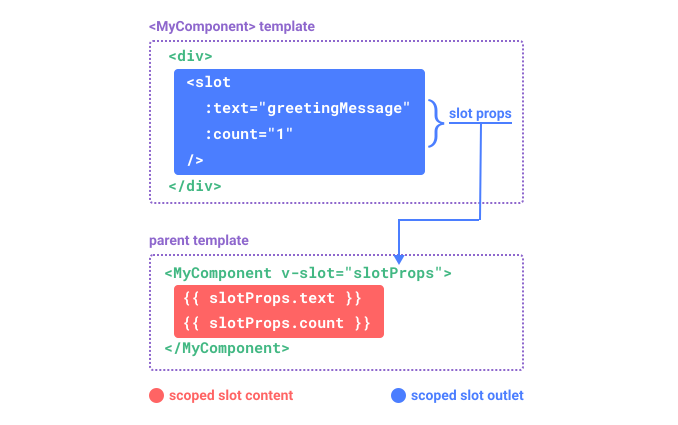
\includegraphics{./img/scoped-slots.1c6d5876.png} 
\end{center}
    


\columnratio{0.55}
\begin{paracol}{2}
 
\switchcolumn[0]*%%%%%%%
\href{https://play.vuejs.org/\#eNp9kMEKgzAMhl8l9OJlU3aVOhg7C3uAXsRlTtC2tFE2pO++dA5xMnZqk+b/8/2dxMnadBxQ5EL62rWWwCMN9qh021vjCMrn2fBNoya4OdNDkmarXhQnSstsVrOOC8LedhVhrEiuHca97wwVSsTj4oz1SvAUgKJpgqWZEj4IQoCvZm0Gtgghzss1BDvIbFkqdmID+CNdbbQnaBwitbop0fuqQSgguWPXmX+JePe1HT/QMtJBHnE51MZOCcjfzPx04JxsydPzp2Szxxo7vABY1I/p}{Try
it in the Playground}
\switchcolumn
\href{https://play.vuejs.org/\#eNp9kMEKgzAMhl8l9OJlU3aVOhg7C3uAXsRlTtC2tFE2pO++dA5xMnZqk+b/8/2dxMnadBxQ5EL62rWWwCMN9qh021vjCMrn2fBNoya4OdNDkmarXhQnSstsVrOOC8LedhVhrEiuHca97wwVSsTj4oz1SvAUgKJpgqWZEj4IQoCvZm0Gtgghzss1BDvIbFkqdmID+CNdbbQnaBwitbop0fuqQSgguWPXmX+JePe1HT/QMtJBHnE51MZOCcjfzPx04JxsydPzp2Szxxo7vABY1I/p}{在演练场中尝试一下}
\switchcolumn[0]*%%%%%%%
The props passed to the slot by the child are available as the value of
the corresponding \texttt{v-slot} directive, which can be accessed by
expressions inside the slot.
\switchcolumn
子组件传入插槽的 props 作为了 \texttt{v-slot}
指令的值,可以在插槽内的表达式中访问。
\switchcolumn[0]*%%%%%%%
You can think of a scoped slot as a function being passed into the child
component. The child component then calls it, passing props as
arguments:
\switchcolumn
你可以将作用域插槽类比为一个传入子组件的函数。子组件会将相应的 props
作为参数传给它:
\switchcolumn[0]*%%%%%%%
\begin{codeJs}
MyComponent({
  // 类比默认插槽,将其想成一个函数
  default: (slotProps) => {
    return `${slotProps.text} ${slotProps.count}`
  }
})
function MyComponent(slots) {
  const greetingMessage = 'hello'
  return `<div>${
    // 在插槽函数调用时传入 props
    slots.default({ text: greetingMessage, count: 1 })
  }</div>`
}
\end{codeJs}
\switchcolumn
\begin{codeJs}
MyComponent({
  // 类比默认插槽,将其想成一个函数
  default: (slotProps) => {
    return `${slotProps.text} ${slotProps.count}`
  }
})
function MyComponent(slots) {
  const greetingMessage = 'hello'
  return `<div>${
    // 在插槽函数调用时传入 props
    slots.default({ text: greetingMessage, count: 1 })
  }</div>`
}
\end{codeJs}
\switchcolumn[0]*%%%%%%%
In fact, this is very close to how scoped slots are compiled, and how
you would use scoped slots in manual
\href{https://vuejs.org/guide/extras/render-function.html}{render
functions}.
\switchcolumn
实际上,这已经和作用域插槽的最终代码编译结果、以及手动编写\href{https://cn.vuejs.org/guide/extras/render-function.html}{渲染函数}时使用作用域插槽的方式非常类似了。
\switchcolumn[0]*%%%%%%%
Notice how \texttt{v-slot="slotProps"} matches the slot function
signature. Just like with function arguments, we can use destructuring
in \texttt{v-slot}:
\switchcolumn
\texttt{v-slot="slotProps"}
可以类比这里的函数签名,和函数的参数类似,我们也可以在 \texttt{v-slot}
中使用解构:
\switchcolumn[0]*%%%%%%%
\begin{codeHtml}
<MyComponent v-slot="{ text, count }">
  {{ text }} {{ count }}
</MyComponent>
\end{codeHtml}
\switchcolumn
\begin{codeHtml}
<MyComponent v-slot="{ text, count }">
  {{ text }} {{ count }}
</MyComponent>
\end{codeHtml} 
\end{paracol}

\columnratio{0.55}
\begin{paracol}{2}
 
\switchcolumn[0]*%%%%%%%
\subsubsection{Named Scoped Slots}
\switchcolumn
\subsubsection{具名作用域插槽}
\switchcolumn[0]*%%%%%%%
Named scoped slots work similarly - slot props are accessible as the
value of the \texttt{v-slot} directive:
\texttt{v-slot:name="slotProps"}. When using the shorthand, it looks
like this:
\switchcolumn
具名作用域插槽的工作方式也是类似的,插槽 props 可以作为 \texttt{v-slot}
指令的值被访问到:\texttt{v-slot:name="slotProps"}。当使用缩写时是这样:
\switchcolumn[0]*%%%%%%%
\begin{codeHtml}
<MyComponent>
  <template #header="headerProps">
    {{ headerProps }}
  </template>
  <template #default="defaultProps">
    {{ defaultProps }}
  </template>
  <template #footer="footerProps">
    {{ footerProps }}
  </template>
</MyComponent>
\end{codeHtml}
\switchcolumn
\begin{codeHtml}
<MyComponent>
  <template #header="headerProps">
    {{ headerProps }}
  </template>
  <template #default="defaultProps">
    {{ defaultProps }}
  </template>
  <template #footer="footerProps">
    {{ footerProps }}
  </template>
</MyComponent>
\end{codeHtml}
\switchcolumn[0]*%%%%%%%
Passing props to a named slot:
\switchcolumn
向具名插槽中传入 props:
\switchcolumn[0]*%%%%%%%
\begin{codeHtml}
<slot name="header" message="hello"></slot>
\end{codeHtml}
\switchcolumn
\begin{codeHtml}
<slot name="header" message="hello"></slot>
\end{codeHtml}
\switchcolumn[0]*%%%%%%%
Note the \texttt{name} of a slot won't be included in the props because
it is reserved - so the resulting \texttt{headerProps} would be
\texttt{\{\ message:\ \textquotesingle{}hello\textquotesingle{}\ \}}.
\switchcolumn
注意插槽上的 \texttt{name} 是一个 Vue 特别保留的 attribute,不会作为
props 传递给插槽。因此最终 \texttt{headerProps} 的结果是
\texttt{\{\ message:\ \textquotesingle{}hello\textquotesingle{}\ \}}。
\switchcolumn[0]*%%%%%%%
If you are mixing named slots with the default scoped slot, you need to
use an explicit \texttt{\textless{}template\textgreater{}} tag for the
default slot. Attempting to place the \texttt{v-slot} directive directly
on the component will result in a compilation error. This is to avoid
any ambiguity about the scope of the props of the default slot. For
example:
\switchcolumn
如果你同时使用了具名插槽与默认插槽,则需要为默认插槽使用显式的
\texttt{\textless{}template\textgreater{}} 标签。尝试直接为组件添加
\texttt{v-slot} 指令将导致编译错误。这是为了避免因默认插槽的 props
的作用域而困惑。举例:
\switchcolumn[0]*%%%%%%%
\begin{codeHtml}
<!-- 该模板无法编译 -->
<template>
  <MyComponent v-slot="{ message }">
    <p>{{ message }}</p>
    <template #footer>
      <!-- message 属于默认插槽,此处不可用 -->
      <p>{{ message }}</p>
    </template>
  </MyComponent>
</template>
\end{codeHtml}
\switchcolumn
\begin{codeHtml}
<!-- 该模板无法编译 -->
<template>
  <MyComponent v-slot="{ message }">
    <p>{{ message }}</p>
    <template #footer>
      <!-- message 属于默认插槽,此处不可用 -->
      <p>{{ message }}</p>
    </template>
  </MyComponent>
</template>
\end{codeHtml}
\switchcolumn[0]*%%%%%%%
Using an explicit \texttt{\textless{}template\textgreater{}} tag for the
default slot helps to make it clear that the \texttt{message} prop is
not available inside the other slot:
\switchcolumn
为默认插槽使用显式的 \texttt{\textless{}template\textgreater{}}
标签有助于更清晰地指出 \texttt{message} 属性在其他插槽中不可用:
\switchcolumn[0]*%%%%%%%
\begin{codeHtml}
<template>
  <MyComponent>
    <!-- 使用显式的默认插槽 -->
    <template #default="{ message }">
      <p>{{ message }}</p>
    </template>
    <template #footer>
      <p>Here's some contact info</p>
    </template>
  </MyComponent>
</template>
\end{codeHtml}
\switchcolumn
\begin{codeHtml}
<template>
  <MyComponent>
    <!-- 使用显式的默认插槽 -->
    <template #default="{ message }">
      <p>{{ message }}</p>
    </template>
    <template #footer>
      <p>Here's some contact info</p>
    </template>
  </MyComponent>
</template>
\end{codeHtml}
\end{paracol}

\columnratio{0.55}
\begin{paracol}{2}
  
\switchcolumn[0]*%%%%%%%
\subsubsection{Fancy List Example}
\switchcolumn
\subsubsection{高级列表组件示例}
\switchcolumn[0]*%%%%%%%
You may be wondering what would be a good use case for scoped slots.
Here's an example: imagine a \texttt{\textless{}FancyList\textgreater{}}
component that renders a list of items - it may encapsulate the logic
for loading remote data, using the data to display a list, or even
advanced features like pagination or infinite scrolling. However, we
want it to be flexible with how each item looks and leave the styling of
each item to the parent component consuming it. So the desired usage may
look like this:
\switchcolumn
你可能想问什么样的场景才适合用到作用域插槽,这里我们来看一个
\texttt{\textless{}FancyList\textgreater{}}
组件的例子。它会渲染一个列表,并同时会封装一些加载远端数据的逻辑、使用数据进行列表渲染、或者是像分页或无限滚动这样更进阶的功能。然而我们希望它能够保留足够的灵活性,将对单个列表元素内容和样式的控制权留给使用它的父组件。我们期望的用法可能是这样的:
\switchcolumn[0]*%%%%%%%
\begin{codeHtml}
<FancyList :api-url="url" :per-page="10">
  <template #item="{ body, username, likes }">
    <div class="item">
      <p>{{ body }}</p>
      <p>by {{ username }} | {{ likes }} likes</p>
    </div>
  </template>
</FancyList>
\end{codeHtml}
\switchcolumn
\begin{codeHtml}
<FancyList :api-url="url" :per-page="10">
  <template #item="{ body, username, likes }">
    <div class="item">
      <p>{{ body }}</p>
      <p>by {{ username }} | {{ likes }} likes</p>
    </div>
  </template>
</FancyList>
\end{codeHtml}
\switchcolumn[0]*%%%%%%%
Inside \texttt{\textless{}FancyList\textgreater{}}, we can render the
same \texttt{\textless{}slot\textgreater{}} multiple times with
different item data (notice we are using \texttt{v-bind} to pass an
object as slot props):
\switchcolumn
在 \texttt{\textless{}FancyList\textgreater{}} 之中,我们可以多次渲染
\texttt{\textless{}slot\textgreater{}} 并每次都提供不同的数据
(注意我们这里使用了 \texttt{v-bind} 来传递插槽的 props):
\switchcolumn[0]*%%%%%%%
\begin{codeHtml}
<ul>
  <li v-for="item in items">
    <slot name="item" v-bind="item"></slot>
  </li>
</ul>
\end{codeHtml}
\switchcolumn
\begin{codeHtml}
<ul>
  <li v-for="item in items">
    <slot name="item" v-bind="item"></slot>
  </li>
</ul>
\end{codeHtml}
\switchcolumn[0]*%%%%%%%
\href{https://play.vuejs.org/\#eNqFU2Fv0zAQ/StHJtROapNuZTBCNwnQQKBpTGxCQss+uMml8+bYlu2UlZL/zjlp0lQa40sU3/nd3Xv3vA7eax0uSwziYGZTw7UDi67Up4nkhVbGwScm09U5tw5yowoYhFEX8cBBImdRgyQMHRwWWjCHdAKYbdFM83FpxEkS0DcJINZoxpotkCIHkySo7xOixcMep19KrmGustUISotGsgJHIPgDWqg6DKEyvoRUMGsJ4HG9HGX16bqpAlU1izy5baqDFegYweYroMttMwLAHx/Y9Kyan36RWUTN2+mjXfpbrei8k6SjdSuBYFOlMaNI6AeAtcflSrqx5b8xhkl4jMU7H0yVUCaGvVeH8+PjKYWqWnpf5DQYBTtb+fc612Awh2qzzGaBiUyVpBVpo7SFE8gw5xIv/Wl4M9gsbjCCQbuywe3+FuXl9iiqO7xpElEEhUofKFQo2mTGiFiOLr3jcpFImuiaF6hKNxzuw8lpw7kuEy6ZKJGK3TR6NluLYXBVqwRXQjkLn0ueIc3TLonyZ0sm4acqKVovKIbDCVQjGsb1qvyg2telU4Yzz6eHv6ARBWdwjVqUNCbbFjqgQn6aW1J8RKfJhDg+5/lStG4QHJZjnpO5XjT0BMqFu+uZ81yxjEQJw7A1kOA76FyZjaWBy0akvu8tCQKeQ+d7wsy5zLpz1FlzU3kW1QP+x40ApWgWAySEJTv6/NitNMkllcTakwCaZZ5ADEf6cROas/RhYVQps5igEpkZLwzRROmG04OjDBcj7+Js+vYQDo9e0uH1qzeY5/s1vtaaqG969+vTTrsmBTMLLv12nuy7l+d5W673SBzxkzlfhPdWSXokdZMkSFWhuUDzTTtOnk6CuG2fBEwI9etrHXOmRLJUE0/vMH14In5vH30sCS4Nkr+WmARdztHQ6Jr02dUFPtJ/lyxUVgq6/UzyO1olSj9jc+0DcaWxe/fqab/UT51Uu7Znjw6lbUn5QWtR6vtJQM//4zPUt+NOw+lGzCqo/gLm1QS8}{Try
it in the Playground}
\switchcolumn
\href{https://play.vuejs.org/\#eNqFU2Fv0zAQ/StHJtROapNuZTBCNwnQQKBpTGxCQss+uMml8+bYlu2UlZL/zjlp0lQa40sU3/nd3Xv3vA7eax0uSwziYGZTw7UDi67Up4nkhVbGwScm09U5tw5yowoYhFEX8cBBImdRgyQMHRwWWjCHdAKYbdFM83FpxEkS0DcJINZoxpotkCIHkySo7xOixcMep19KrmGustUISotGsgJHIPgDWqg6DKEyvoRUMGsJ4HG9HGX16bqpAlU1izy5baqDFegYweYroMttMwLAHx/Y9Kyan36RWUTN2+mjXfpbrei8k6SjdSuBYFOlMaNI6AeAtcflSrqx5b8xhkl4jMU7H0yVUCaGvVeH8+PjKYWqWnpf5DQYBTtb+fc612Awh2qzzGaBiUyVpBVpo7SFE8gw5xIv/Wl4M9gsbjCCQbuywe3+FuXl9iiqO7xpElEEhUofKFQo2mTGiFiOLr3jcpFImuiaF6hKNxzuw8lpw7kuEy6ZKJGK3TR6NluLYXBVqwRXQjkLn0ueIc3TLonyZ0sm4acqKVovKIbDCVQjGsb1qvyg2telU4Yzz6eHv6ARBWdwjVqUNCbbFjqgQn6aW1J8RKfJhDg+5/lStG4QHJZjnpO5XjT0BMqFu+uZ81yxjEQJw7A1kOA76FyZjaWBy0akvu8tCQKeQ+d7wsy5zLpz1FlzU3kW1QP+x40ApWgWAySEJTv6/NitNMkllcTakwCaZZ5ADEf6cROas/RhYVQps5igEpkZLwzRROmG04OjDBcj7+Js+vYQDo9e0uH1qzeY5/s1vtaaqG969+vTTrsmBTMLLv12nuy7l+d5W673SBzxkzlfhPdWSXokdZMkSFWhuUDzTTtOnk6CuG2fBEwI9etrHXOmRLJUE0/vMH14In5vH30sCS4Nkr+WmARdztHQ6Jr02dUFPtJ/lyxUVgq6/UzyO1olSj9jc+0DcaWxe/fqab/UT51Uu7Znjw6lbUn5QWtR6vtJQM//4zPUt+NOw+lGzCqo/gLm1QS8}{在演练场中尝试一下}
\end{paracol}


\columnratio{0.55}
\begin{paracol}{2}
 
\switchcolumn[0]*%%%%%%%
\subsubsection{Renderless Components}
\switchcolumn
\subsubsection{无渲染组件}
\switchcolumn[0]*%%%%%%%
The \texttt{\textless{}FancyList\textgreater{}} use case we discussed
above encapsulates both reusable logic (data fetching, pagination etc.)
and visual output, while delegating part of the visual output to the
consumer component via scoped slots.
\switchcolumn
上面的 \texttt{\textless{}FancyList\textgreater{}}
案例同时封装了可重用的逻辑 (数据获取、分页等)
和视图输出,但也将部分视图输出通过作用域插槽交给了消费者组件来管理。
\switchcolumn[0]*%%%%%%%
If we push this concept a bit further, we can come up with components
that only encapsulate logic and do not render anything by themselves -
visual output is fully delegated to the consumer component with scoped
slots. We call this type of component a \textbf{Renderless Component}.
\switchcolumn
如果我们将这个概念拓展一下,可以想象的是,一些组件可能只包括了逻辑而不需要自己渲染内容,视图输出通过作用域插槽全权交给了消费者组件。我们将这种类型的组件称为\textbf{无渲染组件}。
\switchcolumn[0]*%%%%%%%
An example renderless component could be one that encapsulates the logic
of tracking the current mouse position:
\switchcolumn
这里有一个无渲染组件的例子,一个封装了追踪当前鼠标位置逻辑的组件:
\switchcolumn[0]*%%%%%%%
\begin{codeHtml}
<MouseTracker v-slot="{ x, y }">
  Mouse is at: {{ x }}, {{ y }}
</MouseTracker>
\end{codeHtml}
\switchcolumn
\begin{codeHtml}
<MouseTracker v-slot="{ x, y }">
  Mouse is at: {{ x }}, {{ y }}
</MouseTracker>
\end{codeHtml}
\switchcolumn[0]*%%%%%%%
\href{https://play.vuejs.org/\#eNqNUcFqhDAQ/ZUhF12w2rO4Cz301t5aaCEX0dki1SQko6uI/96J7i4qLPQQmHmZ9+Y9ZhQvxsRdiyIVmStsZQgcUmtOUlWN0ZbgXbcOP2xe/KKFs9UNBHGyBj09kCpLFj4zuSFsTJ0T+o6yjUb35GpNRylG6CMYYJKCpwAkzWNQOcgphZG/YZoiX/DQNAttFjMrS+6LRCT2rh6HGsHiOQKtmKIIS19+qmZpYLrmXIKxM1Vo5Yj9HD0vfD7ckGGF3LDWlOyHP/idYPQCfdzldTtjscl/8MuDww78lsqHVHdTYXjwCpdKlfoS52X52qGit8oRKrRhwHYdNrrDILouPbCNVZCtgJ1n/6Xx8JYAmT8epD3fr5cC0oGLQYpkd4zpD27R0vA=}{Try
it in the Playground}
\switchcolumn
\href{https://play.vuejs.org/\#eNqNUcFqhDAQ/ZUhF12w2rO4Cz301t5aaCEX0dki1SQko6uI/96J7i4qLPQQmHmZ9+Y9ZhQvxsRdiyIVmStsZQgcUmtOUlWN0ZbgXbcOP2xe/KKFs9UNBHGyBj09kCpLFj4zuSFsTJ0T+o6yjUb35GpNRylG6CMYYJKCpwAkzWNQOcgphZG/YZoiX/DQNAttFjMrS+6LRCT2rh6HGsHiOQKtmKIIS19+qmZpYLrmXIKxM1Vo5Yj9HD0vfD7ckGGF3LDWlOyHP/idYPQCfdzldTtjscl/8MuDww78lsqHVHdTYXjwCpdKlfoS52X52qGit8oRKrRhwHYdNrrDILouPbCNVZCtgJ1n/6Xx8JYAmT8epD3fr5cC0oGLQYpkd4zpD27R0vA=}{在演练场中尝试一下}
\switchcolumn[0]*%%%%%%%
While an interesting pattern, most of what can be achieved with
Renderless Components can be achieved in a more efficient fashion with
Composition API, without incurring the overhead of extra component
nesting. Later, we will see how we can implement the same mouse tracking
functionality as a
\href{https://vuejs.org/guide/reusability/composables.html}{Composable}.
\switchcolumn
虽然这个模式很有趣,但大部分能用无渲染组件实现的功能都可以通过组合式 API
以另一种更高效的方式实现,并且还不会带来额外组件嵌套的开销。之后我们会在\href{https://cn.vuejs.org/guide/reusability/composables.html}{组合式函数}一章中介绍如何更高效地实现追踪鼠标位置的功能。
\switchcolumn[0]*%%%%%%%
That said, scoped slots are still useful in cases where we need to both
encapsulate logic \textbf{and} compose visual output, like in the
\texttt{\textless{}FancyList\textgreater{}} example.
\switchcolumn
尽管如此,作用域插槽在需要\textbf{同时}封装逻辑、组合视图界面时还是很有用,就像上面的
\texttt{\textless{}FancyList\textgreater{}} 组件那样。
\end{paracol}



\columnratio{0.55}
\begin{paracol}{2}
 
\end{paracol}

% \columnratio{0.55}
\begin{paracol}{2}
\switchcolumn[0]*%%%%%%%
\section{Provide / Inject}
\switchcolumn
\section{依赖注入}
\switchcolumn[0]*%%%%%%%
\begin{quote}
This page assumes you've already read the
\href{https://vuejs.org/guide/essentials/component-basics.html}{Components
Basics}. Read that first if you are new to components.
\end{quote}
\switchcolumn
\begin{quote}
此章节假设你已经看过了\href{https://cn.vuejs.org/guide/essentials/component-basics.html}{组件基础}。若你还不了解组件是什么,请先阅读该章节。
\end{quote}
\switchcolumn[0]*%%%%%%%
\subsection{Prop Drilling}
\switchcolumn
\subsection{Prop 逐级透传问题}
\switchcolumn[0]*%%%%%%%
Usually, when we need to pass data from the parent to a child component,
we use \href{https://vuejs.org/guide/components/props.html}{props}.
However, imagine the case where we have a large component tree, and a
deeply nested component needs something from a distant ancestor
component. With only props, we would have to pass the same prop across
the entire parent chain:
\switchcolumn
通常情况下,当我们需要从父组件向子组件传递数据时,会使用
\href{https://cn.vuejs.org/guide/components/props.html}{props}。想象一下这样的结构:有一些多层级嵌套的组件,形成了一颗巨大的组件树,而某个深层的子组件需要一个较远的祖先组件中的部分数据。在这种情况下,如果仅使用
props 则必须将其沿着组件链逐级传递下去,这会非常麻烦:
\end{paracol}

\begin{center} 
\includegraphics{./img/prop-drilling.11201220.png} 
\end{center}

\columnratio{0.55}
\begin{paracol}{2}
\switchcolumn[0]*%%%%%%%
Notice although the \texttt{\textless{}Footer\textgreater{}} component
may not care about these props at all, it still needs to declare and
pass them along just so \texttt{\textless{}DeepChild\textgreater{}} can
access them. If there is a longer parent chain, more components would be
affected along the way. This is called "props drilling" and definitely
isn't fun to deal with.
\switchcolumn
注意,虽然这里的 \texttt{\textless{}Footer\textgreater{}}
组件可能根本不关心这些 props,但为了使
\texttt{\textless{}DeepChild\textgreater{}}
能访问到它们,仍然需要定义并向下传递。如果组件链路非常长,可能会影响到更多这条路上的组件。这一问题被称为``prop
逐级透传'',显然是我们希望尽量避免的情况。
\switchcolumn[0]*%%%%%%%
We can solve props drilling with \texttt{provide} and \texttt{inject}. A
parent component can serve as a \textbf{dependency provider} for all its
descendants. Any component in the descendant tree, regardless of how
deep it is, can \textbf{inject} dependencies provided by components up
in its parent chain.
\switchcolumn
\texttt{provide} 和 \texttt{inject} 可以帮助我们解决这一问题。
\href{https://cn.vuejs.org/guide/components/provide-inject.html\#footnote-1}{{[}1{]}}
一个父组件相对于其所有的后代组件,会作为\textbf{依赖提供者}。任何后代的组件树,无论层级有多深,都可以\textbf{注入}由父组件提供给整条链路的依赖。
\end{paracol}

\begin{center} 
\includegraphics{./img/provide-inject.3e0505e4.png} 
\end{center}

\columnratio{0.55}
\begin{paracol}{2}
 
\switchcolumn[0]*%%%%%%%
\subsection{Provide}
\switchcolumn
\subsection{Provide (提供)}
\switchcolumn[0]*%%%%%%%
To provide data to a component's descendants, use the
\href{https://vuejs.org/api/composition-api-dependency-injection.html\#provide}{\texttt{provide()}}
function:
\switchcolumn
要为组件后代提供数据,需要使用到
\href{https://cn.vuejs.org/api/composition-api-dependency-injection.html\#provide}{\texttt{provide()}}
函数:
\switchcolumn[0]*%%%%%%%
\begin{codeHtml}
<script setup>
import { provide } from 'vue'
provide(/* 注入名 */ 'message', /* 值 */ 'hello!')
</script>
\end{codeHtml}
\switchcolumn
\begin{codeHtml}
<script setup>
import { provide } from 'vue'
provide(/* 注入名 */ 'message', /* 值 */ 'hello!')
</script>
\end{codeHtml}
\switchcolumn[0]*%%%%%%%
If not using \texttt{\textless{}script\ setup\textgreater{}}, make sure
\texttt{provide()} is called synchronously inside \texttt{setup()}:
\switchcolumn
如果不使用 \texttt{\textless{}script\ setup\textgreater{}},请确保
\texttt{provide()} 是在 \texttt{setup()} 同步调用的:
\switchcolumn[0]*%%%%%%%
\begin{codeJs}
import { provide } from 'vue'
export default {
  setup() {
    provide(/* 注入名 */ 'message', /* 值 */ 'hello!')
  }
}
\end{codeJs}
\switchcolumn
\begin{codeJs}
import { provide } from 'vue'
export default {
  setup() {
    provide(/* 注入名 */ 'message', /* 值 */ 'hello!')
  }
}
\end{codeJs}
\switchcolumn[0]*%%%%%%%
The \texttt{provide()} function accepts two arguments. The first
argument is called the \textbf{injection key}, which can be a string or
a \texttt{Symbol}. The injection key is used by descendant components to
lookup the desired value to inject. A single component can call
\texttt{provide()} multiple times with different injection keys to
provide different values.
\switchcolumn
\texttt{provide()}
函数接收两个参数。第一个参数被称为\textbf{注入名},可以是一个字符串或是一个
\texttt{Symbol}。后代组件会用注入名来查找期望注入的值。一个组件可以多次调用
\texttt{provide()},使用不同的注入名,注入不同的依赖值。
\switchcolumn[0]*%%%%%%%
The second argument is the provided value. The value can be of any type,
including reactive state such as refs:
\switchcolumn
第二个参数是提供的值,值可以是任意类型,包括响应式的状态,比如一个 ref:
\switchcolumn[0]*%%%%%%%
\begin{codeJs}
import { ref, provide } from 'vue'
const count = ref(0)
provide('key', count)
\end{codeJs}
\switchcolumn
\begin{codeJs}
import { ref, provide } from 'vue'
const count = ref(0)
provide('key', count)
\end{codeJs}
\switchcolumn[0]*%%%%%%%
Providing reactive values allows the descendant components using the
provided value to establish a reactive connection to the provider
component.
\switchcolumn
提供的响应式状态使后代组件可以由此和提供者建立响应式的联系。
\end{paracol}

\columnratio{0.55}
\begin{paracol}{2} 
\switchcolumn[0]*%%%%%%%
\subsection{App-level Provide}
\switchcolumn
\subsection{应用层 Provide}
\switchcolumn[0]*%%%%%%%
In addition to providing data in a component, we can also provide at the
app level:
\switchcolumn
除了在一个组件中提供依赖,我们还可以在整个应用层面提供依赖:
\switchcolumn[0]*%%%%%%%
\begin{codeJs}
import { createApp } from 'vue'
const app = createApp({})
app.provide(/* 注入名 */ 'message', /* 值 */ 'hello!')
\end{codeJs}
\switchcolumn
\begin{codeJs}
import { createApp } from 'vue'
const app = createApp({})
app.provide(/* 注入名 */ 'message', /* 值 */ 'hello!')
\end{codeJs}
\switchcolumn[0]*%%%%%%%
App-level provides are available to all components rendered in the app.
This is especially useful when writing
\href{https://vuejs.org/guide/reusability/plugins.html}{plugins}, as
plugins typically wouldn't be able to provide values using components.
\switchcolumn
在应用级别提供的数据在该应用内的所有组件中都可以注入。这在你编写\href{https://cn.vuejs.org/guide/reusability/plugins.html}{插件}时会特别有用,因为插件一般都不会使用组件形式来提供值。
\end{paracol}

\columnratio{0.55}
\begin{paracol}{2}
 
\switchcolumn[0]*%%%%%%%
\subsection{Inject}
\switchcolumn
\subsection{Inject (注入)}
\switchcolumn[0]*%%%%%%%
To inject data provided by an ancestor component, use the
\href{https://vuejs.org/api/composition-api-dependency-injection.html\#inject}{\texttt{inject()}}
function:
\switchcolumn
要注入上层组件提供的数据,需使用
\href{https://cn.vuejs.org/api/composition-api-dependency-injection.html\#inject}{\texttt{inject()}}
函数:
\switchcolumn[0]*%%%%%%%
\begin{codeHtml}
<script setup>
import { inject } from 'vue'
const message = inject('message')
</script>
\end{codeHtml}
\switchcolumn
\begin{codeHtml}
<script setup>
import { inject } from 'vue'
const message = inject('message')
</script>
\end{codeHtml}
\switchcolumn[0]*%%%%%%%
If the provided value is a ref, it will be injected as-is and will
\textbf{not} be automatically unwrapped. This allows the injector
component to retain the reactivity connection to the provider component.
\switchcolumn
如果提供的值是一个 ref,注入进来的会是该 ref
对象,而\textbf{不会}自动解包为其内部的值。这使得注入方组件能够通过 ref
对象保持了和供给方的响应性链接。
\switchcolumn[0]*%%%%%%%
\href{https://play.vuejs.org/\#eNqFUUFugzAQ/MrKF1IpxfeIVKp66Kk/8MWFDXYFtmUbpArx967BhURRU9/WOzO7MzuxV+fKcUB2YlWovXYRAsbBvQije2d9hAk8Xo7gvB11gzDDxdseCuIUG+ZN6a7JjZIvVRIlgDCcw+d3pmvTglz1okJ499I0C3qB1dJQT9YRooVaSdNiACWdQ5OICj2WwtTWhAg9hiBbhHNSOxQKu84WT8LkNQ9FBhTHXyg1K75aJHNUROxdJyNSBVBp44YI43NvG+zOgmWWYGt7dcipqPhGZEe2ef07wN3lltD+lWN6tNkV/37+rdKjK2rzhRTt7f3u41xhe37/xJZGAL2PLECXa9NKdD/a6QTTtGnP88LgiXJtYv4BaLHhvg==}{Full
provide + inject Example with Reactivity}
\switchcolumn
\href{https://play.vuejs.org/\#eNqFUUFugzAQ/MrKF1IpxfeIVKp66Kk/8MWFDXYFtmUbpArx967BhURRU9/WOzO7MzuxV+fKcUB2YlWovXYRAsbBvQije2d9hAk8Xo7gvB11gzDDxdseCuIUG+ZN6a7JjZIvVRIlgDCcw+d3pmvTglz1okJ499I0C3qB1dJQT9YRooVaSdNiACWdQ5OICj2WwtTWhAg9hiBbhHNSOxQKu84WT8LkNQ9FBhTHXyg1K75aJHNUROxdJyNSBVBp44YI43NvG+zOgmWWYGt7dcipqPhGZEe2ef07wN3lltD+lWN6tNkV/37+rdKjK2rzhRTt7f3u41xhe37/xJZGAL2PLECXa9NKdD/a6QTTtGnP88LgiXJtYv4BaLHhvg==}{带有响应性的
provide + inject 完整示例}
\switchcolumn[0]*%%%%%%%
Again, if not using \texttt{\textless{}script\ setup\textgreater{}},
\texttt{inject()} should only be called synchronously inside
\texttt{setup()}:
\switchcolumn
同样的,如果没有使用
\texttt{\textless{}script\ setup\textgreater{}},\texttt{inject()}
需要在 \texttt{setup()} 内同步调用:
\switchcolumn[0]*%%%%%%%
\begin{codeJs}
import { inject } from 'vue'
export default {
  setup() {
    const message = inject('message')
    return { message }
  }
}
\end{codeJs}
\switchcolumn
\begin{codeJs}
import { inject } from 'vue'
export default {
  setup() {
    const message = inject('message')
    return { message }
  }
}
\end{codeJs}
\end{paracol}

\columnratio{0.55}
\begin{paracol}{2}
\switchcolumn[0]*%%%%%%%
\subsubsection{Injection Default Values}
\switchcolumn
\subsubsection{注入默认值}
\switchcolumn[0]*%%%%%%%
By default, \texttt{inject} assumes that the injected key is provided
somewhere in the parent chain. In the case where the key is not
provided, there will be a runtime warning.
\switchcolumn
默认情况下,\texttt{inject}
假设传入的注入名会被某个祖先链上的组件提供。如果该注入名的确没有任何组件提供,则会抛出一个运行时警告。
\switchcolumn[0]*%%%%%%%
If we want to make an injected property work with optional providers, we
need to declare a default value, similar to props:
\switchcolumn
如果在注入一个值时不要求必须有提供者,那么我们应该声明一个默认值,和
props 类似:
\switchcolumn[0]*%%%%%%%
\begin{codeJs}
// 如果没有祖先组件提供 "message"
// `value` 会是 "这是默认值"
const value = inject('message', '这是默认值')
\end{codeJs}
\switchcolumn
\begin{codeJs}
// 如果没有祖先组件提供 "message"
// `value` 会是 "这是默认值"
const value = inject('message', '这是默认值')
\end{codeJs}
\switchcolumn[0]*%%%%%%%
In some cases, the default value may need to be created by calling a
function or instantiating a new class. To avoid unnecessary computation
or side effects in case the optional value is not used, we can use a
factory function for creating the default value:
\switchcolumn
在一些场景中,默认值可能需要通过调用一个函数或初始化一个类来取得。为了避免在用不到默认值的情况下进行不必要的计算或产生副作用,我们可以使用工厂函数来创建默认值:
\switchcolumn[0]*%%%%%%%
\begin{codeJs}
const value = inject('key', () => new ExpensiveClass(), true)
\end{codeJs}
\switchcolumn
\begin{codeJs}
const value = inject('key', () => new ExpensiveClass(), true)
\end{codeJs}
\switchcolumn[0]*%%%%%%%
The third parameter indicates the default value should be treated as a
factory function.
\switchcolumn
第三个参数表示默认值应该被当作一个工厂函数。
\end{paracol}

\columnratio{0.55}
\begin{paracol}{2}
 
\switchcolumn[0]*%%%%%%%
\subsection{Working with Reactivity}
\switchcolumn
\subsection{和响应式数据配合使用}
\switchcolumn[0]*%%%%%%%
When using reactive provide / inject values, \textbf{it is recommended
to keep any mutations to reactive state inside of the *provider*
whenever possible}. This ensures that the provided state and its
possible mutations are co-located in the same component, making it
easier to maintain in the future.
\switchcolumn
当提供 /
注入响应式的数据时,\textbf{建议尽可能将任何对响应式状态的变更都保持在供给方组件中}。这样可以确保所提供状态的声明和变更操作都内聚在同一个组件内,使其更容易维护。
\switchcolumn[0]*%%%%%%%
There may be times when we need to update the data from an injector
component. In such cases, we recommend providing a function that is
responsible for mutating the state:
\switchcolumn
有的时候,我们可能需要在注入方组件中更改数据。在这种情况下,我们推荐在供给方组件内声明并提供一个更改数据的方法函数:
\switchcolumn[0]*%%%%%%%
\begin{codeHtml}
<!-- 在供给方组件内 -->
<script setup>
import { provide, ref } from 'vue'
const location = ref('North Pole')
function updateLocation() {
  location.value = 'South Pole'
}
provide('location', {
  location,
  updateLocation
})
</script>
\end{codeHtml}
\switchcolumn
\begin{codeHtml}
<!-- 在供给方组件内 -->
<script setup>
import { provide, ref } from 'vue'
const location = ref('North Pole')
function updateLocation() {
  location.value = 'South Pole'
}
provide('location', {
  location,
  updateLocation
})
</script>
\end{codeHtml}
\switchcolumn[0]*%%%%%%%
\begin{codeHtml}
<!-- 在注入方组件 -->
<script setup>
import { inject } from 'vue'
const { location, updateLocation } = inject('location')
</script>
<template>
  <button @click="updateLocation">{{ location }}</button>
</template>
\end{codeHtml}
\switchcolumn
\begin{codeHtml}
<!-- 在注入方组件 -->
<script setup>
import { inject } from 'vue'
const { location, updateLocation } = inject('location')
</script>
<template>
  <button @click="updateLocation">{{ location }}</button>
</template>
\end{codeHtml}
\switchcolumn[0]*%%%%%%%
Finally, you can wrap the provided value with
\href{https://vuejs.org/api/reactivity-core.html\#readonly}{\texttt{readonly()}}
if you want to ensure that the data passed through \texttt{provide}
cannot be mutated by the injector component.
\switchcolumn
最后,如果你想确保提供的数据不能被注入方的组件更改,你可以使用
\href{https://cn.vuejs.org/api/reactivity-core.html\#readonly}{\texttt{readonly()}}
来包装提供的值。
\switchcolumn[0]*%%%%%%%
\begin{codeHtml}
<script setup>
import { ref, provide, readonly } from 'vue'
const count = ref(0)
provide('read-only-count', readonly(count))
</script>
\end{codeHtml}
\switchcolumn
\begin{codeHtml}
<script setup>
import { ref, provide, readonly } from 'vue'
const count = ref(0)
provide('read-only-count', readonly(count))
</script>
\end{codeHtml}
\end{paracol}

\columnratio{0.55}
\begin{paracol}{2}
 
\switchcolumn[0]*%%%%%%%
\subsection{Working with Symbol Keys}
\switchcolumn
\subsection{使用 Symbol 作注入名}
\switchcolumn[0]*%%%%%%%
So far, we have been using string injection keys in the examples. If you
are working in a large application with many dependency providers, or
you are authoring components that are going to be used by other
developers, it is best to use Symbol injection keys to avoid potential
collisions.
\switchcolumn
至此,我们已经了解了如何使用字符串作为注入名。但如果你正在构建大型的应用,包含非常多的依赖提供,或者你正在编写提供给其他开发者使用的组件库,建议最好使用
Symbol 来作为注入名以避免潜在的冲突。
\switchcolumn[0]*%%%%%%%
It's recommended to export the Symbols in a dedicated file:
\switchcolumn
我们通常推荐在一个单独的文件中导出这些注入名 Symbol:
\switchcolumn[0]*%%%%%%%
\begin{codeJs}
// keys.js
export const myInjectionKey = Symbol()
\end{codeJs}
\switchcolumn
\begin{codeJs}
// keys.js
export const myInjectionKey = Symbol()
\end{codeJs}
\switchcolumn[0]*%%%%%%%
\begin{codeHtml}
// 在供给方组件中
import { provide } from 'vue'
import { myInjectionKey } from './keys.js'
provide(myInjectionKey, { /*
  要提供的数据
*/ });
\end{codeHtml}
\switchcolumn
\begin{codeHtml}
// 在供给方组件中
import { provide } from 'vue'
import { myInjectionKey } from './keys.js'
provide(myInjectionKey, { /*
  要提供的数据
*/ });
\end{codeHtml}
\switchcolumn[0]*%%%%%%%
\begin{codeJs}
// 注入方组件
import { inject } from 'vue'
import { myInjectionKey } from './keys.js'
const injected = inject(myInjectionKey)
\end{codeJs}
\switchcolumn
\begin{codeJs}
// 注入方组件
import { inject } from 'vue'
import { myInjectionKey } from './keys.js'
const injected = inject(myInjectionKey)
\end{codeJs}
\switchcolumn[0]*%%%%%%%
See also:
\href{https://vuejs.org/guide/typescript/composition-api.html\#typing-provide-inject}{Typing
Provide / Inject}
\switchcolumn
TypeScript
用户请参考:\href{https://cn.vuejs.org/guide/typescript/composition-api.html\#typing-provide-inject}{为
Provide / Inject 标注类型}
\switchcolumn[0]*%%%%%%%
\href{https://github.com/vuejs/docs/edit/main/src/guide/components/provide-inject.md}{Edit
this page on GitHub}
\switchcolumn
\textbf{译者注}{[}1{]} 在本章及后续章节中,``\textbf{提供}''将成为对应
Provide 的一个专有概念
\end{paracol}
% \columnratio{0.55}
\begin{paracol}{2}
 
\switchcolumn[0]*%%%%%%%
\section{Async Components}
\switchcolumn
\section{异步组件}
\switchcolumn[0]*%%%%%%%
\subsection{Basic Usage}
\switchcolumn
\subsection{基本用法}
\switchcolumn[0]*%%%%%%%
In large applications, we may need to divide the app into smaller chunks
and only load a component from the server when it's needed. To make that
possible, Vue has a
\href{https://vuejs.org/api/general.html\#defineasynccomponent}{\texttt{defineAsyncComponent}}
function:
\switchcolumn
在大型项目中,我们可能需要拆分应用为更小的块,并仅在需要时再从服务器加载相关组件。Vue
提供了
\href{https://cn.vuejs.org/api/general.html\#defineasynccomponent}{\texttt{defineAsyncComponent}}
方法来实现此功能:
\switchcolumn[0]*%%%%%%%
\begin{codeJs}
import { defineAsyncComponent } from 'vue'
const AsyncComp = defineAsyncComponent(() => {
  return new Promise((resolve, reject) => {
    // ...从服务器获取组件
    resolve(/* 获取到的组件 */)
  })
})
// ... 像使用其他一般组件一样使用 `AsyncComp`
\end{codeJs}
\switchcolumn
\begin{codeJs}
import { defineAsyncComponent } from 'vue'
const AsyncComp = defineAsyncComponent(() => {
  return new Promise((resolve, reject) => {
    // ...从服务器获取组件
    resolve(/* 获取到的组件 */)
  })
})
// ... 像使用其他一般组件一样使用 `AsyncComp`
\end{codeJs}
\switchcolumn[0]*%%%%%%%
As you can see, \texttt{defineAsyncComponent} accepts a loader function
that returns a Promise. The Promise's \texttt{resolve} callback should
be called when you have retrieved your component definition from the
server. You can also call \texttt{reject(reason)} to indicate the load
has failed.
\switchcolumn
如你所见,\texttt{defineAsyncComponent} 方法接收一个返回 Promise
的加载函数。这个 Promise 的 \texttt{resolve}
回调方法应该在从服务器获得组件定义时调用。你也可以调用
\texttt{reject(reason)} 表明加载失败。
\switchcolumn[0]*%%%%%%%
\href{https://developer.mozilla.org/en-US/docs/Web/JavaScript/Reference/Operators/import}{ES
module dynamic import} also returns a Promise, so most of the time we
will use it in combination with \texttt{defineAsyncComponent}. Bundlers
like Vite and webpack also support the syntax (and will use it as bundle
split points), so we can use it to import Vue SFCs:
\switchcolumn
\href{https://developer.mozilla.org/en-US/docs/Web/JavaScript/Reference/Operators/import}{ES
模块动态导入}也会返回一个 Promise,所以多数情况下我们会将它和
\texttt{defineAsyncComponent} 搭配使用。类似 Vite 和 Webpack
这样的构建工具也支持此语法
(并且会将它们作为打包时的代码分割点),因此我们也可以用它来导入 Vue
单文件组件:
\switchcolumn[0]*%%%%%%%
\begin{codeJs}
import { defineAsyncComponent } from 'vue'
const AsyncComp = defineAsyncComponent(() =>
  import('./components/MyComponent.vue')
)
\end{codeJs}
\switchcolumn
\begin{codeJs}
import { defineAsyncComponent } from 'vue'
const AsyncComp = defineAsyncComponent(() =>
  import('./components/MyComponent.vue')
)
\end{codeJs}
\switchcolumn[0]*%%%%%%%
The resulting \texttt{AsyncComp} is a wrapper component that only calls
the loader function when it is actually rendered on the page. In
addition, it will pass along any props and slots to the inner component,
so you can use the async wrapper to seamlessly replace the original
component while achieving lazy loading.
\switchcolumn
最后得到的 \texttt{AsyncComp}
是一个外层包装过的组件,仅在页面需要它渲染时才会调用加载内部实际组件的函数。它会将接收到的
props
和插槽传给内部组件,所以你可以使用这个异步的包装组件无缝地替换原始组件,同时实现延迟加载。
\switchcolumn[0]*%%%%%%%
As with normal components, async components can be
\href{https://vuejs.org/guide/components/registration.html\#global-registration}{registered
globally} using \texttt{app.component()}:
\switchcolumn
与普通组件一样,异步组件可以使用 \texttt{app.component()}
\href{https://cn.vuejs.org/guide/components/registration.html\#global-registration}{全局注册}:
\switchcolumn[0]*%%%%%%%
\begin{codeJs}
app.component('MyComponent', defineAsyncComponent(() =>
  import('./components/MyComponent.vue')
))
\end{codeJs}
\switchcolumn
\begin{codeJs}
app.component('MyComponent', defineAsyncComponent(() =>
  import('./components/MyComponent.vue')
))
\end{codeJs}
\switchcolumn[0]*%%%%%%%
They can also be defined directly inside their parent component:
\switchcolumn
也可以直接在父组件中直接定义它们:
\switchcolumn[0]*%%%%%%%
\begin{codeHtml}
<script setup>
import { defineAsyncComponent } from 'vue'
const AdminPage = defineAsyncComponent(() =>
  import('./components/AdminPageComponent.vue')
)
</script>
<template>
  <AdminPage />
</template>
\end{codeHtml}
\switchcolumn
\begin{codeHtml}
<script setup>
import { defineAsyncComponent } from 'vue'
const AdminPage = defineAsyncComponent(() =>
  import('./components/AdminPageComponent.vue')
)
</script>
<template>
  <AdminPage />
</template>
\end{codeHtml}
\end{paracol}

\columnratio{0.55}
\begin{paracol}{2}
 
\switchcolumn[0]*%%%%%%%
\subsection{Loading and Error States}
\switchcolumn
\subsection{加载与错误状态}
\switchcolumn[0]*%%%%%%%
Asynchronous operations inevitably involve loading and error states -
\texttt{defineAsyncComponent()} supports handling these states via
advanced options:
\switchcolumn
异步操作不可避免地会涉及到加载和错误状态,因此
\texttt{defineAsyncComponent()} 也支持在高级选项中处理这些状态:
\switchcolumn[0]*%%%%%%%
\begin{codeJs}
const AsyncComp = defineAsyncComponent({
  // 加载函数
  loader: () => import('./Foo.vue'),
  // 加载异步组件时使用的组件
  loadingComponent: LoadingComponent,
  // 展示加载组件前的延迟时间,默认为 200ms
  delay: 200,
  // 加载失败后展示的组件
  errorComponent: ErrorComponent,
  // 如果提供了一个 timeout 时间限制,并超时了
  // 也会显示这里配置的报错组件,默认值是:Infinity
  timeout: 3000
})
\end{codeJs}
\switchcolumn
\begin{codeJs}
const AsyncComp = defineAsyncComponent({
  // 加载函数
  loader: () => import('./Foo.vue'),
  // 加载异步组件时使用的组件
  loadingComponent: LoadingComponent,
  // 展示加载组件前的延迟时间,默认为 200ms
  delay: 200,
  // 加载失败后展示的组件
  errorComponent: ErrorComponent,
  // 如果提供了一个 timeout 时间限制,并超时了
  // 也会显示这里配置的报错组件,默认值是:Infinity
  timeout: 3000
})
\end{codeJs}
\switchcolumn[0]*%%%%%%%
If a loading component is provided, it will be displayed first while the
inner component is being loaded. There is a default 200ms delay before
the loading component is shown - this is because on fast networks, an
instant loading state may get replaced too fast and end up looking like
a flicker.
\switchcolumn
如果提供了一个加载组件,它将在内部组件加载时先行显示。在加载组件显示之前有一个默认的
200ms
延迟------这是因为在网络状况较好时,加载完成得很快,加载组件和最终组件之间的替换太快可能产生闪烁,反而影响用户感受。
\switchcolumn[0]*%%%%%%%
If an error component is provided, it will be displayed when the Promise
returned by the loader function is rejected. You can also specify a
timeout to show the error component when the request is taking too long.
\switchcolumn
如果提供了一个报错组件,则它会在加载器函数返回的 Promise
抛错时被渲染。你还可以指定一个超时时间,在请求耗时超过指定时间时也会渲染报错组件。
\end{paracol}

\columnratio{0.55}
\begin{paracol}{2}
 
\switchcolumn[0]*%%%%%%%
\subsection{Using with Suspense}
\switchcolumn
\subsection{搭配 Suspense 使用}
\switchcolumn[0]*%%%%%%%
Async components can be used with the
\texttt{\textless{}Suspense\textgreater{}} built-in component. The
interaction between \texttt{\textless{}Suspense\textgreater{}} and async
components is documented in the
\href{https://vuejs.org/guide/built-ins/suspense.html}{dedicated chapter
for ``}.
\switchcolumn
异步组件可以搭配内置的 \texttt{\textless{}Suspense\textgreater{}}
组件一起使用,若想了解 \texttt{\textless{}Suspense\textgreater{}}
和异步组件之间交互,请参阅
\href{https://cn.vuejs.org/guide/built-ins/suspense.html}{{\tt <Suspense>}} 章节。
\end{paracol}
 
% \chapter{Reusability\hfill 逻辑复用}
% 
\columnratio{0.55}
\begin{paracol}{2}
 
\switchcolumn[0]*%%%%%%%
\section{Composables}
\switchcolumn
\section{组合式函数}
\switchcolumn[0]*%%%%%%%
\begin{codeVue}{TIP}
This section assumes basic knowledge of Composition API. If you have
been learning Vue with Options API only, you can set the API Preference
to Composition API (using the toggle at the top of the left sidebar) and
re-read the
\href{https://vuejs.org/guide/essentials/reactivity-fundamentals.html}{Reactivity
Fundamentals} and
\href{https://vuejs.org/guide/essentials/lifecycle.html}{Lifecycle
Hooks} chapters.
\end{codeVue}
\switchcolumn
\begin{codeVue}{TIP}
此章节假设你已经对组合式 API 有了基本的了解。如果你只学习过选项式
API,你可以使用左侧边栏上方的切换按钮将 API 风格切换为组合式 API
后,重新阅读\href{https://cn.vuejs.org/guide/essentials/reactivity-fundamentals.html}{响应性基础}和\href{https://cn.vuejs.org/guide/essentials/lifecycle.html}{生命周期钩子}两个章节。
\end{codeVue}
\switchcolumn[0]*%%%%%%%
\subsection{What is a "Composable"?}
\switchcolumn
\subsection{什么是``组合式函数''?}
\switchcolumn[0]*%%%%%%%
In the context of Vue applications, a "composable" is a function that
leverages Vue's Composition API to encapsulate and reuse
\textbf{stateful logic}.
\switchcolumn
在 Vue 应用的概念中,``组合式函数''(Composables) 是一个利用 Vue 的组合式
API 来封装和复用\textbf{有状态逻辑}的函数。
\switchcolumn[0]*%%%%%%%
When building frontend applications, we often need to reuse logic for
common tasks. For example, we may need to format dates in many places,
so we extract a reusable function for that. This formatter function
encapsulates \textbf{stateless logic}: it takes some input and
immediately returns expected output. There are many libraries out there
for reusing stateless logic - for example
\href{https://lodash.com/}{lodash} and
\href{https://date-fns.org/}{date-fns}, which you may have heard of.
\switchcolumn
当构建前端应用时,我们常常需要复用公共任务的逻辑。例如为了在不同地方格式化时间,我们可能会抽取一个可复用的日期格式化函数。这个函数封装了\textbf{无状态的逻辑}:它在接收一些输入后立刻返回所期望的输出。复用无状态逻辑的库有很多,比如你可能已经用过的
\href{https://lodash.com/}{lodash} 或是
\href{https://date-fns.org/}{date-fns}。
\switchcolumn[0]*%%%%%%%
By contrast, stateful logic involves managing state that changes over
time. A simple example would be tracking the current position of the
mouse on a page. In real-world scenarios, it could also be more complex
logic such as touch gestures or connection status to a database.
\switchcolumn
相比之下,有状态逻辑负责管理会随时间而变化的状态。一个简单的例子是跟踪当前鼠标在页面中的位置。在实际应用中,也可能是像触摸手势或与数据库的连接状态这样的更复杂的逻辑。
\end{paracol}

\columnratio{0.55}
\begin{paracol}{2}
 
\switchcolumn[0]*%%%%%%%
\subsection{Mouse Tracker Example}
\switchcolumn
\subsection{鼠标跟踪器示例}
\switchcolumn[0]*%%%%%%%
If we were to implement the mouse tracking functionality using the
Composition API directly inside a component, it would look like this:
\switchcolumn
如果我们要直接在组件中使用组合式 API 实现鼠标跟踪功能,它会是这样的:
\switchcolumn[0]*%%%%%%%
\begin{codeHtml}
<script setup>
import { ref, onMounted, onUnmounted } from 'vue'
const x = ref(0)
const y = ref(0)
function update(event) {
  x.value = event.pageX
  y.value = event.pageY
}
onMounted(() => window.addEventListener('mousemove', update))
onUnmounted(() => window.removeEventListener('mousemove', update))
</script>
<template>Mouse position is at: {{ x }}, {{ y }}</template>
\end{codeHtml}
\switchcolumn
\begin{codeHtml}
<script setup>
import { ref, onMounted, onUnmounted } from 'vue'
const x = ref(0)
const y = ref(0)
function update(event) {
  x.value = event.pageX
  y.value = event.pageY
}
onMounted(() => window.addEventListener('mousemove', update))
onUnmounted(() => window.removeEventListener('mousemove', update))
</script>
<template>Mouse position is at: {{ x }}, {{ y }}</template>
\end{codeHtml}
\switchcolumn[0]*%%%%%%%
But what if we want to reuse the same logic in multiple components? We
can extract the logic into an external file, as a composable function:
\switchcolumn
但是,如果我们想在多个组件中复用这个相同的逻辑呢?我们可以把这个逻辑以一个组合式函数的形式提取到外部文件中:
\switchcolumn[0]*%%%%%%%
\begin{codeJs}
// mouse.js
import { ref, onMounted, onUnmounted } from 'vue'
// 按照惯例,组合式函数名以“use”开头
export function useMouse() {
  // 被组合式函数封装和管理的状态
  const x = ref(0)
  const y = ref(0)
  // 组合式函数可以随时更改其状态。
  function update(event) {
    x.value = event.pageX
    y.value = event.pageY
  }
  // 一个组合式函数也可以挂靠在所属组件的生命周期上
  // 来启动和卸载副作用
  onMounted(() => window.addEventListener('mousemove', update))
  onUnmounted(() => window.removeEventListener('mousemove', update))
  // 通过返回值暴露所管理的状态
  return { x, y }
}
\end{codeJs}
\switchcolumn
\begin{codeJs}
// mouse.js
import { ref, onMounted, onUnmounted } from 'vue'
// 按照惯例,组合式函数名以“use”开头
export function useMouse() {
  // 被组合式函数封装和管理的状态
  const x = ref(0)
  const y = ref(0)
  // 组合式函数可以随时更改其状态。
  function update(event) {
    x.value = event.pageX
    y.value = event.pageY
  }
  // 一个组合式函数也可以挂靠在所属组件的生命周期上
  // 来启动和卸载副作用
  onMounted(() => window.addEventListener('mousemove', update))
  onUnmounted(() => window.removeEventListener('mousemove', update))
  // 通过返回值暴露所管理的状态
  return { x, y }
}
\end{codeJs}
\switchcolumn[0]*%%%%%%%
And this is how it can be used in components:
\switchcolumn
下面是它在组件中使用的方式:
\switchcolumn[0]*%%%%%%%
\begin{codeHtml}
<script setup>
import { useMouse } from './mouse.js'
const { x, y } = useMouse()
</script>
<template>Mouse position is at: {{ x }}, {{ y }}</template>
\end{codeHtml}
\switchcolumn
\begin{codeHtml}
<script setup>
import { useMouse } from './mouse.js'
const { x, y } = useMouse()
</script>
<template>Mouse position is at: {{ x }}, {{ y }}</template>
\end{codeHtml}
\switchcolumn[0]*%%%%%%%
\href{https://play.vuejs.org/\#eNqNkj1rwzAQhv/KocUOGKVzSAIdurVjoQUvJj4XlfgkJNmxMfrvPcmJkkKHLrbu69H7SlrEszFyHFDsxN6drDIeHPrBHGtSvdHWwwKDwzfNHwjQWd1DIbd9jOW3K2qq6aTJxb6pgpl7Dnmg3NS0365YBnLgsTfnxiNHACvUaKe80gTKQeN3sDAIQqjignEhIvKYqMRta1acFVrsKtDEQPLYxuU7cV8Msmg2mdTilIa6gU5p27tYWKKq1c3ENphaPrGFW25+yMXsHWFaFlfiiOSvFIBJjs15QJ5JeWmaL/xYS/Mfpc9YYrPxl52ULOpwhIuiVl9k07Yvsf9VOY+EtizSWfR6xKK6itgkvQ/+fyNs6v4XJXIsPwVL+WprCiL8AEUxw5s=}{Try
it in the Playground}
\switchcolumn
\href{https://play.vuejs.org/\#eNqNkj1rwzAQhv/KocUOGKVzSAIdurVjoQUvJj4XlfgkJNmxMfrvPcmJkkKHLrbu69H7SlrEszFyHFDsxN6drDIeHPrBHGtSvdHWwwKDwzfNHwjQWd1DIbd9jOW3K2qq6aTJxb6pgpl7Dnmg3NS0365YBnLgsTfnxiNHACvUaKe80gTKQeN3sDAIQqjignEhIvKYqMRta1acFVrsKtDEQPLYxuU7cV8Msmg2mdTilIa6gU5p27tYWKKq1c3ENphaPrGFW25+yMXsHWFaFlfiiOSvFIBJjs15QJ5JeWmaL/xYS/Mfpc9YYrPxl52ULOpwhIuiVl9k07Yvsf9VOY+EtizSWfR6xKK6itgkvQ/+fyNs6v4XJXIsPwVL+WprCiL8AEUxw5s=}{在演练场中尝试一下}

\switchcolumn[0]*%%%%%%%
As we can see, the core logic remains identical - all we had to do was
move it into an external function and return the state that should be
exposed. Just like inside a component, you can use the full range of
\href{https://vuejs.org/api/\#composition-api}{Composition API
functions} in composables. The same \texttt{useMouse()} functionality
can now be used in any component.
\switchcolumn
如你所见,核心逻辑完全一致,我们做的只是把它移到一个外部函数中去,并返回需要暴露的状态。和在组件中一样,你也可以在组合式函数中使用所有的\href{https://cn.vuejs.org/api/\#composition-api}{组合式
API}。现在,\texttt{useMouse()} 的功能可以在任何组件中轻易复用了。
\switchcolumn[0]*%%%%%%%
The cooler part about composables though, is that you can also nest
them: one composable function can call one or more other composable
functions. This enables us to compose complex logic using small,
isolated units, similar to how we compose an entire application using
components. In fact, this is why we decided to call the collection of
APIs that make this pattern possible Composition API.
\switchcolumn
更酷的是,你还可以嵌套多个组合式函数:一个组合式函数可以调用一个或多个其他的组合式函数。这使得我们可以像使用多个组件组合成整个应用一样,用多个较小且逻辑独立的单元来组合形成复杂的逻辑。实际上,这正是为什么我们决定将实现了这一设计模式的
API 集合命名为组合式 API。
\switchcolumn[0]*%%%%%%%
For example, we can extract the logic of adding and removing a DOM event
listener into its own composable:
\switchcolumn
举例来说,我们可以将添加和清除 DOM
事件监听器的逻辑也封装进一个组合式函数中:
\switchcolumn[0]*%%%%%%%
\begin{codeJs}
// event.js
import { onMounted, onUnmounted } from 'vue'
export function useEventListener(target, event, callback) {
  // 如果你想的话,
  // 也可以用字符串形式的 CSS 选择器来寻找目标 DOM 元素
  onMounted(() => target.addEventListener(event, callback))
  onUnmounted(() => target.removeEventListener(event, callback))
}
\end{codeJs}
\switchcolumn
\begin{codeJs}
// event.js
import { onMounted, onUnmounted } from 'vue'
export function useEventListener(target, event, callback) {
  // 如果你想的话,
  // 也可以用字符串形式的 CSS 选择器来寻找目标 DOM 元素
  onMounted(() => target.addEventListener(event, callback))
  onUnmounted(() => target.removeEventListener(event, callback))
}
\end{codeJs}
\switchcolumn[0]*%%%%%%%
And now our \texttt{useMouse()} composable can be simplified to:
\switchcolumn
有了它,之前的 \texttt{useMouse()} 组合式函数可以被简化为:
\switchcolumn[0]*%%%%%%%
\begin{codeJs}
// mouse.js
import { ref } from 'vue'
import { useEventListener } from './event'
export function useMouse() {
  const x = ref(0)
  const y = ref(0)
  useEventListener(window, 'mousemove', (event) => {
    x.value = event.pageX
    y.value = event.pageY
  })
  return { x, y }
}
\end{codeJs}
\switchcolumn
\begin{codeJs}
// mouse.js
import { ref } from 'vue'
import { useEventListener } from './event'
export function useMouse() {
  const x = ref(0)
  const y = ref(0)
  useEventListener(window, 'mousemove', (event) => {
    x.value = event.pageX
    y.value = event.pageY
  })
  return { x, y }
}
\end{codeJs}
\switchcolumn[0]*%%%%%%%
\begin{codeVue}{TIP}
Each component instance calling \texttt{useMouse()} will create its own
copies of \texttt{x} and \texttt{y} state so they won't interfere with
one another. If you want to manage shared state between components, read
the
\href{https://vuejs.org/guide/scaling-up/state-management.html}{State
Management} chapter.
\end{codeVue}
\switchcolumn
\begin{codeVue}{TIP}
每一个调用 \texttt{useMouse()} 的组件实例会创建其独有的
\texttt{x}、\texttt{y}
状态拷贝,因此他们不会互相影响。如果你想要在组件之间共享状态,请阅读\href{https://cn.vuejs.org/guide/scaling-up/state-management.html}{状态管理}这一章。
\end{codeVue}
\end{paracol}

\columnratio{0.55}
\begin{paracol}{2}
 
\switchcolumn[0]*%%%%%%%
\subsection{Async State Example}
\switchcolumn
\subsection{异步状态示例}
\switchcolumn[0]*%%%%%%%
The \texttt{useMouse()} composable doesn't take any arguments, so let's
take a look at another example that makes use of one. When doing async
data fetching, we often need to handle different states: loading,
success, and error:
\switchcolumn
\texttt{useMouse()}
组合式函数没有接收任何参数,因此让我们再来看一个需要接收一个参数的组合式函数示例。在做异步数据请求时,我们常常需要处理不同的状态:加载中、加载成功和加载失败。
\switchcolumn[0]*%%%%%%%
\begin{codeHtml}
<script setup>
import { ref } from 'vue'
const data = ref(null)
const error = ref(null)
fetch('...')
  .then((res) => res.json())
  .then((json) => (data.value = json))
  .catch((err) => (error.value = err))
</script>
<template>
  <div v-if="error">Oops! Error encountered: {{ error.message }}</div>
  <div v-else-if="data">
    Data loaded:
    <pre>{{ data }}</pre>
  </div>
  <div v-else>Loading...</div>
</template>
\end{codeHtml}
\switchcolumn
\begin{codeHtml}
<script setup>
import { ref } from 'vue'
const data = ref(null)
const error = ref(null)
fetch('...')
  .then((res) => res.json())
  .then((json) => (data.value = json))
  .catch((err) => (error.value = err))
</script>
<template>
  <div v-if="error">Oops! Error encountered: {{ error.message }}</div>
  <div v-else-if="data">
    Data loaded:
    <pre>{{ data }}</pre>
  </div>
  <div v-else>Loading...</div>
</template>
\end{codeHtml}
\switchcolumn[0]*%%%%%%%
It would be tedious to have to repeat this pattern in every component
that needs to fetch data. Let's extract it into a composable:
\switchcolumn
如果在每个需要获取数据的组件中都要重复这种模式,那就太繁琐了。让我们把它抽取成一个组合式函数:
\switchcolumn[0]*%%%%%%%
\begin{codeJs}
// fetch.js
import { ref } from 'vue'
export function useFetch(url) {
  const data = ref(null)
  const error = ref(null)
  fetch(url)
    .then((res) => res.json())
    .then((json) => (data.value = json))
    .catch((err) => (error.value = err))
  return { data, error }
}
\end{codeJs}
\switchcolumn
\begin{codeJs}
// fetch.js
import { ref } from 'vue'
export function useFetch(url) {
  const data = ref(null)
  const error = ref(null)
  fetch(url)
    .then((res) => res.json())
    .then((json) => (data.value = json))
    .catch((err) => (error.value = err))
  return { data, error }
}
\end{codeJs}
\switchcolumn[0]*%%%%%%%
Now in our component we can just do:
\switchcolumn
现在我们在组件里只需要:
\switchcolumn[0]*%%%%%%%
\begin{codeHtml}
<script setup>
import { useFetch } from './fetch.js'
const { data, error } = useFetch('...')
</script>
\end{codeHtml}
\switchcolumn
\begin{codeHtml}
<script setup>
import { useFetch } from './fetch.js'
const { data, error } = useFetch('...')
</script>
\end{codeHtml}
\end{paracol}

\columnratio{0.55}
\begin{paracol}{2}
 
\switchcolumn[0]*%%%%%%%
\subsubsection{Accepting Reactive State}
\switchcolumn
\subsubsection{接收响应式状态}
\switchcolumn[0]*%%%%%%%
\texttt{useFetch()} takes a static URL string as input - so it performs
the fetch only once and is then done. What if we want it to re-fetch
whenever the URL changes? In order to achieve this, we need to pass
reactive state into the composable function, and let the composable
create watchers that perform actions using the passed state.
\switchcolumn
\texttt{useFetch()} 接收一个静态 URL
字符串作为输入------因此它只会执行一次 fetch
并且就此结束。如果我们想要在 URL 改变时重新 fetch
呢?为了实现这一点,我们需要将响应式状态传入组合式函数,并让它基于传入的状态来创建执行操作的侦听器。
\switchcolumn[0]*%%%%%%%
For example, \texttt{useFetch()} should be able to accept a ref:
\switchcolumn
举例来说,\texttt{useFetch()} 应该能够接收一个 ref:
\switchcolumn[0]*%%%%%%%
\begin{codeJs}
const url = ref('/initial-url')
const { data, error } = useFetch(url)
// 这将会重新触发 fetch
url.value = '/new-url'
\end{codeJs}
\switchcolumn
\begin{codeJs}
const url = ref('/initial-url')
const { data, error } = useFetch(url)
// 这将会重新触发 fetch
url.value = '/new-url'
\end{codeJs}
\switchcolumn[0]*%%%%%%%
Or, accept a getter function:
\switchcolumn
或者接收一个 getter 函数:
\switchcolumn[0]*%%%%%%%
\begin{codeJs}
// 当 props.id 改变时重新 fetch
const { data, error } = useFetch(() => `/posts/${props.id}`)
\end{codeJs}
\switchcolumn
\begin{codeJs}
// 当 props.id 改变时重新 fetch
const { data, error } = useFetch(() => `/posts/${props.id}`)
\end{codeJs}
\switchcolumn[0]*%%%%%%%
We can refactor our existing implementation with the
\href{https://vuejs.org/api/reactivity-core.html\#watcheffect}{\texttt{watchEffect()}}
and
\href{https://vuejs.org/api/reactivity-utilities.html\#tovalue}{\texttt{toValue()}}
APIs:
\switchcolumn
我们可以用
\href{https://cn.vuejs.org/api/reactivity-core.html\#watcheffect}{\texttt{watchEffect()}}
和
\href{https://cn.vuejs.org/api/reactivity-utilities.html\#tovalue}{\texttt{toValue()}}
API 来重构我们现有的实现:
\switchcolumn[0]*%%%%%%%
\begin{codeJs}
// fetch.js
import { ref, watchEffect, toValue } from 'vue'
export function useFetch(url) {
  const data = ref(null)
  const error = ref(null)
  const fetchData = () => {
    // reset state before fetching..
    data.value = null
    error.value = null
    fetch(toValue(url))
      .then((res) => res.json())
      .then((json) => (data.value = json))
      .catch((err) => (error.value = err))
  }
  watchEffect(() => {
    fetchData()
  })
  return { data, error }
}
\end{codeJs}
\switchcolumn
\begin{codeJs}
// fetch.js
import { ref, watchEffect, toValue } from 'vue'
export function useFetch(url) {
  const data = ref(null)
  const error = ref(null)
  const fetchData = () => {
    // reset state before fetching..
    data.value = null
    error.value = null
    fetch(toValue(url))
      .then((res) => res.json())
      .then((json) => (data.value = json))
      .catch((err) => (error.value = err))
  }
  watchEffect(() => {
    fetchData()
  })
  return { data, error }
}
\end{codeJs}
\switchcolumn[0]*%%%%%%%
\texttt{toValue()} is an API added in 3.3. It is designed to normalize
refs or getters into values. If the argument is a ref, it returns the
ref's value; if the argument is a function, it will call the function
and return its return value. Otherwise, it returns the argument as-is.
It works similarly to
\href{https://vuejs.org/api/reactivity-utilities.html\#unref}{\texttt{unref()}},
but with special treatment for functions.
\switchcolumn
\texttt{toValue()} 是一个在 3.3 版本中新增的 API。它的设计目的是将 ref
或 getter 规范化为值。如果参数是 ref,它会返回 ref
的值;如果参数是函数,它会调用函数并返回其返回值。否则,它会原样返回参数。它的工作方式类似于
\href{https://cn.vuejs.org/api/reactivity-utilities.html\#unref}{\texttt{unref()}},但对函数有特殊处理。
\switchcolumn[0]*%%%%%%%
Notice that \texttt{toValue(url)} is called \textbf{inside} the
\texttt{watchEffect} callback. This ensures that any reactive
dependencies accessed during the \texttt{toValue()} normalization are
tracked by the watcher.
\switchcolumn
注意 \texttt{toValue(url)} 是在 \texttt{watchEffect}
回调函数的\textbf{内部}调用的。这确保了在 \texttt{toValue()}
规范化期间访问的任何响应式依赖项都会被侦听器跟踪。
\switchcolumn[0]*%%%%%%%
This version of \texttt{useFetch()} now accepts static URL strings,
refs, and getters, making it much more flexible. The watch effect will
run immediately, and will track any dependencies accessed during
\texttt{toValue(url)}. If no dependencies are tracked (e.g. url is
already a string), the effect runs only once; otherwise, it will re-run
whenever a tracked dependency changes.
\switchcolumn
这个版本的 \texttt{useFetch()} 现在能接收静态 URL 字符串、ref 和
getter,使其更加灵活。watch effect 会立即运行,并且会跟踪
\texttt{toValue(url)} 期间访问的任何依赖项。如果没有跟踪到依赖项(例如
url 已经是字符串),则 effect
只会运行一次;否则,它将在跟踪到的任何依赖项更改时重新运行。
\switchcolumn[0]*%%%%%%%
Here's
\href{https://play.vuejs.org/\#eNp9Vdtu40YM/RVWL1ZQr5RF0JfAMXpLgRZtd5Fu90kvY4mKJ5FnhLnYMQz/+5IcSZF3g30IbPNyyHPIYU7ZL31f7CNmt9nK1073ATyG2K8ro3e9dQFO4LBdQm13fQzYwBlaZ3ewoKTFLCh6/ANDvZ38RTmaiidPkZWprfEBNsrj/66DO1hsQ+j9bVk+eWv6TtW4tV2DrgjHXte2wYKKlsE21pcEkNJ1Q5nUUb54v7gajVHwxhbz/Aru1lOhHymn2KsuIsWPGSdoVFBLQOeso57vJgI5gc0CHQZ3JHfCPFUGJjimQH1dGt6T5VyZVZnUJB3pR8Ad8QtIvwD+tqqB3gqXWzasNjEEa2D/rrXurso0aAM/VRn8XHe6fmYLk9ZVtj6dQMP5vCpTiqBXYdXoPWXrlkKFEEUyMEH36w+29z/AvfBEIhVNQIfNLRCWBBc79F49ouDy4CVx6GlqQXQg3Af+nNWn0JLKp2+pD+w8pmZYY8r5nT6gI9pcdtU7ZB7sSyXp95sYa1ZKm8eiKEb/qpykzJbZbMFofy/39aDIcd+2WIclBPtZ5nO5u5XBF0lpo6mDJrYXO5CGnbZAmk17Z2LH+zF60gJ95eK/WQO58kdTz1cIoCwphZ4a+EBsYIM0e4SWqwvlFMV1p91i+GROc/vWPoe23R4hbFEeRwrlLrbOGht9dwRvQYeFh+BU/UwPW3lQE0CDPZqG9uUIm+MFFyE4sifspOzdqPHwfF674eczcBZk5YJuda1VR0U6dQTqVpmGxpJWl+ULAOqgdICgd2jjUJTNBBANa30FB911/DyjM8KTrANP3SZmim38QIbSlsLcQfukS4oVlA1nM5DI8E77gUAYb4AngqkjmRCTFLZ8KAT9YlApkrJoMa0ZFTtDzTJCjsNqfTtJHCL54yxHCEaGXx0sOTKVeUPPykzrPKmX6g1IBg/wkZ4B6ZDnw6IsyflE051vKC3npwHgYnPp3rWQ/6PCtkiDI+8aroubGS0uJsAjeabPb/oyhEvm3I+cp3zxkBZBfi2uXlMHWZZwc30tVhbnTBcgeJpQqx9FaLoBgl5l/J9Ad+g+9KyDrzK6dsNIM9V19vCX2IKLuBzt9Rbr5zfsT/6FbVX2kd+r22OVTb6g3COG5L7/7198oe+Tc2eb2FH0d5wPLFLkHlPYr9E01PYsTrr9Uy4bnYVP/v4loPEjKW5U5JD4KqO79tt3qL+2e1PcSB6reP4CbzCltA==}{the
updated version of \texttt{useFetch()}}, with an artificial delay and
randomized error for demo purposes.
\switchcolumn
这是\href{https://play.vuejs.org/\#eNptVMFu2zAM/RXOFztYZncodgmSYAPWnTZsKLadfFFsulHrSIZEJwuC/PtIyXaTtkALxxT5yPf45FPypevyfY/JIln6yumOwCP13bo0etdZR3ACh80cKrvresIaztA4u4OUi9KLpN7jN6RqO53nxRjKHz1nlqayxhNslMc/roUVpFuizi+K4tFb07Wqwq1ta3Q5HTtd2RpzblqQra0vGCCW65oreaIs/ZjOxmAf8MYRs2wGq/XU6D3X5HvV9sj5Y8UJakVqDuicdXMGJHfk0VcTj4wxOX9ZRFVYD34h3PGchPwG8N2qGjobZlpIYLnpiayB/YfGulWZaNAGPpUJfK5aXT1JRIbXZbI+nUDD+bwsYklAL2lZ6z1X64ZTw2CcKcAM3a1/2s6/gzsJAzKL3hA6rBfAWCE536H36gEDriwwFA4zTSMEpox7L8+L/pxacPv4K86Brcc4jGjFNV/5AS3TlrbLzqHwkLPYkt/fxFiLUto85Hk+ni+LScpknlwYhX147buD4oO7psGK5kD2r+zxhQdLg/9CSdObijSzvVoinGSeuPYwbPSP6VtZ8HgSJHx5JP8XA2TKH00F0V4BFaAouISvDHhiNrBB3j1CI90D5ZglfaMHuYXAx3Dc2+v4JbRt9wi0xWDymCpTbJ01tvftEbwFTakHcqp64guqPKgJoMYOTc1+OcLmeMUlEBzZM3ZUdjVqPPj/eRq5IAPngKwc6UZXWrXcpFVH4GmVqXkt0boiHwGog9IEpHdo+6GphBmgN6L1DA66beUC9s4EnhwdeOomMlMSkwsytLac5g7aR11ibkDZSLUABRk+aD8QoMiS1WSCcaKwISEZ2MqXIaBfLSpmchUb05pRsTNUIiNkOFjr9SZxyJTHOXx1YGR49eGRDP4rzRt6lmay86Re7DcgGTzAL74GrEOWDUaRL9kjb/fSoWzO3wPAlXNB9M1+KNrmcXF8uoab/PaCljQLwCN5oS93+jpFWmYyT/g8Zel9NEJ4S2fPpYMsc7i9uQlREeecnP8DWEwr0Q==}{更新后的
\texttt{useFetch()}},为了便于演示,添加了人为延迟和随机错误。
\end{paracol}

\columnratio{0.55}
\begin{paracol}{2}
 
\switchcolumn[0]*%%%%%%%
\subsection{Conventions and Best Practices}
\switchcolumn
\subsection{约定和最佳实践}
\switchcolumn[0]*%%%%%%%
\subsubsection{Naming}
\switchcolumn
\subsubsection{命名}
\switchcolumn[0]*%%%%%%%
It is a convention to name composable functions with camelCase names
that start with "use".
\switchcolumn
组合式函数约定用驼峰命名法命名,并以``use''作为开头。
\switchcolumn[0]*%%%%%%%
\subsubsection{Input Arguments}
\switchcolumn
\subsubsection{输入参数}
\switchcolumn[0]*%%%%%%%
A composable can accept ref or getter arguments even if it doesn't rely
on them for reactivity. If you are writing a composable that may be used
by other developers, it's a good idea to handle the case of input
arguments being refs or getters instead of raw values. The
\href{https://vuejs.org/api/reactivity-utilities.html\#tovalue}{\texttt{toValue()}}
utility function will come in handy for this purpose:
\switchcolumn
即便不依赖于 ref 或 getter
的响应性,组合式函数也可以接收它们作为参数。如果你正在编写一个可能被其他开发者使用的组合式函数,最好处理一下输入参数是
ref 或 getter 而非原始值的情况。可以利用
\href{https://cn.vuejs.org/api/reactivity-utilities.html\#tovalue}{\texttt{toValue()}}
工具函数来实现:
\switchcolumn[0]*%%%%%%%
\begin{codeJs}
import { toValue } from 'vue'
function useFeature(maybeRefOrGetter) {
  // 如果 maybeRefOrGetter 是一个 ref 或 getter,
  // 将返回它的规范化值。
  // 否则原样返回。
  const value = toValue(maybeRefOrGetter)
}
\end{codeJs}
\switchcolumn
\begin{codeJs}
import { toValue } from 'vue'
function useFeature(maybeRefOrGetter) {
  // 如果 maybeRefOrGetter 是一个 ref 或 getter,
  // 将返回它的规范化值。
  // 否则原样返回。
  const value = toValue(maybeRefOrGetter)
}
\end{codeJs}
\switchcolumn[0]*%%%%%%%
If your composable creates reactive effects when the input is a ref or a
getter, make sure to either explicitly watch the ref / getter with
\texttt{watch()}, or call \texttt{toValue()} inside a
\texttt{watchEffect()} so that it is properly tracked.
\switchcolumn
如果你的组合式函数在输入参数是 ref 或 getter 的情况下创建了响应式
effect,为了让它能够被正确追踪,请确保要么使用 \texttt{watch()}
显式地监视 ref 或 getter,要么在 \texttt{watchEffect()} 中调用
\texttt{toValue()}。
\switchcolumn[0]*%%%%%%%
The
\href{https://vuejs.org/guide/reusability/composables.html\#accepting-reactive-state}{useFetch()
implementation discussed earlier} provides a concrete example of a
composable that accepts refs, getters and plain values as input
argument.
\switchcolumn
\href{https://cn.vuejs.org/guide/reusability/composables.html\#accepting-reactive-state}{前面讨论过的
useFetch() 实现}提供了一个接受 ref、getter
或普通值作为输入参数的组合式函数的具体示例。
\end{paracol}


\columnratio{0.55}
\begin{paracol}{2}
 
\switchcolumn[0]*%%%%%%%
\subsubsection{Return Values}
\switchcolumn
\subsubsection{返回值}
\switchcolumn[0]*%%%%%%%
You have probably noticed that we have been exclusively using
\texttt{ref()} instead of \texttt{reactive()} in composables. The
recommended convention is for composables to always return a plain,
non-reactive object containing multiple refs. This allows it to be
destructured in components while retaining reactivity:
\switchcolumn
你可能已经注意到了,我们一直在组合式函数中使用 \texttt{ref()} 而不是
\texttt{reactive()}。我们推荐的约定是组合式函数始终返回一个包含多个 ref
的普通的非响应式对象,这样该对象在组件中被解构为 ref
之后仍可以保持响应性:
\switchcolumn[0]*%%%%%%%
\begin{codeJs}
// x 和 y 是两个 ref
const { x, y } = useMouse()
\end{codeJs}
\switchcolumn
\begin{codeJs}
// x 和 y 是两个 ref
const { x, y } = useMouse()
\end{codeJs}
\switchcolumn[0]*%%%%%%%
Returning a reactive object from a composable will cause such
destructures to lose the reactivity connection to the state inside the
composable, while the refs will retain that connection.
\switchcolumn
从组合式函数返回一个响应式对象会导致在对象解构过程中丢失与组合式函数内状态的响应性连接。与之相反,ref
则可以维持这一响应性连接。
\switchcolumn[0]*%%%%%%%
If you prefer to use returned state from composables as object
properties, you can wrap the returned object with \texttt{reactive()} so
that the refs are unwrapped. For example:
\switchcolumn
如果你更希望以对象属性的形式来使用组合式函数中返回的状态,你可以将返回的对象用
\texttt{reactive()} 包装一次,这样其中的 ref 会被自动解包,例如:
\switchcolumn[0]*%%%%%%%
\begin{codeJs}
const mouse = reactive(useMouse())
// mouse.x 链接到了原来的 x ref
console.log(mouse.x)
\end{codeJs}
\switchcolumn
\begin{codeJs}
const mouse = reactive(useMouse())
// mouse.x 链接到了原来的 x ref
console.log(mouse.x)
\end{codeJs}
\switchcolumn[0]*%%%%%%%
\begin{codeHtml}
Mouse position is at: {{ mouse.x }}, {{ mouse.y }}
\end{codeHtml}
\switchcolumn
\begin{codeHtml}
Mouse position is at: {{ mouse.x }}, {{ mouse.y }}
\end{codeHtml}
\end{paracol}

\columnratio{0.55}
\begin{paracol}{2}
 
\switchcolumn[0]*%%%%%%%
\subsubsection{Side Effects}
\switchcolumn
\subsubsection{副作用}
\switchcolumn[0]*%%%%%%%
It is OK to perform side effects (e.g. adding DOM event listeners or
fetching data) in composables, but pay attention to the following rules:
\switchcolumn
在组合式函数中的确可以执行副作用 (例如:添加 DOM
事件监听器或者请求数据),但请注意以下规则:
\switchcolumn[0]*%%%%%%%
\begin{itemize}
\item
  If you are working on an application that uses
  \href{https://vuejs.org/guide/scaling-up/ssr.html}{Server-Side
  Rendering} (SSR), make sure to perform DOM-specific side effects in
  post-mount lifecycle hooks, e.g. \texttt{onMounted()}. These hooks are
  only called in the browser, so you can be sure that code inside them
  has access to the DOM.
\item
  Remember to clean up side effects in \texttt{onUnmounted()}. For
  example, if a composable sets up a DOM event listener, it should
  remove that listener in \texttt{onUnmounted()} as we have seen in the
  \texttt{useMouse()} example. It can be a good idea to use a composable
  that automatically does this for you, like the
  \texttt{useEventListener()} example.
\end{itemize}
\switchcolumn
\begin{itemize}
\item
  如果你的应用用到了\href{https://cn.vuejs.org/guide/scaling-up/ssr.html}{服务端渲染}
  (SSR),请确保在组件挂载后才调用的生命周期钩子中执行 DOM
  相关的副作用,例如:\texttt{onMounted()}。这些钩子仅会在浏览器中被调用,因此可以确保能访问到
  DOM。
\item
  确保在 \texttt{onUnmounted()}
  时清理副作用。举例来说,如果一个组合式函数设置了一个事件监听器,它就应该在
  \texttt{onUnmounted()} 中被移除 (就像我们在 \texttt{useMouse()}
  示例中看到的一样)。当然也可以像之前的 \texttt{useEventListener()}
  示例那样,使用一个组合式函数来自动帮你做这些事。
\end{itemize}
\end{paracol}


\columnratio{0.55}
\begin{paracol}{2}
  
\switchcolumn[0]*%%%%%%%
\subsubsection{Usage Restrictions}
\switchcolumn
\subsubsection{使用限制}
\switchcolumn[0]*%%%%%%%
Composables should only be called in
\texttt{\textless{}script\ setup\textgreater{}} or the \texttt{setup()}
hook. They should also be called \textbf{synchronously} in these
contexts. In some cases, you can also call them in lifecycle hooks like
\texttt{onMounted()}.
\switchcolumn
组合式函数只能在 \texttt{\textless{}script\ setup\textgreater{}} 或
\texttt{setup()}
钩子中被调用。在这些上下文中,它们也只能被\textbf{同步}调用。在某些情况下,你也可以在像
\texttt{onMounted()} 这样的生命周期钩子中调用它们。
\switchcolumn[0]*%%%%%%%
These restrictions are important because these are the contexts where
Vue is able to determine the current active component instance. Access
to an active component instance is necessary so that:
\switchcolumn
这些限制很重要,因为这些是 Vue
用于确定当前活跃的组件实例的上下文。访问活跃的组件实例很有必要,这样才能:
\switchcolumn[0]*%%%%%%%
\begin{enumerate}
\def\labelenumi{\arabic{enumi}.}
\item
  Lifecycle hooks can be registered to it.
\item
  Computed properties and watchers can be linked to it, so that they can
  be disposed when the instance is unmounted to prevent memory leaks.
\end{enumerate}
\switchcolumn
\begin{enumerate}
\def\labelenumi{\arabic{enumi}.}
\item
  将生命周期钩子注册到该组件实例上
\item
  将计算属性和监听器注册到该组件实例上,以便在该组件被卸载时停止监听,避免内存泄漏。
\end{enumerate}
\switchcolumn[0]*%%%%%%%
\begin{codeVue}{TIP}
<script setup> is the only place where you can call composables after using await. The compiler automatically restores the active instance context for you after the async operation.
\end{codeVue}
\switchcolumn
\begin{codeVue}{TIP}
<script setup> 是唯一在调用 await 之后仍可调用组合式函数的地方。编译器会在异步操作之后自动为你恢复当前的组件实例。
\end{codeVue}
\end{paracol}

\columnratio{0.55}
\begin{paracol}{2}

\switchcolumn[0]*%%%%%%%
\subsection{Extracting Composables for Code Organization}
\switchcolumn
\subsection{通过抽取组合式函数改善代码结构}
\switchcolumn[0]*%%%%%%%
Composables can be extracted not only for reuse, but also for code
organization. As the complexity of your components grow, you may end up
with components that are too large to navigate and reason about.
Composition API gives you the full flexibility to organize your
component code into smaller functions based on logical concerns:
\switchcolumn
抽取组合式函数不仅是为了复用,也是为了代码组织。随着组件复杂度的增高,你可能会最终发现组件多得难以查询和理解。组合式
API
会给予你足够的灵活性,让你可以基于逻辑问题将组件代码拆分成更小的函数:
\switchcolumn[0]*%%%%%%%
\begin{codeHtml}
<script setup>
import { useFeatureA } from './featureA.js'
import { useFeatureB } from './featureB.js'
import { useFeatureC } from './featureC.js'
const { foo, bar } = useFeatureA()
const { baz } = useFeatureB(foo)
const { qux } = useFeatureC(baz)
</script>
\end{codeHtml}
\switchcolumn
\begin{codeHtml}
<script setup>
import { useFeatureA } from './featureA.js'
import { useFeatureB } from './featureB.js'
import { useFeatureC } from './featureC.js'
const { foo, bar } = useFeatureA()
const { baz } = useFeatureB(foo)
const { qux } = useFeatureC(baz)
</script>
\end{codeHtml}
\switchcolumn[0]*%%%%%%%
To some extent, you can think of these extracted composables as
component-scoped services that can talk to one another.
\switchcolumn
在某种程度上,你可以将这些提取出的组合式函数看作是可以相互通信的组件范围内的服务。
\end{paracol}

\columnratio{0.55}
\begin{paracol}{2}
  
\switchcolumn[0]*%%%%%%%
\subsection{Using Composables in Options API}
\switchcolumn
\subsection{在选项式 API 中使用组合式函数}
\switchcolumn[0]*%%%%%%%
If you are using Options API, composables must be called inside
\texttt{setup()}, and the returned bindings must be returned from
\texttt{setup()} so that they are exposed to \texttt{this} and the
template:
\switchcolumn
如果你正在使用选项式 API,组合式函数必须在 \texttt{setup()}
中调用。且其返回的绑定必须在 \texttt{setup()} 中返回,以便暴露给
\texttt{this} 及其模板:
\switchcolumn[0]*%%%%%%%
\begin{codeJs}
import { useMouse } from './mouse.js'
import { useFetch } from './fetch.js'
export default {
  setup() {
    const { x, y } = useMouse()
    const { data, error } = useFetch('...')
    return { x, y, data, error }
  },
  mounted() {
    // setup() 暴露的属性可以在通过 `this` 访问到
    console.log(this.x)
  }
  // ...其他选项
}
\end{codeJs}
\switchcolumn
\begin{codeJs}
import { useMouse } from './mouse.js'
import { useFetch } from './fetch.js'
export default {
  setup() {
    const { x, y } = useMouse()
    const { data, error } = useFetch('...')
    return { x, y, data, error }
  },
  mounted() {
    // setup() 暴露的属性可以在通过 `this` 访问到
    console.log(this.x)
  }
  // ...其他选项
}
\end{codeJs}
\end{paracol}

\columnratio{0.55}
\begin{paracol}{2}
 
\switchcolumn[0]*%%%%%%%
\subsection{Comparisons with Other Techniques}
\switchcolumn
\subsection{与其他模式的比较}
\switchcolumn[0]*%%%%%%%
\subsubsection{vs. Mixins}
\switchcolumn
\subsubsection{和 Mixin 的对比}
\switchcolumn[0]*%%%%%%%
Users coming from Vue 2 may be familiar with the
\href{https://vuejs.org/api/options-composition.html\#mixins}{mixins}
option, which also allows us to extract component logic into reusable
units. There are three primary drawbacks to mixins:
\switchcolumn
Vue 2 的用户可能会对
\href{https://cn.vuejs.org/api/options-composition.html\#mixins}{mixins}
选项比较熟悉。它也让我们能够把组件逻辑提取到可复用的单元里。然而 mixins
有三个主要的短板:
\switchcolumn[0]*%%%%%%%
\begin{enumerate}
\def\labelenumi{\arabic{enumi}.}
\item
  \textbf{Unclear source of properties}: when using many mixins, it
  becomes unclear which instance property is injected by which mixin,
  making it difficult to trace the implementation and understand the
  component's behavior. This is also why we recommend using the refs +
  destructure pattern for composables: it makes the property source
  clear in consuming components.
\item
  \textbf{Namespace collisions}: multiple mixins from different authors
  can potentially register the same property keys, causing namespace
  collisions. With composables, you can rename the destructured
  variables if there are conflicting keys from different composables.
\item
  \textbf{Implicit cross-mixin communication}: multiple mixins that need
  to interact with one another have to rely on shared property keys,
  making them implicitly coupled. With composables, values returned from
  one composable can be passed into another as arguments, just like
  normal functions.
\end{enumerate}
\switchcolumn
\begin{enumerate}
\def\labelenumi{\arabic{enumi}.}
\item
  \textbf{不清晰的数据来源}:当使用了多个 mixin
  时,实例上的数据属性来自哪个 mixin
  变得不清晰,这使追溯实现和理解组件行为变得困难。这也是我们推荐在组合式函数中使用
  ref + 解构模式的理由:让属性的来源在消费组件时一目了然。
\item
  \textbf{命名空间冲突}:多个来自不同作者的 mixin
  可能会注册相同的属性名,造成命名冲突。若使用组合式函数,你可以通过在解构变量时对变量进行重命名来避免相同的键名。
\item
  \textbf{隐式的跨 mixin 交流}:多个 mixin
  需要依赖共享的属性名来进行相互作用,这使得它们隐性地耦合在一起。而一个组合式函数的返回值可以作为另一个组合式函数的参数被传入,像普通函数那样。
\end{enumerate}
\switchcolumn[0]*%%%%%%%
For the above reasons, we no longer recommend using mixins in Vue 3. The
feature is kept only for migration and familiarity reasons.
\switchcolumn
基于上述理由,我们不再推荐在 Vue 3 中继续使用
mixin。保留该功能只是为了项目迁移的需求和照顾熟悉它的用户。
\switchcolumn[0]*%%%%%%%
\subsubsection{vs. Renderless Components}
\switchcolumn
\subsubsection{和无渲染组件的对比}
\switchcolumn[0]*%%%%%%%
In the component slots chapter, we discussed the
\href{https://vuejs.org/guide/components/slots.html\#renderless-components}{Renderless
Component} pattern based on scoped slots. We even implemented the same
mouse tracking demo using renderless components.
\switchcolumn
在组件插槽一章中,我们讨论过了基于作用域插槽的\href{https://cn.vuejs.org/guide/components/slots.html\#renderless-components}{无渲染组件}。我们甚至用它实现了一样的鼠标追踪器示例。
\switchcolumn[0]*%%%%%%%
The main advantage of composables over renderless components is that
composables do not incur the extra component instance overhead. When
used across an entire application, the amount of extra component
instances created by the renderless component pattern can become a
noticeable performance overhead.
\switchcolumn
组合式函数相对于无渲染组件的主要优势是:组合式函数不会产生额外的组件实例开销。当在整个应用中使用时,由无渲染组件产生的额外组件实例会带来无法忽视的性能开销。
\switchcolumn[0]*%%%%%%%
The recommendation is to use composables when reusing pure logic, and
use components when reusing both logic and visual layout.
\switchcolumn
我们推荐在纯逻辑复用时使用组合式函数,在需要同时复用逻辑和视图布局时使用无渲染组件。
\end{paracol}

\columnratio{0.55}
\begin{paracol}{2}
 
\switchcolumn[0]*%%%%%%%
\subsubsection{vs. React Hooks}
\switchcolumn
\subsubsection{和 React Hooks 的对比}
\switchcolumn[0]*%%%%%%%
If you have experience with React, you may notice that this looks very
similar to custom React hooks. Composition API was in part inspired by
React hooks, and Vue composables are indeed similar to React hooks in
terms of logic composition capabilities. However, Vue composables are
based on Vue's fine-grained reactivity system, which is fundamentally
different from React hooks' execution model. This is discussed in more
detail in the
\href{https://vuejs.org/guide/extras/composition-api-faq.html\#comparison-with-react-hooks}{Composition
API FAQ}.
\switchcolumn
如果你有 React 的开发经验,你可能注意到组合式函数和自定义 React hooks
非常相似。组合式 API 的一部分灵感正来自于 React hooks,Vue
的组合式函数也的确在逻辑组合能力上与 React hooks 相近。然而,Vue
的组合式函数是基于 Vue 细粒度的响应性系统,这和 React hooks
的执行模型有本质上的不同。这一话题在\href{https://cn.vuejs.org/guide/extras/composition-api-faq.html\#comparison-with-react-hooks}{组合式
API 的常见问题}中有更细致的讨论。
\switchcolumn[0]*%%%%%%%
\subsection{Further Reading}
\switchcolumn
\subsection{延伸阅读}
\switchcolumn[0]*%%%%%%%
\begin{itemize}
\item
  \href{https://vuejs.org/guide/extras/reactivity-in-depth.html}{Reactivity
  In Depth}: for a low-level understanding of how Vue's reactivity
  system works.
\item
  \href{https://vuejs.org/guide/scaling-up/state-management.html}{State
  Management}: for patterns of managing state shared by multiple
  components.
\item
  \href{https://vuejs.org/guide/scaling-up/testing.html\#testing-composables}{Testing
  Composables}: tips on unit testing composables.
\item
  \href{https://vueuse.org/}{VueUse}: an ever-growing collection of Vue
  composables. The source code is also a great learning resource.
\end{itemize}
\switchcolumn
\begin{itemize}
\item
  \href{https://cn.vuejs.org/guide/extras/reactivity-in-depth.html}{深入响应性原理}:理解
  Vue 响应性系统的底层细节。
\item
  \href{https://cn.vuejs.org/guide/scaling-up/state-management.html}{状态管理}:多个组件间共享状态的管理模式。
\item
  \href{https://cn.vuejs.org/guide/scaling-up/testing.html\#testing-composables}{测试组合式函数}:组合式函数的单元测试技巧。
\item
  \href{https://vueuse.org/}{VueUse}:一个日益增长的 Vue
  组合式函数集合。源代码本身就是一份不错的学习资料。
\end{itemize}
\end{paracol} 
% \columnratio{0.55}
\begin{paracol}{2}

\switchcolumn[0]*%%%%%%%
\section{Custom Directives}
\switchcolumn
\section{自定义指令}
\switchcolumn[0]*%%%%%%%
In addition to the default set of directives shipped in core (like
\texttt{v-model} or \texttt{v-show}), Vue also allows you to register
your own custom directives.
\switchcolumn
\subsection{介绍}
\switchcolumn[0]*%%%%%%%
\subsection{Introduction}
\switchcolumn
除了 Vue 内置的一系列指令 (比如 \texttt{v-model} 或 \texttt{v-show})
之外,Vue 还允许你注册自定义的指令 (Custom Directives)。 
\switchcolumn[0]*%%%%%%%
We have introduced two forms of code reuse in Vue:
\href{https://vuejs.org/guide/essentials/component-basics.html}{components}
and
\href{https://vuejs.org/guide/reusability/composables.html}{composables}.
Components are the main building blocks, while composables are focused
on reusing stateful logic. Custom directives, on the other hand, are
mainly intended for reusing logic that involves low-level DOM access on
plain elements.
\switchcolumn
我们已经介绍了两种在 Vue
中重用代码的方式:\href{https://cn.vuejs.org/guide/essentials/component-basics.html}{组件}和\href{https://cn.vuejs.org/guide/reusability/composables.html}{组合式函数}。组件是主要的构建模块,而组合式函数则侧重于有状态的逻辑。另一方面,自定义指令主要是为了重用涉及普通元素的底层
DOM 访问的逻辑。
\switchcolumn[0]*%%%%%%%
A custom directive is defined as an object containing lifecycle hooks
similar to those of a component. The hooks receive the element the
directive is bound to. Here is an example of a directive that focuses an
input when the element is inserted into the DOM by Vue:
\switchcolumn
一个自定义指令由一个包含类似组件生命周期钩子的对象来定义。钩子函数会接收到指令所绑定元素作为其参数。下面是一个自定义指令的例子,当一个
input 元素被 Vue 插入到 DOM 中后,它会被自动聚焦:
\switchcolumn[0]*%%%%%%%
\begin{codeHtml}
<script setup>
// 在模板中启用 v-focus
const vFocus = {
  mounted: (el) => el.focus()
}
</script>
<template>
  <input v-focus />
</template>
\end{codeHtml}
\switchcolumn
\begin{codeHtml}
<script setup>
// 在模板中启用 v-focus
const vFocus = {
  mounted: (el) => el.focus()
}
</script>
<template>
  <input v-focus />
</template>
\end{codeHtml}
\switchcolumn[0]*%%%%%%%
Assuming you haven't clicked elsewhere on the page, the input above
should be auto-focused. This directive is more useful than the
\texttt{autofocus} attribute because it works not just on page load - it
also works when the element is dynamically inserted by Vue.
\switchcolumn
假设你还未点击页面中的其他地方,那么上面这个 input
元素应该会被自动聚焦。该指令比 \texttt{autofocus} attribute
更有用,因为它不仅仅可以在页面加载完成后生效,还可以在 Vue
动态插入元素后生效。
\switchcolumn[0]*%%%%%%%
In \texttt{\textless{}script\ setup\textgreater{}}, any camelCase
variable that starts with the \texttt{v} prefix can be used as a custom
directive. In the example above, \texttt{vFocus} can be used in the
template as \texttt{v-focus}.
\switchcolumn
在 \texttt{\textless{}script\ setup\textgreater{}} 中,任何以 \texttt{v}
开头的驼峰式命名的变量都可以被用作一个自定义指令。在上面的例子中,\texttt{vFocus}
即可以在模板中以 \texttt{v-focus} 的形式使用。
\switchcolumn[0]*%%%%%%%
If not using \texttt{\textless{}script\ setup\textgreater{}}, custom
directives can be registered using the \texttt{directives} option:
\switchcolumn
在没有使用 \texttt{\textless{}script\ setup\textgreater{}}
的情况下,自定义指令需要通过 \texttt{directives} 选项注册: 
\switchcolumn[0]*%%%%%%%
\begin{codeJs}
export default {
  setup() {
    /*...*/
  },
  directives: {
    // 在模板中启用 v-focus
    focus: {
      /* ... */
    }
  }
}
\end{codeJs}
\switchcolumn
\begin{codeJs}
export default {
  setup() {
    /*...*/
  },
  directives: {
    // 在模板中启用 v-focus
    focus: {
      /* ... */
    }
  }
}
\end{codeJs}
\switchcolumn[0]*%%%%%%%
It is also common to globally register custom directives at the app
level:
\switchcolumn
将一个自定义指令全局注册到应用层级也是一种常见的做法:
\switchcolumn[0]*%%%%%%%
\begin{codeJs}
const app = createApp({})
// 使 v-focus 在所有组件中都可用
app.directive('focus', {
  /* ... */
})
\end{codeJs}
\switchcolumn
\begin{codeJs}
const app = createApp({})
// 使 v-focus 在所有组件中都可用
app.directive('focus', {
  /* ... */
})
\end{codeJs}
\switchcolumn[0]*%%%%%%%
\begin{vueQuote}{TIP}
Custom directives should only be used when the desired functionality can
only be achieved via direct DOM manipulation. Prefer declarative
templating using built-in directives such as \texttt{v-bind} when
possible because they are more efficient and server-rendering friendly.
\end{vueQuote} 
\switchcolumn
\begin{vueQuote}{TIP}
只有当所需功能只能通过直接的 DOM
操作来实现时,才应该使用自定义指令。其他情况下应该尽可能地使用
\texttt{v-bind}
这样的内置指令来声明式地使用模板,这样更高效,也对服务端渲染更友好。
\end{vueQuote} 
\end{paracol}

\columnratio{0.55}
\begin{paracol}{2}
 
\switchcolumn[0]*%%%%%%%
\subsection{Directive Hooks}
\switchcolumn
\subsection{指令钩子}
\switchcolumn[0]*%%%%%%%
A directive definition object can provide several hook functions (all
optional):
\switchcolumn
一个指令的定义对象可以提供几种钩子函数 (都是可选的):
\switchcolumn[0]*%%%%%%%
\begin{codeJs}
const myDirective = {
  // 在绑定元素的 attribute 前
  // 或事件监听器应用前调用
  created(el, binding, vnode, prevVnode) {
    // 下面会介绍各个参数的细节
  },
  // 在元素被插入到 DOM 前调用
  beforeMount(el, binding, vnode, prevVnode) {},
  // 在绑定元素的父组件
  // 及他自己的所有子节点都挂载完成后调用
  mounted(el, binding, vnode, prevVnode) {},
  // 绑定元素的父组件更新前调用
  beforeUpdate(el, binding, vnode, prevVnode) {},
  // 在绑定元素的父组件
  // 及他自己的所有子节点都更新后调用
  updated(el, binding, vnode, prevVnode) {},
  // 绑定元素的父组件卸载前调用
  beforeUnmount(el, binding, vnode, prevVnode) {},
  // 绑定元素的父组件卸载后调用
  unmounted(el, binding, vnode, prevVnode) {}
}
\end{codeJs}
\switchcolumn
\begin{codeJs}
const myDirective = {
  // 在绑定元素的 attribute 前
  // 或事件监听器应用前调用
  created(el, binding, vnode, prevVnode) {
    // 下面会介绍各个参数的细节
  },
  // 在元素被插入到 DOM 前调用
  beforeMount(el, binding, vnode, prevVnode) {},
  // 在绑定元素的父组件
  // 及他自己的所有子节点都挂载完成后调用
  mounted(el, binding, vnode, prevVnode) {},
  // 绑定元素的父组件更新前调用
  beforeUpdate(el, binding, vnode, prevVnode) {},
  // 在绑定元素的父组件
  // 及他自己的所有子节点都更新后调用
  updated(el, binding, vnode, prevVnode) {},
  // 绑定元素的父组件卸载前调用
  beforeUnmount(el, binding, vnode, prevVnode) {},
  // 绑定元素的父组件卸载后调用
  unmounted(el, binding, vnode, prevVnode) {}
}
\end{codeJs}
\switchcolumn[0]*%%%%%%%
\subsubsection{Hook Arguments}
\switchcolumn
\subsubsection{钩子参数}
\switchcolumn[0]*%%%%%%%
Directive hooks are passed these arguments:
\switchcolumn
指令的钩子会传递以下几种参数:
\switchcolumn[0]*%%%%%%%
\begin{itemize}
\item
  \texttt{el}: the element the directive is bound to. This can be used
  to directly manipulate the DOM.
\item
  \texttt{binding}: an object containing the following properties.
  \begin{itemize}
    \item
      \texttt{value}: The value passed to the directive. For example in
      \texttt{v-my-directive="1\ +\ 1"}, the value would be \texttt{2}.
    \item
      \texttt{oldValue}: The previous value, only available in
      \texttt{beforeUpdate} and \texttt{updated}. It is available whether
      or not the value has changed.
    \item
      \texttt{arg}: The argument passed to the directive, if any. For
      example in \texttt{v-my-directive:foo}, the arg would be
      \texttt{"foo"}.
    \item
      \texttt{modifiers}: An object containing modifiers, if any. For
      example in \texttt{v-my-directive.foo.bar}, the modifiers object
      would be \texttt{\{\ foo:\ true,\ bar:\ true\ \}}.
    \item
      \texttt{instance}: The instance of the component where the directive
      is used.
    \item
      \texttt{dir}: the directive definition object.
    \end{itemize}
  \item
    \texttt{vnode}: the underlying VNode representing the bound element.
  \item
    \texttt{prevNode}: the VNode representing the bound element from the
    previous render. Only available in the \texttt{beforeUpdate} and
    \texttt{updated} hooks.
  \end{itemize}
\switchcolumn
\begin{itemize}
\item
  \texttt{el}:指令绑定到的元素。这可以用于直接操作 DOM。
\item
  \texttt{binding}:一个对象,包含以下属性。
  \begin{itemize}
    \item
      \texttt{value}:传递给指令的值。例如在
      \texttt{v-my-directive="1\ +\ 1"} 中,值是 \texttt{2}。
    \item
      \texttt{oldValue}:之前的值,仅在 \texttt{beforeUpdate} 和
      \texttt{updated} 中可用。无论值是否更改,它都可用。
    \item
      \texttt{arg}:传递给指令的参数 (如果有的话)。例如在
      \texttt{v-my-directive:foo} 中,参数是 \texttt{"foo"}。
    \item
      \texttt{modifiers}:一个包含修饰符的对象 (如果有的话)。例如在
      \texttt{v-my-directive.foo.bar} 中,修饰符对象是
      \texttt{\{\ foo:\ true,\ bar:\ true\ \}}。
    \item
      \texttt{instance}:使用该指令的组件实例。
    \item
      \texttt{dir}:指令的定义对象。
    \end{itemize}
  \item
    \texttt{vnode}:代表绑定元素的底层 VNode。
  \item
    \texttt{prevNode}:代表之前的渲染中指令所绑定元素的 VNode。仅在
    \texttt{beforeUpdate} 和 \texttt{updated} 钩子中可用。
  \end{itemize}
\end{paracol}

\columnratio{0.55}
\begin{paracol}{2}
 
\switchcolumn[0]*%%%%%%%
As an example, consider the following directive usage:
\switchcolumn
举例来说,像下面这样使用指令:
\switchcolumn[0]*%%%%%%%
\begin{codeHtml}
<div v-example:foo.bar="baz">
\end{codeHtml}
\switchcolumn
\begin{codeHtml}
<div v-example:foo.bar="baz">
\end{codeHtml}
\switchcolumn[0]*%%%%%%%
The \texttt{binding} argument would be an object in the shape of:
\switchcolumn
\texttt{binding} 参数会是一个这样的对象:
\switchcolumn[0]*%%%%%%%
\begin{codeJs}
{
  arg: 'foo',
  modifiers: { bar: true },
  value: /* `baz` 的值 */,
  oldValue: /* 上一次更新时 `baz` 的值 */
}
\end{codeJs}
\switchcolumn
\begin{codeJs}
{
  arg: 'foo',
  modifiers: { bar: true },
  value: /* `baz` 的值 */,
  oldValue: /* 上一次更新时 `baz` 的值 */
}
\end{codeJs}
\switchcolumn[0]*%%%%%%%
Similar to built-in directives, custom directive arguments can be
dynamic. For example:
\switchcolumn
和内置指令类似,自定义指令的参数也可以是动态的。举例来说:
\switchcolumn[0]*%%%%%%%
\begin{codeHtml}
<div v-example:[arg]="value"></div>
\end{codeHtml}
\switchcolumn
\begin{codeHtml}
<div v-example:[arg]="value"></div>
\end{codeHtml}
\switchcolumn[0]*%%%%%%%
Here the directive argument will be reactively updated based on
\texttt{arg} property in our component state.
\switchcolumn
这里指令的参数会基于组件的 \texttt{arg} 数据属性响应式地更新。
\switchcolumn[0]*%%%%%%%
\begin{vueQuote}{Note}
Apart from \texttt{el}, you should treat these arguments as read-only
and never modify them. If you need to share information across hooks, it
is recommended to do so through element's
\href{https://developer.mozilla.org/en-US/docs/Web/API/HTMLElement/dataset}{dataset}.
\end{vueQuote} 
\switchcolumn
\begin{vueQuote}{Note}
除了 \texttt{el}
外,其他参数都是只读的,不要更改它们。若你需要在不同的钩子间共享信息,推荐通过元素的
\href{https://developer.mozilla.org/en-US/docs/Web/API/HTMLElement/dataset}{dataset}
attribute 实现。
\end{vueQuote} 
\end{paracol}

\columnratio{0.55}
\begin{paracol}{2}
 
\switchcolumn[0]*%%%%%%%
\subsection{Function Shorthand}
\switchcolumn
\subsection{简化形式}
\switchcolumn[0]*%%%%%%%
It's common for a custom directive to have the same behavior for
\texttt{mounted} and \texttt{updated}, with no need for the other hooks.
In such cases we can define the directive as a function:
\switchcolumn
对于自定义指令来说,一个很常见的情况是仅仅需要在 \texttt{mounted} 和
\texttt{updated}
上实现相同的行为,除此之外并不需要其他钩子。这种情况下我们可以直接用一个函数来定义指令,如下所示:
\switchcolumn[0]*%%%%%%%
\begin{codeHtml}
<div v-color="color"></div>
\end{codeHtml}
\switchcolumn
\begin{codeHtml}
<div v-color="color"></div>
\end{codeHtml}
\switchcolumn[0]*%%%%%%%
\begin{codeJs}
app.directive('color', (el, binding) => {
  // 这会在 `mounted` 和 `updated` 时都调用
  el.style.color = binding.value
})
\end{codeJs}
\switchcolumn
\begin{codeJs}
app.directive('color', (el, binding) => {
  // 这会在 `mounted` 和 `updated` 时都调用
  el.style.color = binding.value
})
\end{codeJs}
\switchcolumn[0]*%%%%%%%
\subsection{Object Literals}
\switchcolumn
\subsection{对象字面量}
\switchcolumn[0]*%%%%%%%
If your directive needs multiple values, you can also pass in a
JavaScript object literal. Remember, directives can take any valid
JavaScript expression.
\switchcolumn
如果你的指令需要多个值,你可以向它传递一个 JavaScript
对象字面量。别忘了,指令也可以接收任何合法的 JavaScript 表达式。
\switchcolumn[0]*%%%%%%%
\begin{codeHtml}
<div v-demo="{ color: 'white', text: 'hello!' }"></div>
\end{codeHtml}
\switchcolumn
\begin{codeHtml}
<div v-demo="{ color: 'white', text: 'hello!' }"></div>
\end{codeHtml}
\switchcolumn[0]*%%%%%%%
\begin{codeJs}
app.directive('demo', (el, binding) => {
  console.log(binding.value.color) // => "white"
  console.log(binding.value.text) // => "hello!"
})
\end{codeJs}
\switchcolumn
\begin{codeJs}
app.directive('demo', (el, binding) => {
  console.log(binding.value.color) // => "white"
  console.log(binding.value.text) // => "hello!"
})
\end{codeJs}
 
\switchcolumn[0]*%%%%%%%
\subsection{Usage on Components}
\switchcolumn
\subsection{在组件上使用}
\switchcolumn[0]*%%%%%%%
When used on components, custom directives will always apply to a
component's root node, similar to
\href{https://vuejs.org/guide/components/attrs.html}{Fallthrough
Attributes}.
\switchcolumn
当在组件上使用自定义指令时,它会始终应用于组件的根节点,和\href{https://cn.vuejs.org/guide/components/attrs.html}{透传
attributes} 类似。
\switchcolumn[0]*%%%%%%%
\begin{codeHtml}
<MyComponent v-demo="test" />
\end{codeHtml}
\switchcolumn
\begin{codeHtml}
<MyComponent v-demo="test" />
\end{codeHtml}
\switchcolumn[0]*%%%%%%%
\begin{codeHtml}
<!-- MyComponent 的模板 -->
<div> <!-- v-demo 指令会被应用在此处 -->
  <span>My component content</span>
</div>
\end{codeHtml}
\switchcolumn
\begin{codeHtml}
<!-- MyComponent 的模板 -->
<div> <!-- v-demo 指令会被应用在此处 -->
  <span>My component content</span>
</div>
\end{codeHtml}
\switchcolumn[0]*%%%%%%%
Note that components can potentially have more than one root node. When
applied to a multi-root component, a directive will be ignored and a
warning will be thrown. Unlike attributes, directives can't be passed to
a different element with \texttt{v-bind="\$attrs"}. In general, it is
\textbf{not} recommended to use custom directives on components.
\switchcolumn
需要注意的是组件可能含有多个根节点。当应用到一个多根组件时,指令将会被忽略且抛出一个警告。和
attribute 不同,指令不能通过 \texttt{v-bind="\$attrs"}
来传递给一个不同的元素。总的来说,\textbf{不}推荐在组件上使用自定义指令。
\end{paracol}


% \columnratio{0.55}
\begin{paracol}{2}
 
\switchcolumn[0]*%%%%%%%
\section{Plugins}
\switchcolumn
\section{插件}
\switchcolumn[0]*%%%%%%%
\subsection{Introduction}
\switchcolumn
\subsection{介绍}
\switchcolumn[0]*%%%%%%%
Plugins are self-contained code that usually add app-level functionality
to Vue. This is how we install a plugin:
\switchcolumn
插件 (Plugins) 是一种能为 Vue
添加全局功能的工具代码。下面是如何安装一个插件的示例:
\switchcolumn[0]*%%%%%%%
\begin{codeJs}
import { createApp } from 'vue'
const app = createApp({})
app.use(myPlugin, {
  /* 可选的选项 */
})
\end{codeJs}
\switchcolumn
\begin{codeJs}
import { createApp } from 'vue'
const app = createApp({})
app.use(myPlugin, {
  /* 可选的选项 */
})
\end{codeJs}
\switchcolumn[0]*%%%%%%%
A plugin is defined as either an object that exposes an
\texttt{install()} method, or simply a function that acts as the install
function itself. The install function receives the
\href{https://vuejs.org/api/application.html}{app instance} along with
additional options passed to \texttt{app.use()}, if any:
\switchcolumn
一个插件可以是一个拥有 \texttt{install()}
方法的对象,也可以直接是一个安装函数本身。安装函数会接收到安装它的\href{https://cn.vuejs.org/api/application.html}{应用实例}和传递给
\texttt{app.use()} 的额外选项作为参数:
\switchcolumn[0]*%%%%%%%
\begin{codeJs}
const myPlugin = {
  install(app, options) {
    // 配置此应用
  }
}
\end{codeJs}
\switchcolumn
\begin{codeJs}
const myPlugin = {
  install(app, options) {
    // 配置此应用
  }
}
\end{codeJs}
\switchcolumn[0]*%%%%%%%
There is no strictly defined scope for a plugin, but common scenarios
where plugins are useful include:
\switchcolumn
插件没有严格定义的使用范围,但是插件发挥作用的常见场景主要包括以下几种:
\switchcolumn[0]*%%%%%%%
\begin{enumerate}
\item
  Register one or more global components or custom directives with
  \href{https://vuejs.org/api/application.html\#app-component}{\texttt{app.component()}}
  and
  \href{https://vuejs.org/api/application.html\#app-directive}{\texttt{app.directive()}}.
\item
  Make a resource
  \href{https://vuejs.org/guide/components/provide-inject.html}{injectable}
  throughout the app by calling
  \href{https://vuejs.org/api/application.html\#app-provide}{\texttt{app.provide()}}.
\item
  Add some global instance properties or methods by attaching them to
  \href{https://vuejs.org/api/application.html\#app-config-globalproperties}{\texttt{app.config.globalProperties}}.
\item
  A library that needs to perform some combination of the above (e.g.
  \href{https://github.com/vuejs/vue-router-next}{vue-router}).
\end{enumerate}
\switchcolumn
\begin{enumerate}
\item
  通过
  \href{https://cn.vuejs.org/api/application.html\#app-component}{\texttt{app.component()}}
  和
  \href{https://cn.vuejs.org/api/application.html\#app-directive}{\texttt{app.directive()}}
  注册一到多个全局组件或自定义指令。
\item
  通过
  \href{https://cn.vuejs.org/api/application.html\#app-provide}{\texttt{app.provide()}}
  使一个资源\href{https://cn.vuejs.org/guide/components/provide-inject.html}{可被注入}进整个应用。
\item
  向
  \href{https://cn.vuejs.org/api/application.html\#app-config-globalproperties}{\texttt{app.config.globalProperties}}
  中添加一些全局实例属性或方法
\item
  一个可能上述三种都包含了的功能库 (例如
  \href{https://github.com/vuejs/vue-router-next}{vue-router})。
\end{enumerate}
\switchcolumn[0]*%%%%%%%
\subsection{Writing a Plugin}
\switchcolumn
\subsection{编写一个插件}
\switchcolumn[0]*%%%%%%%
In order to better understand how to create your own Vue.js plugins, we
will create a very simplified version of a plugin that displays
\texttt{i18n} (short for
\href{https://en.wikipedia.org/wiki/Internationalization_and_localization}{Internationalization})
strings.
\switchcolumn
为了更好地理解如何构建 Vue.js 插件,我们可以试着写一个简单的
\texttt{i18n}
(\href{https://en.wikipedia.org/wiki/Internationalization_and_localization}{国际化
(Internationalization)} 的缩写) 插件。 
\switchcolumn[0]*%%%%%%%
Let's begin by setting up the plugin object. It is recommended to create
it in a separate file and export it, as shown below to keep the logic
contained and separate.
\switchcolumn
让我们从设置插件对象开始。建议在一个单独的文件中创建并导出它,以保证更好地管理逻辑,如下所示:
\switchcolumn[0]*%%%%%%%
\begin{codeJs}
// plugins/i18n.js
export default {
  install: (app, options) => {
    // 在这里编写插件代码
  }
}
\end{codeJs}
\switchcolumn
\begin{codeJs}
// plugins/i18n.js
export default {
  install: (app, options) => {
    // 在这里编写插件代码
  }
}
\end{codeJs}
\switchcolumn[0]*%%%%%%%
We want to create a translation function. This function will receive a
dot-delimited \texttt{key} string, which we will use to look up the
translated string in the user-provided options. This is the intended
usage in templates:
\switchcolumn
我们希望有一个翻译函数,这个函数接收一个以 \texttt{.} 作为分隔符的
\texttt{key}
字符串,用来在用户提供的翻译字典中查找对应语言的文本。期望的使用方式如下:
\switchcolumn[0]*%%%%%%%
\begin{codeHtml}
<h1>{{ $translate('greetings.hello') }}</h1>
\end{codeHtml}
\switchcolumn
\begin{codeHtml}
<h1>{{ $translate('greetings.hello') }}</h1>
\end{codeHtml}
\switchcolumn[0]*%%%%%%%
Since this function should be globally available in all templates, we
will make it so by attaching it to \texttt{app.config.globalProperties}
in our plugin:
\switchcolumn
这个函数应当能够在任意模板中被全局调用。这一点可以通过在插件中将它添加到
\texttt{app.config.globalProperties} 上来实现: 
\switchcolumn[0]*%%%%%%%
\begin{codeJs}
// plugins/i18n.js
export default {
  install: (app, options) => {
    // 注入一个全局可用的 $translate() 方法
    app.config.globalProperties.$translate = (key) => {
      // 获取 `options` 对象的深层属性
      // 使用 `key` 作为索引
      return key.split('.').reduce((o, i) => {
        if (o) return o[i]
      }, options)
    }
  }
}
\end{codeJs}
\switchcolumn
\begin{codeJs}
// plugins/i18n.js
export default {
  install: (app, options) => {
    // 注入一个全局可用的 $translate() 方法
    app.config.globalProperties.$translate = (key) => {
      // 获取 `options` 对象的深层属性
      // 使用 `key` 作为索引
      return key.split('.').reduce((o, i) => {
        if (o) return o[i]
      }, options)
    }
  }
}
\end{codeJs}
\switchcolumn[0]*%%%%%%%
Our \texttt{\$translate} function will take a string such as
\texttt{greetings.hello}, look inside the user provided configuration
and return the translated value.
\switchcolumn
我们的 \texttt{\$translate} 函数会接收一个例如 \texttt{greetings.hello}
的字符串,在用户提供的翻译字典中查找,并返回翻译得到的值。
\switchcolumn[0]*%%%%%%%
The object containing the translated keys should be passed to the plugin
during installation via additional parameters to \texttt{app.use()}:
\switchcolumn
用于查找的翻译字典对象则应当在插件被安装时作为 \texttt{app.use()}
的额外参数被传入:
\switchcolumn[0]*%%%%%%%
\begin{codeJs}
import i18nPlugin from './plugins/i18n'
app.use(i18nPlugin, {
  greetings: {
    hello: 'Bonjour!'
  }
})
\end{codeJs}
\switchcolumn
\begin{codeJs}
import i18nPlugin from './plugins/i18n'
app.use(i18nPlugin, {
  greetings: {
    hello: 'Bonjour!'
  }
})
\end{codeJs}
\switchcolumn[0]*%%%%%%%
Now, our initial expression
\texttt{\$translate(\textquotesingle{}greetings.hello\textquotesingle{})}
will be replaced by \texttt{Bonjour!} at runtime.
\switchcolumn
这样,我们一开始的表达式
\texttt{\$translate(\textquotesingle{}greetings.hello\textquotesingle{})}
就会在运行时被替换为 \texttt{Bonjour!} 了。 
\switchcolumn[0]*%%%%%%%
See also:
\href{https://vuejs.org/guide/typescript/options-api.html\#augmenting-global-properties}{Augmenting
Global Properties}
\switchcolumn
TypeScript
用户请参考:\href{https://cn.vuejs.org/guide/typescript/options-api.html\#augmenting-global-properties}{扩展全局属性}
\switchcolumn[0]*%%%%%%%
\begin{vueQuote}{TIP}
Use global properties scarcely, since it can quickly become confusing if
too many global properties injected by different plugins are used
throughout an app.
\end{vueQuote} 
\switchcolumn
\begin{vueQuote}{TIP}
请谨慎使用全局属性,如果在整个应用中使用不同插件注入的太多全局属性,很容易让应用变得难以理解和维护。
\end{vueQuote} 
\switchcolumn[0]*%%%%%%%
\subsubsection{Provide / Inject with Plugins}
\switchcolumn
\subsubsection{插件中的 Provide / Inject}
\switchcolumn[0]*%%%%%%%
Plugins also allow us to use \texttt{inject} to provide a function or
attribute to the plugin's users. For example, we can allow the
application to have access to the \texttt{options} parameter to be able
to use the translations object.
\switchcolumn
在插件中,我们可以通过 \texttt{provide}
来为插件用户供给一些内容。举例来说,我们可以将插件接收到的
\texttt{options}
参数提供给整个应用,让任何组件都能使用这个翻译字典对象。
\switchcolumn[0]*%%%%%%%
\begin{codeJs}
// plugins/i18n.js
export default {
  install: (app, options) => {
    app.provide('i18n', options)
  }
}
\end{codeJs}
\switchcolumn
\begin{codeJs}
// plugins/i18n.js
export default {
  install: (app, options) => {
    app.provide('i18n', options)
  }
}
\end{codeJs} 
\switchcolumn[0]*%%%%%%%
Plugin users will now be able to inject the plugin options into their
components using the \texttt{i18n} key:
\switchcolumn
现在,插件用户就可以在他们的组件中以 \texttt{i18n} 为 key
注入并访问插件的选项对象了。
\switchcolumn[0]*%%%%%%%
\begin{codeHtml}
<script setup>
import { inject } from 'vue'
const i18n = inject('i18n')
console.log(i18n.greetings.hello)
</script>
\end{codeHtml}
\switchcolumn
\begin{codeHtml}
<script setup>
import { inject } from 'vue'
const i18n = inject('i18n')
console.log(i18n.greetings.hello)
</script>
\end{codeHtml}
\end{paracol} 


% \chapter{Built-in Components\hfill 内置组件}
% \columnratio{0.55}
\begin{paracol}{2}
\switchcolumn[0]*%%%%%%%
\section{Transition}
\switchcolumn
\section{Transition}
\switchcolumn[0]*%%%%%%%
Vue offers two built-in components that can help work with transitions
and animations in response to changing state:
\switchcolumn
Vue 提供了两个内置组件,可以帮助你制作基于状态变化的过渡和动画:
\switchcolumn[0]*%%%%%%%
\begin{itemize}
\item
    \texttt{\textless{}Transition\textgreater{}} for applying animations
    when an element or component is entering and leaving the DOM. This is
    covered on this page.
\item
    \texttt{\textless{}TransitionGroup\textgreater{}} for applying
    animations when an element or component is inserted into, removed
    from, or moved within a \texttt{v-for} list. This is covered in
    \href{https://vuejs.org/guide/built-ins/transition-group.html}{the
    next chapter}.
\end{itemize}
\switchcolumn
\begin{itemize}
\item
    \texttt{\textless{}Transition\textgreater{}}
    会在一个元素或组件进入和离开 DOM 时应用动画。本章节会介绍如何使用它。
\item
    \texttt{\textless{}TransitionGroup\textgreater{}} 会在一个
    \texttt{v-for}
    列表中的元素或组件被插入,移动,或移除时应用动画。我们将在\href{https://cn.vuejs.org/guide/built-ins/transition-group.html}{下一章节}中介绍。
\end{itemize} 
\switchcolumn[0]*%%%%%%%
Aside from these two components, we can also apply animations in Vue
using other techniques such as toggling CSS classes or state-driven
animations via style bindings. These additional techniques are covered
in the \href{https://vuejs.org/guide/extras/animation.html}{Animation
Techniques} chapter.
\switchcolumn
除了这两个组件,我们也可以通过其他技术手段来应用动画,比如切换 CSS class
或用状态绑定样式来驱动动画。这些其他的方法会在\href{https://cn.vuejs.org/guide/extras/animation.html}{动画技巧}章节中展开。
\switchcolumn[0]*%%%%%%%
\subsection{The \textless Transition\textgreater{} Component}
\switchcolumn
\subsection{\textless Transition\textgreater{} 组件}
\switchcolumn[0]*%%%%%%%
\texttt{\textless{}Transition\textgreater{}} is a built-in component:
this means it is available in any component's template without having to
register it. It can be used to apply enter and leave animations on
elements or components passed to it via its default slot. The enter or
leave can be triggered by one of the following:
\switchcolumn
\texttt{\textless{}Transition\textgreater{}}
是一个内置组件,这意味着它在任意别的组件中都可以被使用,无需注册。它可以将进入和离开动画应用到通过默认插槽传递给它的元素或组件上。进入或离开可以由以下的条件之一触发:
\switchcolumn[0]*%%%%%%%
\begin{itemize}
\item
  Conditional rendering via \texttt{v-if}
\item
  Conditional display via \texttt{v-show}
\item
  Dynamic components toggling via the
  \texttt{\textless{}component\textgreater{}} special element
\item
  Changing the special \texttt{key} attribute
\end{itemize}
\switchcolumn
\begin{itemize}
\item
  由 \texttt{v-if} 所触发的切换
\item
  由 \texttt{v-show} 所触发的切换
\item
  由特殊元素 \texttt{\textless{}component\textgreater{}} 切换的动态组件
\item
  改变特殊的 \texttt{key} 属性
\end{itemize}
\switchcolumn[0]*%%%%%%%
This is an example of the most basic usage:
\switchcolumn
以下是最基本用法的示例:
\switchcolumn[0]*%%%%%%%
\begin{codeHtml}
<button @click="show = !show">Toggle</button>
<Transition>
  <p v-if="show">hello</p>
</Transition>
\end{codeHtml}
\switchcolumn
\begin{codeHtml}
<button @click="show = !show">Toggle</button>
<Transition>
  <p v-if="show">hello</p>
</Transition>
\end{codeHtml}
\switchcolumn[0]*%%%%%%%
\begin{codeCss}
/* 下面我们会解释这些 class 是做什么的 */
.v-enter-active,
.v-leave-active {
  transition: opacity 0.5s ease;
}
.v-enter-from,
.v-leave-to {
  opacity: 0;
}
\end{codeCss}
\switchcolumn
\begin{codeCss}
/* 下面我们会解释这些 class 是做什么的 */
.v-enter-active,
.v-leave-active {
  transition: opacity 0.5s ease;
}
.v-enter-from,
.v-leave-to {
  opacity: 0;
}
\end{codeCss}
\switchcolumn[0]*%%%%%%%
\href{https://play.vuejs.org/\#eNpVkEFuwyAQRa8yZZNWqu1sunFJ1N4hSzYUjRNUDAjGVJHluxcCipIV/OG/pxEr+/a+TwuykfGogvYEEWnxR2H17F0gWCHgBBtMwc2wy9WdsMIqZ2OuXtwfHErhlcKCb8LyoVoynwPh7I0kzAmA/yxEzsKXMlr9HgRr9Es5BTue3PlskA+1VpFTkDZq0i3niYfU6anRmbqgMY4PZeH8OjwBfHhYIMdIV1OuferQEoZOKtIJ328TgzJhm8BabHR3jeC8VJqusO8/IqCM+CnsVqR3V/mfRxO5amnkCPuK5B+6rcG2fydshks=}{Try
it in the Playground}
\switchcolumn
\href{https://play.vuejs.org/\#eNpVkEFuwyAQRa8yZZNWqu1sunFJ1N4hSzYUjRNUDAjGVJHluxcCipIV/OG/pxEr+/a+TwuykfGogvYEEWnxR2H17F0gWCHgBBtMwc2wy9WdsMIqZ2OuXtwfHErhlcKCb8LyoVoynwPh7I0kzAmA/yxEzsKXMlr9HgRr9Es5BTue3PlskA+1VpFTkDZq0i3niYfU6anRmbqgMY4PZeH8OjwBfHhYIMdIV1OuferQEoZOKtIJ328TgzJhm8BabHR3jeC8VJqusO8/IqCM+CnsVqR3V/mfRxO5amnkCPuK5B+6rcG2fydshks=}{在演练场中尝试一下}
\switchcolumn[0]*%%%%%%%
\begin{vueQuote}{TIP}
\texttt{\textless{}Transition\textgreater{}} only supports a single
element or component as its slot content. If the content is a component,
the component must also have only one single root element.
\end{vueQuote} 
\switchcolumn
\begin{vueQuote}{TIP}
\texttt{\textless{}Transition\textgreater{}}
仅支持单个元素或组件作为其插槽内容。如果内容是一个组件,这个组件必须仅有一个根元素。
\end{vueQuote} 
\switchcolumn[0]*%%%%%%%
When an element in a \texttt{\textless{}Transition\textgreater{}}
component is inserted or removed, this is what happens:
\switchcolumn
当一个 \texttt{\textless{}Transition\textgreater{}}
组件中的元素被插入或移除时,会发生下面这些事情:
\switchcolumn[0]*%%%%%%%
\begin{enumerate}
\item
  Vue will automatically sniff whether the target element has CSS
  transitions or animations applied. If it does, a number of
  \href{https://vuejs.org/guide/built-ins/transition.html\#transition-classes}{CSS
  transition classes} will be added / removed at appropriate timings.
\item
  If there are listeners for
  \href{https://vuejs.org/guide/built-ins/transition.html\#javascript-hooks}{JavaScript
  hooks}, these hooks will be called at appropriate timings.
\item
  If no CSS transitions / animations are detected and no JavaScript
  hooks are provided, the DOM operations for insertion and/or removal
  will be executed on the browser's next animation frame.
\end{enumerate}
\switchcolumn
\begin{enumerate}
\item
  Vue 会自动检测目标元素是否应用了 CSS 过渡或动画。如果是,则一些
  \href{https://cn.vuejs.org/guide/built-ins/transition.html\#transition-classes}{CSS
  过渡 class} 会在适当的时机被添加和移除。
\item
  如果有作为监听器的
  \href{https://cn.vuejs.org/guide/built-ins/transition.html\#javascript-hooks}{JavaScript
  钩子},这些钩子函数会在适当时机被调用。
\item
  如果没有探测到 CSS 过渡或动画、也没有提供 JavaScript 钩子,那么 DOM
  的插入、删除操作将在浏览器的下一个动画帧后执行。
\end{enumerate}
\switchcolumn[0]*%%%%%%%
\subsection{CSS-Based Transitions}
\switchcolumn
\subsection{基于 CSS 的过渡效果}
\switchcolumn[0]*%%%%%%%
\subsubsection{Transition Classes}
\switchcolumn
\subsubsection{CSS 过渡 class}
\switchcolumn[0]*%%%%%%%
There are six classes applied for enter / leave transitions.
\switchcolumn
一共有 6 个应用于进入与离开过渡效果的 CSS class。
\end{paracol}

\begin{center} 
\includegraphics{./img/transition-classes.f0f7b3c9.png} 
\end{center}

\columnratio{0.55}
\begin{paracol}{2}
 
\switchcolumn[0]*%%%%%%%
\begin{enumerate}
\item
  \texttt{v-enter-from}: Starting state for enter. Added before the
  element is inserted, removed one frame after the element is inserted.
\item
  \texttt{v-enter-active}: Active state for enter. Applied during the
  entire entering phase. Added before the element is inserted, removed
  when the transition/animation finishes. This class can be used to
  define the duration, delay and easing curve for the entering
  transition.
\item
  \texttt{v-enter-to}: Ending state for enter. Added one frame after the
  element is inserted (at the same time \texttt{v-enter-from} is
  removed), removed when the transition/animation finishes.
\item
  \texttt{v-leave-from}: Starting state for leave. Added immediately
  when a leaving transition is triggered, removed after one frame.
\item
  \texttt{v-leave-active}: Active state for leave. Applied during the
  entire leaving phase. Added immediately when a leaving transition is
  triggered, removed when the transition/animation finishes. This class
  can be used to define the duration, delay and easing curve for the
  leaving transition.
\item
  \texttt{v-leave-to}: Ending state for leave. Added one frame after a
  leaving transition is triggered (at the same time
  \texttt{v-leave-from} is removed), removed when the
  transition/animation finishes.
\end{enumerate}
\switchcolumn
\begin{enumerate}
\item
  \texttt{v-enter-from}:进入动画的起始状态。在元素插入之前添加,在元素插入完成后的下一帧移除。
\item
  \texttt{v-enter-active}:进入动画的生效状态。应用于整个进入动画阶段。在元素被插入之前添加,在过渡或动画完成之后移除。这个
  class 可以被用来定义进入动画的持续时间、延迟与速度曲线类型。
\item
  \texttt{v-enter-to}:进入动画的结束状态。在元素插入完成后的下一帧被添加
  (也就是 \texttt{v-enter-from}
  被移除的同时),在过渡或动画完成之后移除。
\item
  \texttt{v-leave-from}:离开动画的起始状态。在离开过渡效果被触发时立即添加,在一帧后被移除。
\item
  \texttt{v-leave-active}:离开动画的生效状态。应用于整个离开动画阶段。在离开过渡效果被触发时立即添加,在过渡或动画完成之后移除。这个
  class 可以被用来定义离开动画的持续时间、延迟与速度曲线类型。
\item
  \texttt{v-leave-to}:离开动画的结束状态。在一个离开动画被触发后的下一帧被添加
  (也就是 \texttt{v-leave-from}
  被移除的同时),在过渡或动画完成之后移除。
\end{enumerate}
\switchcolumn[0]*%%%%%%%
\texttt{v-enter-active} and \texttt{v-leave-active} give us the ability
to specify different easing curves for enter / leave transitions, which
we'll see an example of in the following sections.
\switchcolumn
\texttt{v-enter-active} 和 \texttt{v-leave-active}
给我们提供了为进入和离开动画指定不同速度曲线的能力,我们将在下面的小节中看到一个示例。 
\end{paracol}

\columnratio{0.55}
\begin{paracol}{2}
 
\switchcolumn[0]*%%%%%%%
\subsubsection{Named Transitions}
\switchcolumn
\subsubsection{为过渡效果命名}
\switchcolumn[0]*%%%%%%%
A transition can be named via the \texttt{name} prop:
\switchcolumn
我们可以给 \texttt{\textless{}Transition\textgreater{}} 组件传一个
\texttt{name} prop 来声明一个过渡效果名:
\switchcolumn[0]*%%%%%%%
\begin{codeHtml}
<Transition name="fade">
  ...
</Transition>
\end{codeHtml}
\switchcolumn
\begin{codeHtml}
<Transition name="fade">
  ...
</Transition>
\end{codeHtml}
\switchcolumn[0]*%%%%%%%
For a named transition, its transition classes will be prefixed with its
name instead of \texttt{v}. For example, the applied class for the above
transition will be \texttt{fade-enter-active} instead of
\texttt{v-enter-active}. The CSS for the fade transition should look
like this:
\switchcolumn
对于一个有名字的过渡效果,对它起作用的过渡 class 会以其名字而不是
\texttt{v} 作为前缀。比如,上方例子中被应用的 class 将会是
\texttt{fade-enter-active} 而不是
\texttt{v-enter-active}。这个``fade''过渡的 class 应该是这样:
\switchcolumn[0]*%%%%%%%
\begin{codeCss}
.fade-enter-active,
.fade-leave-active {
  transition: opacity 0.5s ease;
}
.fade-enter-from,
.fade-leave-to {
  opacity: 0;
}
\end{codeCss}
\switchcolumn
\begin{codeCss}
.fade-enter-active,
.fade-leave-active {
  transition: opacity 0.5s ease;
}
.fade-enter-from,
.fade-leave-to {
  opacity: 0;
}
\end{codeCss}
\end{paracol}

\columnratio{0.55}
\begin{paracol}{2}
 
\switchcolumn[0]*%%%%%%%
\subsubsection{CSS Transitions}
\switchcolumn
\subsubsection{CSS 的 transition}
\switchcolumn[0]*%%%%%%%
\texttt{\textless{}Transition\textgreater{}} is most commonly used in
combination with
\href{https://developer.mozilla.org/en-US/docs/Web/CSS/CSS_Transitions/Using_CSS_transitions}{native
CSS transitions}, as seen in the basic example above. The
\texttt{transition} CSS property is a shorthand that allows us to
specify multiple aspects of a transition, including properties that
should be animated, duration of the transition, and
\href{https://developer.mozilla.org/en-US/docs/Web/CSS/easing-function}{easing
curves}.
\switchcolumn
\texttt{\textless{}Transition\textgreater{}}
一般都会搭配\href{https://developer.mozilla.org/en-US/docs/Web/CSS/CSS_Transitions/Using_CSS_transitions}{原生
CSS 过渡}一起使用,正如你在上面的例子中所看到的那样。这个
\texttt{transition} CSS
属性是一个简写形式,使我们可以一次定义一个过渡的各个方面,包括需要执行动画的属性、持续时间和\href{https://developer.mozilla.org/en-US/docs/Web/CSS/easing-function}{速度曲线}。
\switchcolumn[0]*%%%%%%%
Here is a more advanced example that transitions multiple properties,
with different durations and easing curves for enter and leave:
\switchcolumn
下面是一个更高级的例子,它使用了不同的持续时间和速度曲线来过渡多个属性:
\switchcolumn[0]*%%%%%%%
\begin{codeHtml}
<Transition name="slide-fade">
  <p v-if="show">hello</p>
</Transition>
\end{codeHtml}
\switchcolumn
\begin{codeHtml}
<Transition name="slide-fade">
  <p v-if="show">hello</p>
</Transition>
\end{codeHtml}
\switchcolumn[0]*%%%%%%%
\begin{codeCss}
/*
  进入和离开动画可以使用不同
  持续时间和速度曲线。
*/
.slide-fade-enter-active {
  transition: all 0.3s ease-out;
}
.slide-fade-leave-active {
  transition: all 0.8s cubic-bezier(1, 0.5, 0.8, 1);
}
.slide-fade-enter-from,
.slide-fade-leave-to {
  transform: translateX(20px);
  opacity: 0;
}
\end{codeCss}
\switchcolumn
\begin{codeCss}
/*
  进入和离开动画可以使用不同
  持续时间和速度曲线。
*/
.slide-fade-enter-active {
  transition: all 0.3s ease-out;
}
.slide-fade-leave-active {
  transition: all 0.8s cubic-bezier(1, 0.5, 0.8, 1);
}
.slide-fade-enter-from,
.slide-fade-leave-to {
  transform: translateX(20px);
  opacity: 0;
}
\end{codeCss}
\switchcolumn[0]*%%%%%%%
\href{https://play.vuejs.org/\#eNqFkc9uwjAMxl/F6wXQKIVNk1AX0HbZC4zDDr2E4EK0NIkStxtDvPviFQ0OSFzyx/m+n+34kL16P+lazMpMRBW0J4hIrV9WVjfeBYIDBKzhCHVwDQySdFDZyipnY5Lu3BcsWDCk0OKosqLoKcmfLoSNN5KQbyTWLZGz8KKMVp+LKju573ivsuXKbbcG4d3oDcI9vMkNiqL3JD+AWAVpoyadGFY2yATW5nVSJj9rkspDl+v6hE/hHRrjRMEdpdfiDEkBUVxWaEWkveHj5AzO0RKGXCrSHcKBIfSPKEEaA9PJYwSUEXPX0nNlj8y6RBiUHd5AzCOodq1VvsYfjWE4G6fgEy/zMcxG17B9ZTyX8bV85C5y1S40ZX/kdj+GD1P/zVQA56XStC9h2idJI/z7huz4CxoVvE4=}{Try
it in the Playground}
\switchcolumn
\href{https://play.vuejs.org/\#eNqFkc9uwjAMxl/F6wXQKIVNk1AX0HbZC4zDDr2E4EK0NIkStxtDvPviFQ0OSFzyx/m+n+34kL16P+lazMpMRBW0J4hIrV9WVjfeBYIDBKzhCHVwDQySdFDZyipnY5Lu3BcsWDCk0OKosqLoKcmfLoSNN5KQbyTWLZGz8KKMVp+LKju573ivsuXKbbcG4d3oDcI9vMkNiqL3JD+AWAVpoyadGFY2yATW5nVSJj9rkspDl+v6hE/hHRrjRMEdpdfiDEkBUVxWaEWkveHj5AzO0RKGXCrSHcKBIfSPKEEaA9PJYwSUEXPX0nNlj8y6RBiUHd5AzCOodq1VvsYfjWE4G6fgEy/zMcxG17B9ZTyX8bV85C5y1S40ZX/kdj+GD1P/zVQA56XStC9h2idJI/z7huz4CxoVvE4=}{在演练场中尝试一下}
\end{paracol}

\columnratio{0.55}
\begin{paracol}{2}
 
\switchcolumn[0]*%%%%%%%
\subsubsection{CSS Animations}
\switchcolumn
\subsubsection{CSS 的 animation}
\switchcolumn[0]*%%%%%%%
\href{https://developer.mozilla.org/en-US/docs/Web/CSS/CSS_Animations/Using_CSS_animations}{Native
CSS animations} are applied in the same way as CSS transitions, with the
difference being that \texttt{*-enter-from} is not removed immediately
after the element is inserted, but on an \texttt{animationend} event.
\switchcolumn
\href{https://developer.mozilla.org/en-US/docs/Web/CSS/CSS_Animations/Using_CSS_animations}{原生
CSS 动画}和 CSS transition
的应用方式基本上是相同的,只有一点不同,那就是 \texttt{*-enter-from}
不是在元素插入后立即移除,而是在一个 \texttt{animationend}
事件触发时被移除。
\switchcolumn[0]*%%%%%%%
For most CSS animations, we can simply declare them under the
\texttt{*-enter-active} and \texttt{*-leave-active} classes. Here's an
example:
\switchcolumn
对于大多数的 CSS 动画,我们可以简单地在 \texttt{*-enter-active} 和
\texttt{*-leave-active} class 下声明它们。下面是一个示例:
\switchcolumn[0]*%%%%%%%
\begin{codeHtml}
<Transition name="bounce">
  <p v-if="show" style="text-align: center;">
    Hello here is some bouncy text!
  </p>
</Transition>
\end{codeHtml}
\switchcolumn
\begin{codeHtml}
<Transition name="bounce">
  <p v-if="show" style="text-align: center;">
    Hello here is some bouncy text!
  </p>
</Transition>
\end{codeHtml}
\switchcolumn[0]*%%%%%%%
\begin{codeCss}
.bounce-enter-active {
  animation: bounce-in 0.5s;
}
.bounce-leave-active {
  animation: bounce-in 0.5s reverse;
}
@keyframes bounce-in {
  0% {
    transform: scale(0);
  }
  50% {
    transform: scale(1.25);
  }
  100% {
    transform: scale(1);
  }
}
\end{codeCss}
\switchcolumn
\begin{codeCss}
.bounce-enter-active {
  animation: bounce-in 0.5s;
}
.bounce-leave-active {
  animation: bounce-in 0.5s reverse;
}
@keyframes bounce-in {
  0% {
    transform: scale(0);
  }
  50% {
    transform: scale(1.25);
  }
  100% {
    transform: scale(1);
  }
}
\end{codeCss}
\switchcolumn[0]*%%%%%%%
\href{https://play.vuejs.org/\#eNqNksGOgjAQhl9lJNmoBwRNvCAa97YP4JFLbQZsLG3TDqzG+O47BaOezCYkpfB9/0wHbsm3c4u+w6RIyiC9cgQBqXO7yqjWWU9wA4813KH2toUpo9PKVEZaExg92V/YRmBGvsN5ZcpsTGGfN4St04Iw7qg8dkTWwF5qJc/bKnnYk7hWye5gm0ZjmY0YKwDlwQsTFCnWjGiRpaPtjETG43smHPSpqh9pVQKBrjpyrfCNMilZV8Aqd5cNEF4oFVo1pgCJhtBvnjEAP6i1hRN6BBUg2BZhKHUdvMmjWhYHE9dXY/ygzN4PasqhB75djM2mQ7FUSFI9wi0GCJ6uiHYxVsFUGcgX67CpzP0lahQ9/k/kj9CjDzgG7M94rT1PLLxhQ0D+Na4AFI9QW98WEKTQOMvnLAOwDrD+wC0Xq/Ubusw/sU+QL/45hskk9z8Bddbn}{Try
it in the Playground}
\switchcolumn
\href{https://play.vuejs.org/\#eNqNksGOgjAQhl9lJNmoBwRNvCAa97YP4JFLbQZsLG3TDqzG+O47BaOezCYkpfB9/0wHbsm3c4u+w6RIyiC9cgQBqXO7yqjWWU9wA4813KH2toUpo9PKVEZaExg92V/YRmBGvsN5ZcpsTGGfN4St04Iw7qg8dkTWwF5qJc/bKnnYk7hWye5gm0ZjmY0YKwDlwQsTFCnWjGiRpaPtjETG43smHPSpqh9pVQKBrjpyrfCNMilZV8Aqd5cNEF4oFVo1pgCJhtBvnjEAP6i1hRN6BBUg2BZhKHUdvMmjWhYHE9dXY/ygzN4PasqhB75djM2mQ7FUSFI9wi0GCJ6uiHYxVsFUGcgX67CpzP0lahQ9/k/kj9CjDzgG7M94rT1PLLxhQ0D+Na4AFI9QW98WEKTQOMvnLAOwDrD+wC0Xq/Ubusw/sU+QL/45hskk9z8Bddbn}{在演练场中尝试一下}
\end{paracol}

\columnratio{0.55}
\begin{paracol}{2}
 
\switchcolumn[0]*%%%%%%%
\subsubsection{Custom Transition Classes}
\switchcolumn
\subsubsection{自定义过渡 class}
\switchcolumn[0]*%%%%%%%
You can also specify custom transition classes by passing the following
props to \texttt{\textless{}Transition\textgreater{}}:
\switchcolumn
你也可以向 \texttt{\textless{}Transition\textgreater{}} 传递以下的 props
来指定自定义的过渡 class:
\switchcolumn[0]*%%%%%%%
\begin{itemize}
\item
  \texttt{enter-from-class}
\item
  \texttt{enter-active-class}
\item
  \texttt{enter-to-class}
\item
  \texttt{leave-from-class}
\item
  \texttt{leave-active-class}
\item
  \texttt{leave-to-class}
\end{itemize}
\switchcolumn
\begin{itemize}
\item
  \texttt{enter-from-class}
\item
  \texttt{enter-active-class}
\item
  \texttt{enter-to-class}
\item
  \texttt{leave-from-class}
\item
  \texttt{leave-active-class}
\item
  \texttt{leave-to-class}
\end{itemize}
\switchcolumn[0]*%%%%%%%
These will override the conventional class names. This is especially
useful when you want to combine Vue's transition system with an existing
CSS animation library, such as
\href{https://daneden.github.io/animate.css/}{Animate.css}:
\switchcolumn
你传入的这些 class 会覆盖相应阶段的默认 class 名。这个功能在你想要在 Vue
的动画机制下集成其他的第三方 CSS 动画库时非常有用,比如
\href{https://daneden.github.io/animate.css/}{Animate.css}:
\switchcolumn[0]*%%%%%%%
\begin{codeHtml}
<!-- 假设你已经在页面中引入了 Animate.css -->
<Transition
  name="custom-classes"
  enter-active-class="animate__animated animate__tada"
  leave-active-class="animate__animated animate__bounceOutRight"
>
  <p v-if="show">hello</p>
</Transition>
\end{codeHtml}
\switchcolumn
\begin{codeHtml}
<!-- 假设你已经在页面中引入了 Animate.css -->
<Transition
  name="custom-classes"
  enter-active-class="animate__animated animate__tada"
  leave-active-class="animate__animated animate__bounceOutRight"
>
  <p v-if="show">hello</p>
</Transition>
\end{codeHtml}
\switchcolumn[0]*%%%%%%%
\href{https://play.vuejs.org/\#eNqNUctuwjAQ/BXXF9oDsZB6ogbRL6hUcbSEjLMhpn7JXtNWiH/vhqS0R3zxPmbWM+szf02pOVXgSy6LyTYhK4A1rVWwPsWM7MwydOzCuhw9mxF0poIKJoZC0D5+stUAeMRc4UkFKcYpxKcEwSenEYYM5b4ixsA2xlnzsVJ8Yj8Mt+LrbTwcHEgxwojCmNxmHYpFG2kaoxO0B2KaWjD6uXG6FCiKj00ICHmuDdoTjD2CavJBCna7KWjZrYK61b9cB5pI93P3sQYDbxXf7aHHccpVMolO7DS33WSQjPXgXJRi2Cl1xZ8nKkjxf0dBFvx2Q7iZtq94j5jKUgjThmNpjIu17ZzO0JjohT7qL+HsvohJWWNKEc/NolncKt6Goar4y/V7rg/wyw9zrLOy}{Try
it in the Playground}
\switchcolumn
\href{https://play.vuejs.org/\#eNqNUctuwjAQ/BXXF9oDsZB6ogbRL6hUcbSEjLMhpn7JXtNWiH/vhqS0R3zxPmbWM+szf02pOVXgSy6LyTYhK4A1rVWwPsWM7MwydOzCuhw9mxF0poIKJoZC0D5+stUAeMRc4UkFKcYpxKcEwSenEYYM5b4ixsA2xlnzsVJ8Yj8Mt+LrbTwcHEgxwojCmNxmHYpFG2kaoxO0B2KaWjD6uXG6FCiKj00ICHmuDdoTjD2CavJBCna7KWjZrYK61b9cB5pI93P3sQYDbxXf7aHHccpVMolO7DS33WSQjPXgXJRi2Cl1xZ8nKkjxf0dBFvx2Q7iZtq94j5jKUgjThmNpjIu17ZzO0JjohT7qL+HsvohJWWNKEc/NolncKt6Goar4y/V7rg/wyw9zrLOy}{在演练场中尝试一下}
\end{paracol}

\columnratio{0.55}
\begin{paracol}{2}
 
\switchcolumn[0]*%%%%%%%
\subsubsection{Using Transitions and Animations Together}
\switchcolumn
\subsubsection{同时使用 transition 和 animation}
\switchcolumn[0]*%%%%%%%
Vue needs to attach event listeners in order to know when a transition
has ended. It can either be \texttt{transitionend} or
\texttt{animationend}, depending on the type of CSS rules applied. If
you are only using one or the other, Vue can automatically detect the
correct type.
\switchcolumn
Vue 需要附加事件监听器,以便知道过渡何时结束。可以是
\texttt{transitionend} 或 \texttt{animationend},这取决于你所应用的 CSS
规则。如果你仅仅使用二者的其中之一,Vue 可以自动探测到正确的类型。
\switchcolumn[0]*%%%%%%%
However, in some cases you may want to have both on the same element,
for example having a CSS animation triggered by Vue, along with a CSS
transition effect on hover. In these cases, you will have to explicitly
declare the type you want Vue to care about by passing the \texttt{type}
prop, with a value of either \texttt{animation} or \texttt{transition}:
\switchcolumn
然而在某些场景中,你或许想要在同一个元素上同时使用它们两个。举例来说,Vue
触发了一个 CSS 动画,同时鼠标悬停触发另一个 CSS
过渡。此时你需要显式地传入 \texttt{type} prop 来声明,告诉 Vue
需要关心哪种类型,传入的值是 \texttt{animation} 或 \texttt{transition}:
\switchcolumn[0]*%%%%%%%
\begin{codeHtml}
<Transition type="animation">...</Transition>
\end{codeHtml}
\switchcolumn
\begin{codeHtml}
<Transition type="animation">...</Transition>
\end{codeHtml}
\end{paracol}

\columnratio{0.55}
\begin{paracol}{2}
 
\switchcolumn[0]*%%%%%%%
\subsubsection{Nested Transitions and Explicit Transition Durations}
\switchcolumn
\subsubsection{深层级过渡与显式过渡时长}
\switchcolumn[0]*%%%%%%%
Although the transition classes are only applied to the direct child
element in \texttt{\textless{}Transition\textgreater{}}, we can
transition nested elements using nested CSS selectors:
\switchcolumn
尽管过渡 class 仅能应用在 \texttt{\textless{}Transition\textgreater{}}
的直接子元素上,我们还是可以使用深层级的 CSS
选择器,在深层级的元素上触发过渡效果。
\switchcolumn[0]*%%%%%%%
\begin{codeHtml}
<Transition name="nested">
  <div v-if="show" class="outer">
    <div class="inner">
      Hello
    </div>
  </div>
</Transition>
\end{codeHtml}
\switchcolumn
\begin{codeHtml}
<Transition name="nested">
  <div v-if="show" class="outer">
    <div class="inner">
      Hello
    </div>
  </div>
</Transition>
\end{codeHtml}
\switchcolumn[0]*%%%%%%%
\begin{codeCss}
/* 应用于嵌套元素的规则 */
.nested-enter-active .inner,
.nested-leave-active .inner {
  transition: all 0.3s ease-in-out;
}
.nested-enter-from .inner,
.nested-leave-to .inner {
  transform: translateX(30px);
  opacity: 0;
}
/* ... 省略了其他必要的 CSS */
\end{codeCss}
\switchcolumn
\begin{codeCss}
/* 应用于嵌套元素的规则 */
.nested-enter-active .inner,
.nested-leave-active .inner {
  transition: all 0.3s ease-in-out;
}
.nested-enter-from .inner,
.nested-leave-to .inner {
  transform: translateX(30px);
  opacity: 0;
}
/* ... 省略了其他必要的 CSS */
\end{codeCss}
\switchcolumn[0]*%%%%%%%
We can even add a transition delay to the nested element on enter, which
creates a staggered enter animation sequence:
\switchcolumn
我们甚至可以在深层元素上添加一个过渡延迟,从而创建一个带渐进延迟的动画序列:
\switchcolumn[0]*%%%%%%%
\begin{codeCss}
/* 延迟嵌套元素的进入以获得交错效果 */
.nested-enter-active .inner {
  transition-delay: 0.25s;
}
\end{codeCss}
\switchcolumn
\begin{codeCss}
/* 延迟嵌套元素的进入以获得交错效果 */
.nested-enter-active .inner {
  transition-delay: 0.25s;
}
\end{codeCss}
\switchcolumn[0]*%%%%%%%
However, this creates a small issue. By default, the
\texttt{\textless{}Transition\textgreater{}} component attempts to
automatically figure out when the transition has finished by listening
to the \textbf{first} \texttt{transitionend} or \texttt{animationend}
event on the root transition element. With a nested transition, the
desired behavior should be waiting until the transitions of all inner
elements have finished.
\switchcolumn
然而,这会带来一个小问题。默认情况下,\texttt{\textless{}Transition\textgreater{}}
组件会通过监听过渡根元素上的\textbf{第一个} \texttt{transitionend} 或者
\texttt{animationend}
事件来尝试自动判断过渡何时结束。而在嵌套的过渡中,期望的行为应该是等待所有内部元素的过渡完成。
\switchcolumn[0]*%%%%%%%
In such cases you can specify an explicit transition duration (in
milliseconds) using the \texttt{duration} prop on the
\texttt{\textless{}transition\textgreater{}} component. The total
duration should match the delay plus transition duration of the inner
element:
\switchcolumn
在这种情况下,你可以通过向 \texttt{\textless{}Transition\textgreater{}}
组件传入 \texttt{duration} prop 来显式指定过渡的持续时间
(以毫秒为单位)。总持续时间应该匹配延迟加上内部元素的过渡持续时间:
\switchcolumn[0]*%%%%%%%
\begin{codeHtml}
<Transition :duration="550">...</Transition>
\end{codeHtml}
\switchcolumn
\begin{codeHtml}
<Transition :duration="550">...</Transition>
\end{codeHtml}
\switchcolumn[0]*%%%%%%%
\href{https://play.vuejs.org/\#eNqVVd9v0zAQ/leO8LAfrE3HNKSFbgKmSYMHQNAHkPLiOtfEm2NHttN2mvq/c7bTNi1jgFop9t13d9995ziPyfumGc5bTLJkbLkRjQOLrm2uciXqRhsHj2BwBiuYGV3DAUEPcpUrrpUlaKUXcOkBh860eJSrcRqzUDxtHNaNZA5pBzCets5pBe+4FPz+Mk+66Bf+mSdXE12WEsdphMWQiWHKCicoLCtaw/yKIs/PR3kCitVIG4XWYUEJfATFFGIO84GYdRUIyCWzlra6dWg2wA66dgqlts7c+d8tSqk34JTQ6xqb9TjdUiTDOO21TFvrHqRfDkPpExiGKvBITjdl/L40ulVFBi8R8a3P17CiEKrM4GzULIOlFmpQoSgrl8HpKFpX3kFZu2y0BNhJxznvwaJCA1TEYcC4E3MkKp1VIptjZ43E3KajDJiUMBqeWUBmcUBUqJGYOT2GAiV7gJAA9Iy4GyoBKLH2z+N0W3q/CMC2yCCkyajM63Mbc+9z9mfvZD+b071MM23qLC69+j8PvX5HQUDdMC6cL7BOTtQXCJwpas/qHhWIBdYtWGgtDWNttWTmThu701pf1W6+v1Hd8Xbz+k+VQxmv8i7Fv1HZn+g/iv2nRkjzbd6npf/Rkz49DifQ3dLZBBYOJzC4rqgCwsUbmLYlCAUVU4XsCd1NrCeRHcYXb1IJC/RX2hEYCwJTvHYVMZoavbBI09FmU+LiFSzIh0AIXy1mqZiFKaKCmVhiEVJ7GftHZTganUZ56EYLL3FykjhL195MlMM7qxXdmEGDPOG6boRE86UJVPMki+p4H01WLz4Fm78hSdBo5xXy+yfsd3bpbXny1SA1M8c82fgcMyW66L75/hmXtN44a120ktDPOL+h1bL1HCPsA42DaPdwge3HcO/TOCb2ZumQJtA15Yl65Crg84S+BdfPtL6lezY8C3GkZ7L6Bc1zNR0=}{Try
it in the Playground}
\switchcolumn
\href{https://play.vuejs.org/\#eNqVVMtu2zAQ/JWtekjiRo80cIGoStCil3yADy2gC02tJCIUKZCUncDwv3cpyrbstmgLGxC53J2ZnaW0i772fbIZMMqjwnIjegcW3dA/lUp0vTYOdmCwhj3URndwRalXpSoV18pSaqu38OgTrp0Z8KZURRpQqJ42DrteMoe0AyjWg3NawRcuBX95LKOp+p1/ltHTSjeNxCINaaFkZZiywgkqqwbD/IIKl8usjECxDmmj0DqsqN4XUEklNrCJRT0RUCKXzFra6sGhOSZOqYdDodTpsHT+94xS6mNyStkHjuO6SE8KKVCks45pa92b9MtkpL6FZGSBHR26NeMvjdGDqnJ4j4ifPV7PqkqoJof7rH8dI51QcYuiaV0Od1mI7v0BoU5otAQ4g+Ocz9KCQzEq0hAz7sQGScoUlcg2OEWDMHfsKAcmJWTJvQVkFmOSQo0E5HQBFUr2BiMA6Jq0G6IAlNj55yI9UV+SAJxI4hEmJ5qPSxuwLzX7q3d7ieb0DKnWpsvD0rv/49r7dzMaqHvGhfMEB3CSvkXgTFF7Vs+kQCA4tGBhsDSMQ9RSmDtt7Flrc1en+f4i9ex0mtd/ujzSeJfPJf5NyuVE/9HsPzVCnp9wf2/995n16WK8ge6Z7iaw8XICg28tMSA8fIL10IBQ0DJVyZnR08RmFtkkvHirVligv9KOkrGiZKrXriVFa6O3Fmk62hwpHj7Als4QKMOzBZSWWVgjKqjFK1YjtLdxflWSLLsL9tAHbXyJo/1PJETL1g==}{在演练场中尝试一下}
\switchcolumn[0]*%%%%%%%
If necessary, you can also specify separate values for enter and leave
durations using an object:
\switchcolumn
如果有必要的话,你也可以用对象的形式传入,分开指定进入和离开所需的时间:
\switchcolumn[0]*%%%%%%%
\begin{codeHtml}
<Transition :duration="{ enter: 500, leave: 800 }">...</Transition>
\end{codeHtml}
\switchcolumn
\begin{codeHtml}
<Transition :duration="{ enter: 500, leave: 800 }">...</Transition>
\end{codeHtml}
\end{paracol}

\columnratio{0.55}
\begin{paracol}{2}
 
\switchcolumn[0]*%%%%%%%
\subsubsection{Performance Considerations}
\switchcolumn
\subsubsection{性能考量}
\switchcolumn[0]*%%%%%%%
You may notice that the animations shown above are mostly using
properties like \texttt{transform} and \texttt{opacity}. These
properties are efficient to animate because:
\switchcolumn
你可能注意到我们上面例子中展示的动画所用到的 CSS 属性大多是
\texttt{transform} 和 \texttt{opacity}
之类的。用这些属性制作动画非常高效,因为:
\switchcolumn[0]*%%%%%%%
\begin{enumerate}
\item
  They do not affect the document layout during the animation, so they
  do not trigger expensive CSS layout calculation on every animation
  frame.
\item
  Most modern browsers can leverage GPU hardware acceleration when
  animating \texttt{transform}.
\end{enumerate}
\switchcolumn
\begin{enumerate}
\item
  他们在动画过程中不会影响到 DOM 结构,因此不会每一帧都触发昂贵的 CSS
  布局重新计算。
\item
  大多数的现代浏览器都可以在执行 \texttt{transform} 动画时利用 GPU
  进行硬件加速。
\end{enumerate}
\switchcolumn[0]*%%%%%%%
In comparison, properties like \texttt{height} or \texttt{margin} will
trigger CSS layout, so they are much more expensive to animate, and
should be used with caution. We can check resources like
\href{https://csstriggers.com/}{CSS-Triggers} to see which properties
will trigger layout if we animate them.
\switchcolumn
相比之下,像 \texttt{height} 或者 \texttt{margin} 这样的属性会触发 CSS
布局变动,因此执行它们的动画效果更昂贵,需要谨慎使用。我们可以在
\href{https://csstriggers.com/}{CSS-Triggers}
这类的网站查询哪些属性会在执行动画时触发 CSS 布局变动。
\end{paracol}

\columnratio{0.55}
\begin{paracol}{2}
 
\switchcolumn[0]*%%%%%%%
\subsection{JavaScript Hooks}
\switchcolumn
\subsection{JavaScript 钩子}
\switchcolumn[0]*%%%%%%%
You can hook into the transition process with JavaScript by listening to
events on the \texttt{\textless{}Transition\textgreater{}} component:
\switchcolumn
你可以通过监听 \texttt{\textless{}Transition\textgreater{}}
组件事件的方式在过渡过程中挂上钩子函数:
\switchcolumn[0]*%%%%%%%
\begin{codeHtml}
<Transition
  @before-enter="onBeforeEnter"
  @enter="onEnter"
  @after-enter="onAfterEnter"
  @enter-cancelled="onEnterCancelled"
  @before-leave="onBeforeLeave"
  @leave="onLeave"
  @after-leave="onAfterLeave"
  @leave-cancelled="onLeaveCancelled"
>
  <!-- ... -->
</Transition>
\end{codeHtml}
\switchcolumn
\begin{codeHtml}
<Transition
  @before-enter="onBeforeEnter"
  @enter="onEnter"
  @after-enter="onAfterEnter"
  @enter-cancelled="onEnterCancelled"
  @before-leave="onBeforeLeave"
  @leave="onLeave"
  @after-leave="onAfterLeave"
  @leave-cancelled="onLeaveCancelled"
>
  <!-- ... -->
</Transition>
\end{codeHtml}
\switchcolumn[0]*%%%%%%%
\begin{codeJs}
// 在元素被插入到 DOM 之前被调用
// 用这个来设置元素的 "enter-from" 状态
function onBeforeEnter(el) {}
// 在元素被插入到 DOM 之后的下一帧被调用
// 用这个来开始进入动画
function onEnter(el, done) {
  // 调用回调函数 done 表示过渡结束
  // 如果与 CSS 结合使用,则这个回调是可选参数
  done()
}
// 当进入过渡完成时调用。
function onAfterEnter(el) {}
// 当进入过渡在完成之前被取消时调用
function onEnterCancelled(el) {}
// 在 leave 钩子之前调用
// 大多数时候,你应该只会用到 leave 钩子
function onBeforeLeave(el) {}
// 在离开过渡开始时调用
// 用这个来开始离开动画
function onLeave(el, done) {
  // 调用回调函数 done 表示过渡结束
  // 如果与 CSS 结合使用,则这个回调是可选参数
  done()
}
// 在离开过渡完成、
// 且元素已从 DOM 中移除时调用
function onAfterLeave(el) {}
// 仅在 v-show 过渡中可用
function onLeaveCancelled(el) {}
\end{codeJs}
\switchcolumn
\begin{codeJs}
// 在元素被插入到 DOM 之前被调用
// 用这个来设置元素的 "enter-from" 状态
function onBeforeEnter(el) {}
// 在元素被插入到 DOM 之后的下一帧被调用
// 用这个来开始进入动画
function onEnter(el, done) {
  // 调用回调函数 done 表示过渡结束
  // 如果与 CSS 结合使用,则这个回调是可选参数
  done()
}
// 当进入过渡完成时调用。
function onAfterEnter(el) {}
// 当进入过渡在完成之前被取消时调用
function onEnterCancelled(el) {}
// 在 leave 钩子之前调用
// 大多数时候,你应该只会用到 leave 钩子
function onBeforeLeave(el) {}
// 在离开过渡开始时调用
// 用这个来开始离开动画
function onLeave(el, done) {
  // 调用回调函数 done 表示过渡结束
  // 如果与 CSS 结合使用,则这个回调是可选参数
  done()
}
// 在离开过渡完成、
// 且元素已从 DOM 中移除时调用
function onAfterLeave(el) {}
// 仅在 v-show 过渡中可用
function onLeaveCancelled(el) {}
\end{codeJs}
\switchcolumn[0]*%%%%%%%
These hooks can be used in combination with CSS transitions / animations
or on their own.
\switchcolumn
这些钩子可以与 CSS 过渡或动画结合使用,也可以单独使用。
\switchcolumn[0]*%%%%%%%
When using JavaScript-only transitions, it is usually a good idea to add
the \texttt{:css="false"} prop. This explicitly tells Vue to skip auto
CSS transition detection. Aside from being slightly more performant,
this also prevents CSS rules from accidentally interfering with the
transition:
\switchcolumn
在使用仅由 JavaScript 执行的动画时,最好是添加一个 \texttt{:css="false"}
prop。这显式地向 Vue 表明可以跳过对 CSS
过渡的自动探测。除了性能稍好一些之外,还可以防止 CSS
规则意外地干扰过渡效果。
\switchcolumn[0]*%%%%%%%
\begin{codeCss}
<Transition
  ...
  :css="false"
>
  ...
</Transition>
\end{codeCss}
\switchcolumn
\begin{codeCss}
<Transition
  ...
  :css="false"
>
  ...
</Transition>
\end{codeCss}
\switchcolumn[0]*%%%%%%%
With \texttt{:css="false"}, we are also fully responsible for
controlling when the transition ends. In this case, the \texttt{done}
callbacks are required for the \texttt{@enter} and \texttt{@leave}
hooks. Otherwise, the hooks will be called synchronously and the
transition will finish immediately.
\switchcolumn
在有了 \texttt{:css="false"}
后,我们就自己全权负责控制什么时候过渡结束了。这种情况下对于
\texttt{@enter} 和 \texttt{@leave} 钩子来说,回调函数 \texttt{done}
就是必须的。否则,钩子将被同步调用,过渡将立即完成。
\switchcolumn[0]*%%%%%%%
Here's a demo using the \href{https://greensock.com/}{GreenSock library}
to perform the animations. You can, of course, use any other animation
library you want, for example \href{https://animejs.com/}{Anime.js} or
\href{https://motion.dev/}{Motion One}.
\switchcolumn
这里是使用 \href{https://greensock.com/}{GreenSock
库}执行动画的一个示例,你也可以使用任何你想要的库,比如
\href{https://animejs.com/}{Anime.js} 或者
\href{https://motion.dev/}{Motion One}。
\switchcolumn[0]*%%%%%%%
\href{https://play.vuejs.org/\#eNqNVMtu2zAQ/JUti8I2YD3i1GigKmnaorcCveTQArpQFCWzlkiCpBwHhv+9Sz1qKYckJ3FnlzvD2YVO5KvW4aHlJCGpZUZoB5a7Vt9lUjRaGQcnMLyEM5RGNbDA0sX/VGWpHnB/xEQmmZIWe+zUI9z6m0tnWr7ymbKVzAklQclvvFSG/5COmyWvV3DKJHTdQiRHZN0jAJbRmv9OIA432/UE+jODlKZMuKcErnx8RrazP8woR7I1FEryKaVTU8aiNdRfwWZTQtQwi1HAGF/YB4BTyxNY8JpaJ1go5K/WLTfhdg1Xq8V4SX5Xja65w0ovaCJ8Jvsnpwc+l525F2XH4ac3Cj8mcB3HbxE9qnvFMRzJ0K3APuhIjPefmTTyvWBAGvWbiDuIgeNYRh3HCCDNW+fQmHtWC7a/zciwaO/8NyN3D6qqap5GfVnXAC89GCqt8Bp77vu827+A+53AJrOFzMhQdMnO8dqPpMO74Yx4wqxFtKS1HbBOMdIX4gAMffVp71+Qq2NG4BCIcngBKk8jLOvfGF30IpBGEwcwtO6p9sdwbNXPIadsXxnVyiKB9x83+c3N9WePN9RUQgZO6QQ2sT524KMo3M5Pf4h3XFQ7NwFyZQpuAkML0doEtvEHhPvRDPRkTfq/QNDgRvy1SuIvpFOSDQmbkWTckf7hHsjIzjltkyhqpd5XIVNN5HNfGlW09eAcMp3J+R+pEn7L}{Try
it in the Playground}
\switchcolumn
\href{https://play.vuejs.org/\#eNqNVMtu2zAQ/JUti8I2YD3i1GigKmnaorcCveTQArpQFCWzlkiCpBwHhv+9Sz1qKYckJ3FnlzvD2YVO5KvW4aHlJCGpZUZoB5a7Vt9lUjRaGQcnMLyEM5RGNbDA0sX/VGWpHnB/xEQmmZIWe+zUI9z6m0tnWr7ymbKVzAklQclvvFSG/5COmyWvV3DKJHTdQiRHZN0jAJbRmv9OIA432/UE+jODlKZMuKcErnx8RrazP8woR7I1FEryKaVTU8aiNdRfwWZTQtQwi1HAGF/YB4BTyxNY8JpaJ1go5K/WLTfhdg1Xq8V4SX5Xja65w0ovaCJ8Jvsnpwc+l525F2XH4ac3Cj8mcB3HbxE9qnvFMRzJ0K3APuhIjPefmTTyvWBAGvWbiDuIgeNYRh3HCCDNW+fQmHtWC7a/zciwaO/8NyN3D6qqap5GfVnXAC89GCqt8Bp77vu827+A+53AJrOFzMhQdMnO8dqPpMO74Yx4wqxFtKS1HbBOMdIX4gAMffVp71+Qq2NG4BCIcngBKk8jLOvfGF30IpBGEwcwtO6p9sdwbNXPIadsXxnVyiKB9x83+c3N9WePN9RUQgZO6QQ2sT524KMo3M5Pf4h3XFQ7NwFyZQpuAkML0doEtvEHhPvRDPRkTfq/QNDgRvy1SuIvpFOSDQmbkWTckf7hHsjIzjltkyhqpd5XIVNN5HNfGlW09eAcMp3J+R+pEn7L}{在演练场中尝试一下}
\end{paracol}

\columnratio{0.55}
\begin{paracol}{2}
 
\switchcolumn[0]*%%%%%%%
\subsection{Reusable Transitions}
\switchcolumn
\subsection{可复用过渡效果}
\switchcolumn[0]*%%%%%%%
Transitions can be reused through Vue's component system. To create a
reusable transition, we can create a component that wraps the
\texttt{\textless{}Transition\textgreater{}} component and passes down
the slot content:
\switchcolumn
得益于 Vue
的组件系统,过渡效果是可以被封装复用的。要创建一个可被复用的过渡,我们需要为
\texttt{\textless{}Transition\textgreater{}}
组件创建一个包装组件,并向内传入插槽内容:
\switchcolumn[0]*%%%%%%%
\begin{codeHtml}
<!-- MyTransition.vue -->
<script>
// JavaScript 钩子逻辑...
</script>
<template>
  <!-- 包装内置的 Transition 组件 -->
  <Transition
    name="my-transition"
    @enter="onEnter"
    @leave="onLeave">
    <slot></slot> <!-- 向内传递插槽内容 -->
  </Transition>
</template>
<style>
/*
  必要的 CSS...
  注意:避免在这里使用 <style scoped>
  因为那不会应用到插槽内容上
*/
</style>
\end{codeHtml}
\switchcolumn
\begin{codeHtml}
<!-- MyTransition.vue -->
<script>
// JavaScript 钩子逻辑...
</script>
<template>
  <!-- 包装内置的 Transition 组件 -->
  <Transition
    name="my-transition"
    @enter="onEnter"
    @leave="onLeave">
    <slot></slot> <!-- 向内传递插槽内容 -->
  </Transition>
</template>
<style>
/*
  必要的 CSS...
  注意:避免在这里使用 <style scoped>
  因为那不会应用到插槽内容上
*/
</style>
\end{codeHtml}
\switchcolumn[0]*%%%%%%%
Now \texttt{MyTransition} can be imported and used just like the
built-in version:
\switchcolumn
现在 \texttt{MyTransition} 可以在导入后像内置组件那样使用了:
\switchcolumn[0]*%%%%%%%
\begin{codeHtml}
<MyTransition>
  <div v-if="show">Hello</div>
</MyTransition>
\end{codeHtml}
\switchcolumn
\begin{codeHtml}
<MyTransition>
  <div v-if="show">Hello</div>
</MyTransition>
\end{codeHtml}
\end{paracol}

\columnratio{0.55}
\begin{paracol}{2}
 
\switchcolumn[0]*%%%%%%%
\subsection{Transition on Appear}
\switchcolumn
\subsection{出现时过渡}
\switchcolumn[0]*%%%%%%%
If you also want to apply a transition on the initial render of a node,
you can add the \texttt{appear} prop:
\switchcolumn
如果你想在某个节点初次渲染时应用一个过渡效果,你可以添加 \texttt{appear}
prop:
\switchcolumn[0]*%%%%%%%
\begin{codeHtml}
<Transition appear>
  ...
</Transition>
\end{codeHtml}
\switchcolumn
\begin{codeHtml}
<Transition appear>
  ...
</Transition>
\end{codeHtml}
\switchcolumn[0]*%%%%%%%
\subsection{Transition Between Elements}
\switchcolumn
\subsection{元素间过渡}
\switchcolumn[0]*%%%%%%%
In addition to toggling an element with \texttt{v-if} / \texttt{v-show},
we can also transition between two elements using \texttt{v-if} /
\texttt{v-else} / \texttt{v-else-if}, as long as we make sure that there
is only one element being shown at any given moment:
\switchcolumn
除了通过 \texttt{v-if} / \texttt{v-show} 切换一个元素,我们也可以通过
\texttt{v-if} / \texttt{v-else} / \texttt{v-else-if}
在几个组件间进行切换,只要确保任一时刻只会有一个元素被渲染即可:
\switchcolumn[0]*%%%%%%%
\begin{codeHtml}
<Transition>
  <button v-if="docState === 'saved'">Edit</button>
  <button v-else-if="docState === 'edited'">Save</button>
  <button v-else-if="docState === 'editing'">Cancel</button>
</Transition>
\end{codeHtml}
\switchcolumn
\begin{codeHtml}
<Transition>
  <button v-if="docState === 'saved'">Edit</button>
  <button v-else-if="docState === 'edited'">Save</button>
  <button v-else-if="docState === 'editing'">Cancel</button>
</Transition>
\end{codeHtml}
\switchcolumn[0]*%%%%%%%
\href{https://play.vuejs.org/\#eNqdk8tu2zAQRX9loI0SoLLcFN2ostEi6BekmwLa0NTYJkKRBDkSYhj+9wxJO3ZegBGu+Lhz7syQ3Bd/nJtNIxZN0QbplSMISKNbdkYNznqCPXhcwwHW3g5QsrTsTGekNYGgt/KBBCEsouimDGLCvrztTFtnGGN4QTg4zbK4ojY4YSDQTuOiKwbhN8pUXm221MDd3D11xfJeK/kIZEHupEagrbfjZssxzAgNs5nALIC2VxNILUJg1IpMxWmRUAY9U6IZ2/3zwgRFyhowYoieQaseq9ElDaTRrkYiVkyVWrPiXNdiAcequuIkPo3fMub5Sg4l9oqSevmXZ22dwR8YoQ74kdsL4Go7ZTbR74HT/KJfJlxleGrG8l4YifqNYVuf251vqOYr4llbXz4C06b75+ns1a3BPsb0KrBy14Aymnerlbby8Vc8cTajG35uzFITpu0t5ufzHQdeH6LBsezEO0eJVbB6pBiVVLPTU6jQEPpKyMj8dnmgkQs+HmQcvVTIQK1hPrv7GQAFt9eO9Bk6fZ8Ub52Qiri8eUo+4dbWD02exh79v/nBP+H2PStnwz/jelJ1geKvk/peHJ4BoRZYow==}{Try
it in the Playground}
\switchcolumn
\href{https://play.vuejs.org/\#eNqdk8tu2zAQRX9loI0SoLLcFN2ostEi6BekmwLa0NTYJkKRBDkSYhj+9wxJO3ZegBGu+Lhz7syQ3Bd/nJtNIxZN0QbplSMISKNbdkYNznqCPXhcwwHW3g5QsrTsTGekNYGgt/KBBCEsouimDGLCvrztTFtnGGN4QTg4zbK4ojY4YSDQTuOiKwbhN8pUXm221MDd3D11xfJeK/kIZEHupEagrbfjZssxzAgNs5nALIC2VxNILUJg1IpMxWmRUAY9U6IZ2/3zwgRFyhowYoieQaseq9ElDaTRrkYiVkyVWrPiXNdiAcequuIkPo3fMub5Sg4l9oqSevmXZ22dwR8YoQ74kdsL4Go7ZTbR74HT/KJfJlxleGrG8l4YifqNYVuf251vqOYr4llbXz4C06b75+ns1a3BPsb0KrBy14Aymnerlbby8Vc8cTajG35uzFITpu0t5ufzHQdeH6LBsezEO0eJVbB6pBiVVLPTU6jQEPpKyMj8dnmgkQs+HmQcvVTIQK1hPrv7GQAFt9eO9Bk6fZ8Ub52Qiri8eUo+4dbWD02exh79v/nBP+H2PStnwz/jelJ1geKvk/peHJ4BoRZYow==}{在演练场中尝试一下}
\end{paracol}

\columnratio{0.55}
\begin{paracol}{2}
 
\switchcolumn[0]*%%%%%%%
\subsection{Transition Modes}
\switchcolumn
\subsection{过渡模式}
\switchcolumn[0]*%%%%%%%
In the previous example, the entering and leaving elements are animated
at the same time, and we had to make them \texttt{position:\ absolute}
to avoid the layout issue when both elements are present in the DOM.
\switchcolumn
在之前的例子中,进入和离开的元素都是在同时开始动画的,因此我们不得不将它们设为
\texttt{position:\ absolute} 以避免二者同时存在时出现的布局问题。
\switchcolumn[0]*%%%%%%%
However, in some cases this isn't an option, or simply isn't the desired
behavior. We may want the leaving element to be animated out first, and
for the entering element to only be inserted \textbf{after} the leaving
animation has finished. Orchestrating such animations manually would be
very complicated - luckily, we can enable this behavior by passing
\texttt{\textless{}Transition\textgreater{}} a \texttt{mode} prop:
\switchcolumn
然而,很多情况下这可能并不符合需求。我们可能想要先执行离开动画,然后在其完成\textbf{之后}再执行元素的进入动画。手动编排这样的动画是非常复杂的,好在我们可以通过向
\texttt{\textless{}Transition\textgreater{}} 传入一个 \texttt{mode} prop
来实现这个行为:
\switchcolumn[0]*%%%%%%%
\begin{codeHtml}
<Transition mode="out-in">
  ...
</Transition>
\end{codeHtml}
\switchcolumn
\begin{codeHtml}
<Transition mode="out-in">
  ...
</Transition>
\end{codeHtml}
\switchcolumn[0]*%%%%%%%
Here's the previous demo with \texttt{mode="out-in"}:
\switchcolumn
将之前的例子改为 \texttt{mode="out-in"} 后是这样:
\switchcolumn[0]*%%%%%%%
\texttt{\textless{}Transition\textgreater{}} also supports
\texttt{mode="in-out"}, although it's much less frequently used.
\switchcolumn
\texttt{\textless{}Transition\textgreater{}} 也支持
\texttt{mode="in-out"},虽然这并不常用。
\switchcolumn[0]*%%%%%%%
\subsection{Transition Between Components}
\switchcolumn
\subsection{组件间过渡}
\switchcolumn[0]*%%%%%%%
\texttt{\textless{}Transition\textgreater{}} can also be used around
\href{https://vuejs.org/guide/essentials/component-basics.html\#dynamic-components}{dynamic
components}:
\switchcolumn
\texttt{\textless{}Transition\textgreater{}}
也可以作用于\href{https://cn.vuejs.org/guide/essentials/component-basics.html\#dynamic-components}{动态组件}之间的切换:
\switchcolumn[0]*%%%%%%%
\begin{codeHtml}
<Transition name="fade" mode="out-in">
  <component :is="activeComponent"></component>
</Transition>
\end{codeHtml}
\switchcolumn
\begin{codeHtml}
<Transition name="fade" mode="out-in">
  <component :is="activeComponent"></component>
</Transition>
\end{codeHtml}
\switchcolumn[0]*%%%%%%%
\href{https://play.vuejs.org/\#eNqtksFugzAMhl/F4tJNKtDLLoxWKnuDacdcUnC3SCGJiMmEqr77EkgLbXfYYZyI8/v77dinZG9M5npMiqS0dScMgUXqzY4p0RrdEZzAfnEp9fc7HuEMx063sPIZq6viTbdmHy+yfDwF5K2guhFUUcBUnkNvcelBGrjTooHaC7VCRXBAoT6hQTRyAH2w2DlsmKq1sgS8JuEwUCfxdgF7Gqt5ZqrMp+58X/5A2BrJCcOJSskPKP0v+K8UyvQENBjcsqTjjdAsAZe2ukHpI3dm/q5wXPZBPFqxZAf7gCrzGfufDlVwqB4cPjqurCChFSjeBvGRN+iTA9afdE+pUD43FjG/bSHsb667Mr9qJot89vCBMl8+oiotDTL8ZsE39UnYpRN0fQlK5A5jEE6BSVdiAdrwWtAAm+zFAnKLr0ydA3pJDDt0x/PrMrJifgGbKdFPfCwpWU+TuWz5omzfVCNcfJJ5geL8pqtFn5E07u7fSHFOj6TzDyUDNEM=}{Try
it in the Playground}
\switchcolumn
\href{https://play.vuejs.org/\#eNqtksFugzAMhl/F4tJNKtDLLoxWKnuDacdcUnC3SCGJiMmEqr77EkgLbXfYYZyI8/v77dinZG9M5npMiqS0dScMgUXqzY4p0RrdEZzAfnEp9fc7HuEMx063sPIZq6viTbdmHy+yfDwF5K2guhFUUcBUnkNvcelBGrjTooHaC7VCRXBAoT6hQTRyAH2w2DlsmKq1sgS8JuEwUCfxdgF7Gqt5ZqrMp+58X/5A2BrJCcOJSskPKP0v+K8UyvQENBjcsqTjjdAsAZe2ukHpI3dm/q5wXPZBPFqxZAf7gCrzGfufDlVwqB4cPjqurCChFSjeBvGRN+iTA9afdE+pUD43FjG/bSHsb667Mr9qJot89vCBMl8+oiotDTL8ZsE39UnYpRN0fQlK5A5jEE6BSVdiAdrwWtAAm+zFAnKLr0ydA3pJDDt0x/PrMrJifgGbKdFPfCwpWU+TuWz5omzfVCNcfJJ5geL8pqtFn5E07u7fSHFOj6TzDyUDNEM=}{在演练场中尝试一下}
\end{paracol}

\columnratio{0.55}
\begin{paracol}{2}
 
\switchcolumn[0]*%%%%%%%
\subsection{Dynamic Transitions}
\switchcolumn
\subsection{动态过渡}
\switchcolumn[0]*%%%%%%%
\texttt{\textless{}Transition\textgreater{}} props like \texttt{name}
can also be dynamic! It allows us to dynamically apply different
transitions based on state change:
\switchcolumn
\texttt{\textless{}Transition\textgreater{}} 的 props (比如
\texttt{name})
也可以是动态的!这让我们可以根据状态变化动态地应用不同类型的过渡:
\switchcolumn[0]*%%%%%%%
\begin{codeHtml}
<Transition :name="transitionName">
  <!-- ... -->
</Transition>
\end{codeHtml}
\switchcolumn
\begin{codeHtml}
<Transition :name="transitionName">
  <!-- ... -->
</Transition>
\end{codeHtml}
\switchcolumn[0]*%%%%%%%
This can be useful when you've defined CSS transitions / animations
using Vue's transition class conventions and want to switch between
them.
\switchcolumn
这个特性的用处是可以提前定义好多组 CSS 过渡或动画的
class,然后在它们之间动态切换。
\switchcolumn[0]*%%%%%%%
You can also apply different behavior in JavaScript transition hooks
based on the current state of your component. Finally, the ultimate way
of creating dynamic transitions is through
\href{https://vuejs.org/guide/built-ins/transition.html\#reusable-transitions}{reusable
transition components} that accept props to change the nature of the
transition(s) to be used. It may sound cheesy, but the only limit really
is your imagination.
\switchcolumn
你也可以根据你的组件的当前状态在 JavaScript
过渡钩子中应用不同的行为。最后,创建动态过渡的终极方式还是创建\href{https://cn.vuejs.org/guide/built-ins/transition.html\#reusable-transitions}{可复用的过渡组件},并让这些组件根据动态的
props
来改变过渡的效果。掌握了这些技巧后,就真的只有你想不到,没有做不到的了。
\switchcolumn[0]*%%%%%%%
\begin{center}\rule{0.5\linewidth}{0.5pt}\end{center}
\switchcolumn
\begin{center}\rule{0.5\linewidth}{0.5pt}\end{center}
\switchcolumn[0]*%%%%%%%
\textbf{Related}
\switchcolumn
\textbf{参考}
\switchcolumn[0]*%%%%%%%
\begin{itemize}
\item
  \href{https://vuejs.org/api/built-in-components.html\#transition}{``
  API reference}
\end{itemize}
\switchcolumn
\begin{itemize}
\item
  \href{https://cn.vuejs.org/api/built-in-components.html\#transition}{``
  API 参考}
\end{itemize}
\end{paracol}


% \columnratio{0.55}
\begin{paracol}{2}
 
\switchcolumn[0]*%%%%%%%
\section{TransitionGroup}
\switchcolumn
\section{TransitionGroup}
\switchcolumn[0]*%%%%%%%
\texttt{\textless{}TransitionGroup\textgreater{}} is a built-in
component designed for animating the insertion, removal, and order
change of elements or components that are rendered in a list.
\switchcolumn
\texttt{\textless{}TransitionGroup\textgreater{}} 是一个内置组件,用于对
\texttt{v-for} 列表中的元素或组件的插入、移除和顺序改变添加动画效果。
\switchcolumn[0]*%%%%%%%
\subsection{Differences from \textless Transition\textgreater{}}
\switchcolumn
\subsection{和 \textless Transition\textgreater{} 的区别}
\switchcolumn[0]*%%%%%%%
\texttt{\textless{}TransitionGroup\textgreater{}} supports the same
props, CSS transition classes, and JavaScript hook listeners as
\texttt{\textless{}Transition\textgreater{}}, with the following
differences:
\switchcolumn
\texttt{\textless{}TransitionGroup\textgreater{}} 支持和
\texttt{\textless{}Transition\textgreater{}} 基本相同的 props、CSS 过渡
class 和 JavaScript 钩子监听器,但有以下几点区别:
\switchcolumn[0]*%%%%%%%
\begin{itemize}
\item
  By default, it doesn't render a wrapper element. But you can specify
  an element to be rendered with the \texttt{tag} prop.
\item
  \href{https://vuejs.org/guide/built-ins/transition.html\#transition-modes}{Transition
  modes} are not available, because we are no longer alternating between
  mutually exclusive elements.
\item
  Elements inside are \textbf{always required} to have a unique
  \texttt{key} attribute.
\item
  CSS transition classes will be applied to individual elements in the
  list, \textbf{not} to the group / container itself.
\end{itemize}
\switchcolumn
\begin{itemize}
\item
  默认情况下,它不会渲染一个容器元素。但你可以通过传入 \texttt{tag} prop
  来指定一个元素作为容器元素来渲染。
\item
  \href{https://cn.vuejs.org/guide/built-ins/transition.html\#transition-modes}{过渡模式}在这里不可用,因为我们不再是在互斥的元素之间进行切换。
\item
  列表中的每个元素都\textbf{必须}有一个独一无二的 \texttt{key}
  attribute。
\item
  CSS 过渡 class 会被应用在列表内的元素上,\textbf{而不是}容器元素上。
\end{itemize}
\switchcolumn[0]*%%%%%%%
\begin{vueQuote}{TIP}
When used in
\href{https://vuejs.org/guide/essentials/component-basics.html\#in-dom-template-parsing-caveats}{in-DOM
templates}, it should be referenced as
\texttt{\textless{}transition-group\textgreater{}}.
\end{vueQuote} 
\switchcolumn
\begin{vueQuote}{TIP}
当在
\href{https://cn.vuejs.org/guide/essentials/component-basics.html\#in-dom-template-parsing-caveats}{DOM
内模板}中使用时,组件名需要写为
\texttt{\textless{}transition-group\textgreater{}}。
\end{vueQuote} 
\end{paracol}

\columnratio{0.55}
\begin{paracol}{2}
 
\switchcolumn[0]*%%%%%%%
\subsection{Enter / Leave Transitions}
\switchcolumn
\subsection{进入 / 离开动画}
\switchcolumn[0]*%%%%%%%
Here is an example of applying enter / leave transitions to a
\texttt{v-for} list using
\texttt{\textless{}TransitionGroup\textgreater{}}:
\switchcolumn
这里是 \texttt{\textless{}TransitionGroup\textgreater{}} 对一个
\texttt{v-for} 列表添加进入 / 离开动画的示例:
\switchcolumn[0]*%%%%%%%
\begin{codeHtml}
<TransitionGroup name="list" tag="ul">
  <li v-for="item in items" :key="item">
    {{ item }}
  </li>
</TransitionGroup>
\end{codeHtml}
\switchcolumn
\begin{codeHtml}
<TransitionGroup name="list" tag="ul">
  <li v-for="item in items" :key="item">
    {{ item }}
  </li>
</TransitionGroup>
\end{codeHtml}
\switchcolumn[0]*%%%%%%%
\begin{codeCss}
.list-enter-active,
.list-leave-active {
  transition: all 0.5s ease;
}
.list-enter-from,
.list-leave-to {
  opacity: 0;
  transform: translateX(30px);
}
\end{codeCss}
\switchcolumn
\begin{codeCss}
.list-enter-active,
.list-leave-active {
  transition: all 0.5s ease;
}
.list-enter-from,
.list-leave-to {
  opacity: 0;
  transform: translateX(30px);
}
\end{codeCss}
\end{paracol}

\columnratio{0.55}
\begin{paracol}{2}
 
\switchcolumn[0]*%%%%%%%
\subsection{Move Transitions}
\switchcolumn
\subsection{移动动画}
\switchcolumn[0]*%%%%%%%
The above demo has some obvious flaws: when an item is inserted or
removed, its surrounding items instantly "jump" into place instead of
moving smoothly. We can fix this by adding a few additional CSS rules:
\switchcolumn
上面的示例有一些明显的缺陷:当某一项被插入或移除时,它周围的元素会立即发生``跳跃''而不是平稳地移动。我们可以通过添加一些额外的
CSS 规则来解决这个问题:
\switchcolumn[0]*%%%%%%%
\begin{codeCss}
.list-move, /* 对移动中的元素应用的过渡 */
.list-enter-active,
.list-leave-active {
  transition: all 0.5s ease;
}
.list-enter-from,
.list-leave-to {
  opacity: 0;
  transform: translateX(30px);
}
/* 确保将离开的元素从布局流中删除
  以便能够正确地计算移动的动画。 */
.list-leave-active {
  position: absolute;
}
\end{codeCss}
\switchcolumn
\begin{codeCss}
.list-move, /* 对移动中的元素应用的过渡 */
.list-enter-active,
.list-leave-active {
  transition: all 0.5s ease;
}
.list-enter-from,
.list-leave-to {
  opacity: 0;
  transform: translateX(30px);
}
/* 确保将离开的元素从布局流中删除
  以便能够正确地计算移动的动画。 */
.list-leave-active {
  position: absolute;
}
\end{codeCss}
\switchcolumn[0]*%%%%%%%
Now it looks much better - even animating smoothly when the whole list
is shuffled:
\switchcolumn
现在它看起来好多了,甚至对整个列表执行洗牌的动画也都非常流畅:
\switchcolumn[0]*%%%%%%%
\href{https://vuejs.org/examples/\#list-transition}{Full Example}
\switchcolumn
\href{https://cn.vuejs.org/examples/\#list-transition}{完整的示例}
\end{paracol}

\columnratio{0.55}
\begin{paracol}{2}
 
\switchcolumn[0]*%%%%%%%
\subsection{Staggering List Transitions}
\switchcolumn
\subsection{渐进延迟列表动画}
\switchcolumn[0]*%%%%%%%
By communicating with JavaScript transitions through data attributes,
it's also possible to stagger transitions in a list. First, we render
the index of an item as a data attribute on the DOM element:
\switchcolumn
通过在 JavaScript 钩子中读取元素的 data
attribute,我们可以实现带渐进延迟的列表动画。首先,我们把每一个元素的索引渲染为该元素上的一个
data attribute:
\switchcolumn[0]*%%%%%%%
\begin{codeHtml}
<TransitionGroup
  tag="ul"
  :css="false"
  @before-enter="onBeforeEnter"
  @enter="onEnter"
  @leave="onLeave"
>
  <li
    v-for="(item, index) in computedList"
    :key="item.msg"
    :data-index="index"
  >
    {{ item.msg }}
  </li>
</TransitionGroup>
\end{codeHtml}
\switchcolumn
\begin{codeHtml}
<TransitionGroup
  tag="ul"
  :css="false"
  @before-enter="onBeforeEnter"
  @enter="onEnter"
  @leave="onLeave"
>
  <li
    v-for="(item, index) in computedList"
    :key="item.msg"
    :data-index="index"
  >
    {{ item.msg }}
  </li>
</TransitionGroup>
\end{codeHtml}
\switchcolumn[0]*%%%%%%%
Then, in JavaScript hooks, we animate the element with a delay based on
the data attribute. This example is using the
\href{https://greensock.com/}{GreenSock library} to perform the
animation:
\switchcolumn
接着,在 JavaScript 钩子中,我们基于当前元素的 data attribute
对该元素的进场动画添加一个延迟。以下是一个基于
\href{https://greensock.com/}{GreenSock library} 的动画示例:
\switchcolumn[0]*%%%%%%%
\begin{codeJs}
function onEnter(el, done) {
  gsap.to(el, {
    opacity: 1,
    height: '1.6em',
    delay: el.dataset.index * 0.15,
    onComplete: done
  })
}
\end{codeJs}
\switchcolumn
\begin{codeJs}
function onEnter(el, done) {
  gsap.to(el, {
    opacity: 1,
    height: '1.6em',
    delay: el.dataset.index * 0.15,
    onComplete: done
  })
}
\end{codeJs}
\switchcolumn[0]*%%%%%%%
\href{https://play.vuejs.org/\#eNqlVMuu0zAQ/ZVRNklRm7QLWETtBW4FSFCxYkdYmGSSmjp28KNQVfl3xk7SFyvEponPGc+cOTPNOXrbdenRYZRHa1Nq3lkwaF33VEjedkpbOIPGeg6lajtnsYIeaq1aiOlSfAlqDOtG3L8SUchSSWNBcPrZwNdCAqVqTZND/KxdibBDjKGf3xIfWXngCNs9k4/Udu/KA3xWWnPz1zW0sOOP6CcnG3jv9ImIQn67SvrpUJ9IE/WVxPHsSkw97gbN0zFJZrB5grNPrskcLUNXac2FRZ0k3GIbIvxLSsVTq3bqF+otM5jMUi5L4So0SSicHplwOKOyfShdO1lariQo+Yy10vhO+qwoZkNFFKmxJ4Gp6ljJrRe+vMP3yJu910swNXqXcco1h0pJHDP6CZHEAAcAYMydwypYCDAkJRdX6Sts4xGtUDAKotIVs9Scpd4q/A0vYJmuXo5BSm7JOIEW81DVo77VR207ZEf8F23LB23T+X9VrbNh82nn6UAz7ASzSCeANZe0AnBctIqqbIoojLCIIBvoL5pJw31DH7Ry3VDKsoYinSii4ZyXxhBQM2Fwwt58D7NeoB8QkXfDvwRd2XtceOsCHkwc8KCINAk+vADJppQUFjZ0DsGVGT3uFn1KSjoPeKLoaYtvCO/rIlz3vH9O5FiU/nXny/pDT6YGKZngg0/Zg1GErrMbp6N5NHxJFi3N/4dRkj5IYf5ULxCmiPJpI4rIr4kHimhvbWfyLHOyOzQpNZZ57jXNy4nRGFLTR/0fWBqe7w==}{Full
Example in the Playground}
\switchcolumn
\href{https://play.vuejs.org/\#eNqlVMuu0zAQ/ZVRNklRm7QLWETtBW4FSFCxYkdYmGSSmjp28KNQVfl3xk7SFyvEponPGc+cOTPNOXrbdenRYZRHa1Nq3lkwaF33VEjedkpbOIPGeg6lajtnsYIeaq1aiOlSfAlqDOtG3L8SUchSSWNBcPrZwNdCAqVqTZND/KxdibBDjKGf3xIfWXngCNs9k4/Udu/KA3xWWnPz1zW0sOOP6CcnG3jv9ImIQn67SvrpUJ9IE/WVxPHsSkw97gbN0zFJZrB5grNPrskcLUNXac2FRZ0k3GIbIvxLSsVTq3bqF+otM5jMUi5L4So0SSicHplwOKOyfShdO1lariQo+Yy10vhO+qwoZkNFFKmxJ4Gp6ljJrRe+vMP3yJu910swNXqXcco1h0pJHDP6CZHEAAcAYMydwypYCDAkJRdX6Sts4xGtUDAKotIVs9Scpd4q/A0vYJmuXo5BSm7JOIEW81DVo77VR207ZEf8F23LB23T+X9VrbNh82nn6UAz7ASzSCeANZe0AnBctIqqbIoojLCIIBvoL5pJw31DH7Ry3VDKsoYinSii4ZyXxhBQM2Fwwt58D7NeoB8QkXfDvwRd2XtceOsCHkwc8KCINAk+vADJppQUFjZ0DsGVGT3uFn1KSjoPeKLoaYtvCO/rIlz3vH9O5FiU/nXny/pDT6YGKZngg0/Zg1GErrMbp6N5NHxJFi3N/4dRkj5IYf5ULxCmiPJpI4rIr4kHimhvbWfyLHOyOzQpNZZ57jXNy4nRGFLTR/0fWBqe7w==}{在演练场中查看完整示例}
\switchcolumn[0]*%%%%%%%
\begin{center}\rule{0.5\linewidth}{0.5pt}\end{center}
\switchcolumn
\begin{center}\rule{0.5\linewidth}{0.5pt}\end{center}
\switchcolumn[0]*%%%%%%%
\textbf{Related}
\switchcolumn
\textbf{参考}
\switchcolumn[0]*%%%%%%%
\begin{itemize}
\item
  \href{https://vuejs.org/api/built-in-components.html\#transitiongroup}{``
  API reference}
\end{itemize}
\switchcolumn
\begin{itemize}
\item
  \href{https://cn.vuejs.org/api/built-in-components.html\#transitiongroup}{``
  API 参考}
\end{itemize}
\end{paracol}


% \columnratio{0.55}
\begin{paracol}{2}
 
\switchcolumn[0]*%%%%%%%
\section{KeepAlive}
\switchcolumn
\section{KeepAlive}
\switchcolumn[0]*%%%%%%%
\texttt{\textless{}KeepAlive\textgreater{}} is a built-in component that
allows us to conditionally cache component instances when dynamically
switching between multiple components.
\switchcolumn
\texttt{\textless{}KeepAlive\textgreater{}}
是一个内置组件,它的功能是在多个组件间动态切换时缓存被移除的组件实例。
\switchcolumn[0]*%%%%%%%
\subsection{Basic Usage}
\switchcolumn
\subsection{基本使用}
\switchcolumn[0]*%%%%%%%
In the Component Basics chapter, we introduced the syntax for
\href{https://vuejs.org/guide/essentials/component-basics.html\#dynamic-components}{Dynamic
Components}, using the \texttt{\textless{}component\textgreater{}}
special element:
\switchcolumn
在组件基础章节中,我们已经介绍了通过特殊的
\texttt{\textless{}component\textgreater{}}
元素来实现\href{https://cn.vuejs.org/guide/essentials/component-basics.html\#dynamic-components}{动态组件}的用法: 
\switchcolumn[0]*%%%%%%%
\begin{codeHtml}
<component :is="activeComponent" />
\end{codeHtml}
\switchcolumn
\begin{codeHtml}
<component :is="activeComponent" />
\end{codeHtml}
\switchcolumn[0]*%%%%%%%
By default, an active component instance will be unmounted when
switching away from it. This will cause any changed state it holds to be
lost. When this component is displayed again, a new instance will be
created with only the initial state.
\switchcolumn
默认情况下,一个组件实例在被替换掉后会被销毁。这会导致它丢失其中所有已变化的状态------当这个组件再一次被显示时,会创建一个只带有初始状态的新实例。
\switchcolumn[0]*%%%%%%%
In the example below, we have two stateful components - A contains a
counter, while B contains a message synced with an input via
\texttt{v-model}. Try updating the state of one of them, switch away,
and then switch back to it:
\switchcolumn
在下面的例子中,你会看到两个有状态的组件------A 有一个计数器,而 B
有一个通过 \texttt{v-model} 同步 input
框输入内容的文字展示。尝试先更改一下任意一个组件的状态,然后切走,再切回来:
\switchcolumn[0]*%%%%%%%
You'll notice that when switched back, the previous changed state would
have been reset.
\switchcolumn
你会发现在切回来之后,之前已更改的状态都被重置了。 
\switchcolumn[0]*%%%%%%%
Creating fresh component instance on switch is normally useful behavior,
but in this case, we'd really like the two component instances to be
preserved even when they are inactive. To solve this problem, we can
wrap our dynamic component with the
\texttt{\textless{}KeepAlive\textgreater{}} built-in component:
\switchcolumn
在切换时创建新的组件实例通常是有意义的,但在这个例子中,我们的确想要组件能在被``切走''的时候保留它们的状态。要解决这个问题,我们可以用
\texttt{\textless{}KeepAlive\textgreater{}}
内置组件将这些动态组件包装起来:
\switchcolumn[0]*%%%%%%%
\begin{codeHtml}
<!-- 非活跃的组件将会被缓存! -->
<KeepAlive>
  <component :is="activeComponent" />
</KeepAlive>
\end{codeHtml}
\switchcolumn
\begin{codeHtml}
<!-- 非活跃的组件将会被缓存! -->
<KeepAlive>
  <component :is="activeComponent" />
</KeepAlive>
\end{codeHtml}
\switchcolumn[0]*%%%%%%%
Now, the state will be persisted across component switches:
\switchcolumn
现在,在组件切换时状态也能被保留了:
\switchcolumn[0]*%%%%%%%
\href{https://play.vuejs.org/\#eNqtUsFOwzAM/RWrl4IGC+cqq2h3RFw495K12YhIk6hJi1DVf8dJSllBaAJxi+2XZz8/j0lhzHboeZIl1NadMA4sd73JKyVaozsHI9hnJqV+feJHmODY6RZS/JEuiL1uTTEXtiREnnINKFeAcgZUqtbKOqj7ruPKwe6s2VVguq4UJXEynAkDx1sjmeMYAdBGDFBLZu2uShre6ioJeaxIduAyp0KZ3oF7MxwRHWsEQmC4bXXDJWbmxpjLBiZ7DwptMUFyKCiJNP/BWUbO8gvnA+emkGKIgkKqRrRWfh+Z8MIWwpySpfbxn6wJKMGV4IuSs0UlN1HVJae7bxYvBuk+2IOIq7sLnph8P9u5DJv5VfpWWLaGqTzwZTCOM/M0IaMvBMihd04ruK+lqF/8Ajxms8EFbCiJxR8khsP6ncQosLWnWV6a/kUf2nqu75Fby04chA0iPftaYryhz6NBRLjdtajpHZTWPio=}{Try
it in the Playground}
\switchcolumn
\href{https://play.vuejs.org/\#eNqtUsFOwzAM/RWrl4IGC+cqq2h3RFw495K12YhIk6hJi1DVf8dJSllBaAJxi+2XZz8/j0lhzHboeZIl1NadMA4sd73JKyVaozsHI9hnJqV+feJHmODY6RZS/JEuiL1uTTEXtiREnnINKFeAcgZUqtbKOqj7ruPKwe6s2VVguq4UJXEynAkDx1sjmeMYAdBGDFBLZu2uShre6ioJeaxIduAyp0KZ3oF7MxwRHWsEQmC4bXXDJWbmxpjLBiZ7DwptMUFyKCiJNP/BWUbO8gvnA+emkGKIgkKqRrRWfh+Z8MIWwpySpfbxn6wJKMGV4IuSs0UlN1HVJae7bxYvBuk+2IOIq7sLnph8P9u5DJv5VfpWWLaGqTzwZTCOM/M0IaMvBMihd04ruK+lqF/8Ajxms8EFbCiJxR8khsP6ncQosLWnWV6a/kUf2nqu75Fby04chA0iPftaYryhz6NBRLjdtajpHZTWPio=}{在演练场中尝试一下}
\switchcolumn[0]*%%%%%%%
\begin{vueQuote}{TIP}
When used in
\href{https://vuejs.org/guide/essentials/component-basics.html\#in-dom-template-parsing-caveats}{in-DOM
templates}, it should be referenced as
\texttt{\textless{}keep-alive\textgreater{}}.
\end{vueQuote} 
\switchcolumn
\begin{vueQuote}{TIP}
在
\href{https://cn.vuejs.org/guide/essentials/component-basics.html\#in-dom-template-parsing-caveats}{DOM
内模板}中使用时,它应该被写为
\texttt{\textless{}keep-alive\textgreater{}}。
\end{vueQuote} 
\switchcolumn[0]*%%%%%%%
\subsection{Include / Exclude}
\switchcolumn
\subsection{包含/排除}
\switchcolumn[0]*%%%%%%%
By default, \texttt{\textless{}KeepAlive\textgreater{}} will cache any
component instance inside. We can customize this behavior via the
\texttt{include} and \texttt{exclude} props. Both props can be a
comma-delimited string, a \texttt{RegExp}, or an array containing either
types:
\switchcolumn
\texttt{\textless{}KeepAlive\textgreater{}}
默认会缓存内部的所有组件实例,但我们可以通过 \texttt{include} 和
\texttt{exclude} prop 来定制该行为。这两个 prop
的值都可以是一个以英文逗号分隔的字符串、一个正则表达式,或是包含这两种类型的一个数组:
\switchcolumn[0]*%%%%%%%
\begin{codeHtml}
<!-- 以英文逗号分隔的字符串 -->
<KeepAlive include="a,b">
    <component :is="view" />
</KeepAlive>
<!-- 正则表达式 (需使用 `v-bind`) -->
<KeepAlive :include="/a|b/">
    <component :is="view" />
</KeepAlive>
<!-- 数组 (需使用 `v-bind`) -->
<KeepAlive :include="['a', 'b']">
    <component :is="view" />
</KeepAlive>
\end{codeHtml}
\switchcolumn
\begin{codeHtml}
<!-- 以英文逗号分隔的字符串 -->
<KeepAlive include="a,b">
  <component :is="view" />
</KeepAlive>
<!-- 正则表达式 (需使用 `v-bind`) -->
<KeepAlive :include="/a|b/">
  <component :is="view" />
</KeepAlive>
<!-- 数组 (需使用 `v-bind`) -->
<KeepAlive :include="['a', 'b']">
  <component :is="view" />
</KeepAlive>
\end{codeHtml}
\switchcolumn[0]*%%%%%%%
The match is checked against the component's
\href{https://vuejs.org/api/options-misc.html\#name}{\texttt{name}}
option, so components that need to be conditionally cached by
\texttt{KeepAlive} must explicitly declare a \texttt{name} option.
\switchcolumn
它会根据组件的
\href{https://cn.vuejs.org/api/options-misc.html\#name}{\texttt{name}}
选项进行匹配,所以组件如果想要条件性地被 \texttt{KeepAlive}
缓存,就必须显式声明一个 \texttt{name} 选项。
\switchcolumn[0]*%%%%%%%
\begin{vueQuote}{TIP}
Since version 3.2.34, a single-file component using
\texttt{\textless{}script\ setup\textgreater{}} will automatically infer
its \texttt{name} option based on the filename, removing the need to
manually declare the name.
\end{vueQuote} 
\switchcolumn
\begin{vueQuote}{TIP}
在 3.2.34 或以上的版本中,使用
\texttt{\textless{}script\ setup\textgreater{}}
的单文件组件会自动根据文件名生成对应的 \texttt{name}
选项,无需再手动声明。
\end{vueQuote} 
\switchcolumn[0]*%%%%%%%
\subsection{Max Cached Instances}
\switchcolumn
\subsection{最大缓存实例数}
\switchcolumn[0]*%%%%%%%
We can limit the maximum number of component instances that can be
cached via the \texttt{max} prop. When \texttt{max} is specified,
\texttt{\textless{}KeepAlive\textgreater{}} behaves like an
\href{https://en.wikipedia.org/wiki/Cache_replacement_policies\#Least_recently_used_(LRU)}{LRU
cache}: if the number of cached instances is about to exceed the
specified max count, the least recently accessed cached instance will be
destroyed to make room for the new one.
\switchcolumn
我们可以通过传入 \texttt{max} prop
来限制可被缓存的最大组件实例数。\texttt{\textless{}KeepAlive\textgreater{}}
的行为在指定了 \texttt{max} 后类似一个
\href{https://en.wikipedia.org/wiki/Cache_replacement_policies\#Least_recently_used_(LRU)}{LRU
缓存}:如果缓存的实例数量即将超过指定的那个最大数量,则最久没有被访问的缓存实例将被销毁,以便为新的实例腾出空间。
\switchcolumn[0]*%%%%%%%
\begin{codeHtml}
<KeepAlive :max="10">
  <component :is="activeComponent" />
</KeepAlive>
\end{codeHtml}
\switchcolumn
\begin{codeHtml}
<KeepAlive :max="10">
  <component :is="activeComponent" />
</KeepAlive>
\end{codeHtml}
\switchcolumn[0]*%%%%%%%
\subsection{Lifecycle of Cached Instance}
\switchcolumn
\subsection{缓存实例的生命周期}
\switchcolumn[0]*%%%%%%%
When a component instance is removed from the DOM but is part of a
component tree cached by \texttt{\textless{}KeepAlive\textgreater{}}, it
goes into a \textbf{deactivated} state instead of being unmounted. When
a component instance is inserted into the DOM as part of a cached tree,
it is \textbf{activated}.
\switchcolumn
当一个组件实例从 DOM 上移除但因为被
\texttt{\textless{}KeepAlive\textgreater{}}
缓存而仍作为组件树的一部分时,它将变为\textbf{不活跃}状态而不是被卸载。当一个组件实例作为缓存树的一部分插入到
DOM 中时,它将重新\textbf{被激活}。
\switchcolumn[0]*%%%%%%%
A kept-alive component can register lifecycle hooks for these two states
using
\href{https://vuejs.org/api/composition-api-lifecycle.html\#onactivated}{\texttt{onActivated()}}
and
\href{https://vuejs.org/api/composition-api-lifecycle.html\#ondeactivated}{\texttt{onDeactivated()}}:
\switchcolumn
一个持续存在的组件可以通过
\href{https://cn.vuejs.org/api/composition-api-lifecycle.html\#onactivated}{\texttt{onActivated()}}
和
\href{https://cn.vuejs.org/api/composition-api-lifecycle.html\#ondeactivated}{\texttt{onDeactivated()}}
注册相应的两个状态的生命周期钩子:
\switchcolumn[0]*%%%%%%%
\begin{codeHtml}
<script setup>
import { onActivated, onDeactivated } from 'vue'
onActivated(() => {
  // 调用时机为首次挂载
  // 以及每次从缓存中被重新插入时
})
onDeactivated(() => {
  // 在从 DOM 上移除、进入缓存
  // 以及组件卸载时调用
})
</script>
\end{codeHtml}
\switchcolumn
\begin{codeHtml}
<script setup>
import { onActivated, onDeactivated } from 'vue'
onActivated(() => {
  // 调用时机为首次挂载
  // 以及每次从缓存中被重新插入时
})
onDeactivated(() => {
  // 在从 DOM 上移除、进入缓存
  // 以及组件卸载时调用
})
</script>
\end{codeHtml}
\switchcolumn[0]*%%%%%%%
Note that:
\switchcolumn
请注意:
\switchcolumn[0]*%%%%%%%
\begin{itemize}
\item
  \texttt{onActivated} is also called on mount, and
  \texttt{onDeactivated} on unmount.
\item
  Both hooks work for not only the root component cached by
  \texttt{\textless{}KeepAlive\textgreater{}}, but also descendant
  components in the cached tree.
\end{itemize}
\switchcolumn
\begin{itemize}
\item
  \texttt{onActivated} 在组件挂载时也会调用,并且 \texttt{onDeactivated}
  在组件卸载时也会调用。
\item
  这两个钩子不仅适用于 \texttt{\textless{}KeepAlive\textgreater{}}
  缓存的根组件,也适用于缓存树中的后代组件。
\end{itemize}
\switchcolumn[0]*%%%%%%%
\begin{center}\rule{0.5\linewidth}{0.5pt}\end{center}
\switchcolumn
\begin{center}\rule{0.5\linewidth}{0.5pt}\end{center}
\switchcolumn[0]*%%%%%%%
\textbf{Related}
\switchcolumn
\textbf{参考}
\switchcolumn[0]*%%%%%%%
\begin{itemize}
\item
  \href{https://vuejs.org/api/built-in-components.html\#keepalive}{``
  API reference}
\end{itemize}
\switchcolumn
\begin{itemize}
\item
  \href{https://cn.vuejs.org/api/built-in-components.html\#keepalive}{``
  API 参考}
\end{itemize}
\end{paracol}
%todo 看
% \columnratio{0.55}
\begin{paracol}{2}
\switchcolumn[0]*%%%%%%%
\section{Teleport}
\switchcolumn
\section{Teleport}
\switchcolumn[0]*%%%%%%%
\texttt{\textless{}Teleport\textgreater{}} is a built-in component that
allows us to "teleport" a part of a component's template into a DOM node
that exists outside the DOM hierarchy of that component.
\switchcolumn
\texttt{\textless{}Teleport\textgreater{}}
是一个内置组件,它可以将一个组件内部的一部分模板``传送''到该组件的 DOM
结构外层的位置去。
\switchcolumn[0]*%%%%%%%
\subsection{Basic Usage}
\switchcolumn
\subsection{基本用法}
\switchcolumn[0]*%%%%%%%
Sometimes we may run into the following scenario: a part of a
component's template belongs to it logically, but from a visual
standpoint, it should be displayed somewhere else in the DOM, outside of
the Vue application.
\switchcolumn
有时我们可能会遇到这样的场景:一个组件模板的一部分在逻辑上从属于该组件,但从整个应用视图的角度来看,它在
DOM 中应该被渲染在整个 Vue 应用外部的其他地方。
\switchcolumn[0]*%%%%%%%
The most common example of this is when building a full-screen modal.
Ideally, we want the modal's button and the modal itself to live within
the same component, since they are both related to the open / close
state of the modal. But that means the modal will be rendered alongside
the button, deeply nested in the application's DOM hierarchy. This can
create some tricky issues when positioning the modal via CSS.
\switchcolumn
这类场景最常见的例子就是全屏的模态框。理想情况下,我们希望触发模态框的按钮和模态框本身是在同一个组件中,因为它们都与组件的开关状态有关。但这意味着该模态框将与按钮一起渲染在应用
DOM 结构里很深的地方。这会导致该模态框的 CSS 布局代码很难写。
\switchcolumn[0]*%%%%%%%
Consider the following HTML structure.
\switchcolumn
试想下面这样的 HTML 结构:
\switchcolumn[0]*%%%%%%%
\begin{codeHtml}
<div class="outer">
  <h3>Tooltips with Vue 3 Teleport</h3>
  <div>
    <MyModal />
  </div>
</div>
\end{codeHtml}
\switchcolumn
\begin{codeHtml}
<div class="outer">
  <h3>Tooltips with Vue 3 Teleport</h3>
  <div>
    <MyModal />
  </div>
</div>
\end{codeHtml}
\switchcolumn[0]*%%%%%%%
And here is the implementation of
\texttt{\textless{}MyModal\textgreater{}}:
\switchcolumn
接下来我们来看看 \texttt{\textless{}MyModal\textgreater{}} 的实现:
\switchcolumn[0]*%%%%%%%
\begin{codeHtml}
<script setup>
import { ref } from 'vue'
const open = ref(false)
</script>
<template>
  <button @click="open = true">Open Modal</button>
  <div v-if="open" class="modal">
    <p>Hello from the modal!</p>
    <button @click="open = false">Close</button>
  </div>
</template>
<style scoped>
.modal {
  position: fixed;
  z-index: 999;
  top: 20%;
  left: 50%;
  width: 300px;
  margin-left: -150px;
}
</style>
\end{codeHtml}
\switchcolumn
\begin{codeHtml}
<script setup>
import { ref } from 'vue'
const open = ref(false)
</script>
<template>
  <button @click="open = true">Open Modal</button>
  <div v-if="open" class="modal">
    <p>Hello from the modal!</p>
    <button @click="open = false">Close</button>
  </div>
</template>
<style scoped>
.modal {
  position: fixed;
  z-index: 999;
  top: 20%;
  left: 50%;
  width: 300px;
  margin-left: -150px;
}
</style>
\end{codeHtml}
\switchcolumn[0]*%%%%%%%
The component contains a \texttt{\textless{}button\textgreater{}} to
trigger the opening of the modal, and a
\texttt{\textless{}div\textgreater{}} with a class of \texttt{.modal},
which will contain the modal's content and a button to self-close.
\switchcolumn
这个组件中有一个 \texttt{\textless{}button\textgreater{}}
按钮来触发打开模态框,和一个 class 名为 \texttt{.modal} 的
\texttt{\textless{}div\textgreater{}},它包含了模态框的内容和一个用来关闭的按钮。
\switchcolumn[0]*%%%%%%%
When using this component inside the initial HTML structure, there are a
number of potential issues:
\switchcolumn
当在初始 HTML 结构中使用这个组件时,会有一些潜在的问题:
\switchcolumn[0]*%%%%%%%
\begin{itemize}
\item
  \texttt{position:\ fixed} only places the element relative to the
  viewport when no ancestor element has \texttt{transform},
  \texttt{perspective} or \texttt{filter} property set. If, for example,
  we intend to animate the ancestor
  \texttt{\textless{}div\ class="outer"\textgreater{}} with a CSS
  transform, it would break the modal layout!
\item
  The modal's \texttt{z-index} is constrained by its containing
  elements. If there is another element that overlaps with
  \texttt{\textless{}div\ class="outer"\textgreater{}} and has a higher
  \texttt{z-index}, it would cover our modal.
\end{itemize}
\switchcolumn
\begin{itemize}
\item
  \texttt{position:\ fixed}
  能够相对于浏览器窗口放置有一个条件,那就是不能有任何祖先元素设置了
  \texttt{transform}、\texttt{perspective} 或者 \texttt{filter}
  样式属性。也就是说如果我们想要用 CSS \texttt{transform} 为祖先节点
  \texttt{\textless{}div\ class="outer"\textgreater{}}
  设置动画,就会不小心破坏模态框的布局!
\item
  这个模态框的 \texttt{z-index} 受限于它的容器元素。如果有其他元素与
  \texttt{\textless{}div\ class="outer"\textgreater{}} 重叠并有更高的
  \texttt{z-index},则它会覆盖住我们的模态框。
\end{itemize}
\switchcolumn[0]*%%%%%%%
\texttt{\textless{}Teleport\textgreater{}} provides a clean way to work
around these, by allowing us to break out of the nested DOM structure.
Let's modify \texttt{\textless{}MyModal\textgreater{}} to use
\texttt{\textless{}Teleport\textgreater{}}:
\switchcolumn
\texttt{\textless{}Teleport\textgreater{}}
提供了一个更简单的方式来解决此类问题,让我们不需要再顾虑 DOM
结构的问题。让我们用 \texttt{\textless{}Teleport\textgreater{}} 改写一下
\texttt{\textless{}MyModal\textgreater{}}:
\switchcolumn[0]*%%%%%%%
\begin{codeHtml}
<button @click="open = true">Open Modal</button>
<Teleport to="body">
  <div v-if="open" class="modal">
    <p>Hello from the modal!</p>
    <button @click="open = false">Close</button>
  </div>
</Teleport>
\end{codeHtml}
\switchcolumn
\begin{codeHtml}
<button @click="open = true">Open Modal</button>
<Teleport to="body">
  <div v-if="open" class="modal">
    <p>Hello from the modal!</p>
    <button @click="open = false">Close</button>
  </div>
</Teleport>
\end{codeHtml}
\switchcolumn[0]*%%%%%%%
The \texttt{to} target of \texttt{\textless{}Teleport\textgreater{}}
expects a CSS selector string or an actual DOM node. Here, we are
essentially telling Vue to "\textbf{teleport} this template fragment
\textbf{to} the \textbf{\texttt{body}} tag".
\switchcolumn
\texttt{\textless{}Teleport\textgreater{}} 接收一个 \texttt{to} prop
来指定传送的目标。\texttt{to} 的值可以是一个 CSS
选择器字符串,也可以是一个 DOM 元素对象。这段代码的作用就是告诉
Vue``把以下模板片段\textbf{传送到 \texttt{body}} 标签下''。
\switchcolumn[0]*%%%%%%%
You can click the button below and inspect the
\texttt{\textless{}body\textgreater{}} tag via your browser's devtools:
\switchcolumn
你可以点击下面这个按钮,然后通过浏览器的开发者工具,在
\texttt{\textless{}body\textgreater{}} 标签下找到模态框元素:
\switchcolumn[0]*%%%%%%%
You can combine \texttt{\textless{}Teleport\textgreater{}} with
\href{https://vuejs.org/guide/built-ins/transition.html}{``} to create
animated modals - see \href{https://vuejs.org/examples/\#modal}{Example
here}.
\switchcolumn
我们也可以将 \texttt{\textless{}Teleport\textgreater{}} 和
\href{https://cn.vuejs.org/guide/built-ins/transition.html}{``}
结合使用来创建一个带动画的模态框。你可以看看\href{https://cn.vuejs.org/examples/\#modal}{这个示例}。
\switchcolumn[0]*%%%%%%%
\begin{vueQuote}{TIP}
The teleport \texttt{to} target must be already in the DOM when the
\texttt{\textless{}Teleport\textgreater{}} component is mounted.
Ideally, this should be an element outside the entire Vue application.
If targeting another element rendered by Vue, you need to make sure that
element is mounted before the
\texttt{\textless{}Teleport\textgreater{}}.
\end{vueQuote} 
\switchcolumn
\begin{vueQuote}{TIP}
\texttt{\textless{}Teleport\textgreater{}} 挂载时,传送的 \texttt{to}
目标必须已经存在于 DOM 中。理想情况下,这应该是整个 Vue 应用 DOM
树外部的一个元素。如果目标元素也是由 Vue 渲染的,你需要确保在挂载
\texttt{\textless{}Teleport\textgreater{}} 之前先挂载该元素。
\end{vueQuote} 
\end{paracol}

\columnratio{0.55}
\begin{paracol}{2}
 
\switchcolumn[0]*%%%%%%%
\subsection{Using with Components}
\switchcolumn
\subsection{搭配组件使用}
\switchcolumn[0]*%%%%%%%
\texttt{\textless{}Teleport\textgreater{}} only alters the rendered DOM
structure - it does not affect the logical hierarchy of the components.
That is to say, if \texttt{\textless{}Teleport\textgreater{}} contains a
component, that component will remain a logical child of the parent
component containing the \texttt{\textless{}Teleport\textgreater{}}.
Props passing and event emitting will continue to work the same way.
\switchcolumn
\texttt{\textless{}Teleport\textgreater{}} 只改变了渲染的 DOM
结构,它不会影响组件间的逻辑关系。也就是说,如果
\texttt{\textless{}Teleport\textgreater{}}
包含了一个组件,那么该组件始终和这个使用了
\texttt{\textless{}teleport\textgreater{}}
的组件保持逻辑上的父子关系。传入的 props 和触发的事件也会照常工作。
\switchcolumn[0]*%%%%%%%
This also means that injections from a parent component work as
expected, and that the child component will be nested below the parent
component in the Vue Devtools, instead of being placed where the actual
content moved to.
\switchcolumn
这也意味着来自父组件的注入也会按预期工作,子组件将在 Vue Devtools
中嵌套在父级组件下面,而不是放在实际内容移动到的地方。
\switchcolumn[0]*%%%%%%%
\subsection{Disabling Teleport}
\switchcolumn
\subsection{禁用 Teleport}
\switchcolumn[0]*%%%%%%%
In some cases, we may want to conditionally disable
\texttt{\textless{}Teleport\textgreater{}}. For example, we may want to
render a component as an overlay for desktop, but inline on mobile.
\texttt{\textless{}Teleport\textgreater{}} supports the
\texttt{disabled} prop which can be dynamically toggled:
\switchcolumn
在某些场景下可能需要视情况禁用
\texttt{\textless{}Teleport\textgreater{}}。举例来说,我们想要在桌面端将一个组件当做浮层来渲染,但在移动端则当作行内组件。我们可以通过对
\texttt{\textless{}Teleport\textgreater{}} 动态地传入一个
\texttt{disabled} prop 来处理这两种不同情况。
\switchcolumn[0]*%%%%%%%
\begin{codeHtml}
<Teleport :disabled="isMobile">
  ...
</Teleport>
\end{codeHtml}
\switchcolumn
\begin{codeHtml}
<Teleport :disabled="isMobile">
  ...
</Teleport>
\end{codeHtml}
\switchcolumn[0]*%%%%%%%
Where the \texttt{isMobile} state can be dynamically updated by
detecting media query changes.
\switchcolumn
这里的 \texttt{isMobile} 状态可以根据 CSS media query
的不同结果动态地更新。
\switchcolumn[0]*%%%%%%%
\subsection{Multiple Teleports on the Same Target}
\switchcolumn
\subsection{多个 Teleport 共享目标}
\switchcolumn[0]*%%%%%%%
A common use case would be a reusable
\texttt{\textless{}Modal\textgreater{}} component, with the potential
for multiple instances to be active at the same time. For this kind of
scenario, multiple \texttt{\textless{}Teleport\textgreater{}} components
can mount their content to the same target element. The order will be a
simple append - later mounts will be located after earlier ones within
the target element.
\switchcolumn
一个可重用的模态框组件可能同时存在多个实例。对于此类场景,多个
\texttt{\textless{}Teleport\textgreater{}}
组件可以将其内容挂载在同一个目标元素上,而顺序就是简单的顺次追加,后挂载的将排在目标元素下更后面的位置上。
\switchcolumn[0]*%%%%%%%
Given the following usage:
\switchcolumn
比如下面这样的用例:
\switchcolumn[0]*%%%%%%%
\begin{codeHtml}
<Teleport to="#modals">
  <div>A</div>
</Teleport>
<Teleport to="#modals">
  <div>B</div>
</Teleport>
\end{codeHtml}
\switchcolumn
\begin{codeHtml}
<Teleport to="#modals">
  <div>A</div>
</Teleport>
<Teleport to="#modals">
  <div>B</div>
</Teleport>
\end{codeHtml}
\switchcolumn[0]*%%%%%%%
The rendered result would be:
\switchcolumn
渲染的结果为:
\switchcolumn[0]*%%%%%%%
\begin{codeHtml}
<div id="modals">
  <div>A</div>
  <div>B</div>
</div>
\end{codeHtml}
\switchcolumn
\begin{codeHtml}
<div id="modals">
  <div>A</div>
  <div>B</div>
</div>
\end{codeHtml}
\switchcolumn[0]*%%%%%%%
\begin{center}\rule{0.5\linewidth}{0.5pt}\end{center}
\switchcolumn
\begin{center}\rule{0.5\linewidth}{0.5pt}\end{center}
\switchcolumn[0]*%%%%%%%
\textbf{Related}
\switchcolumn
\textbf{参考}
\switchcolumn[0]*%%%%%%%
\begin{itemize}
\item
  \href{https://vuejs.org/api/built-in-components.html\#teleport}{`` API
  reference}
\item
  \href{https://vuejs.org/guide/scaling-up/ssr.html\#teleports}{Handling
  Teleports in SSR}
\end{itemize}
\switchcolumn
\begin{itemize}
\item
  \href{https://cn.vuejs.org/api/built-in-components.html\#teleport}{``
  API 参考}
\item
  \href{https://cn.vuejs.org/guide/scaling-up/ssr.html\#teleports}{在
  SSR 中处理 Teleports}
\end{itemize}
\end{paracol}
 %todo 看
% 
\columnratio{0.55}
\begin{paracol}{2}
 
\switchcolumn[0]*%%%%%%%
\section{Suspense}
\switchcolumn
\section{Suspense}
\switchcolumn[0]*%%%%%%%
\begin{vueQuote}{Experimental Feature}
\texttt{\textless{}Suspense\textgreater{}} is an experimental feature.
It is not guaranteed to reach stable status and the API may change
before it does.
\end{vueQuote} 
\switchcolumn
\begin{vueQuote}{实验性功能}
\texttt{\textless{}Suspense\textgreater{}}
是一项实验性功能。它不一定会最终成为稳定功能,并且在稳定之前相关 API
也可能会发生变化。
\end{vueQuote} 
\switchcolumn[0]*%%%%%%%
\texttt{\textless{}Suspense\textgreater{}} is a built-in component for
orchestrating async dependencies in a component tree. It can render a
loading state while waiting for multiple nested async dependencies down
the component tree to be resolved.
\switchcolumn
\texttt{\textless{}Suspense\textgreater{}}
是一个内置组件,用来在组件树中协调对异步依赖的处理。它让我们可以在组件树上层等待下层的多个嵌套异步依赖项解析完成,并可以在等待时渲染一个加载状态。
\switchcolumn[0]*%%%%%%%
\subsection{Async Dependencies}
\switchcolumn
\subsection{异步依赖}
\switchcolumn[0]*%%%%%%%
To explain the problem \texttt{\textless{}Suspense\textgreater{}} is
trying to solve and how it interacts with these async dependencies,
let's imagine a component hierarchy like the following:
\switchcolumn
要了解 \texttt{\textless{}Suspense\textgreater{}}
所解决的问题和它是如何与异步依赖进行交互的,我们需要想象这样一种组件层级结构:
\switchcolumn[0]*%%%%%%%
\begin{verbatim}
  <Suspense>
└─ <Dashboard>
   ├─ <Profile>
   │  └─ <FriendStatus>(组件有异步的 setup())
   └─ <Content>
      ├─ <ActivityFeed> (异步组件)
      └─ <Stats>(异步组件)
\end{verbatim}
\switchcolumn
\begin{verbatim}
  <Suspense>
└─ <Dashboard>
   ├─ <Profile>
   │  └─ <FriendStatus>(组件有异步的 setup())
   └─ <Content>
      ├─ <ActivityFeed> (异步组件)
      └─ <Stats>(异步组件)
\end{verbatim}
\switchcolumn[0]*%%%%%%%
In the component tree there are multiple nested components whose
rendering depends on some async resource to be resolved first. Without
\texttt{\textless{}Suspense\textgreater{}}, each of them will need to
handle its own loading / error and loaded states. In the worst case
scenario, we may see three loading spinners on the page, with content
displayed at different times.
\switchcolumn
在这个组件树中有多个嵌套组件,要渲染出它们,首先得解析一些异步资源。如果没有
\texttt{\textless{}Suspense\textgreater{}},则它们每个都需要处理自己的加载、报错和完成状态。在最坏的情况下,我们可能会在页面上看到三个旋转的加载态,在不同的时间显示出内容。
\switchcolumn[0]*%%%%%%%
The \texttt{\textless{}Suspense\textgreater{}} component gives us the
ability to display top-level loading / error states while we wait on
these nested async dependencies to be resolved.
\switchcolumn
有了 \texttt{\textless{}Suspense\textgreater{}}
组件后,我们就可以在等待整个多层级组件树中的各个异步依赖获取结果时,在顶层展示出加载中或加载失败的状态。
\switchcolumn[0]*%%%%%%%
There are two types of async dependencies that
\texttt{\textless{}Suspense\textgreater{}} can wait on:
\switchcolumn
\texttt{\textless{}Suspense\textgreater{}} 可以等待的异步依赖有两种:
\switchcolumn[0]*%%%%%%%
\begin{enumerate}
\item
  Components with an async \texttt{setup()} hook. This includes
  components using \texttt{\textless{}script\ setup\textgreater{}} with
  top-level \texttt{await} expressions.
\item
  \href{https://vuejs.org/guide/components/async.html}{Async
  Components}.
\end{enumerate}
\switchcolumn
\begin{enumerate}
\item
  带有异步 \texttt{setup()} 钩子的组件。这也包含了使用
  \texttt{\textless{}script\ setup\textgreater{}} 时有顶层
  \texttt{await} 表达式的组件。
\item
  \href{https://cn.vuejs.org/guide/components/async.html}{异步组件}。
\end{enumerate}
\end{paracol}

\columnratio{0.55}
\begin{paracol}{2}
 
\switchcolumn[0]*%%%%%%%
\subsubsection{async setup()}
\switchcolumn
\subsubsection{async setup()}
\switchcolumn[0]*%%%%%%%
A Composition API component's \texttt{setup()} hook can be async:
\switchcolumn
组合式 API 中组件的 \texttt{setup()} 钩子可以是异步的:
\switchcolumn[0]*%%%%%%%
\begin{codeJs}
export default {
  async setup() {
    const res = await fetch(...)
    const posts = await res.json()
    return {
      posts
    }
  }
}
\end{codeJs}
\switchcolumn
\begin{codeJs}
export default {
  async setup() {
    const res = await fetch(...)
    const posts = await res.json()
    return {
      posts
    }
  }
}
\end{codeJs}
\switchcolumn[0]*%%%%%%%
If using \texttt{\textless{}script\ setup\textgreater{}}, the presence
of top-level \texttt{await} expressions automatically makes the
component an async dependency:
\switchcolumn
如果使用 \texttt{\textless{}script\ setup\textgreater{}},那么顶层
\texttt{await} 表达式会自动让该组件成为一个异步依赖:
\switchcolumn[0]*%%%%%%%
\begin{codeHtml}
<script setup>
const res = await fetch(...)
const posts = await res.json()
</script>
<template>
  {{ posts }}
</template>
\end{codeHtml}
\switchcolumn
\begin{codeHtml}
<script setup>
const res = await fetch(...)
const posts = await res.json()
</script>
<template>
  {{ posts }}
</template>
\end{codeHtml}
\switchcolumn[0]*%%%%%%%
\subsubsection{Async Components}
\switchcolumn
\subsubsection{异步组件}
\switchcolumn[0]*%%%%%%%
Async components are \textbf{"suspensible"} by default. This means that
if it has a \texttt{\textless{}Suspense\textgreater{}} in the parent
chain, it will be treated as an async dependency of that
\texttt{\textless{}Suspense\textgreater{}}. In this case, the loading
state will be controlled by the
\texttt{\textless{}Suspense\textgreater{}}, and the component's own
loading, error, delay and timeout options will be ignored.
\switchcolumn
异步组件默认就是\textbf{``suspensible''}的。这意味着如果组件关系链上有一个
\texttt{\textless{}Suspense\textgreater{}},那么这个异步组件就会被当作这个
\texttt{\textless{}Suspense\textgreater{}}
的一个异步依赖。在这种情况下,加载状态是由
\texttt{\textless{}Suspense\textgreater{}}
控制,而该组件自己的加载、报错、延时和超时等选项都将被忽略。
\switchcolumn[0]*%%%%%%%
The async component can opt-out of \texttt{Suspense} control and let the
component always control its own loading state by specifying
\texttt{suspensible:\ false} in its options.
\switchcolumn
异步组件也可以通过在选项中指定 \texttt{suspensible:\ false} 表明不用
\texttt{Suspense} 控制,并让组件始终自己控制其加载状态。
\switchcolumn[0]*%%%%%%%
\subsection{Loading State}
\switchcolumn
\subsection{加载中状态}
\switchcolumn[0]*%%%%%%%
The \texttt{\textless{}Suspense\textgreater{}} component has two slots:
\texttt{\#default} and \texttt{\#fallback}. Both slots only allow for
\textbf{one} immediate child node. The node in the default slot is shown
if possible. If not, the node in the fallback slot will be shown
instead.
\switchcolumn
\texttt{\textless{}Suspense\textgreater{}}
组件有两个插槽:\texttt{\#default} 和
\texttt{\#fallback}。两个插槽都只允许\textbf{一个}直接子节点。在可能的时候都将显示默认槽中的节点。否则将显示后备槽中的节点。
\switchcolumn[0]*%%%%%%%
\begin{codeHtml}
<Suspense>
  <!-- 具有深层异步依赖的组件 -->
  <Dashboard />
  <!-- 在 #fallback 插槽中显示 “正在加载中” -->
  <template #fallback>
    Loading...
  </template>
</Suspense>
\end{codeHtml}
\switchcolumn
\begin{codeHtml}
<Suspense>
  <!-- 具有深层异步依赖的组件 -->
  <Dashboard />
  <!-- 在 #fallback 插槽中显示 “正在加载中” -->
  <template #fallback>
    Loading...
  </template>
</Suspense>
\end{codeHtml}
\switchcolumn[0]*%%%%%%%
On initial render, \texttt{\textless{}Suspense\textgreater{}} will
render its default slot content in memory. If any async dependencies are
encountered during the process, it will enter a \textbf{pending} state.
During the pending state, the fallback content will be displayed. When
all encountered async dependencies have been resolved,
\texttt{\textless{}Suspense\textgreater{}} enters a \textbf{resolved}
state and the resolved default slot content is displayed.
\switchcolumn
在初始渲染时,\texttt{\textless{}Suspense\textgreater{}}
将在内存中渲染其默认的插槽内容。如果在这个过程中遇到任何异步依赖,则会进入\textbf{挂起}状态。在挂起状态期间,展示的是后备内容。当所有遇到的异步依赖都完成后,\texttt{\textless{}Suspense\textgreater{}}
会进入\textbf{完成}状态,并将展示出默认插槽的内容。
\switchcolumn[0]*%%%%%%%
If no async dependencies were encountered during the initial render,
\texttt{\textless{}Suspense\textgreater{}} will directly go into a
resolved state.
\switchcolumn
如果在初次渲染时没有遇到异步依赖,\texttt{\textless{}Suspense\textgreater{}}
会直接进入完成状态。
\switchcolumn[0]*%%%%%%%
Once in a resolved state, \texttt{\textless{}Suspense\textgreater{}}
will only revert to a pending state if the root node of the
\texttt{\#default} slot is replaced. New async dependencies nested
deeper in the tree will \textbf{not} cause the
\texttt{\textless{}Suspense\textgreater{}} to revert to a pending state.
\switchcolumn
进入完成状态后,只有当默认插槽的根节点被替换时,\texttt{\textless{}Suspense\textgreater{}}
才会回到挂起状态。组件树中新的更深层次的异步依赖\textbf{不会}造成
\texttt{\textless{}Suspense\textgreater{}} 回退到挂起状态。
\switchcolumn[0]*%%%%%%%
When a revert happens, fallback content will not be immediately
displayed. Instead, \texttt{\textless{}Suspense\textgreater{}} will
display the previous \texttt{\#default} content while waiting for the
new content and its async dependencies to be resolved. This behavior can
be configured with the \texttt{timeout} prop:
\texttt{\textless{}Suspense\textgreater{}} will switch to fallback
content if it takes longer than \texttt{timeout} to render the new
default content. A \texttt{timeout} value of \texttt{0} will cause the
fallback content to be displayed immediately when default content is
replaced.
\switchcolumn
发生回退时,后备内容不会立即展示出来。相反,\texttt{\textless{}Suspense\textgreater{}}
在等待新内容和异步依赖完成时,会展示之前 \texttt{\#default}
插槽的内容。这个行为可以通过一个 \texttt{timeout} prop
进行配置:在等待渲染新内容耗时超过 \texttt{timeout}
之后,\texttt{\textless{}Suspense\textgreater{}}
将会切换为展示后备内容。若 \texttt{timeout} 值为 \texttt{0}
将导致在替换默认内容时立即显示后备内容。
\switchcolumn[0]*%%%%%%%
\subsection{Events}
\switchcolumn
\subsection{事件}
\switchcolumn[0]*%%%%%%%
The \texttt{\textless{}Suspense\textgreater{}} component emits 3 events:
\texttt{pending}, \texttt{resolve} and \texttt{fallback}. The
\texttt{pending} event occurs when entering a pending state. The
\texttt{resolve} event is emitted when new content has finished
resolving in the \texttt{default} slot. The \texttt{fallback} event is
fired when the contents of the \texttt{fallback} slot are shown.
\switchcolumn
\texttt{\textless{}Suspense\textgreater{}}
组件会触发三个事件:\texttt{pending}、\texttt{resolve} 和
\texttt{fallback}。\texttt{pending}
事件是在进入挂起状态时触发。\texttt{resolve} 事件是在 \texttt{default}
插槽完成获取新内容时触发。\texttt{fallback} 事件则是在 \texttt{fallback}
插槽的内容显示时触发。
\switchcolumn[0]*%%%%%%%
The events could be used, for example, to show a loading indicator in
front of the old DOM while new components are loading.
\switchcolumn
例如,可以使用这些事件在加载新组件时在之前的 DOM
最上层显示一个加载指示器。
\switchcolumn[0]*%%%%%%%
\subsection{Error Handling}
\switchcolumn
\subsection{错误处理}
\switchcolumn[0]*%%%%%%%
\texttt{\textless{}Suspense\textgreater{}} currently does not provide
error handling via the component itself - however, you can use the
\href{https://vuejs.org/api/options-lifecycle.html\#errorcaptured}{\texttt{errorCaptured}}
option or the
\href{https://vuejs.org/api/composition-api-lifecycle.html\#onerrorcaptured}{\texttt{onErrorCaptured()}}
hook to capture and handle async errors in the parent component of
\texttt{\textless{}Suspense\textgreater{}}.
\switchcolumn
\texttt{\textless{}Suspense\textgreater{}}
组件自身目前还不提供错误处理,不过你可以使用
\href{https://cn.vuejs.org/api/options-lifecycle.html\#errorcaptured}{\texttt{errorCaptured}}
选项或者
\href{https://cn.vuejs.org/api/composition-api-lifecycle.html\#onerrorcaptured}{\texttt{onErrorCaptured()}}
钩子,在使用到 \texttt{\textless{}Suspense\textgreater{}}
的父组件中捕获和处理异步错误。
\switchcolumn[0]*%%%%%%%
\subsection{Combining with Other Components}
\switchcolumn
\subsection{和其他组件结合}
\switchcolumn[0]*%%%%%%%
It is common to want to use \texttt{\textless{}Suspense\textgreater{}}
in combination with the
\href{https://vuejs.org/guide/built-ins/transition.html}{``} and
\href{https://vuejs.org/guide/built-ins/keep-alive.html}{``} components.
The nesting order of these components is important to get them all
working correctly.
\switchcolumn
我们常常会将 \texttt{\textless{}Suspense\textgreater{}} 和
\href{https://cn.vuejs.org/guide/built-ins/transition.html}{``}、\href{https://cn.vuejs.org/guide/built-ins/keep-alive.html}{``}
等组件结合。要保证这些组件都能正常工作,嵌套的顺序非常重要。
\switchcolumn[0]*%%%%%%%
In addition, these components are often used in conjunction with the
\texttt{\textless{}RouterView\textgreater{}} component from
\href{https://router.vuejs.org/}{Vue Router}.
\switchcolumn
另外,这些组件都通常与 \href{https://router.vuejs.org/zh/}{Vue Router}
中的 \texttt{\textless{}RouterView\textgreater{}} 组件结合使用。
\switchcolumn[0]*%%%%%%%
The following example shows how to nest these components so that they
all behave as expected. For simpler combinations you can remove the
components that you don't need:
\switchcolumn
下面的示例展示了如何嵌套这些组件,使它们都能按照预期的方式运行。若想组合得更简单,你也可以删除一些你不需要的组件:
\switchcolumn[0]*%%%%%%%
\begin{codeHtml}
<RouterView v-slot="{ Component }">
  <template v-if="Component">
    <Transition mode="out-in">
      <KeepAlive>
        <Suspense>
          <!-- 主要内容 -->
          <component :is="Component"></component>
          <!-- 加载中状态 -->
          <template #fallback>
            正在加载...
          </template>
        </Suspense>
      </KeepAlive>
    </Transition>
  </template>
</RouterView>
\end{codeHtml}
\switchcolumn
\begin{codeHtml}
<RouterView v-slot="{ Component }">
  <template v-if="Component">
    <Transition mode="out-in">
      <KeepAlive>
        <Suspense>
          <!-- 主要内容 -->
          <component :is="Component"></component>
          <!-- 加载中状态 -->
          <template #fallback>
            正在加载...
          </template>
        </Suspense>
      </KeepAlive>
    </Transition>
  </template>
</RouterView>
\end{codeHtml}
\switchcolumn[0]*%%%%%%%
Vue Router has built-in support for
\href{https://router.vuejs.org/guide/advanced/lazy-loading.html}{lazily
loading components} using dynamic imports. These are distinct from async
components and currently they will not trigger
\texttt{\textless{}Suspense\textgreater{}}. However, they can still have
async components as descendants and those can trigger
\texttt{\textless{}Suspense\textgreater{}} in the usual way.
\switchcolumn
Vue Router
使用动态导入对\href{https://router.vuejs.org/zh/guide/advanced/lazy-loading.html}{懒加载组件}进行了内置支持。这些与异步组件不同,目前他们不会触发
\texttt{\textless{}Suspense\textgreater{}}。但是,它们仍然可以有异步组件作为后代,这些组件可以照常触发
\texttt{\textless{}Suspense\textgreater{}}。
\end{paracol}
%todo 看

\chapter{Scaling Up\hfill 应用规模化}
% \columnratio{0.55}
\begin{paracol}{2}
 
\switchcolumn[0]*%%%%%%%
\section{Single-File Components}
\switchcolumn
\section{单文件组件}
\switchcolumn[0]*%%%%%%%
\subsection{Introduction}
\switchcolumn
\subsection{介绍}
\switchcolumn[0]*%%%%%%%
Vue Single-File Components (a.k.a. \texttt{*.vue} files, abbreviated as
\textbf{SFC}) is a special file format that allows us to encapsulate the
template, logic, \textbf{and} styling of a Vue component in a single
file. Here's an example SFC:
\switchcolumn
Vue 的单文件组件 (即 \texttt{*.vue} 文件,英文 Single-File
Component,简称 \textbf{SFC}) 是一种特殊的文件格式,使我们能够将一个 Vue
组件的模板、逻辑与样式封装在单个文件中。下面是一个单文件组件的示例:
\switchcolumn[0]*%%%%%%%
\begin{codeHtml}
<script setup>
import { ref } from 'vue'
const greeting = ref('Hello World!')
</script>
<template>
  <p class="greeting">{{ greeting }}</p>
</template>
<style>
.greeting {
  color: red;
  font-weight: bold;
}
</style>
\end{codeHtml}
\switchcolumn
\begin{codeHtml}
<script setup>
import { ref } from 'vue'
const greeting = ref('Hello World!')
</script>
<template>
  <p class="greeting">{{ greeting }}</p>
</template>
<style>
.greeting {
  color: red;
  font-weight: bold;
}
</style>
\end{codeHtml}
\switchcolumn[0]*%%%%%%%
As we can see, Vue SFC is a natural extension of the classic trio of
HTML, CSS and JavaScript. The
\texttt{\textless{}template\textgreater{}},
\texttt{\textless{}script\textgreater{}}, and
\texttt{\textless{}style\textgreater{}} blocks encapsulate and colocate
the view, logic and styling of a component in the same file. The full
syntax is defined in the \href{https://vuejs.org/api/sfc-spec.html}{SFC
Syntax Specification}.
\switchcolumn
如你所见,Vue 的单文件组件是网页开发中 HTML、CSS 和 JavaScript
三种语言经典组合的自然延伸。\texttt{\textless{}template\textgreater{}}、\texttt{\textless{}script\textgreater{}}
和 \texttt{\textless{}style\textgreater{}}
三个块在同一个文件中封装、组合了组件的视图、逻辑和样式。完整的语法定义可以查阅
\href{https://cn.vuejs.org/api/sfc-spec.html}{SFC 语法说明}。
\switchcolumn[0]*%%%%%%%
\subsection{Why SFC}
\switchcolumn
\subsection{为什么要使用 SFC}
\switchcolumn[0]*%%%%%%%
While SFCs require a build step, there are numerous benefits in return:
\switchcolumn
使用 SFC 必须使用构建工具,但作为回报带来了以下优点:
\switchcolumn[0]*%%%%%%%
\begin{itemize}
\item
  Author modularized components using familiar HTML, CSS and JavaScript
  syntax
\item
  \href{https://vuejs.org/guide/scaling-up/sfc.html\#what-about-separation-of-concerns}{Colocation
  of inherently coupled concerns}
\item
  Pre-compiled templates without runtime compilation cost
\item
  \href{https://vuejs.org/api/sfc-css-features.html}{Component-scoped
  CSS}
\item
  \href{https://vuejs.org/api/sfc-script-setup.html}{More ergonomic
  syntax when working with Composition API}
\item
  More compile-time optimizations by cross-analyzing template and script
\item
  \href{https://vuejs.org/guide/scaling-up/tooling.html\#ide-support}{IDE
  support} with auto-completion and type-checking for template
  expressions
\item
  Out-of-the-box Hot-Module Replacement (HMR) support
\end{itemize}
\switchcolumn
\begin{itemize}
\item
  使用熟悉的 HTML、CSS 和 JavaScript 语法编写模块化的组件
\item
  \href{https://cn.vuejs.org/guide/scaling-up/sfc.html\#what-about-separation-of-concerns}{让本来就强相关的关注点自然内聚}
\item
  预编译模板,避免运行时的编译开销
\item
  \href{https://cn.vuejs.org/api/sfc-css-features.html}{组件作用域的
  CSS}
\item
  \href{https://cn.vuejs.org/api/sfc-script-setup.html}{在使用组合式 API
  时语法更简单}
\item
  通过交叉分析模板和逻辑代码能进行更多编译时优化
\item
  \href{https://cn.vuejs.org/guide/scaling-up/tooling.html\#ide-support}{更好的
  IDE 支持},提供自动补全和对模板中表达式的类型检查
\item
  开箱即用的模块热更新 (HMR) 支持
\end{itemize}
\switchcolumn[0]*%%%%%%%
SFC is a defining feature of Vue as a framework, and is the recommended
approach for using Vue in the following scenarios:
\switchcolumn
SFC 是 Vue
框架提供的一个功能,并且在下列场景中都是官方推荐的项目组织方式:
\switchcolumn[0]*%%%%%%%
\begin{itemize}
\item
  Single-Page Applications (SPA)
\item
  Static Site Generation (SSG)
\item
  Any non-trivial frontend where a build step can be justified for
  better development experience (DX).
\end{itemize}
\switchcolumn
\begin{itemize}
\item
  单页面应用 (SPA)
\item
  静态站点生成 (SSG)
\item
  任何值得引入构建步骤以获得更好的开发体验 (DX) 的项目
\end{itemize}
\switchcolumn[0]*%%%%%%%
That said, we do realize there are scenarios where SFCs can feel like
overkill. This is why Vue can still be used via plain JavaScript without
a build step. If you are just looking for enhancing largely static HTML
with light interactions, you can also check out
\href{https://github.com/vuejs/petite-vue}{petite-vue}, a 6 kB subset of
Vue optimized for progressive enhancement.
\switchcolumn
当然,在一些轻量级场景下使用 SFC 会显得有些杀鸡用牛刀。因此 Vue
同样也可以在无构建步骤的情况下以纯 JavaScript
方式使用。如果你的用例只需要给静态 HTML 添加一些简单的交互,你可以看看
\href{https://github.com/vuejs/petite-vue}{petite-vue},它是一个 6 kB
左右、预优化过的 Vue 子集,更适合渐进式增强的需求。
\switchcolumn[0]*%%%%%%%
\subsection{How It Works}
\switchcolumn
\subsection{SFC 是如何工作的}
\switchcolumn[0]*%%%%%%%
Vue SFC is a framework-specific file format and must be pre-compiled by
\href{https://github.com/vuejs/core/tree/main/packages/compiler-sfc}{@vue/compiler-sfc}
into standard JavaScript and CSS. A compiled SFC is a standard
JavaScript (ES) module - which means with proper build setup you can
import an SFC like a module:
\switchcolumn
Vue SFC 是一个框架指定的文件格式,因此必须交由
\href{https://github.com/vuejs/core/tree/main/packages/compiler-sfc}{@vue/compiler-sfc}
编译为标准的 JavaScript 和 CSS,一个编译后的 SFC 是一个标准的
JavaScript(ES) 模块,这也意味着在构建配置正确的前提下,你可以像导入其他
ES 模块一样导入 SFC:
\switchcolumn[0]*%%%%%%%
\begin{codeJs}
import MyComponent from './MyComponent.vue'
export default {
  components: {
    MyComponent
  }
}
\end{codeJs}
\switchcolumn
\begin{codeJs}
import MyComponent from './MyComponent.vue'
export default {
  components: {
    MyComponent
  }
}
\end{codeJs}
\switchcolumn[0]*%%%%%%%
~tags inside SFCs are typically injected as native~\textless style\textgreater~tags during development to support hot updates. For production they can be extracted and merged into a single CSS file.\textless/body\textgreater{}
\switchcolumn
SFC 中的 \texttt{\textless{}style\textgreater{}}
标签一般会在开发时注入成原生的 \texttt{\textless{}style\textgreater{}}
标签以支持热更新,而生产环境下它们会被抽取、合并成单独的 CSS 文件。
\switchcolumn[0]*%%%%%%%
You can play with SFCs and explore how they are compiled in the
\href{https://play.vuejs.org/}{Vue SFC Playground}.
\switchcolumn
你可以在 \href{https://play.vuejs.org/}{Vue SFC
演练场}中实际使用一下单文件组件,同时可以看到它们最终被编译后的样子。
\switchcolumn[0]*%%%%%%%
In actual projects, we typically integrate the SFC compiler with a build
tool such as \href{https://vitejs.dev/}{Vite} or
\href{http://cli.vuejs.org/}{Vue CLI} (which is based on
\href{https://webpack.js.org/}{webpack}), and Vue provides official
scaffolding tools to get you started with SFCs as fast as possible.
Check out more details in the
\href{https://vuejs.org/guide/scaling-up/tooling.html}{SFC Tooling}
section.
\switchcolumn
在实际项目中,我们一般会使用集成了 SFC 编译器的构建工具,比如
\href{https://cn.vitejs.dev/}{Vite} 或者
\href{https://cli.vuejs.org/zh/}{Vue CLI} (基于
\href{https://webpack.js.org/}{webpack}),Vue
官方也提供了脚手架工具来帮助你尽可能快速地上手开发 SFC。更多细节请查看
\href{https://cn.vuejs.org/guide/scaling-up/tooling.html}{SFC
工具链}章节。
\end{paracol}

\columnratio{0.55}
\begin{paracol}{2}
 
\switchcolumn[0]*%%%%%%%
\subsection{What About Separation of Concerns?}
\switchcolumn
\subsection{如何看待关注点分离?}
\switchcolumn[0]*%%%%%%%
Some users coming from a traditional web development background may have
the concern that SFCs are mixing different concerns in the same place -
which HTML/CSS/JS were supposed to separate!
\switchcolumn
一些有着传统 Web 开发背景的用户可能会因为 SFC
将不同的关注点集合在一处而有所顾虑,觉得 HTML/CSS/JS 应当是分离开的!
\switchcolumn[0]*%%%%%%%
To answer this question, it is important for us to agree that
\textbf{separation of concerns is not equal to the separation of file
types}. The ultimate goal of engineering principles is to improve the
maintainability of codebases. Separation of concerns, when applied
dogmatically as separation of file types, does not help us reach that
goal in the context of increasingly complex frontend applications.
\switchcolumn
要回答这个问题,我们必须对这一点达成共识:\textbf{前端开发的关注点不是完全基于文件类型分离的}。前端工程化的最终目的都是为了能够更好地维护代码。关注点分离不应该是教条式地将其视为文件类型的区别和分离,仅仅这样并不够帮我们在日益复杂的前端应用的背景下提高开发效率。
\switchcolumn[0]*%%%%%%%
In modern UI development, we have found that instead of dividing the
codebase into three huge layers that interweave with one another, it
makes much more sense to divide them into loosely-coupled components and
compose them. Inside a component, its template, logic, and styles are
inherently coupled, and colocating them actually makes the component
more cohesive and maintainable.
\switchcolumn
在现代的 UI
开发中,我们发现与其将代码库划分为三个巨大的层,相互交织在一起,不如将它们划分为松散耦合的组件,再按需组合起来。在一个组件中,其模板、逻辑和样式本就是有内在联系的、是耦合的,将它们放在一起,实际上使组件更有内聚性和可维护性。
\switchcolumn[0]*%%%%%%%
Note even if you don't like the idea of Single-File Components, you can
still leverage its hot-reloading and pre-compilation features by
separating your JavaScript and CSS into separate files using
\href{https://vuejs.org/api/sfc-spec.html\#src-imports}{Src Imports}.
\switchcolumn
即使你不喜欢单文件组件这样的形式而仍然选择拆分单独的 JavaScript 和 CSS
文件,也没关系,你还是可以通过\href{https://cn.vuejs.org/api/sfc-spec.html\#src-imports}{资源导入}功能获得热更新和预编译等功能的支持。
\end{paracol}
 %todo 看
% \columnratio{0.55}
\begin{paracol}{2}
\switchcolumn[0]*%%%%%%%
\section{Tooling}
\switchcolumn
\section{工具链}
\switchcolumn[0]*%%%%%%%
\subsection{Try It Online}
\switchcolumn
\subsection{在线尝试}
\switchcolumn[0]*%%%%%%%
You don't need to install anything on your machine to try out Vue SFCs -
there are online playgrounds that allow you to do so right in the
browser:
\switchcolumn
你不需要在机器上安装任何东西,也可以尝试基于单文件组件的 Vue
开发体验。我们提供了一个在线的演练场,可以在浏览器中访问:
\switchcolumn[0]*%%%%%%%
\begin{itemize}
\item
  Vue SFC Playground
  \begin{itemize}
  \item
    Always deployed from latest commit
  \item
    Designed for inspecting component compilation results
  \end{itemize}
\item
  Vue + Vite on StackBlitz
  \begin{itemize}
  \item
    IDE-like environment running actual Vite dev server in the browser
  \item
    Closest to local setup
  \end{itemize}
\end{itemize}
\switchcolumn
\begin{itemize}
\item
  Vue SFC 演练场 \verb|https://play.vuejs.org/|
  \begin{itemize}
  \item
    自动随着 Vue 仓库最新的提交更新
  \item
    支持检查编译输出的结果
  \end{itemize}
\item
  StackBlitz 中的 Vue + Vite \verb|https://vite.new/vue|
  \begin{itemize}
  \item
    类似 IDE 的环境,但实际是在浏览器中运行 Vite 开发服务器
  \item
    和本地开发效果更接近
  \end{itemize}
\end{itemize}
\switchcolumn[0]*%%%%%%%
It is also recommended to use these online playgrounds to provide
reproductions when reporting bugs.
\switchcolumn
在报告 Bug 时,我们也建议使用这些在线演练场来提供最小化重现。
\switchcolumn[0]*%%%%%%%
\subsection{Project Scaffolding}
\switchcolumn
\subsection{项目脚手架}
\switchcolumn[0]*%%%%%%%
\subsubsection{Vite}
\switchcolumn
\subsubsection{Vite}
\switchcolumn[0]*%%%%%%%
\href{https://vitejs.dev/}{Vite} is a lightweight and fast build tool
with first-class Vue SFC support. It is created by Evan You, who is also
the author of Vue!
\switchcolumn
\href{https://cn.vitejs.dev/}{Vite}
是一个轻量级的、速度极快的构建工具,对 Vue SFC
提供第一优先级支持。作者是尤雨溪,同时也是 Vue 的作者!
\switchcolumn[0]*%%%%%%%
To get started with Vite + Vue, simply run:
\switchcolumn
要使用 Vite 来创建一个 Vue 项目,非常简单:
\switchcolumn[0]*%%%%%%%
\begin{verbatim}
npm create vue@latest
\end{verbatim}
\switchcolumn
\begin{verbatim}
npm create vue@latest
\end{verbatim}
\switchcolumn[0]*%%%%%%%
This command will install and execute
\href{https://github.com/vuejs/create-vue}{create-vue}, the official Vue
project scaffolding tool.
\switchcolumn
这个命令会安装和执行
\href{https://github.com/vuejs/create-vue}{create-vue},它是 Vue
提供的官方脚手架工具。跟随命令行的提示继续操作即可。
\switchcolumn[0]*%%%%%%%
\begin{itemize}
\item
  To learn more about Vite, check out the
  \href{https://vitejs.dev/}{Vite docs}.
\item
  To configure Vue-specific behavior in a Vite project, for example
  passing options to the Vue compiler, check out the docs for
  \href{https://github.com/vitejs/vite-plugin-vue/tree/main/packages/plugin-vue\#readme}{@vitejs/plugin-vue}.
\end{itemize}
\switchcolumn
\begin{itemize}
\item
  要学习更多关于 Vite 的知识,请查看 \href{https://cn.vitejs.dev/}{Vite
  官方文档}。
\item
  若要了解如何为一个 Vite 项目配置 Vue 相关的特殊行为,比如向 Vue
  编译器传递相关选项,请查看
  \href{https://github.com/vitejs/vite-plugin-vue/tree/main/packages/plugin-vue\#readme}{@vitejs/plugin-vue}
  的文档。
\end{itemize}
\switchcolumn[0]*%%%%%%%
Both online playgrounds mentioned above also support downloading files
as a Vite project.
\switchcolumn
上面提到的两种在线演练场也支持将文件作为一个 Vite 项目下载。
\switchcolumn[0]*%%%%%%%
\subsubsection{Vue CLI}
\switchcolumn
\subsubsection{Vue CLI}
\switchcolumn[0]*%%%%%%%
\href{https://cli.vuejs.org/}{Vue CLI} is the official webpack-based
toolchain for Vue. It is now in maintenance mode and we recommend
starting new projects with Vite unless you rely on specific webpack-only
features. Vite will provide superior developer experience in most cases.
\switchcolumn
\href{https://cli.vuejs.org/zh/}{Vue CLI} 是官方提供的基于 Webpack 的
Vue 工具链,它现在处于维护模式。我们建议使用 Vite
开始新的项目,除非你依赖特定的 Webpack 的特性。在大多数情况下,Vite
将提供更优秀的开发体验。
\switchcolumn[0]*%%%%%%%
For information on migrating from Vue CLI to Vite:
\switchcolumn
关于从 Vue CLI 迁移到 Vite 的资源:
\switchcolumn[0]*%%%%%%%
\begin{itemize}
\item
  \href{https://vueschool.io/articles/vuejs-tutorials/how-to-migrate-from-vue-cli-to-vite/}{Vue
  CLI -\textgreater{} Vite Migration Guide from VueSchool.io}
\item
  \href{https://github.com/vitejs/awesome-vite\#vue-cli}{Tools / Plugins
  that help with auto migration}
\end{itemize}
\switchcolumn
\begin{itemize}
\item
  \href{https://vueschool.io/articles/vuejs-tutorials/how-to-migrate-from-vue-cli-to-vite/}{VueSchool.io
  的 Vue CLI -\textgreater{} Vite 迁移指南}
\item
  \href{https://github.com/vitejs/awesome-vite\#vue-cli}{迁移支持工具 /
  插件}
\end{itemize}
\switchcolumn[0]*%%%%%%%
\subsubsection{Note on In-Browser Template Compilation}
\switchcolumn
\subsubsection{浏览器内模板编译注意事项}
\switchcolumn[0]*%%%%%%%
When using Vue without a build step, component templates are written
either directly in the page's HTML or as inlined JavaScript strings. In
such cases, Vue needs to ship the template compiler to the browser in
order to perform on-the-fly template compilation. On the other hand, the
compiler would be unnecessary if we pre-compile the templates with a
build step. To reduce client bundle size, Vue provides
\href{https://unpkg.com/browse/vue@3/dist/}{different "builds"}
optimized for different use cases.
\switchcolumn
当以无构建步骤方式使用 Vue 时,组件模板要么是写在页面的 HTML
中,要么是内联的 JavaScript
字符串。在这些场景中,为了执行动态模板编译,Vue
需要将模板编译器运行在浏览器中。相对的,如果我们使用了构建步骤,由于提前编译了模板,那么就无须再在浏览器中运行了。为了减小打包出的客户端代码体积,Vue
提供了\href{https://unpkg.com/browse/vue@3/dist/}{多种格式的``构建文件''}以适配不同场景下的优化需求。
\switchcolumn[0]*%%%%%%%
\begin{itemize}
\item
  Build files that start with \texttt{vue.runtime.*} are
  \textbf{runtime-only builds}: they do not include the compiler. When
  using these builds, all templates must be pre-compiled via a build
  step.
\item
  Build files that do not include \texttt{.runtime} are \textbf{full
  builds}: they include the compiler and support compiling templates
  directly in the browser. However, they will increase the payload by
  \textasciitilde14kb.
\end{itemize}
\switchcolumn
\begin{itemize}
\item
  前缀为 \texttt{vue.runtime.*}
  的文件是\textbf{只包含运行时的版本}:不包含编译器,当使用这个版本时,所有的模板都必须由构建步骤预先编译。
\item
  名称中不包含 \texttt{.runtime}
  的文件则是\textbf{完全版}:即包含了编译器,并支持在浏览器中直接编译模板。然而,体积也会因此增长大约
  14kb。
\end{itemize}
\switchcolumn[0]*%%%%%%%
Our default tooling setups use the runtime-only build since all
templates in SFCs are pre-compiled. If, for some reason, you need
in-browser template compilation even with a build step, you can do so by
configuring the build tool to alias \texttt{vue} to
\texttt{vue/dist/vue.esm-bundler.js} instead.
\switchcolumn
默认的工具链中都会使用仅含运行时的版本,因为所有 SFC
中的模板都已经被预编译了。如果因为某些原因,在有构建步骤时,你仍需要浏览器内的模板编译,你可以更改构建工具配置,将
\texttt{vue} 改为相应的版本 \texttt{vue/dist/vue.esm-bundler.js}。
\switchcolumn[0]*%%%%%%%
If you are looking for a lighter-weight alternative for no-build-step
usage, check out \href{https://github.com/vuejs/petite-vue}{petite-vue}.
\switchcolumn
如果你需要一种更轻量级,不依赖构建步骤的替代方案,也可以看看
\href{https://github.com/vuejs/petite-vue}{petite-vue}。
\end{paracol}

\columnratio{0.55}
\begin{paracol}{2}
 
\switchcolumn[0]*%%%%%%%
\subsection{IDE Support}
\switchcolumn
\subsection{IDE 支持}
\switchcolumn[0]*%%%%%%%
\begin{itemize}
\item
  The recommended IDE setup is
  \href{https://code.visualstudio.com/}{VSCode} + the
  \href{https://marketplace.visualstudio.com/items?itemName=Vue.volar}{Vue
  Language Features (Volar)} extension. The extension provides syntax
  highlighting, TypeScript support, and intellisense for template
  expressions and component props.
\begin{vueQuote}{TIP}
  Volar replaces
  \href{https://marketplace.visualstudio.com/items?itemName=octref.vetur}{Vetur},
  our previous official VSCode extension for Vue 2. If you have Vetur
  currently installed, make sure to disable it in Vue 3 projects.
\end{vueQuote} 
\item
  \href{https://www.jetbrains.com/webstorm/}{WebStorm} also provides
  great built-in support for Vue SFCs.
\item
  Other IDEs that support the
  \href{https://microsoft.github.io/language-server-protocol/}{Language
  Service Protocol} (LSP) can also leverage Volar's core functionalities
  via LSP:
  \begin{itemize}
  \item
    Sublime Text support via
    \href{https://github.com/sublimelsp/LSP-volar}{LSP-Volar}.
  \item
    vim / Neovim support via
    \href{https://github.com/yaegassy/coc-volar}{coc-volar}.
  \item
    emacs support via
    \href{https://emacs-lsp.github.io/lsp-mode/page/lsp-volar/}{lsp-mode}
  \end{itemize}
\end{itemize}
\switchcolumn
\begin{itemize}
\item
  推荐使用的 IDE 是 \href{https://code.visualstudio.com/}{VSCode},配合
  \href{https://marketplace.visualstudio.com/items?itemName=Vue.volar}{Vue
  语言特性 (Volar)} 插件。该插件提供了语法高亮、TypeScript
  支持,以及模板内表达式与组件 props 的智能提示。\begin{vueQuote}{TIP}
    Volar 取代了我们之前为 Vue 2 提供的官方 VSCode 扩展
    \href{https://marketplace.visualstudio.com/items?itemName=octref.vetur}{Vetur}。如果你之前已经安装了
    Vetur,请确保在 Vue 3 的项目中禁用它。
  \end{vueQuote} 
  \item
    \href{https://www.jetbrains.com/webstorm/}{WebStorm} 同样也为 Vue
    的单文件组件提供了很好的内置支持。
  \item
    其他支持\href{https://microsoft.github.io/language-server-protocol/}{语言服务协议}
    (LSP) 的 IDE 也可以通过 LSP 享受到 Volar 所提供的核心功能:
    \begin{itemize}
    \item
      Sublime Text 通过
      \href{https://github.com/sublimelsp/LSP-volar}{LSP-Volar} 支持。
    \item
      vim / Neovim 通过
      \href{https://github.com/yaegassy/coc-volar}{coc-volar} 支持。
    \item
      emacs 通过
      \href{https://emacs-lsp.github.io/lsp-mode/page/lsp-volar/}{lsp-mode}
      支持。
    \end{itemize}
  \end{itemize}
\end{paracol}

\columnratio{0.55}
\begin{paracol}{2}
 
\switchcolumn[0]*%%%%%%%
\subsection{Browser Devtools}
\switchcolumn
\subsection{浏览器开发者插件}
\switchcolumn[0]*%%%%%%%
The Vue browser devtools extension allows you to explore a Vue app's
component tree, inspect the state of individual components, track state
management events, and profile performance.
\switchcolumn
Vue 的浏览器开发者插件使我们可以浏览一个 Vue
应用的组件树,查看各个组件的状态,追踪状态管理的事件,还可以进行组件性能分析。
\end{paracol}

\begin{center} 
\includegraphics{./img/screenshot-shadow.png} 
\end{center}
    

\columnratio{0.55}
\begin{paracol}{2}
 
\switchcolumn[0]*%%%%%%%
\begin{itemize}
\item
  \href{https://devtools.vuejs.org/}{Documentation}
\item
  \href{https://chrome.google.com/webstore/detail/vuejs-devtools/nhdogjmejiglipccpnnnanhbledajbpd}{Chrome
  Extension}
\item
  \href{https://addons.mozilla.org/en-US/firefox/addon/vue-js-devtools/}{Firefox
  Addon}
\item
  \href{https://microsoftedge.microsoft.com/addons/detail/vuejs-devtools/olofadcdnkkjdfgjcmjaadnlehnnihnl}{Edge
  Extension}
\item
  \href{https://devtools.vuejs.org/guide/installation.html\#standalone}{Standalone
  Electron app}
\end{itemize}
\switchcolumn
\begin{itemize}
\item
  \href{https://devtools.vuejs.org/}{文档}
\item
  \href{https://chrome.google.com/webstore/detail/vuejs-devtools/nhdogjmejiglipccpnnnanhbledajbpd}{Chrome
  扩展商店页}
\item
  \href{https://addons.mozilla.org/en-US/firefox/addon/vue-js-devtools/}{Firefox
  所属插件页}
\item
  \href{https://microsoftedge.microsoft.com/addons/detail/vuejs-devtools/olofadcdnkkjdfgjcmjaadnlehnnihnl}{Edge
  扩展}
\item
  \href{https://devtools.vuejs.org/guide/installation.html\#standalone}{独立的
  Electron 应用所属插件}
\end{itemize}
\end{paracol}

\columnratio{0.55}
\begin{paracol}{2}
 
\switchcolumn[0]*%%%%%%%
\subsection{TypeScript}
\switchcolumn
\subsection{TypeScript}
\switchcolumn[0]*%%%%%%%
Main article:
\href{https://vuejs.org/guide/typescript/overview.html}{Using Vue with
TypeScript}.
\switchcolumn
具体细节请参考章节:\href{https://cn.vuejs.org/guide/typescript/overview.html}{配合
TypeScript 使用 Vue}。
\switchcolumn[0]*%%%%%%%
\begin{itemize}
\item
  \href{https://github.com/johnsoncodehk/volar}{Volar} provides type
  checking for SFCs using
  \texttt{\textless{}script\ lang="ts"\textgreater{}} blocks, including
  template expressions and cross-component props validation.
\item
  Use
  \href{https://github.com/vuejs/language-tools/tree/master/packages/tsc}{\texttt{vue-tsc}}
  for performing the same type checking from the command line, or for
  generating \texttt{d.ts} files for SFCs.
\end{itemize}
\switchcolumn
\begin{itemize}
\item
  \href{https://github.com/johnsoncodehk/volar}{Volar} 插件能够为
  \texttt{\textless{}script\ lang="ts"\textgreater{}}
  块提供类型检查,也能对模板内表达式和组件之间 props
  提供自动补全和类型验证。
\item
  使用
  \href{https://github.com/vuejs/language-tools/tree/master/packages/tsc}{\texttt{vue-tsc}}
  可以在命令行中执行相同的类型检查,通常用来生成单文件组件的
  \texttt{d.ts} 文件。
\end{itemize} 
\switchcolumn[0]*%%%%%%%
\subsection{Testing}
\switchcolumn
\subsection{测试}
\switchcolumn[0]*%%%%%%%
Main article:
\href{https://vuejs.org/guide/scaling-up/testing.html}{Testing Guide}.
\switchcolumn
具体细节请参考章节:\href{https://cn.vuejs.org/guide/scaling-up/testing.html}{测试指南}。
\switchcolumn[0]*%%%%%%%
\begin{itemize}
\item
  \href{https://www.cypress.io/}{Cypress} is recommended for E2E tests.
  It can also be used for component testing for Vue SFCs via the
  \href{https://docs.cypress.io/guides/component-testing/introduction}{Cypress
  Component Test Runner}.
\item
  \href{https://vitest.dev/}{Vitest} is a test runner created by Vue /
  Vite team members that focuses on speed. It is specifically designed
  for Vite-based applications to provide the same instant feedback loop
  for unit / component testing.
\item
  \href{https://jestjs.io/}{Jest} can be made to work with Vite via
  \href{https://github.com/sodatea/vite-jest}{vite-jest}. However, this
  is only recommended if you have existing Jest-based test suites that
  you need to migrate over to a Vite-based setup, as Vitest provides
  similar functionalities with a much more efficient integration.
\end{itemize}
\switchcolumn
\begin{itemize}
\item
  \href{https://www.cypress.io/}{Cypress} 推荐用于 E2E 测试。也可以通过
  \href{https://docs.cypress.io/guides/component-testing/introduction}{Cypress
  组件测试运行器}来给 Vue SFC 作单文件组件测试。
\item
  \href{https://vitest.dev/}{Vitest}
  是一个追求更快运行速度的测试运行器,由 Vue / Vite
  团队成员开发。主要针对基于 Vite
  的应用设计,可以为组件提供即时响应的测试反馈。
\item
  \href{https://jestjs.io/}{Jest} 可以通过
  \href{https://github.com/sodatea/vite-jest}{vite-jest} 配合 Vite
  使用。不过只推荐在你已经有一套基于 Jest 的测试集、且想要迁移到基于
  Vite 的开发配置时使用,因为 Vitest 也能够提供类似的功能,且后者与 Vite
  的集成更方便高效。
\end{itemize}
\switchcolumn[0]*%%%%%%%
\subsection{Linting}
\switchcolumn
\subsection{代码规范}
\switchcolumn[0]*%%%%%%%
The Vue team maintains
\href{https://github.com/vuejs/eslint-plugin-vue}{eslint-plugin-vue}, an
\href{https://eslint.org/}{ESLint} plugin that supports SFC-specific
linting rules.
\switchcolumn
Vue 团队维护着
\href{https://github.com/vuejs/eslint-plugin-vue}{eslint-plugin-vue}
项目,它是一个 \href{https://eslint.org/}{ESLint} 插件,会提供 SFC
相关规则的定义。
\switchcolumn[0]*%%%%%%%
Users previously using Vue CLI may be used to having linters configured
via webpack loaders. However when using a Vite-based build setup, our
general recommendation is:
\switchcolumn
之前使用 Vue CLI 的用户可能习惯于通过 webpack loader
来配置规范检查器。然而,若基于 Vite 构建,我们一般推荐:
\switchcolumn[0]*%%%%%%%
\begin{enumerate}
\item
  \texttt{npm\ install\ -D\ eslint\ eslint-plugin-vue}, then follow
  \texttt{eslint-plugin-vue}'s
  \href{https://eslint.vuejs.org/user-guide/\#usage}{configuration
  guide}.
\item
  Setup ESLint IDE extensions, for example
  \href{https://marketplace.visualstudio.com/items?itemName=dbaeumer.vscode-eslint}{ESLint
  for VSCode}, so you get linter feedback right in your editor during
  development. This also avoids unnecessary linting cost when starting
  the dev server.
\item
  Run ESLint as part of the production build command, so you get full
  linter feedback before shipping to production.
\item
  (Optional) Setup tools like
  \href{https://github.com/okonet/lint-staged}{lint-staged} to
  automatically lint modified files on git commit.
\end{enumerate}
\switchcolumn
\begin{enumerate}
\item
  \texttt{npm\ install\ -D\ eslint\ eslint-plugin-vue},然后遵照
  \texttt{eslint-plugin-vue}
  的\href{https://eslint.vuejs.org/user-guide/\#usage}{指引}进行配置。
\item
  启用 ESLint IDE 插件,比如
  \href{https://marketplace.visualstudio.com/items?itemName=dbaeumer.vscode-eslint}{ESLint
  for
  VSCode},然后你就可以在开发时获得规范检查器的反馈。这同时也避免了启动开发服务器时不必要的规范检查。
\item
  将 ESLint
  格式检查作为一个生产构建的步骤,保证你可以在最终打包时获得完整的规范检查反馈。
\item
  (可选) 启用类似
  \href{https://github.com/okonet/lint-staged}{lint-staged} 一类的工具在
  git commit 提交时自动执行规范检查。
\end{enumerate}
\end{paracol}

\columnratio{0.55}
\begin{paracol}{2}
 
\switchcolumn[0]*%%%%%%%
\subsection{Formatting}
\switchcolumn
\subsection{格式化}
\switchcolumn[0]*%%%%%%%
\begin{itemize}
\item
  The \href{https://github.com/johnsoncodehk/volar}{Volar} VSCode
  extension provides formatting for Vue SFCs out of the box.
\item
  Alternatively, \href{https://prettier.io/}{Prettier} provides built-in
  Vue SFC formatting support.
\end{itemize}
\switchcolumn
\begin{itemize}
\item
  \href{https://github.com/johnsoncodehk/volar}{Volar} VSCode 插件为 Vue
  SFC 提供了开箱即用的格式化功能。
\item
  除此之外,\href{https://prettier.io/}{Prettier} 也提供了内置的 Vue SFC
  格式化支持。
\end{itemize}
\switchcolumn[0]*%%%%%%%
\subsection{SFC Custom Block Integrations}
\switchcolumn
\subsection{SFC 自定义块集成}
\switchcolumn[0]*%%%%%%%
Custom blocks are compiled into imports to the same Vue file with
different request queries. It is up to the underlying build tool to
handle these import requests.
\switchcolumn
自定义块被编译成导入到同一 Vue
文件的不同请求查询。这取决于底层构建工具如何处理这类导入请求。
\switchcolumn[0]*%%%%%%%
\begin{itemize}
\item
  If using Vite, a custom Vite plugin should be used to transform
  matched custom blocks into executable JavaScript.
  \href{https://github.com/vitejs/vite-plugin-vue/tree/main/packages/plugin-vue\#example-for-transforming-custom-blocks}{Example}
\item
  If using Vue CLI or plain webpack, a webpack loader should be
  configured to transform the matched blocks.
  \href{https://vue-loader.vuejs.org/guide/custom-blocks.html}{Example}
\end{itemize}
\switchcolumn
\begin{itemize}
\item
  如果使用 Vite,需使用一个自定义 Vite 插件将自定义块转换为可执行的
  JavaScript
  代码。\href{https://github.com/vitejs/vite-plugin-vue/tree/main/packages/plugin-vue\#example-for-transforming-custom-blocks}{示例}。
\item
  如果使用 Vue CLI 或只是 webpack,需要使用一个 loader
  来配置如何转换匹配到的自定义块。\href{https://vue-loader.vuejs.org/zh/guide/custom-blocks.html}{示例}。
\end{itemize}
\switchcolumn[0]*%%%%%%%
\subsection{Lower-Level Packages}
\switchcolumn
\subsection{底层库}
\switchcolumn[0]*%%%%%%%
\subsubsection{@vue/compiler-sfc}
\switchcolumn
\subsubsection{@vue/compiler-sfc}
\switchcolumn[0]*%%%%%%%
\begin{itemize}
\item
  \href{https://github.com/vuejs/core/tree/main/packages/compiler-sfc}{Docs}
\end{itemize}
\switchcolumn
\begin{itemize}
\item
  \href{https://github.com/vuejs/core/tree/main/packages/compiler-sfc}{文档}
\end{itemize}
\switchcolumn[0]*%%%%%%%
This package is part of the Vue core monorepo and is always published
with the same version as the main \texttt{vue} package. It is included
as a dependency of the main \texttt{vue} package and proxied under
\texttt{vue/compiler-sfc} so you don't need to install it individually.
\switchcolumn
这个包是 Vue 核心 monorepo 的一部分,并始终和 \texttt{vue}
主包版本号保持一致。它已经成为 \texttt{vue} 主包的一个依赖并代理到了
\texttt{vue/compiler-sfc} 目录下,因此你无需单独安装它。
\switchcolumn[0]*%%%%%%%
The package itself provides lower-level utilities for processing Vue
SFCs and is only meant for tooling authors that need to support Vue SFCs
in custom tools.
\switchcolumn
这个包本身提供了处理 Vue SFC 的底层的功能,并只适用于需要支持 Vue SFC
相关工具链的开发者。
\switchcolumn[0]*%%%%%%%
\begin{vueQuote}{TIP}
Always prefer using this package via the \texttt{vue/compiler-sfc} deep
import since this ensures its version is in sync with the Vue runtime.
\end{vueQuote} 
\switchcolumn
\begin{vueQuote}{TIP}
请始终选择通过 \texttt{vue/compiler-sfc}
的深度导入来使用这个包,因为这样可以确保其与 Vue 运行时版本同步。
\end{vueQuote} 
\end{paracol}

\columnratio{0.55}
\begin{paracol}{2}
 
\switchcolumn[0]*%%%%%%%
\subsubsection{@vitejs/plugin-vue}
\switchcolumn
\subsubsection{@vitejs/plugin-vue}
\switchcolumn[0]*%%%%%%%
\begin{itemize}
\item
  \href{https://github.com/vitejs/vite-plugin-vue/tree/main/packages/plugin-vue}{Docs}
\end{itemize}
\switchcolumn
\begin{itemize}
\item
  \href{https://github.com/vitejs/vite-plugin-vue/tree/main/packages/plugin-vue}{文档}
\end{itemize}
\switchcolumn[0]*%%%%%%%
Official plugin that provides Vue SFC support in Vite.
\switchcolumn
为 Vite 提供 Vue SFC 支持的官方插件。
\switchcolumn[0]*%%%%%%%
\subsubsection{vue-loader}
\switchcolumn
\subsubsection{vue-loader}
\switchcolumn[0]*%%%%%%%
\begin{itemize}
\item
  \href{https://vue-loader.vuejs.org/}{Docs}
\end{itemize}
\switchcolumn
\begin{itemize}
\item
  \href{https://vue-loader.vuejs.org/zh/}{文档}
\end{itemize}
\switchcolumn[0]*%%%%%%%
The official loader that provides Vue SFC support in webpack. If you are
using Vue CLI, also see
\href{https://cli.vuejs.org/guide/webpack.html\#modifying-options-of-a-loader}{docs
on modifying \texttt{vue-loader} options in Vue CLI}.
\switchcolumn
为 webpack 提供 Vue SFC 支持的官方 loader。如果你正在使用 Vue
CLI,也可以看看\href{https://cli.vuejs.org/zh/guide/webpack.html\#修改-loader-选项}{如何在
Vue CLI 中更改 \texttt{vue-loader} 选项的文档}。
\switchcolumn[0]*%%%%%%%
\subsection{Other Online Playgrounds}
\switchcolumn
\subsection{其他在线演练场}
\switchcolumn[0]*%%%%%%%
\begin{itemize}
\item
  \href{https://play.vueuse.org/}{VueUse Playground}
\item
  \href{https://replit.com/@templates/VueJS-with-Vite}{Vue + Vite on
  Repl.it}
\item
  \href{https://codesandbox.io/s/vue-3}{Vue on CodeSandbox}
\item
  \href{https://codepen.io/pen/editor/vue}{Vue on Codepen}
\item
  \href{https://components.studio/create/vue3}{Vue on Components.studio}
\item
  \href{https://webcomponents.dev/create/cevue}{Vue on
  WebComponents.dev}
\end{itemize}
\switchcolumn
\begin{itemize}
\item
  \href{https://play.vueuse.org/}{VueUse Playground}
\item
  \href{https://replit.com/@templates/VueJS-with-Vite}{Vue + Vite on
  Repl.it}
\item
  \href{https://codesandbox.io/s/vue-3}{Vue on CodeSandbox}
\item
  \href{https://codepen.io/pen/editor/vue}{Vue on Codepen}
\item
  \href{https://components.studio/create/vue3}{Vue on Components.studio}
\item
  \href{https://webcomponents.dev/create/cevue}{Vue on
  WebComponents.dev}
\end{itemize}
\end{paracol}
 %todo 看

\columnratio{0.55}
\begin{paracol}{2}
 
\switchcolumn[0]*%%%%%%%
\section{Routing}
\switchcolumn
\section{路由}
\switchcolumn[0]*%%%%%%%
\subsection{Client-Side vs. Server-Side Routing}
\switchcolumn
\subsection{客户端 vs. 服务端路由}
\switchcolumn[0]*%%%%%%%
Routing on the server side means the server sending a response based on
the URL path that the user is visiting. When we click on a link in a
traditional server-rendered web app, the browser receives an HTML
response from the server and reloads the entire page with the new HTML.
\switchcolumn
服务端路由指的是服务器根据用户访问的 URL
路径返回不同的响应结果。当我们在一个传统的服务端渲染的 web
应用中点击一个链接时,浏览器会从服务端获得全新的
HTML,然后重新加载整个页面。
\switchcolumn[0]*%%%%%%%
In a
\href{https://developer.mozilla.org/en-US/docs/Glossary/SPA}{Single-Page
Application} (SPA), however, the client-side JavaScript can intercept
the navigation, dynamically fetch new data, and update the current page
without full page reloads. This typically results in a more snappy user
experience, especially for use cases that are more like actual
"applications", where the user is expected to perform many interactions
over a long period of time.
\switchcolumn
然而,在\href{https://developer.mozilla.org/en-US/docs/Glossary/SPA}{单页面应用}中,客户端的
JavaScript
可以拦截页面的跳转请求,动态获取新的数据,然后在无需重新加载的情况下更新当前页面。这样通常可以带来更顺滑的用户体验,尤其是在更偏向``应用''的场景下,因为这类场景下用户通常会在很长的一段时间中做出多次交互。
\switchcolumn[0]*%%%%%%%
In such SPAs, the "routing" is done on the client side, in the browser.
A client-side router is responsible for managing the application's
rendered view using browser APIs such as
\href{https://developer.mozilla.org/en-US/docs/Web/API/History}{History
API} or the
\href{https://developer.mozilla.org/en-US/docs/Web/API/Window/hashchange_event}{\texttt{hashchange}
event}.
\switchcolumn
在这类单页应用中,``路由''是在客户端执行的。一个客户端路由器的职责就是利用诸如
\href{https://developer.mozilla.org/en-US/docs/Web/API/History}{History
API} 或是
\href{https://developer.mozilla.org/en-US/docs/Web/API/Window/hashchange_event}{\texttt{hashchange}
事件}这样的浏览器 API 来管理应用当前应该渲染的视图。
\end{paracol}

\columnratio{0.55}
\begin{paracol}{2}
 
\switchcolumn[0]*%%%%%%%
\subsection{Official Router}
\switchcolumn
\subsection{官方路由}
\switchcolumn[0]*%%%%%%%
\href{https://vueschool.io/courses/vue-router-4-for-everyone?friend=vuejs}{Watch
a Free Video Course on Vue School}
\switchcolumn
在 Vue School 上观看免费的视频课程
\switchcolumn[0]*%%%%%%%
Vue is well-suited for building SPAs. For most SPAs, it's recommended to
use the officially-supported \href{https://github.com/vuejs/router}{Vue
Router library}. For more details, see Vue Router's
\href{https://router.vuejs.org/}{documentation}.
\switchcolumn
Vue
很适合用来构建单页面应用。对于大多数此类应用,都推荐使用官方支持的\href{https://github.com/vuejs/router}{路由库}。要了解更多细节,请查看
\href{https://router.vuejs.org/zh/}{Vue Router 的文档}。
\end{paracol}

\columnratio{0.55}
\begin{paracol}{2}
 
\switchcolumn[0]*%%%%%%%
\subsection{Simple Routing from Scratch}
\switchcolumn
\subsection{从头开始实现一个简单的路由}
\switchcolumn[0]*%%%%%%%
If you only need very simple routing and do not wish to involve a
full-featured router library, you can do so with
\href{https://vuejs.org/guide/essentials/component-basics.html\#dynamic-components}{Dynamic
Components} and update the current component state by listening to
browser
\href{https://developer.mozilla.org/en-US/docs/Web/API/Window/hashchange_event}{\texttt{hashchange}
events} or using the
\href{https://developer.mozilla.org/en-US/docs/Web/API/History}{History
API}.
\switchcolumn
如果你只需要一个简单的页面路由,而不想为此引入一整个路由库,你可以通过\href{https://cn.vuejs.org/guide/essentials/component-basics.html\#dynamic-components}{动态组件}的方式,监听浏览器
\href{https://developer.mozilla.org/en-US/docs/Web/API/Window/hashchange_event}{\texttt{hashchange}
事件}或使用
\href{https://developer.mozilla.org/en-US/docs/Web/API/History}{History
API} 来更新当前组件。
\switchcolumn[0]*%%%%%%%
Here's a bare-bone example:
\switchcolumn
下面是一个简单的例子:
\switchcolumn[0]*%%%%%%%
\begin{codeHtml}
<script setup>
import { ref, computed } from 'vue'
import Home from './Home.vue'
import About from './About.vue'
import NotFound from './NotFound.vue'
const routes = {
  '/': Home,
  '/about': About
}
const currentPath = ref(window.location.hash)
window.addEventListener('hashchange', () => {
  currentPath.value = window.location.hash
})
const currentView = computed(() => {
  return routes[currentPath.value.slice(1) || '/'] || NotFound
})
</script>
<template>
  <a href="#/">Home</a> |
  <a href="#/about">About</a> |
  <a href="#/non-existent-path">Broken Link</a>
  <component :is="currentView" />
</template>
\end{codeHtml}
\switchcolumn
\begin{codeHtml}
<script setup>
import { ref, computed } from 'vue'
import Home from './Home.vue'
import About from './About.vue'
import NotFound from './NotFound.vue'
const routes = {
  '/': Home,
  '/about': About
}
const currentPath = ref(window.location.hash)
window.addEventListener('hashchange', () => {
  currentPath.value = window.location.hash
})
const currentView = computed(() => {
  return routes[currentPath.value.slice(1) || '/'] || NotFound
})
</script>
<template>
  <a href="#/">Home</a> |
  <a href="#/about">About</a> |
  <a href="#/non-existent-path">Broken Link</a>
  <component :is="currentView" />
</template>
\end{codeHtml}
\switchcolumn[0]*%%%%%%%
\href{https://play.vuejs.org/\#eNptUk1vgkAQ/SsTegAThZp4MmhikzY9mKanXkoPWxjLRpgly6JN1P/eWb5Eywlm572ZN2/m5GyKwj9U6CydsIy1LAyUaKpiHZHMC6UNnEDjbgqxyovKYAIX2GmVg8sktwe9qhzbdz+wga15TW++VWX6fB3dAt6UeVEVJT2me2hhEcWKSgOamVjCCk4RAbiBu6xbT5tI2ML8VDeI6HLlxZXWSOZdmJTJPJB3lJSoo5+pWBipyE9FmU4soU2IJHk+MGUrS4OE2nMtIk4F/aA7BW8Cq3WjYlDbP4isQu4wVp0F1Q1uFH1IPDK+c9cb1NW8B03tyJ//uvhlJmP05hM4n60TX/bb2db0CoNmpbxMDgzmRSYMcgQQCkjZhlXkPASRs7YmhoFYw/k+WXvKiNrTcQgpmuFv7ZOZFSyQ4U9a7ZFgK2lvSTXFDqmIQbCUJTMHFkQOBAwKg16kM3W6O7K3eSs+nbeK+eee1V/XKK0dY4Q3vLhR6uJxMUK8/AFKaB6k}{Try
it in the Playground}
\switchcolumn
\href{https://play.vuejs.org/\#eNptUk1vgkAQ/SsTegAThZp4MmhikzY9mKanXkoPWxjLRpgly6JN1P/eWb5Eywlm572ZN2/m5GyKwj9U6CydsIy1LAyUaKpiHZHMC6UNnEDjbgqxyovKYAIX2GmVg8sktwe9qhzbdz+wga15TW++VWX6fB3dAt6UeVEVJT2me2hhEcWKSgOamVjCCk4RAbiBu6xbT5tI2ML8VDeI6HLlxZXWSOZdmJTJPJB3lJSoo5+pWBipyE9FmU4soU2IJHk+MGUrS4OE2nMtIk4F/aA7BW8Cq3WjYlDbP4isQu4wVp0F1Q1uFH1IPDK+c9cb1NW8B03tyJ//uvhlJmP05hM4n60TX/bb2db0CoNmpbxMDgzmRSYMcgQQCkjZhlXkPASRs7YmhoFYw/k+WXvKiNrTcQgpmuFv7ZOZFSyQ4U9a7ZFgK2lvSTXFDqmIQbCUJTMHFkQOBAwKg16kM3W6O7K3eSs+nbeK+eee1V/XKK0dY4Q3vLhR6uJxMUK8/AFKaB6k}{在演练场中尝试一下}
\end{paracol}


 %todo 看

\end{document} 
\begin{codeHtml}

\end{codeHtml}  

\begin{codeJs}
\end{codeJs}

\begin{codeVue}

\end{codeVue}
%%%%%%%
\begin{vueQuoteWarn}
\end{vueQuoteWarn}

\begin{vueQuote}
\end{vueQuote}



\end{document}]%%%%%%%]*%%%%%%%]*%%%%%%%]*%%%%%%%]*%%%%%%%]*%%%%%%%]*%%%%%%%]*%%%%%%%]*%%%%%%%]*%%%%%%%
<!-- -->
\begin{center} 
\includegraphics{./img/} 
\end{center}
    

\switchcolumn[0]*%%%%%%%
\begin{vueQuote}{}
\end{vueQuote} 
\switchcolumn
\begin{vueQuote}{}
\end{vueQuote} 


\switchcolumn[0]*%%%%%%%
\begin{codeHtml}

\end{codeHtml}  
\switchcolumn
\begin{codeHtml}

\end{codeHtml}  